\documentclass[11pt]{book}
\usepackage[]{authblk}
\usepackage{graphicx}
\usepackage{tabularx}
%\usepackage{color}
\usepackage{colortbl}
\usepackage[usenames,dvipsnames,table]{xcolor}
\usepackage{booktabs}
\usepackage{longtable}
\usepackage{hanging}
\usepackage{indentfirst}
\usepackage{setspace}
\usepackage{enumitem}
\usepackage{verbatim}
\usepackage{upgreek}
\usepackage{framed}
\usepackage{ textcomp }
\usepackage{url}
\usepackage{soul}
\usepackage{amsmath, amsfonts,amssymb,mathrsfs}
\usepackage{fancyhdr}
\usepackage[compact]{titlesec}
\usepackage[T1]{fontenc}
\usepackage{lmodern}
\usepackage{float}

%\usepackage[backend=bibtex,hyperref=true,citestyle=authoryear,bibstyle=authortitle,firstinits=true,terseinits=true,doi=false,url=false,maxbibnames=10,maxcitenames=2]{biblatex}
%\addbibresource{../bib_tex/master_refs.bib}


\usepackage[sectionbib]{chapterbib}
\usepackage[sectionbib]{natbib}

%\DeclareCiteCommand{\cite}
  {\usebibmacro{prenote}}
  {\usebibmacro{citeindex}%
   \printtext[bibhyperref]{\usebibmacro{cite}}}
  {\multicitedelim}
  {\usebibmacro{postnote}}

\DeclareCiteCommand*{\cite}
  {\usebibmacro{prenote}}
  {\usebibmacro{citeindex}%
   \printtext[bibhyperref]{\usebibmacro{citeyear}}}
  {\multicitedelim}
  {\usebibmacro{postnote}}

\DeclareCiteCommand{\parencite}[\mkbibparens]
  {\usebibmacro{prenote}}
  {\usebibmacro{citeindex}%
    \printtext[bibhyperref]{\usebibmacro{cite}}}
  {\multicitedelim}
  {\usebibmacro{postnote}}

\DeclareCiteCommand*{\parencite}[\mkbibparens]
  {\usebibmacro{prenote}}
  {\usebibmacro{citeindex}%
    \printtext[bibhyperref]{\usebibmacro{citeyear}}}
  {\multicitedelim}
  {\usebibmacro{postnote}}

\DeclareCiteCommand{\footcite}[\mkbibfootnote]
  {\usebibmacro{prenote}}
  {\usebibmacro{citeindex}%
  \printtext[bibhyperref]{ \usebibmacro{cite}}}
  {\multicitedelim}
  {\usebibmacro{postnote}}

\DeclareCiteCommand{\footcitetext}[\mkbibfootnotetext]
  {\usebibmacro{prenote}}
  {\usebibmacro{citeindex}%
   \printtext[bibhyperref]{\usebibmacro{cite}}}
  {\multicitedelim}
  {\usebibmacro{postnote}}

\DeclareCiteCommand{\textcite}
  {\boolfalse{cbx:parens}}
  {\usebibmacro{citeindex}%
   \printtext[bibhyperref]{\usebibmacro{textcite}}}
  {\ifbool{cbx:parens}
     {\bibcloseparen\global\boolfalse{cbx:parens}}
     {}%
   \multicitedelim}
  {\usebibmacro{textcite:postnote}}

\newcommand{\citep}{\parencite}
\newcommand{\citet}{\textcite}
\defbibheading{relevref}[\refname]{\section*{Relevant References}}

\renewcommand{\postnotedelim}{\iffieldpages{postnote}{\addcolon}{\addcomma\space}} 
\DeclareFieldFormat{postnote}{#1} 

\DeclareFieldFormat[article, inbook, incollection, inproceedings, patent, thesis, unpublished]{title}{#1}
\DeclareFieldFormat[article, inbook, incollection, inproceedings, patent, thesis, unpublished]{journaltitle}{\mkbibemph{#1}\nopunct}
\DeclareFieldFormat[article, inbook, incollection, inproceedings, patent, thesis, unpublished]{volume}{{#1}\addcolon} %puts volume number in parens
%\DeclareFieldFormat[article, inbook, incollection, inproceedings, patent, thesis, unpublished]{year}{\mkbibparens{#1}\nopunct} %puts year in parens

\DeclareFieldFormat[article, incollection, patent, thesis, unpublished]{pages}{{\nopp#1}}

\DeclareFieldFormat{sentencecase}{\MakeSentenceCase{#1}}

\renewbibmacro*{title}{%
  \ifthenelse{\iffieldundef{title}\AND\iffieldundef{subtitle}}
    {}
    {\ifthenelse{\ifentrytype{article}\OR\ifentrytype{inbook}%
      \OR\ifentrytype{incollection}\OR\ifentrytype{inproceedings}%
      \OR\ifentrytype{inreference}}
      {\printtext[title]{%
        \printfield[sentencecase]{title}%
        \setunit{\subtitlepunct}%
        \printfield[sentencecase]{subtitle}}}%
      {\printtext[title]{%
        \printfield[titlecase]{title}%
        \setunit{\subtitlepunct}%
        \printfield[titlecase]{subtitle}}}%
     \newunit}%
  \printfield{titleaddon}}

\DefineBibliographyStrings{english}{% various adjustments to common bib entry strings
urlseen = {Accessed:},% What goes in front of the date a URL was accessed/retrieved etc.
editor = {(Ed)},%Ed – no dot, in brackets
editors = {(Eds)},% Eds – no dot, in brackets
byeditor = {(Ed.)}}% ‘Edited by’ for edited works

\DeclareNameAlias{default}{last-first}

\renewbibmacro{in:}{}

\renewbibmacro{publisher+location+date}{
  \iflistundef{publisher}
    {}
    {\printlist{publisher}%
       {\addcomma\space}%
      \iflistundef{location}
        {}
        {\printlist{location}}%
    }
}

\DeclareBibliographyDriver{article}{%
\usebibmacro{bibindex}%
\usebibmacro{begentry}%
\usebibmacro{author/translator+others}%
\newunit\newblock
\printfield{year}%
\setunit{\labelnamepunct}\newblock
\usebibmacro{title}%
\newunit
\printlist{language}%
\newunit\newblock
\usebibmacro{byauthor}%
\newunit\newblock
\usebibmacro{bytranslator+others}%
\newunit\newblock
\printfield{version}%
\newunit\newblock
%\usebibmacro{in:}% %mit in:
\usebibmacro{journal}%
\newunit\newblock
\printfield{volume}%
\newunit\newblock
\usebibmacro{byeditor+others}%
\newunit\newblock
\usebibmacro{note+pages}%
\newunit\newblock
\iftoggle{bbx:isbn}
{}%
\newunit\newblock
\usebibmacro{doi+eprint+url}%
\newunit\newblock
\usebibmacro{addendum+pubstate}%
\newunit\newblock
\usebibmacro{pageref}%
\usebibmacro{finentry}}

\DeclareBibliographyDriver{inproceedings}{%
\usebibmacro{bibindex}%
\usebibmacro{begentry}%
\usebibmacro{author/translator+others}%
\newunit\newblock
\printfield{year}%
\setunit{\labelnamepunct}\newblock
\usebibmacro{title}%
\newunit
\printlist{language}%
\newunit\newblock
\usebibmacro{byauthor}%
\newunit\newblock
\usebibmacro{bytranslator+others}%
\newunit\newblock
\printfield{version}%
\newunit\newblock
%\usebibmacro{in:}% %mit in:
\usebibmacro{booktitle}%
\newunit\newblock
\printfield{volume}%
\newunit\newblock
\usebibmacro{byeditor+others}%
\newunit\newblock
\usebibmacro{publisher+location+date}%
\newunit\newblock
\usebibmacro{note+pages}%
\newunit\newblock
\usebibmacro{pageref}%
\usebibmacro{finentry}}

\DeclareBibliographyDriver{book}{%
\usebibmacro{bibindex}%
\usebibmacro{begentry}%
\usebibmacro{author/translator+others}%
\newunit\newblock
\printfield{year}%
\setunit{\labelnamepunct}\newblock
\usebibmacro{title}%
\newunit
\printlist{language}%
\newunit\newblock
\usebibmacro{byauthor}%
\newunit\newblock
\usebibmacro{bytranslator+others}%
\newunit\newblock
%\usebibmacro{in:}% %mit in:
\usebibmacro{booktitle}%
\newunit\newblock
\printfield{volume}%
\newunit\newblock
\usebibmacro{publisher+location+date}%
\newunit\newblock
\usebibmacro{note+pages}%
\newunit\newblock
\usebibmacro{pageref}%
\usebibmacro{finentry}}





\setlength{\evensidemargin}{0in}
\setlength{\headheight}{0in}
\setlength{\headsep}{0in}
\setlength{\oddsidemargin}{-0.25in}
\setlength{\paperheight}{11in}
\setlength{\paperwidth}{8.5in}
\setlength{\tabcolsep}{0in}
\setlength{\textheight}{9in}
\setlength{\textwidth}{7in}
\setlength{\topmargin}{0in}
\setlength{\topskip}{0in}
\setlength{\voffset}{0in}
\parskip = 0.15in
\pagestyle{plain}
\setlength{\parindent}{0cm}

\definecolor{citescol}{RGB}{194,101,1}
\definecolor{urlscol}{RGB}{0,150,206}
\definecolor{linkscol}{RGB}{149,0,207}
\definecolor{mycol}{RGB}{25,23,191}
\definecolor{outputcol}{RGB}{34,139,34}
\definecolor{tcol}{RGB}{165,0,14}


\DeclareMathAlphabet{\msfsl}{T1}{cmr}{m}{it}
\DeclareMathAlphabet{\msyf}{OMX}{pcr}{m}{it}
\newcommand{\alf}{\upalpha}
\newcommand{\hilight}[1]{\colorbox{yellow}{#1}}

\newcommand{\levelone}[1]{
\bigskip
\noindent{\LARGE{\textsc{#1}}}
\vspace {0.05in}
}

\newcommand{\leveltwo}[1]{
\bigskip
\noindent{\Large{\textit{#1}}}
\vspace {-1mm}
}

\newcommand{\descriptionhead}[1]{
\noindent{\textbf{\textit{#1}}}\\ \vspace{-7mm}
}

\newcommand{\dhead}[1]{
\noindent{\textbf{\textit{#1 --}}}
}


\newcommand{\exs}[1]{
\vspace{-4mm}
\begin{itemize}
\item #1 \\ \vspace{-8mm}
\end{itemize}
}

\newcommand{\nbo}[1]{{\color{red}{#1}}}


\newcommand{\stepbullet}{\noindent \textbullet \ }
\newcommand{\mi}[1]{\textbf{\textit{#1}}}


\newcommand{\levelthree}[1]{\textit{#1 --}}


%\bibliographystyle{apalike}
%\bibpunct[; ]{(}{)}{;}{a}{,}{;}


\usepackage[breaklinks]{hyperref}
\usepackage[all]{hypcap}
\hypersetup{colorlinks=true,linkcolor=linkscol,citecolor=citescol,urlcolor=urlscol}


\newcommand{\R}{\texttt{R} }
\newcommand{\TESS}{\texttt{TESS}}
\newcommand{\PBD}{\texttt{PBD}}
\newcommand{\DDD}{\texttt{DDD}}
\newcommand{\Laser}{\texttt{laser}}
\newcommand{\TreePar}{\texttt{TreePar}}
\newcommand{\diversitree}{\texttt{diversitree}}
\newcommand{\RevBayes}{\texttt{RevBayes}}
\newcommand{\Rev}{\texttt{Rev}}
\newcommand{\MrBayes}{\texttt{MrBayes}}
\newcommand{\BEAST}{\texttt{BEAST}}
\newcommand{\PhyloBayes}{\texttt{PhyloBayes}}
\newcommand{\PAML}{\texttt{PAML}}
\newcommand{\Phylowood}{\texttt{Phylowood}}
\newcommand{\Tracer}{\texttt{Tracer}}


\let\otheriint\iint
\let\iint\relax
\usepackage{ wasysym }

\usepackage{framed}
\usepackage[]{listings}
%\usepackage{fontspec}
\usepackage{placeins}
\usepackage{epstopdf}

\lstset{breaklines=true}

\lstdefinestyle{textboxSmall}{
  language=Matlab,
  stepnumber=1,
  numbersep=10pt,
  tabsize=4,
  showspaces=false,
  showstringspaces=false
}

\definecolor{shadecolor}{RGB}{238,224,229}

\setlength{\tabcolsep}{5pt}
\setlength{\topmargin}{-0.4in}
\setlength{\headheight}{14.5pt}
\pagestyle{fancy}

\newcommand{\taha}[1]{{\textcolor{red}{[TAH comment: #1]}}} % TAH comment

\titlespacing{\section}{0pt}{*0}{*0}
\titlespacing{\subsection}{0pt}{*0}{*0}
\titlespacing{\subsubsection}{0pt}{*0}{*0}

\titleformat{\section}
  {\normalfont\Large\bfseries\color{mycol}}
  {\thesection}{1em}{}

\titleformat{\subsection}
  {\normalfont\large\bfseries\color{mycol}}
  {\thesubsection}{1em}{}

\titleformat{\subsubsection}
  {\normalfont\bfseries\color{mycol}}
  {\thesubsubsection}{1em}{}

% command for MrBayes command-line step
\newcommand{\cl}[1]{{\texttt{\textbf{#1}}}}

\newcommand{\colx}[1]{{\textcolor{tcol}{#1}}}

\newcommand{\rbprmt}{ > } 
\newcommand{\rbcl}[1]{\exs{\cl{\rbprmt{#1}}}}
\newcommand{\rbout}[1]{\cl{\textcolor{outputcol}{#1}}}
\newcommand{\rbdn}{{\Large \symbol{126}}} % This makes a copy/pasteable tilde
\newcommand{\rbclml}[1]{\exs{\cl{\ \ \ \ \ \ \ \ \ \ \ {#1}}}}

% Abbreviations
\newcommand{\IE}{i.e., }
\newcommand{\EG}{e.g., }
\newcommand{\CF}{cf. }
\newcommand{\IID}{i.i.d. }


% text box settings
% requires compiling w/ XeLaTeX
%\newfontfamily\listingsfont[Scale=1.0]{Courier New}
%\lstset{basicstyle=\listingsfont, columns=texcl}
%\defaultfontfeatures{Mapping=tex-text}

%\lstset{columns=fullflexible}
%\lstset{basicstyle=\ttfamily,columns=flexible}
\lstdefinelanguage{Rev}
{morekeywords={RevBayes},
sensitive=false,
morecomment=[l]{\#},
moredelim=[il][\color{gray}\ttfamily]{|*},
}
%\lstdefinelanguage{Rev}
%{morecomment=[l]{#},
%moredelim=[il][\color{gray}\ttfamily]{|*},
%}
\lstset{
    language=Rev,
    basicstyle=\ttfamily,
    columns=flexible
}
%\lstset{morecomment=[l]{\#}}


% Some commands to keep the sysbio.bst from generating weird errors
\newcommand{\bibAnnoteFile}[1]{%
\IfFileExists{#1}{\begin{quotation}\noindent\textsc{Key:} #1\\
\textsc{Annotation:}\ \input{#1}\end{quotation}}{}}

\newcommand{\bibAnnote}[2]{%
\begin{quotation}\noindent\textsc{Key:} #1\\
\textsc{Annotation:}\ #2\end{quotation}}

\bibliographystyle{sysbio}
\bibpunct[; ]{(}{)}{;}{a}{}{;}



\makeatletter
\lst@CCPutMacro\lst@ProcessOther {"2D}{\lst@ttfamily{-{}}{-{}}}
\@empty\z@\@empty
\makeatother

% commands
\newcommand{\impmark}{\strut\vadjust{\domark}}
\newcommand{\domark}{%
  \vbox to 0pt{
    \kern-\dp\strutbox
    \smash{\llap{$\rightarrow$\kern1em}}
    \vss
  }%
}



%\usepackage[square,numbers,sectionbib]{natbib}
%\usepackage{chapterbib}
%\usepackage[sectionbib]{natbib}
%\usepackage{biblatex}

%\usepackage[backend=bibtex,hyperref=true,citestyle=authoryear,bibstyle=authortitle,firstinits=true,terseinits=true,doi=false,url=false,maxbibnames=10,maxcitenames=2]{biblatex}
%\addbibresource{../bib_tex/master_refs.bib}
%\DeclareCiteCommand{\cite}
  {\usebibmacro{prenote}}
  {\usebibmacro{citeindex}%
   \printtext[bibhyperref]{\usebibmacro{cite}}}
  {\multicitedelim}
  {\usebibmacro{postnote}}

\DeclareCiteCommand*{\cite}
  {\usebibmacro{prenote}}
  {\usebibmacro{citeindex}%
   \printtext[bibhyperref]{\usebibmacro{citeyear}}}
  {\multicitedelim}
  {\usebibmacro{postnote}}

\DeclareCiteCommand{\parencite}[\mkbibparens]
  {\usebibmacro{prenote}}
  {\usebibmacro{citeindex}%
    \printtext[bibhyperref]{\usebibmacro{cite}}}
  {\multicitedelim}
  {\usebibmacro{postnote}}

\DeclareCiteCommand*{\parencite}[\mkbibparens]
  {\usebibmacro{prenote}}
  {\usebibmacro{citeindex}%
    \printtext[bibhyperref]{\usebibmacro{citeyear}}}
  {\multicitedelim}
  {\usebibmacro{postnote}}

\DeclareCiteCommand{\footcite}[\mkbibfootnote]
  {\usebibmacro{prenote}}
  {\usebibmacro{citeindex}%
  \printtext[bibhyperref]{ \usebibmacro{cite}}}
  {\multicitedelim}
  {\usebibmacro{postnote}}

\DeclareCiteCommand{\footcitetext}[\mkbibfootnotetext]
  {\usebibmacro{prenote}}
  {\usebibmacro{citeindex}%
   \printtext[bibhyperref]{\usebibmacro{cite}}}
  {\multicitedelim}
  {\usebibmacro{postnote}}

\DeclareCiteCommand{\textcite}
  {\boolfalse{cbx:parens}}
  {\usebibmacro{citeindex}%
   \printtext[bibhyperref]{\usebibmacro{textcite}}}
  {\ifbool{cbx:parens}
     {\bibcloseparen\global\boolfalse{cbx:parens}}
     {}%
   \multicitedelim}
  {\usebibmacro{textcite:postnote}}

\newcommand{\citep}{\parencite}
\newcommand{\citet}{\textcite}
\defbibheading{relevref}[\refname]{\section*{Relevant References}}

\renewcommand{\postnotedelim}{\iffieldpages{postnote}{\addcolon}{\addcomma\space}} 
\DeclareFieldFormat{postnote}{#1} 

\DeclareFieldFormat[article, inbook, incollection, inproceedings, patent, thesis, unpublished]{title}{#1}
\DeclareFieldFormat[article, inbook, incollection, inproceedings, patent, thesis, unpublished]{journaltitle}{\mkbibemph{#1}\nopunct}
\DeclareFieldFormat[article, inbook, incollection, inproceedings, patent, thesis, unpublished]{volume}{{#1}\addcolon} %puts volume number in parens
%\DeclareFieldFormat[article, inbook, incollection, inproceedings, patent, thesis, unpublished]{year}{\mkbibparens{#1}\nopunct} %puts year in parens

\DeclareFieldFormat[article, incollection, patent, thesis, unpublished]{pages}{{\nopp#1}}

\DeclareFieldFormat{sentencecase}{\MakeSentenceCase{#1}}

\renewbibmacro*{title}{%
  \ifthenelse{\iffieldundef{title}\AND\iffieldundef{subtitle}}
    {}
    {\ifthenelse{\ifentrytype{article}\OR\ifentrytype{inbook}%
      \OR\ifentrytype{incollection}\OR\ifentrytype{inproceedings}%
      \OR\ifentrytype{inreference}}
      {\printtext[title]{%
        \printfield[sentencecase]{title}%
        \setunit{\subtitlepunct}%
        \printfield[sentencecase]{subtitle}}}%
      {\printtext[title]{%
        \printfield[titlecase]{title}%
        \setunit{\subtitlepunct}%
        \printfield[titlecase]{subtitle}}}%
     \newunit}%
  \printfield{titleaddon}}

\DefineBibliographyStrings{english}{% various adjustments to common bib entry strings
urlseen = {Accessed:},% What goes in front of the date a URL was accessed/retrieved etc.
editor = {(Ed)},%Ed – no dot, in brackets
editors = {(Eds)},% Eds – no dot, in brackets
byeditor = {(Ed.)}}% ‘Edited by’ for edited works

\DeclareNameAlias{default}{last-first}

\renewbibmacro{in:}{}

\renewbibmacro{publisher+location+date}{
  \iflistundef{publisher}
    {}
    {\printlist{publisher}%
       {\addcomma\space}%
      \iflistundef{location}
        {}
        {\printlist{location}}%
    }
}

\DeclareBibliographyDriver{article}{%
\usebibmacro{bibindex}%
\usebibmacro{begentry}%
\usebibmacro{author/translator+others}%
\newunit\newblock
\printfield{year}%
\setunit{\labelnamepunct}\newblock
\usebibmacro{title}%
\newunit
\printlist{language}%
\newunit\newblock
\usebibmacro{byauthor}%
\newunit\newblock
\usebibmacro{bytranslator+others}%
\newunit\newblock
\printfield{version}%
\newunit\newblock
%\usebibmacro{in:}% %mit in:
\usebibmacro{journal}%
\newunit\newblock
\printfield{volume}%
\newunit\newblock
\usebibmacro{byeditor+others}%
\newunit\newblock
\usebibmacro{note+pages}%
\newunit\newblock
\iftoggle{bbx:isbn}
{}%
\newunit\newblock
\usebibmacro{doi+eprint+url}%
\newunit\newblock
\usebibmacro{addendum+pubstate}%
\newunit\newblock
\usebibmacro{pageref}%
\usebibmacro{finentry}}

\DeclareBibliographyDriver{inproceedings}{%
\usebibmacro{bibindex}%
\usebibmacro{begentry}%
\usebibmacro{author/translator+others}%
\newunit\newblock
\printfield{year}%
\setunit{\labelnamepunct}\newblock
\usebibmacro{title}%
\newunit
\printlist{language}%
\newunit\newblock
\usebibmacro{byauthor}%
\newunit\newblock
\usebibmacro{bytranslator+others}%
\newunit\newblock
\printfield{version}%
\newunit\newblock
%\usebibmacro{in:}% %mit in:
\usebibmacro{booktitle}%
\newunit\newblock
\printfield{volume}%
\newunit\newblock
\usebibmacro{byeditor+others}%
\newunit\newblock
\usebibmacro{publisher+location+date}%
\newunit\newblock
\usebibmacro{note+pages}%
\newunit\newblock
\usebibmacro{pageref}%
\usebibmacro{finentry}}

\DeclareBibliographyDriver{book}{%
\usebibmacro{bibindex}%
\usebibmacro{begentry}%
\usebibmacro{author/translator+others}%
\newunit\newblock
\printfield{year}%
\setunit{\labelnamepunct}\newblock
\usebibmacro{title}%
\newunit
\printlist{language}%
\newunit\newblock
\usebibmacro{byauthor}%
\newunit\newblock
\usebibmacro{bytranslator+others}%
\newunit\newblock
%\usebibmacro{in:}% %mit in:
\usebibmacro{booktitle}%
\newunit\newblock
\printfield{volume}%
\newunit\newblock
\usebibmacro{publisher+location+date}%
\newunit\newblock
\usebibmacro{note+pages}%
\newunit\newblock
\usebibmacro{pageref}%
\usebibmacro{finentry}}





\begin{document}
\renewcommand{\headrulewidth}{0.5pt}
\headsep = 20pt
\lhead{ }
\rhead{\textsc {RevBayes Manual}}

%\thispagestyle{plain}

\title{\Huge \textbf{Statistical Phylogenetic Inference using RevBayes} }
\author{
Sebastian H{\"o}hna,
%\and
Tracy A. Heath,
%\and
Michael J. Landis,
%\and
Bastien Boussau,
%\and
Nicolas Lartillot,
%\and
Brian R. Moore,
%\and
Fredrik Ronquist, and
%\and
John P. Huelsenbeck
}


\maketitle

\tableofcontents

\def \GlobalResourcePath {./}

\part{Getting Started with RevBayes}

\chapter{Introcution}
\def \ResourcePath {RB_Getting_Started/}

\section{Overview}

\RevBayes has as its central idea that any statistical model, for example a phylogenetic model, is composed of smaller parts that can be decomposed and put back together in a modular fashion. This comes from considering (phylogenetic) models as \textit{probabilistic graphical models}, which lends flexibility and enhances the capabilities of the program. 
Users interact with \RevBayes via an interactive shell.
Users communicate commands using a language specifically designed for \RevBayes, called \Rev; an R-like language (complete with control statements, user-defined functions, and loops) that enables the user to build up (phylogenetic) models from simple parts (random variables, variable/parameter transformations, models, and constants of different sorts).
 
Here we assume that you have successfully installed \RevBayes.
If this isn't the case, then please consult our website on how to install \RevBayes.



\bigskip
\section{Getting Started}

For the examples outlined in each tutorial, we will use \RevBayes interactively by typing commands in the command-line console.
For the exercises you can either use \RevBayes interactively or run an entire script.
Execute the \RevBayes binary. If this program is in your path, then you can simply type in your Unix terminal:

\exs{\cl{\$ rb}}

When you execute the program, you will see a brief program information, including the current version number. 
Remember that more information can be obtained from \href{www.RevBayes.com}{ww.RevBayes.com}.
When you execute the program with an additional filename, \EG
\exs{\cl{\$ rb my\_analysis.Rev}}
then \RevBayes will run all commands specified in your file.

You may want to run \RevBayes in parallel using multiple processes.
This can be done by starting \RevBayes with
\exs{\cl{\$ mpirun -np 4 rb-mpi}}
which starts 4 processes of \RevBayes.
You may want to change the number of processes depending on your available hardware.

The format of the exercises uses \colorbox{shadecolor}{\tt blue shaded boxes} to delineate code examples that you should type into \RevBayes. 
For example, after opening the \RevBayes program, you can load your data file:
{\tt \begin{snugshade*}
\begin{lstlisting}
data <- readDiscreteCharacterData("data/primates_cytb.nex")
\end{lstlisting}
\end{snugshade*}}

%Multi-line entries, particularly loops, will often be displayed in boxes.
The \cl{RevBayes >} prompt that you see in your terminal is omitted so that the examples can be copied and pasted wholly. 
This is especially useful for larger command blocks, particularly loops, which will often be displayed in boxes
{\tt \begin{snugshade*}
\begin{lstlisting}
for( i in 1:12 ){
  x[i] ~ dnExponential(1.0)
}
\end{lstlisting}
\end{snugshade*}}

The various \RevBayes commands and syntax within the text are specified using \cl{typewriter text}. 

Most tutorials also includes hyperlinks: bibliographic citations are {\textcolor{citescol}{burnt orange}} and link to the full citation in the references, external URLs are {\textcolor{urlscol}{cerulean}}, and internal references to figures and equations are {\textcolor{linkscol}{purple}}.

The various exercises in this tutorial take you through the steps required to perform phylogenetic analyses of the example datasets. 
In addition, we have provided the \Rev scripts and output files for some exercise so you can verify your results. (Note that since the MCMC runs you perform will start from different random seeds, the output files resulting from your analyses \textit{will not} be identical to the ones we provide you.)


\bigskip
\section{Probabilistic Graphical Models}

\RevBayes uses \textit{probabilistic graphical models} for model specification, visualization, and implementation \citep{Hoehna2014b}. 
Graphical models are frequently used in machine learning and statistics to conceptually represent the conditional dependence structure of complex statistical models with many parameters \citep{Gilks1994,Lunn2000,Jordan2004,Koller2009,Lunn2009}. 
The graphical model framework allows for flexible model specification and implementation and reduces redundant code. 
This framework provides a set of symbols for depicting a \href{http://en.wikipedia.org/wiki/Directed_acyclic_graph}{\textit{directed acyclic graph}} (DAG). 
\citet{Hoehna2014b} described the use of probabilistic graphical models for phylogenetics. 
The different nodes and components of a phylogenetic graphical model are shown in Figure \ref{gmnotation} \citep[Fig. 1 from][]{Hoehna2014b}. 
\begin{figure}[h!]
\centering
\fbox{\includegraphics[width=1.8in,angle=0]{\ResourcePath figures/GM_notation_figure.eps}}
\caption{\small The symbols for a visual representation of a graphical model. 
a) Solid squares represent constant nodes, which specify fixed-valued variables. 
b) Stochastic nodes are represented by solid circles. 
These variables correspond to random variables and may depend on other variables. 
c) Deterministic nodes (dotted circles) indicate variables that are determined by a specific function applied to another variable. 
They can be thought of as variable transformations. 
d) Observed states are placed in clamped stochastic nodes, represented by gray-shaded circles. e) Replication over a set of variables is indicated by enclosing the replicated nodes in a plate (dashed rectangle). 
[Partially reproduced from Fig.~1 in \citet{Hoehna2014b}.]
}
\label{gmnotation}
\end{figure}

To represent the DAG, nodes are connected with arrows indicating dependency. 
A simple, albeit abstract, graphical model is shown in Figure \ref{simpleGM}. 
In this model, we observe a set of states for parameter $x$. 
We assume that the values of $x$ are samples from a lognormal distribution with a location parameter (log mean) $\mu$ and a standard deviation $\sigma$. 
It is more straightforward to model our uncertainty in the expectation of a lognormal distribution, rather than $\mu$, thus we place a gamma distribution on the mean $M$. 
This gamma hyperprior has two parameters that we specify with fixed values (constant nodes): the shape $\alpha$ and rate $\beta$. 
The variable $M$ is a stochastic node with this prior density.
The standard deviation, $\sigma$, is also a stochastic node with an exponential prior density with rate parameter $\lambda$.
For any value of $M$ and any value of $\sigma$ we can compute the deterministic variable $\mu$ using the formula $\mu = \ln(M) - \frac{\sigma^2}{2}$. 
This formula is known from using simple algebra on the equation for the mean of any \href{http://en.wikipedia.org/wiki/Log-normal_distribution}{lognormal distribution}.
With this model structure, we can then calculate the probability of the data conditional on the model and parameter values (the likelihood): 
$\mathbb{P}(\boldsymbol{x} \mid \mu, \sigma)$. 
Next we can get the posterior probability using Bayes' theorem:
$$\mathbb{P}(M,\sigma \mid \boldsymbol{x}, \alpha, \beta, \lambda) = \frac{\mathbb{P}(\boldsymbol{x} \mid \mu, \sigma) \mathbb{P}(M \mid \alpha,\beta) \mathbb{P}(\sigma \mid \lambda)}{\mathbb{P}(\boldsymbol{x})}.$$
\begin{figure}[h!]
\centering
\fbox{\includegraphics[width=2.5in,angle=0]{\ResourcePath figures/simple_GM.eps}}
\caption{\small Graphical model representation of a simple lognormal model. A total of $N$ observations of variable $x$ are observed and occupy a clamped node. 
This parameter is log-normally distributed with parameters $\mu$ and $\sigma$ (log mean and standard deviation, respectively). 
The parameter $\mu$ is a deterministic node that is calculated from the stochastic nodes $M$ (the mean of the distribution) and $\sigma$. 
Dotted arrows indicate deterministic functions and are used to connect deterministic nodes to their parent variables. 
A gamma distribution is applied as a hyper prior on $M$ with constant nodes for the shape $\alpha$ and rate $\beta$. 
The stochastic variable $\sigma$ is exponentially distributed with fixed value for the rate $\lambda$.
}
\label{simpleGM}
\end{figure}



\bigskip
\section{\Rev: The \RevBayes Language}

In \RevBayes models and analyses are specified using an interpreted language called \Rev. 
\Rev~bears similarities to the compiled language in WinBUGS and the interpreted \R~language. 
Setting up and executing a statistical analysis in \RevBayes requires the user to specify all of the parameters of their model and the type of analysis (\EG an MCMC run). 
By using an interpreted language, \RevBayes enables the practitioner to build complex, hierarchical models and to check the current states of variables while building the model. 
This will be very useful in the beginning.
Later on you, when you run very complex analyses, you may want to write \Rev-scripts.

Differently to \R~and BUGS, \Rev~is a strongly but implicitly typed language.
It is implicitly typed, and thus similar to Python, because you do not need to provide the type of a variable (which you need to in languages such as C++ and Java).
We do implicit typing to help users who do not know about the actual types of the variables.
However, strongly typed means that every variable has a type and arguments of functions need to match the required types.
The strong type requirements ensures that you build meaningful model graphs. 
For example, the variance parameter of a normal distribution needs to be a positive number, and thus you can only use variables that are positive real numbers.
\RevBayes does automatic type conversion.

\bigskip
\subsection{Specifying Models}

\begin{table}[h!]
\centering
\caption{\Rev~assignment operators, clamp function, and plate/loop syntax.}\label{operatorTable}
\begin{tabular}{@{\extracolsep{\fill}}l  c r }
\hline
\multicolumn{1}{l}{\textbf{Operator}} & \multicolumn{1}{c}{ } & \multicolumn{1}{r}{\textbf{Variable}}  \\ 
\hline
\cl{<-} & \hspace{10mm} &  constant variable\\
\cl{\rbdn} & \hspace{10mm} &  stochastic variable\\
\cl{:=} & \hspace{10mm} &  deterministic variable\\
\cl{node.clamp(data)} & \hspace{10mm} &  clamped variable\\
\cl{=} & \hspace{10mm} &  inference (\IE non-model) variable\\
\cl{for(i in 1:N)\{...\}} & \hspace{10mm} &  plate\\
\hline
\end{tabular}
\end{table}

The variables/parameters of a statistical model are created using different operators in \Rev~(Table \ref{operatorTable}). 
In Figure \ref{revgmexample}, the \Rev~syntax for creating the model in Figure \ref{simpleGM} is provided.
Because \Rev~is an interpreted language, it is important to consider the order in which you specify your variables (\CF BUGS where the order is not important). 
Thus, typically the first variables that are instantiated are \emph{constant variables}. 
Constant variables require you to assign a fixed value using the \cl{<-} operator. 
Stochastic variables are initialized using the \cl{\rbdn} operator followed by the constructor function for a distribution. 
In \Rev, the naming convention for distributions is \cl{dn*}, where \cl{*} is a wildcard representing the name of the distribution. 
Each distribution function requires hyper-parameters passed in as arguments. 
This is effectively linking nodes using arrows in the graphical model.
The following code snippet creates a stochastic variable called \cl{M} which is assigned a gamma-distributed hyperprior, with shape \cl{alpha} and rate \cl{beta}:
{\tt \begin{snugshade*}
\begin{lstlisting}
alpha <- 2.0
beta <- 4.0
M ~ dnGamma(alpha, beta)
\end{lstlisting}
\end{snugshade*}}

The flexibility gained from the graphical model framework and the interpreted language allows you to easily change a model by swapping components. 
For example, if you decide that a bimodal lognormal distribution is a better representation of your uncertainty in \cl{M}, then you can simply change the distribution associated with \cl{M} (after initializing the bimodal lognormal hyperparameters):
{\tt \begin{snugshade*}
\begin{lstlisting}
mean_1 <- 0.5
mean_2 <- 2.0
sd_1 <- 1.0
sd_2 <- 1.0
weight <- 0.5
M ~ dnBimodalLognormal(mean_1, mean_2, sd_1, sd_2, weight)
\end{lstlisting}
\end{snugshade*}}

\Rev~does allow you to specify constant-variable values in the distribution constructor function, therefore this also works:
{\tt \begin{snugshade*}
\begin{lstlisting}
M ~ dnBimodalLnorm(0.5, 2.0, 1.0, 1.0, 0.5)
\end{lstlisting}
\end{snugshade*}}
Both ways to specify priors are equivalent.
The only difference is that one code may be more readable than the other.



\begin{figure}[h!]
\centering
\fbox{\includegraphics[width=5in,angle=0]{\ResourcePath figures/simple_GM_rev.eps}}
\caption{\small Specifying a model with \Rev. 
The graphical model of the observed parameter $x$ is shown on the left. 
In this example, $x$ is log-normally distributed with a location parameter of $\mu$ and a standard deviation of $\sigma$, thus $x \sim \mbox{Lognormal}(\mu, \sigma)$. 
The expected value of $x$ (or mean) is equal to $M$: $\mathbb{E}(x) = M$. 
In this model, $M$ and $\sigma$ are random variables and each are assigned hyperpriors. 
We assume that the mean is drawn from a gamma distribution with shape parameter $\alpha$ and rate parameter $\beta$: $M \sim \mbox{Gamma}(\alpha, \beta)$. 
The standard deviation of the lognormal distribution is assigned an exponential hyperprior with rate $\lambda$: $\sigma \sim \mbox{Exponential}(\lambda)$. 
Since we are conditioning our model on the \emph{expectation}, we must compute the location parameter ($\mu$) to 
calculate the probability of our model. 
Thus, $\mu$ is a deterministic node that is the result of the function$^*$ executed on $M$ and $\sigma$: $\mu = \ln(M) - \frac{\sigma^2}{2}$. 
Since we observe values of $x$, we \emph{clamp} this node.
}
\label{revgmexample}
\end{figure}

Deterministic variables are parameter transformations and initialized using the \cl{:=} operator followed by the function or formula for calculating the value. 
Previously we created a variable for the expectation of the lognormal distribution.
Now, if you have an exponentially distributed stochastic variable $\sigma$, you can create a deterministic variable for the mean $\mu$:
{\tt \begin{snugshade*}
\begin{lstlisting}
lambda <- 1.0
sigma ~ dnExponential(lambda)
mu := ln(M) - (sigma^2)/2.0
\end{lstlisting}
\end{snugshade*}}

Replication over lists of variables as a plate object is specified using \cl{for} loops. 
A for-loop is an iterator statement that performs a function a given number of times. 
In \Rev~you can use this syntax to create a vector of 7 stochastic variables, each drawn from a lognormal distribution:
{\tt \begin{snugshade*}
\begin{lstlisting}
for( i in 1:7 ) {
  x[i] ~ dnLognormal(mu, sigma)
}
\end{lstlisting}
\end{snugshade*}}
The \cl{for} loop executes the statement \cl{x[i] $\sim$ dnLognormal(mu, sigma)} for different values of $i$ repeatedly, where $i$ takes the values 1 to 7.
Thus, we created a vector $x$ of seven variables, each being independent and identically distributed (\IID).

A clamped node/variable has observed data attached to it. 
Thus, you must first read in or input the data, then clamp it to a stochastic variable. 
In Figure \ref{revgmexample} the observations are assigned and clamped to the stochastic variables.
If we observed 7 values for \cl{x} we would create 7 clamped variables:
{\tt \begin{snugshade*}
\begin{lstlisting}
observations <- [0.20, 0.21, 0.03, 0.40, 0.65, 0.87, 0.22]
N <- observations.size()
for( i in 1:N ){
  x[i].clamp(observations[i])
}
\end{lstlisting}
\end{snugshade*}}
You may notice that the value of $x$ has now changed and is equal to the observations.



\section{Getting help in \RevBayes}

\RevBayes provides an elaborate help system. 
Most of the help is found online on our website \\
http://www.RevBayes.com.
Within \RevBayes you can display the help for a function, distribution or any other type using the \cl{?} symbol followed by the command you want help for:
{\tt \begin{snugshade*}
\begin{lstlisting}
?dnNorm
?mcmc
?mcmc.run
\end{lstlisting}
\end{snugshade*}}

Additionally, \RevBayes will print the correct usage of a function if you only type in its name and hit return:
{\tt \small \begin{snugshade*}
\begin{lstlisting}
mcmc
|*   MCMC function (Model model, Monitor[] monitors, Move[] moves, String moveschedule = "sequential" | "random" | "single", Natural nruns)
\end{lstlisting}
\end{snugshade*}}

If you typed in \cl{?dnNorm} and you didn't see the help but got instead an error message then you have most likely an incorrect path variable to the help directory.
You can check the current path to help directory by
{\tt \small \begin{snugshade*}
\begin{lstlisting}
getOption("helpdir")
|*   "/Users/hoehna/Software-Development/revbayes-development/help"
\end{lstlisting}
\end{snugshade*}}
Check where the help files on your system are and then set the correct path
{\tt \small \begin{snugshade*}
\begin{lstlisting}
setOption("helpdir", "/Users/hoehna/Software-Development/revbayes-development/help")
\end{lstlisting}
\end{snugshade*}}

\bigskip
\subsection{RevBayes Users' Forum}

An email list has been created for users of \RevBayes to discuss \RevBayes-related topics, including: \RevBayes installation and use, scripting and programming, phylogenetics, population genetics, models of evolution, graphical models, etc. The forum is hosted by Google Groups:

\exs{\href{http://bit.ly/107aW2R}{revbayes-users}}


\bibliographystyle{sysbio}
\bibliography{\GlobalResourcePath refs}



\chapter{Basic Commands}
\def \ResourcePath {RB_Basics_Tutorial/}
\section{Basic \Rev Commands}

\subsection{Introduction}

This tutorial demonstrates the basic syntactical features of \RevBayes and \Rev and shows how to set up and perform an analysis on ``toy'' statistical models for linear regression. 
This tutorial focuses on explaining probabilistic graphical models and the language \Rev.
A good reference for probabilistic graphical models for Bayesian phylogenetic inference is given in \cite{Hohna2014b}.
The statistical examples are borrowed from a fourth year statistics course taught in the fall term 2011 at Stockholm University.

The first section of this tutorial involves 
\begin{enumerate}
\item Creating different types of variables.
\item Learning about functions. 
\end{enumerate}

Then we will see how to perform statistical inference using \RevBayes and \Rev  by implementing a Monte Carlo algorithm. 
Finally, we will see how \RevBayes 's built-in functions vastly simplify this inference task.

All of the files for this analysis are provided for you and you can run these without significant effort using the \cl{source()} function in the \RevBayes console:
{\tt \begin{snugshade*}
\begin{lstlisting}
source("RevBayes_scripts/basics.Rev")
\end{lstlisting}
\end{snugshade*}}
Nevertheless, you will learn more if you type in the commands directly.

Let's start with the basic concepts for the interactive use of \RevBayes with \Rev (the language of \RevBayes). 
You should try to execute the statements step by step, look at the output and try to understand what and why things are happening. 
We start with some simple concepts to get familiar and used to \RevBayes. 
By now you should have executed \RevBayes and you should see the command prompt waiting for input. 
The best exercise is to write these statements exactly in \RevBayes. 

\Rev is an interpreted language for statistical computing and analyses in evolutionary biology. Therefore, the basics are simple mathematical operations, such as 
{\tt \begin{snugshade*}
\begin{lstlisting}    
# Simple mathematical operators:
1 + 1                            # Addition
10 - 5                           # Subtraction
5 * 5                            # Multiplication
10 / 2                           # Division
2^3                              # Exponentiation
5%2                              # Modulo
\end{lstlisting}
\end{snugshade*}}
Just as a side note, you can also write multiple statements in the same line if you separate these by a semicolon (\cl{;}).
The statements will be executed as if you wrote each on a single line.
{\tt \begin{snugshade*}
\begin{lstlisting}    
1 + 1; 2 + 2                    # Multiple statements in one line
\end{lstlisting}
\end{snugshade*}}
    
Here you can see that comments always start with the hash symbol (\cl{\#}). 
Everything after the `\cl{\#}'-symbol will be ignored.
In addition to these simple mathematical operations, we provide some standard math functions which can be called by:
    
{\tt \begin{snugshade*}
\begin{lstlisting}    
# Math-Functions
exp(1)                           # exponential function
ln(1)                            # logarithmic function with natural base
sqrt(16)                         # square root function 
power(2,2)                       # power function: power(a,b) = a^b
\end{lstlisting}
\end{snugshade*}}
Notice that \Rev is case-sensitive. That means, \Rev distinguishes upper and lower case letter for both variable names and function names. For example, only the first of these two calls will work
{\tt \begin{snugshade*}
\begin{lstlisting}    
exp(1)                           # correct lower case name
Exp(1)                           # wrong upper case name
\end{lstlisting}
\end{snugshade*}}
Moreover, we provide functions for the common statistical distributions.
{\tt \begin{snugshade*}
\begin{lstlisting}    
# distribution functions
dexp(x=1,lambda=1)       # exponential distribution density function
qexp(0.5,1)              # exponential distribution quantile function
rexp(n=10,1)             # random draws from an exponential distribution
dnorm(-2.0,0.0,1.0)      # normal distribution density function
rnorm(n=10,0,1)          # random draws from a normal distribution
\end{lstlisting}
\end{snugshade*}}
You may have noticed that we sometimes provided labels of the arguments and sometimes not. 
You can always provide the argument labels and then \RevBayes will match the arguments based on the labels.
{\tt \begin{snugshade*}
\begin{lstlisting}    
dnorm(x=0.5,mean=0.0,sd=1)       # normal distribution density function
\end{lstlisting}
\end{snugshade*}}
If you do not provide the argument labels, then \RevBayes  will match the arguments by the best fitting types and the order in which you provided the arguments.
{\tt \begin{snugshade*}
\begin{lstlisting}    
dnorm(0.5,0.5,1)         # correct order
dnorm(0.5,1,0.5)         # mismatched order
\end{lstlisting}
\end{snugshade*}}
You may provide also just some arguments with labels and leave the other arguments without labels.
{\tt \begin{snugshade*}
\begin{lstlisting}    
dnorm(0.0,x=0.5,sd=1)    # partially labeled
\end{lstlisting}
\end{snugshade*}}
If you do not remember what the parameter name or parameter names of a function are, then you can simply type in the function name and \RevBayes will tell you the possible parameters with their names.
{\tt \begin{snugshade*}
\begin{lstlisting}    
dnorm
\end{lstlisting}
\end{snugshade*}}

\subsection{Variable Declaration}
The next, and very important feature of \RevBayes, is variable declaration. 
We have three types of (model) variables, namely constant, deterministic and stochastic variables, which represent the same three types of DAG nodes. 
Here we show how to construct the different variables and how they behave differently. 
First, we focus on the difference between constant and deterministic variables.

Let us begin by creating a constant variable with name \cl{a} and assigned the value 1 to it. 
The left arrow assignment (\cl{<-}) always creates a constant variable.
{\tt \begin{snugshade*}
\begin{lstlisting}    
# Variable assignment: constant and deterministic
a <- 1                           # assignment of constant node 'a'
\end{lstlisting}
\end{snugshade*}}
You see the value of 'a' by just typing in the variable name and pressing enter.
{\tt \begin{snugshade*}
\begin{lstlisting}    
a                                # printing the value of 'a'
\end{lstlisting}
\end{snugshade*}}
If you want to see which type of variable (constant, deterministic or stochastic) 'a' has, then call the structure function for it.
{\tt \begin{snugshade*}
\begin{lstlisting}    
str(a)                           # printing the structure information of 'a'
|*   _variable     = a
|*   _RevType      = Natural
|*   _RevTypeSpec  = [ Natural, Integer, RevObject ]
|*   _value        = 1
|*   _dagType      = Constant DAG node
|*   _children     = [  ]
|*   .methods = void function ()
\end{lstlisting}
\end{snugshade*}}
An additional quite useful built-in function in \RevBayes  is the \cl{type} function which gives you only the type information of the variable and thus is a subset of the \cl{str} function.
{\tt \begin{snugshade*}
\begin{lstlisting}    
type(a)                          # printing the type information of 'a'
|*    Natural
\end{lstlisting}
\end{snugshade*}}
Next, we create a deterministic variable \cl{b} using the \cl{:=} assignment computed by \cl{exp(a)} and another deterministic variable \cl{c} computed by \cl{ln(b)}. 
Deterministic variables are always created using the colon-equal assignment (\cl{:=}). 

{\tt \begin{snugshade*}
\begin{lstlisting}    
b := exp(a)                      # assignment of deterministic node 'b' with the exponential function with parameter 'a'
b                                # printing the value of 'b'
c := ln(b)                       # assignment of deterministic node 'c' with logarithmic function with parameter 'b'
c                                # printing the value of 'c'
\end{lstlisting}
\end{snugshade*}}
Again, you see the type of the variable and additional information such as which the parents and children are by calling the structure function on it.
{\tt \begin{snugshade*}
\begin{lstlisting}    
str(b)                           # printing the structure information of 'b'
\end{lstlisting}
\end{snugshade*}}
For example, see the difference to the creation of variable 'd', which is a constant variable.
{\tt \begin{snugshade*}
\begin{lstlisting}    
d <- ln(b)                       # assignment of constant node 'd' with the value if the logarithmic function with parameter 'b'
d                                # printing the value of 'd'
str(d)                           # printing the structure information of 'd'
\end{lstlisting}
\end{snugshade*}}
Currently, the variables \cl{c} and \cl{d} have the same value. 
We can check this using the equal comparison (\cl{==}).
{\tt \begin{snugshade*}
\begin{lstlisting}    
e := (c == d)			
e
\end{lstlisting}
\end{snugshade*}}
Now, if we assign a new value to variable \cl{a}, then naturally the value of \cl{a} changes. 
This has the consequence that all deterministic variables that use 'a' as a parameter, i.e., the variable \cl{b}, change their value automatically too.
{\tt \begin{snugshade*}
\begin{lstlisting}    
a <- 2                           # reassignment of variable a; every deterministic node which has 'a' as a parameter changes its value
a                                # printing the value of 'a'
b                                # printing the value of 'b'
c                                # printing the value of 'c'
d                                # printing the value of 'd'
e
\end{lstlisting}
\end{snugshade*}}
Since variable \cl{d} was a constant variable it did not change its value. 
This also means that \cl{e} is now false.

Finally, we show you how to create the third type of variables in \Rev: the stochastic variables. 
We will create a random variable \cl{x} from an exponential distribution with parameter \cl{lambda}.  
Stochastic assignments use the \cl{\rbdn} operation.
{\tt \begin{snugshade*}
\begin{lstlisting}     
# Variable assignment: stochastic
lambda <- 1                      # assign constant node 'lambda' with value '1'
x ~ dnExponential(lambda)        # create stochastic node with exponential distribution and parameter 'lambda'
\end{lstlisting}
\end{snugshade*}}
The value of \cl{x} is a random draw from the distribution. 
You can see the value and the probability (or log-probability) of the current value under the current parameter values by
{\tt \begin{snugshade*}
\begin{lstlisting}    
x                                # print value of stochastic node 'x'
x.probability()                  # print the probability if 'x'
x.lnProbability()                # print the log-probability if 'x'
str(x)                           # printing all the information of 'x'
\end{lstlisting}
\end{snugshade*}}
Similarly, we create a random variable \cl{y} from a normal distribution by
{\tt \begin{snugshade*}
\begin{lstlisting}    
mu <- 0
sigma <- 1
y ~ dnNorm(mu,sigma)	
y.probability()                  # print the probability of 'y'
y.lnProbability()                # print the log-probability if 'y'
str(y)                           # printing all the information of 'y'
\end{lstlisting}
\end{snugshade*}}
Now you know everything there is about creating the different types of variables and the different ways in which these variables behave.



\subsubsection{Simple variable manipulation and other types of assignments}
\Rev provides some convenience variable manipulation operations that are equivalent to variable manipulations in other programming languages such as C/C++, Java and Python.
You can increment (\cl{++}) and decrement (\cl{--}) a variable.
The increment operation increases the current value of a variable by 1 and the decrement operation decreases the value by 1.
A post increment (\cl{a++}) increases the value after returning the value, that is, the old value is returned.
A pre increment (\cl{++a}) increases the value before returning the value, that is, the new value is returned.
{\tt \begin{snugshade*}
\begin{lstlisting}    
index <- 1
index++                          # post increment
++index                          # pre increment
index--                          # post decrement
--index                          # pre decrement
\end{lstlisting}
\end{snugshade*}}
Additionally, you can use addition (\cl{a += b}), subtraction (\cl{a -= b}), multiplication (\cl{a *= b}) and division (\cl{a /= b}) to an existing variable.
{\tt \begin{snugshade*}
\begin{lstlisting}    
index += 10                      # add 10 to the current value
index *= 2                       # double the current value
\end{lstlisting}
\end{snugshade*}}
These variable manipulations will come in very handy for indices of vectors/arrays.

\subsubsection{Vectors}
Common values in \RevBayes are of scalar types.
That means, that not everything is a vector by default.
Instead, you can create a vector using three different ways.
First, you can call the vector function.
{\tt \begin{snugshade*}
\begin{lstlisting}    
v <- v(1,2,3)                    # create a vector
\end{lstlisting}
\end{snugshade*}}
Interestingly, we can use the same name for a variable as for a function: the variable \cl{v} and the function \cl{v(\ldots)}.
Both will still be fully functional and our interpreter checks if you asked for a function or a variable.

Second, you can use the square bracket notation.
{\tt \begin{snugshade*}
\begin{lstlisting}    
w <- [1,2,3]                     # create a vector
\end{lstlisting}
\end{snugshade*}}
And third, you can implicitly create the vector by assigning elements.
{\tt \begin{snugshade*}
\begin{lstlisting}    
z[1] <-1                         # implicit creation of a vector
z[2] <-2                   
z[3] <-3                  
\end{lstlisting}
\end{snugshade*}} 
The implicit creation does not need to instantiate the variable beforehand.
There are other useful built-in functions that produce vectors.
{\tt \begin{snugshade*}
\begin{lstlisting}    
1:10                             # range function
rep(10,1)                        # replicate an element n times
seq(1,20,2)                      # built a sequence from a to b by c
\end{lstlisting}
\end{snugshade*}} 

Vectors in \Rev belong to the class of objects that have methods.
You  can call a member method by
{\tt \begin{snugshade*}
\begin{lstlisting}    
x.<method name>(<arguments>)                 
\end{lstlisting}
\end{snugshade*}} 
You have seen two methods previously, \cl{probability} and \cl{lnProbability}.
If you don't remember what the methods were called, or if this object has any member methods, then you can get these by
{\tt \begin{snugshade*}
\begin{lstlisting}    
v.methods()                 
\end{lstlisting}
\end{snugshade*}} 
In general, this is very, very useful.
So for a vector we can get the size --- the number of elements --- by calling its member function:
{\tt \begin{snugshade*}
\begin{lstlisting}    
v.size()                 
\end{lstlisting}
\end{snugshade*}} 


\subsubsection{Control Structures}
In this next part we will learn about control structures in \Rev. 
The first control structure that we will look at is the \cl{for} loop.
\cl{for} loop execute a single statement or a block of 
{\tt \begin{snugshade*}
\begin{lstlisting}    
# loops
for (<variable> in <set of value>) <single statement>
 
for (<variable> in <set of value>) 
   <single statement>

for (<variable> in <set of value>) {
   <multiple statements>
   <multiple statements>
   <multiple statements>
}
\end{lstlisting}
\end{snugshade*}}
The statement(s) will be execute for each value of variable of the \cl{for} loop.
A simple example is a \cl{for} loop that computes the sum of 
{\tt \begin{snugshade*}
\begin{lstlisting}    
sum <- 0
for (i in 1:100) {
   sum <- sum + i
}
sum
\end{lstlisting}
\end{snugshade*}}
Another example using a \cl{for} loop is the computation of the \href{http://en.wikipedia.org/wiki/Fibonacci_number}{Fibonacci number} for a given integer. 
{\tt \begin{snugshade*}
\begin{lstlisting}    
# Fibonacci series using a for loop
fib[1] <- 1
fib[2] <- 1
for (j in 3:10) {
   fib[j] <- fib[j - 1] + fib[j - 2]
}
fib
\end{lstlisting}
\end{snugshade*}}
We could also compute the Fibonacci numbers using a \cl{while} loop.
The \cl{while} loop continues to execute the statement(s) until the condition is wrong.
{\tt \begin{snugshade*}
\begin{lstlisting}    
# Fibonacci series using a while loop
fib[1] <- 1
fib[2] <- 1
j <- 3
while (j <= 10) {
   fib[j] <- fib[j - 1] + fib[j - 2]
   j++
}
fib
\end{lstlisting}
\end{snugshade*}}

\subsubsection{User Defined Functions}
In \Rev you can write your own functions as well.
The syntax for writing function is:
{\tt \begin{snugshade*}
\begin{lstlisting}    
function <return value type> <function name> (<list of arguments>) { <statements> }
\end{lstlisting}
\end{snugshade*}}
As a simple example, let's write a function that computes the square of a number.
We expect that the function takes in any real number.
The type of real number is \cl{Real}.
Since the square is always a positive real number, we choose the return to be \cl{RealPos}
{\tt \begin{snugshade*}
\begin{lstlisting}    
# simple square function
function RealPos square ( Real x ) { x * x }
\end{lstlisting}
\end{snugshade*}}
Now we can call our own function the same way as we call other already built-in function in \RevBayes.
{\tt \begin{snugshade*}
\begin{lstlisting}    
a <- square(5.0)
a
\end{lstlisting}
\end{snugshade*}}
As an exercise, let's write a function that computes the factorial of a natural number.
{\tt \begin{snugshade*}
\begin{lstlisting}    
# function for computing the factorial
function Natural fac(i) {
   if (i > 1) {
      return i * fac(i-1)
   } else {
      return 1
   }
}
b <- fac(6)
b
\end{lstlisting}
\end{snugshade*}}
Here you see that within your own function you can call your function as well, which is commonly called recursive function calls.

Now let us write a recursive function for the sum of numbers which we computed before using a \cl{for} loop.
{\tt \begin{snugshade*}
\begin{lstlisting}    
# function for computing the sum
function Integer sum(Integer j) {
   if (j > 1) {
      return j + sum(j-1)
   } else {
      return 1
   }
}
c <- sum(100)
c
\end{lstlisting}
\end{snugshade*}}
We can do the same for our favorite example, the Fibonacci series.
{\tt \begin{snugshade*}
\begin{lstlisting}    
# function for computing the fibonacci series
function Integer fib(Integer k) {
   if (k > 1) {
      return fib(k-1) + fib(k-2)
   } else {
      return k
   }
}
d <- fib(6)
d
\end{lstlisting}
\end{snugshade*}}
Now that should be enough to get you going with our first example analyses.




\newpage
\FloatBarrier
\section{Exercise: Poisson Regression Model for Airline Fatalities}

This exercise will demonstrate how to approximate the posterior distribution of some parameters using a simple Metropolis algorithm. 
The focus here lies in the Metropolis algorithm, Bayesian inference, and model specification---but not in the model or the data. 
After completing this computer exercise, you should be familiar with the basic Metropolis algorithm, analyzing output generated from a MCMC algorithm, and performing standard Bayesian inference.

\subsection{Model and Data}
We will use the data example from \cite{Gelman2003} (Table \ref{tab:airlineFatalities}). 
A summary is given in table \ref{tab:airlineFatalities}.
\begin{table}[!hbtp]
\caption{Airline fatalities from 1976 to 1985. Reproduced from \cite[][Table 2.2 on p. 69]{gelman95}.}
\label{tab:airlineFatalities}
\smallskip
\centering
\begin{tabular}{ l | r r r r r r r r r r }
  \hline                       
  Year & 1976 & 1977 & 1978 & 1979 & 1980 & 1981 & 1982 & 1983 & 1984 & 1985 \\
  Fatalities & 24 & 25 & 31 & 31 & 22 & 21 & 26 & 20 & 16 & 22\\
  \hline  
\end{tabular}
\end{table}

These data can be loaded into \RevBayes by typing:
{\tt \begin{snugshade*}
\begin{lstlisting}    
observed_fatalities <- v(24,25,31,31,22,21,26,20,16,22)
\end{lstlisting}
\end{snugshade*}}

The model is a \href{http://en.wikipedia.org/wiki/Poisson_regression}{Poisson regression} model with parameters $\alpha$ and $\beta$
\begin{equation*}
y \sim \text{Poisson}(\exp(\alpha+\beta*x))
\end{equation*} 
where $y$ is the number of fatal accidents in year $x$. 
For simplicity, we choose uniform priors for $\alpha$ and $\beta$.
\begin{eqnarray*}
\alpha & \sim & \text{Uniform}(-10,10)\\
\beta &  \sim & \text{Uniform}(-10,10)
\end{eqnarray*}
The probability density can be computed in \RevBayes for a single year by
{\tt \begin{snugshade*}
\begin{lstlisting}    
dpoisson(y[i],exp(alpha+beta*x[i]))
\end{lstlisting}
\end{snugshade*}}

\subsection{Problems}

\subsubsection{Metropolis Algorithm}%

The source file for this sub-exercise \cl{airline\_fatalities\_part1.Rev}.

Let us construct a Metropolis algorithm that simulates from the posterior distribution $P(\alpha,\beta|y)$. 
We will construct this algorithm explicitly, without using the high-level functions existing in \RevBayes  to perform MCMC. 
In the next section, we will repeat the same analysis, this time using the high-level functions.
 
For simplicity of the calculations you can ``normalize'' the years, e.g. 
{\tt \begin{snugshade*}
\begin{lstlisting}    
x <- 1976:1985 - mean(1976:1985)
\end{lstlisting}
\end{snugshade*}}

A common proposal distribution for $\alpha^{\prime} \sim P(\alpha[i-1])$ is the normal distribution with mean $\mu = \alpha[i-1]$ and standard deviation $\sigma = \delta_\alpha$:
\begin{equation}
\alpha^{\prime} \sim \text{norm}(alpha[i-1],delta\_alpha)
\end{equation}

{\tt \begin{snugshade*}
\begin{lstlisting}    
alpha_prime <- rnorm(1,alpha[i-1],delta_alpha)
\end{lstlisting}
\end{snugshade*}}
A similar distribution should be used for $\beta^{\prime}$. 
{\tt \begin{snugshade*}
\begin{lstlisting}    
delta_alpha <- 1.0
delta_beta <- 1.0
\end{lstlisting}
\end{snugshade*}}
After you looked at the output of the MCMC, play around to find appropriate values for $\delta_{\alpha}$ and $\delta_{\beta}$.

Now we need to set starting values for the MCMC algorithm.
Usually, these are drawn from the prior distribution, but sometimes if the prior is very uninformative, then these parameter values result into a likelihood of 0.0 (or log-likelihood of -Inf).
{\tt \begin{snugshade*}
\begin{lstlisting}    
alpha[1] <- -0.01     # you can also use runif(-1.0,1.0)
beta[1] <- -0.01      # you can also use runif(-1.0,1.0)
\end{lstlisting}
\end{snugshade*}}
Next, create some output for our MCMC algorithm.
The output will be written into a file that can be read into \R or Tracer \citep{rambaut09}.
{\tt \begin{snugshade*}
\begin{lstlisting}    
# create a file output
write("iteration","alpha","beta",file="airline_fatalities.log")
write(0,alpha[1],beta[1],file="airline_fatalities.log",append=TRUE)
\end{lstlisting}
\end{snugshade*}}
Note that we need a first iteration with value 0 so that Tracer can load in this file.

Finally, we set up a \cl{for} loop over each iteration of the MCMC.
{\tt \begin{snugshade*}
\begin{lstlisting}    
for (i in 2:10000) {
\end{lstlisting}
\end{snugshade*}}
Within the \cl{for} loop we propose new parameter values.
{\tt \begin{snugshade*}
\begin{lstlisting}    
    alpha_prime <- rnorm(1,alpha[i-1],delta_alpha)[1]
    beta_prime <- rnorm(1,beta[i-1],delta_beta)[1]
\end{lstlisting}
\end{snugshade*}}
For the newly proposed parameter values we compute the prior ratio.
In this case we know that the prior ratio is 0.0 as long as the new parameters are within the limits.
{\tt \begin{snugshade*}
\begin{lstlisting}    
    ln_prior_ratio <- dunif(alpha_prime,-10.0,10.0,log=TRUE) + dunif(beta_prime,-10.0,10.0,log=TRUE) - dunif(alpha[i-1],-10.0,10.0,log=TRUE) - dunif(beta[i-1],-10.0,10.0,log=TRUE)
\end{lstlisting}
\end{snugshade*}}
Similarly, we compute the likelihood ratio for each observation.
{\tt \begin{snugshade*}
\begin{lstlisting}    
    ln_likelihood_ratio <- 0
    for (j in 1:x.size() ) {
       lambda_prime <- exp( alpha_prime + beta_prime * x[j] )
       lambda <- exp( alpha[i-1] + beta[i-1] * x[j] )
       ln_likelihood_ratio += dpoisson(observed_fatalities[j],lambda_prime) - dpoisson(observed_fatalities[j],lambda)
    }
    ratio <- ln_prior_ratio + ln_likelihood_ratio
\end{lstlisting}
\end{snugshade*}}
And finally we accept or reject the newly proposed parameter values with probability \cl{ratio}.
{\tt \begin{snugshade*}
\begin{lstlisting}    
    if ( ln(runif(1)[1]) < ratio) {
       alpha[i] <- alpha_prime
       beta[i] <- beta_prime
    } else {
       alpha[i] <- alpha[i-1]
       beta[i] <- beta[i-1]
    }
\end{lstlisting}
\end{snugshade*}}
Then we log the current parameter values to the file by appending the file.
{\tt \begin{snugshade*}
\begin{lstlisting}    
    # output to a log-file
    write(i-1,alpha[i],beta[i],file="airline_fatalities.log",append=TRUE)
 }
\end{lstlisting}
\end{snugshade*}}
As a quick summary you can compute the posterior mean of the parameters.
{\tt \begin{snugshade*}
\begin{lstlisting}    
mean(alpha)
mean(beta)
\end{lstlisting}
\end{snugshade*}}
You can also load the file into \R or Tracer to analyze the output.


In this section of the first exercise we wrote our own little Metropolis algorithm in \Rev.
This becomes very cumbersome, difficult and slow if we'ld need to do this for every model.
Here we wanted to show you only the basic principle of any MCMC algorithm.
In the next section we will use the built-in MCMC algorithm of \RevBayes.




\subsubsection{MCMC analysis using the built-in algorithm in \RevBayes}
Before starting with this new approach it would be good if you either start a new \RevBayes session or clear all previous variables using the \cl{clear} function.
Currently we may have some minor memory problems and if you get stuck it may help to restart \RevBayes.

We start by loading in the data to \RevBayes.
{\tt \begin{snugshade*}
\begin{lstlisting} 
observed_fatalities <- v(24,25,31,31,22,21,26,20,16,22)
x <- 1976:1985 - mean(1976:1985)
\end{lstlisting}
\end{snugshade*}}
Then we create the parameters with their prior distributions.
{\tt \begin{snugshade*}
\begin{lstlisting} 
alpha ~ dnUnif(-10,10) 
beta ~ dnUnif(-10,10)
\end{lstlisting}
\end{snugshade*}}
It may be good to set some reasonable starting values especially if you choose is very uninformative prior distribution.
If by chance you had starting values that gave a likelihood of -Inf, then \RevBayes will try several times to propose new starting values drawn from the prior distribution.
{\tt \begin{snugshade*}
\begin{lstlisting} 
# let us use reasonable starting value
alpha.setValue(0.0)
beta.setValue(0.0)
\end{lstlisting}
\end{snugshade*}}
Our next step is to set up the moves.
Moves are algorithms that propose new values and know how the reset the values if the proposals are rejected.
We use the same sliding window move as we implemented above by ourselves.
{\tt \begin{snugshade*}
\begin{lstlisting} 
mi <- 0
moves[mi++] = mvSlide(alpha)
moves[mi++] = mvSlide(beta)
\end{lstlisting}
\end{snugshade*}}
Then we set up the model.
This means we create a stochastic variable for each observation and clamp its value with the observed data.
{\tt \begin{snugshade*}
\begin{lstlisting} 
for (i in 1:x.size() ) {
    lambda[i] := exp( alpha + beta * x[i] )
    y[i] ~ dnPoisson(lambda[i])
    y[i].clamp(observed_fatalities[i])
}
\end{lstlisting}
\end{snugshade*}}
We can now create the model by pulling the up the model graph from any variable that is connected to our model graph.
{\tt \begin{snugshade*}
\begin{lstlisting} 
mymodel = model( alpha )
\end{lstlisting}
\end{snugshade*}}
We also need some monitors that report the current values during the MCMC run.
We create two monitors, one printing all numeric non-constant variables to a file and one printing some information to the screen.
{\tt \begin{snugshade*}
\begin{lstlisting} 
monitors[1] = mnModel(filename="output/airline_fatalities.log",printgen=10, separator = "	")
monitors[2] = mnScreen(printgen=10, alpha, beta)
\end{lstlisting}
\end{snugshade*}}
Finally we create an MCMC object.
The MCMC object takes in a model object, the vector of monitors and the vector of moves.
{\tt \begin{snugshade*}
\begin{lstlisting} 
mymcmc = mcmc(mymodel, monitors, moves)
\end{lstlisting}
\end{snugshade*}}
On the MCMC object we call its member method \cl{run} to run the MCMC.
{\tt \begin{snugshade*}
\begin{lstlisting} 
mymcmc.run(generations=3000)
\end{lstlisting}
\end{snugshade*}}
And now we are done {\LARGE \smiley}


\subsubsection{Posterior Distribution of $\alpha$ and $\beta$}
 
Report the posterior mean and 95\% credible intervals for $\alpha$ and $\beta$. 
Additionally, plot the posterior distribution of $\alpha$ and $\beta$ by plotting a histogram of the samples. 
You can use the \R function
% \RCode{
% hist(alpha,nclass=20)
% }
%For more information consult the \R help about the histogram function. To export the figure you need to use commands similar to
%\RCode{
%png("myFigure.png")
%}
%then your commands for printing the figure (e.g. hist(alpha,nclass=20)) and then
%\RCode{
%dev.off()
%}

Plot the curve of $m(x) = \text{E}[\exp(\alpha+\beta*x)|y]$ for $x = [1976,1985]$. 
You can generate draws from the posterior distribution of the expected value for a specific $x$ by recording the current expected value at a iteration $i$ of the Metropolis algorithm $m\_sample(x)[i] = \text{E}[\exp(\alpha[i]+\beta[i]*x)|y]$ and taking the mean of those samples (\cl{m(x) = \text{mean}(m\_sample(x))}) afterwards. Since \RevBayes provides you with the samples of $m(x) = \text{E}[\exp(\alpha+\beta*x)|y] = \lambda_x$ you can simply plot these posterior curves.
 
%A plot of the posterior mean curve $m(x)=E(\exp(\alpha+\beta*x)|y)$ over a suitable range. 
%A few draws from the posterior curve, i.e. \cl{exp(alpha[i]+beta[i]*x)} for a few i:s would also be nice.
%(These are somewhat cumbersome to do in R, you may need to present sample code).

 
Produce a histogram of the predictive distribution of the number of fatalities in 2014 and estimate the posterior mean. 
The predictive distribution can be approximated simultaneously with the Metropolis algorithm. 
This means, for any iteration $i$ you simulate draws from the conditional distribution for $x = 2014$ and the current values of $\alpha[i]$ and $\beta[i]$.
 
Estimate the distribution of the mean of the posterior predictive distribution of the the number of fatalities in 2014. 
Therefore, let us denote the expected value of the posterior distribution by $\mu$. 
Since we do not know this value $\mu$ exactly, we can follow the Bayesian approach and associate a probability for each value $m$ as being the true expected value of the posterior distribution, given the observations $y$ ($P(m = \mu|y)$).
You can be approximate this distribution by recording the expected value for the number of fatalities in 2014 ($\text{E}[\exp(\alpha+\beta*x)|y]$) in each iteration $i$ of the Metropolis algorithm. 
Plot a histogram of the expected values, compute the mean of the expected values and compare it to the previously obtained estimate of the mean of the posterior predictive distribution.
 
Follow the same approach as for the posterior predictive distribution for $x = 2015$, but this time for $x = 2016$ and estimate the probability of no fatality. 
 
 
 
 

\newpage
\FloatBarrier
\section{Exercise: Poisson Regression Model for Coal-mine Accidents}
 
We will analyze a dataset coal-mine accidents.
The values are the dates of major (more than 10 casualties) coal-mining disasters in the UK from 1851 to 1962. 


\subsection{A model for disasters}

A common model for the number of events that occur over a period of time is a Poisson process, in which the number of events in disjoint time-intervals are independent and Poisson-distributed. 
We will discretize and look at the yearly number of accidents. 

In order to take into account the possible change of rate, we will allow for different rates before and after year $\theta$, where $\theta$ is unknown to us. 
Thus, the observation distribution of our model is 
$y_t \sim Poisson(\lambda_t)$ with $t = 1851,\ldots,1962$ and
\begin{eqnarray*}
\lambda_t & = & \begin{cases}
\beta & \mbox{if } t < \theta \\
\gamma & \mbox{if } t \geq \theta
\end{cases}
\end{eqnarray*}
Thus, the rate $t$ is defined by three unknown parameters: $\beta$, $\gamma$ and $\theta$. A hierarchical choice of priors is given by
\begin{eqnarray*}
 \eta & \sim & Gamma(10.0;20.0) \\ 
 \beta & \sim & Gamma(2.0;\eta) \\
 \gamma & \sim &Gamma(2.0;\eta) \\
 \theta & \sim & Uniform(1852,\ldots,1962)
\end{eqnarray*}
which brings an additional parameter $\eta$ in the model. 
For $\theta$ we have used an uniform prior over the years, but excluded year 1851 in order to make sure at least one year has rate $\beta$. 
The hierarchical prior carry the belief that $\beta$ and $\gamma$ are somewhat similar in size,
since they both depend on $\eta$. 

\subsection*{The model in \Rev}

We start as usual by loading in the data.
{\tt \begin{snugshade*}
\begin{lstlisting} 
observed_fatalities <-  v(4, 5, 4, 1, 0, 4, 3, 4, 0, 6, 3, 3, 4, 0, 2, 6, 3, 3, 5, 4, 5, 3, 1, 4, 4, 1, 5, 5, 3, 4, 2, 5, 2, 2, 3, 4, 2, 1, 3, 2, 2, 1, 1, 1, 1, 3, 0, 0, 1, 0, 1, 1, 0, 0, 3, 1, 0, 3, 2, 2, 0, 1, 1, 1, 0, 1, 0, 1, 0, 0, 0, 2, 1, 0, 0, 0, 1, 1, 0, 2, 3, 3, 1, 1, 2, 1, 1, 1, 1, 2, 3, 3, 0, 0, 0, 1, 4, 0, 0, 0, 1, 0, 0, 0, 0, 0, 1, 0, 0, 1, 0, 1)
year <- 1851:1962
\end{lstlisting}
\end{snugshade*}}
In \Rev we specify this prior choice by
{\tt \begin{snugshade*}
\begin{lstlisting} 
eta ~ dnGamma(10.0,20.0)
beta ~ dnGamma(2.0,eta)
gamma ~ dnGamma(2.0,eta)
theta ~ dnUnif(1852.0,1962.0)
\end{lstlisting}
\end{snugshade*}}
Then we select moves for each parameter.
For the rate parameters --- which are defined only on the positive real line --- we choose a scaling move.
Only for \cl{theta} we choose the sliding window proposal.
{\tt \begin{snugshade*}
\begin{lstlisting} 
mi <- 0
moves[mi++] = mvScale(eta)
moves[mi++] = mvScale(beta)
moves[mi++] = mvScale(gamma)
moves[mi++] = mvSlide(theta)
\end{lstlisting}
\end{snugshade*}}
Then, we set-up the model by computing the conditional rate of the Poisson distribution, creating random variables for each observation and attaching (clamping) data to the variables.
{\tt \begin{snugshade*}
\begin{lstlisting} 
for (i in 1:year.size() ) {
    rate[i] := ifelse(theta > year[i], beta, gamma)
    y[i] ~ dnPoisson(rate[i])
    y[i].clamp(observed_fatalities[i])
}
\end{lstlisting}
\end{snugshade*}}
Finally, we create the model object from the variables, add some monitors and run the MCMC algorithm.
{\tt \begin{snugshade*}
\begin{lstlisting} 
mymodel = model( theta )

monitors[1] = mnModel(filename="output/coal_accidents.log",printgen=10, separator = "	")
monitors[2] = mnScreen(printgen=10, eta, lambda, gamma, theta)

mymcmc = mcmc(mymodel, monitors, moves)

mymcmc.run(generations=3000)
\end{lstlisting}
\end{snugshade*}}




%\subsection*{Output analysis}
%
%Run the algorithm for say N = 10000 iterations or more. 
%
%a) In 1872, legislation on safety in mines was strengthened. 
%In 1878 and 1897 legislation on liability of employers for accidents was strengthened. Approximate the probability that the change occurred in the year after either of these changes (expect small numbers).
%b) How could the information given in a) be used to construct a prior for ?


%\subsection*{Posterior curves}

%We will now look at ways of visualising the posterior of the rate-function t, t =
%1851; : : : ; 1962. First we plot data together with a few posterior draws:
%par(mfrow=c(1,1))
%plot(year,y)
%I <- (1:10)*500
%for (i in I){
%points(c(1851,theta[i],1962),c(lambda[i],gamma[i],gamma[i]),type="s")
%}
%This gives a visual impression of the posterior uncertainty involved. As a point-estimate,
%we start with the mean curve, i.e. t ! m(t) = E(tjy). This can be approximated as
%follows
%t<-1851:1962
%for (i in 1:112){
%m[i]<-mean(lambda*(theta>=t[i])+gamma*(theta<t[i]))
%}
%and added to the plot in green
%lines(t,m,lwd=4,col="green")
%An alternative point-estimate of t is the mode, i.e. the curve that maximises the posterior probability. In order to find this you need the stored values of the log-posterior
%in lp: we want the index i that gives the largest lp[i]. This is provided in R by
%i <- which.max(lp)
%next, plot in red by
%points(c(1851,theta[i],1962),c(lambda[i],gamma[i],gamma[i]),type="s",lwd=4,col="red")


\bigskip
\subsection{Batch Mode}

If you wish to run this exercise in batch mode, the files are provided for you. 

You can carry out these batch commands by providing the file name when you execute the \cl{rb} binary in your unix terminal (this will overwrite all of your existing run files).
\exs{\cl{\$ rb RevBayes\_scripts airline\_fatalities\_part1.Rev}}
\exs{\cl{\$ rb RevBayes\_scripts airline\_fatalities\_part2.Rev}}
\exs{\cl{\$ rb RevBayes\_scripts coalmine\_accidents.Rev}}


\bibliographystyle{sysbio}
\bibliography{\ResourcePath refs}



\chapter{Reading and manipulating data}
\def \ResourcePath {RB_Data_Tutorial/}
\section{Overview}


This tutorial describes the data formats that are used in \RevBayes.


\subsection*{Requirements}
We assume that you have read and hopefully completed the following tutorials:
\begin{itemize}
\item RB\_Getting\_Started
\end{itemize}



%
%
%
\newpage
\FloatBarrier
\section{Molecular Sequence Data}

\bigskip
\subsection{Getting Started}


\exs{Download data and output files from: \href{http://revbayes.github.io/tutorials.html}{http://revbayes.github.io/tutorials.html}}
\exs{Open the file \cl{primates\_cytb.nex} in your text editor. 
This file contains the nucleotide sequences of the cytochrome B gene sampled from 13 species (Box 1). 
The elements of the \cl{DATA} block indicate the data type, number of taxa, and sequence length.}


\begin{center}
Box 1: A fragment of the NEXUS file containing the ITS sequences for this exercise. \\
\end{center}
{\tt \scriptsize \begin{framed}
\begin{lstlisting}
#NEXUS 

Begin data;
Dimensions ntax=13 nchar=673;
Format datatype=DNA missing=? gap=-;
Matrix
Trig_excelsa   
TCGAAACCTG...
Fagus_engleriana   
TCGAAACCTG...
Fagus_crenata1   
TCGAAACCTG...
Fagus_japonica2   
TCGAAACCTG...
Fagus_japonica1   
TCGAAACCTG...
Fagus_orientalis   
TCGAAACCTG...
Fagus_sylvatica   
TCGAAACCTG...
Fagus_lucida1   
TCGAAACCTG...
Fagus_lucida2   
TCGAAACCTG...
Fagus_crenata2   
TCGAAACCTG...
Fagus_grandifolia   
TCGAAACCTG...
Fagus_mexicana   
TCGAAACCTG...
Fagus_longipetiolata   
TCGAAACCTG...
	;
End;
\end{lstlisting}
\end{framed}}


\subsection{Loading Molecular Sequence Data}
We can read the data into \RevBayes~ using the \cl{readDiscreteCharacterData()} function. 
%This function returns a \textit{vector} of data matrices and, even though there is only one element in the vector, we must index that element using the \cl{[1]} notation. 
%(You will also note that list indexing in Rev starts with \cl{1} like in the R language.)
{\tt \begin{snugshade*}
\begin{lstlisting}
data <- readDiscreteCharacterData("data/primates_cytb.nex")
\end{lstlisting}
\end{snugshade*}}

\subsection{Querrying Dataset Attributes}
When a dataset has been loaded into \RevBayes, we can query relevant \Rev~variables. 
To report the current value of any variable, simply type the variable name and press enter. 
For example, the \cl{data} variable returns general information about the sequence alignment:
{\tt \begin{snugshade*}
\begin{lstlisting}
data
|*   DNA character matrix with 23 taxa and 1141 characters
|*   =====================================================
|*   Origination:                      primates_cytb.nex
|*   Number of taxa:                   23
|*   Number of included taxa:          23
|*   Number of characters:             1141
|*   Number of included characters: 1141
|*   Datatype:                         DNA
\end{lstlisting}
\end{snugshade*}}

The \cl{data} variable has \textit{member functions} that we can use to retrieve specific attributes of the dataset. 
These member functions include the number of taxa (\cl{data.ntaxa()}), the sequence length (\cl{data.nchar()}), etc.
{\tt \begin{snugshade*}
\begin{lstlisting}
data.ntaxa()
|*   23
\end{lstlisting}
\end{snugshade*}}

Available \textit{member functions} for the data variable are listed in Table \ref{tab:mem_fns}.


\begin{table}[h!]
\centering
\caption{\small Available member functions for the data variable.} \label{tab:mem_fns}
\centering
\begin{tabularx}{\textwidth}{ll}
\toprule
	Function name 	  				& Type							 \\
	\midrule
	\cl{chartype} 	 					& 	 String function () 				\\ 
	 \rowcolor{gray!25}
 	\cl{excludeAll} 	 					& 	 void function () 				\\ 
 	\cl{excludeCharacter}	 			& 	 void function (Natural ) 			\\ 
	\rowcolor{gray!25}
 	\cl{excludeCharacter}	 			& 	 void function (Natural [ ]) 			\\ 
 	\cl{getEmpiricalBaseFrequencies} 	 	& 	 Simplex function ()				\\ 
	\rowcolor{gray!25}
 	\cl{getNumInvariantSites} 	 		& 	 Natural function ()				\\ 
 	\cl{includeAll} 	 					& 	 void function ()				\\ 
	\rowcolor{gray!25}
 	\cl{includeCharacter} 	 			& 	 void function (Natural )			\\ 
 	\cl{includeCharacter} 	 			& 	 void function (Natural [ ] )			 \\ 
	\rowcolor{gray!25}
 	\cl{ishomologous} 	 				& 	 Bool function ()				\\ 
 	\cl{methods} 	 					& 	 void function ()				\\ 
	\rowcolor{gray!25}
 	\cl{names} 	 					& 	 String [ ] function ()				\\ 
 	\cl{nchar} 	 					& 	 Natural function ()				\\ 
	\rowcolor{gray!25}
 	\cl{ntaxa} 	 						& 	 Natural function ()				\\ 
 	\cl{removeTaxa} 	 				& 	 void function (String )			\\ 
	\rowcolor{gray!25}
 	\cl{removeTaxa} 	 				& 	 void function (String [ ] )			\\ 
 	\cl{setCodonPartition} 	 			& 	 void function (Natural )			\\ 
	\rowcolor{gray!25}
 	\cl{setCodonPartition} 	 			& 	 void function (Natural [ ] )			\\ 
 	\cl{setNumStatesPartition} 	 		& 	 void function (Natural )			\\ 
	\rowcolor{gray!25}
 	\cl{setTaxonName} 	 				& 	 void function (String current, String new)	\\ 
 	\cl{show} 	 						& 	 void function ()				\\ 
	\rowcolor{gray!25}
 	\cl{size} 	 						& 	 Natural function ()				\\ 
	\bottomrule
\end{tabularx}
\end{table}


%{\tt \begin{snugshade*}
%\begin{lstlisting}
%data.names()	
%|*    [ "Saimiri_sciureus", "Callicebus_donacophilus", "Cebus_albifrons", ...]
%\end{lstlisting}
%\end{snugshade*}}
%

%BRM: I think we may want to provide a (semi) comprehensive list of member functions/attributes here, at least common ones, perhaps in a table?
%If so, can you tell me where to find them??

\subsection{Concatenating Sequences}
We can combine two or more datasets using the \cl{concatenate} function.
First, we will read in two datasets; the first is an alignment of primate cytb sequences, the second is an alignment of cox2 sequences:

{\tt \begin{snugshade*}
\begin{lstlisting}
data_cytb <- readDiscreteCharacterData("data/primates_cytb.nex")
data_cox2 <- readDiscreteCharacterData("data/primates_cox2.nex")
\end{lstlisting}
\end{snugshade*}}

Next, we will concatenate these two alignments using the \cl{concatenate} function. 
This returns a single data matrix that combines the sequences of both gene regions.

{\tt \begin{snugshade*}
\begin{lstlisting}
data <- concatenate(data_cytb, data_cox2)
\end{lstlisting}
\end{snugshade*}}

We can confirm this by querying the \cl{data} variable: 

{\tt \begin{snugshade*}
\begin{lstlisting}
data
|*      DNA character matrix with 23 taxa and 1852 characters
|* =====================================================
|* Origination:                   primates_cytb.nex
|* Number of taxa:                23
|* Number of included taxa:       23
|* Number of characters:          1852
|* Number of included characters: 1852
|* Datatype:                      DNA
\end{lstlisting}
\end{snugshade*}}
%BRM: note that the ``origination'' lists the name of the first gene in the concatenated alignment


\subsection{Excluding/Including Taxa}
We can exclude species from an alignment that is currently in memory using the \cl{removeTaxa} function.
For example, we could exclude the outgroup species \textit{Saimiri sciureus} from our concatenated primate alignment (\cl{data}) by typing:

{\tt \begin{snugshade*}
\begin{lstlisting}
data.removeTaxa("Saimiri_sciureus")
\end{lstlisting}
\end{snugshade*}}

We can then confirm the removal of a species by checking the number of remaining taxa:
{\tt \begin{snugshade*}
\begin{lstlisting}
data.ntaxa()
|*   22
\end{lstlisting}
\end{snugshade*}}
The number of species has decreased by one, as expected.
We can confirm that we have excluded \textit{Saimiri sciureus} by typing:
{\tt \begin{snugshade*}
\begin{lstlisting}
data.names()	
|*    [ "Callicebus_donacophilus", "Cebus_albifrons", "Alouatta_palliata", ...]
\end{lstlisting}
\end{snugshade*}}

\subsection{Excluding/Including Sites or Genes}
We can exclude a single site (or set of sites) from an alignment that is currently in memory using the \cl{excludeCharacter} function.
For example, we could exclude the first site in our concatenated primate alignment (\cl{data}) by typing:

{\tt \begin{snugshade*}
\begin{lstlisting}
excludeCharacter([1])
\end{lstlisting}
\end{snugshade*}}
[Note that sites of an alignment are indexed from 1 to $N$.]
We can confirm the removal of a site by checking the number of remaining sites:

{\tt \begin{snugshade*}
\begin{lstlisting}
data.nchar()
|*   1851
\end{lstlisting}
\end{snugshade*}}
The number of sites has decreased by one, as expected.
We can return the excluded site to our alignment using the \cl{includeCharacter} function:

{\tt \begin{snugshade*}
\begin{lstlisting}
includeCharacter([1])
\end{lstlisting}
\end{snugshade*}}

%We can then confirm the inclusion of the excluded site by checking the number of alignment length:
%{\tt \begin{snugshade*}
%\begin{lstlisting}
%data.nchar()
%|*   1852
%\end{lstlisting}
%\end{snugshade*}}
%The number of sites has increased by one, as expected.

We can similarly exclude/include a range of sites, {\it e.g.}, corresponding to a gene region.
Here, we will exclude all $1141$ sites comprising the cytb gene region from our concatenated alignment:
{\tt \begin{snugshade*}
\begin{lstlisting}
data.excludeCharacter(1:1141)
\end{lstlisting}
\end{snugshade*}}

We can check the number of remaining sites, which comprise the cox2 gene region:
{\tt \begin{snugshade*}
\begin{lstlisting}
data.nchar()
|*   711
\end{lstlisting}
\end{snugshade*}}

We can easily return the excluded cytb sequences by typing:
{\tt \begin{snugshade*}
\begin{lstlisting}
data.includeCharacter(1:1141)
\end{lstlisting}
\end{snugshade*}}

It is also possible to exclude/include all sites using the \cl{excludeAll} and \cl{includeAll} commands.



%\section{Discrete-Trait Data}
%
%
%
%\section{Continuous-Trait Data}
%

\section{Biogeographical Data}

\subsection{Nexus file}

The data file contains a matrix of binary characters corresponding to the observed ranges of the study taxa.

\noindent \\ \impmark  Open the file \texttt{examples/psychotria\_range.txt}.

\begin{framed}
\begin{lstlisting}
#NEXUS

begin data;
  dimensions ntax=19 nchar=4;
  format datatype=standard symbols = "01";
  matrix
    P_mariniana_Kokee2  1000
    P_mariniana_Oahu    0100
    ...
    P_hexandra_Oahu     0100
  ;
end;

Begin trees;
	TREE tree1 = ((((((((P_hawaiiensis_WaikamoiL1:0.9656850499,
	P_mauiensis_Eke:0.9656850499):0.7086257935,(P_fauriei2:1.23
	0218511,P_hathewayi_1:1.230218511):0.4440923324):0.17671155
	...
	89):0.4630447802,P_hexandra_Oahu:2.826939991):2.372081244);
End;
\end{lstlisting}
\end{framed}

Geographic range data is stored in standard Nexus format.
In the {\tt data} block, the first line gives the dimensions of the data matrix and the second line indicates we will be using binary characters.
The four characters correspond to areas defined by the geography file (next subsection).
Rows in the {\tt matrix} block correspond to taxa and their geographic range data, while columns give in which areas each taxon is present (1) or absent (0).
For example, the geographic range of taxon {\tt P\_hexandra\_Oahu} is restricted to area 2.

The {\tt trees} block gives the tree describing the shared ancestry of the study species.
Because range evolution occurs in units of geological time, the analysis in this tutorial requires a high-quality, time-calibrated phylogeny.
This typically requires a multiple sequence alignment over several loci and fossils for calibration.
Since the availability of such data typically limits the taxa we can include in a biogeographic analysis, it is best to estimate the time-calibrated phylogeny first.
Only afterwards should you begin assembling range data for your biogeographic study.
If your phylogeny cannot be calibrated (e.g., if fossils are unavailable) your best alternative is to proceed with a time tree resulting from a divergence time estimation analysis.
%BRM I don't understand the preceding sentence: do you mean that---when fossil information is unavailable for calibration---the best compromise if to use a tree with *relative* divergence times, rather than *absolute* divergence-time estimates?
For this tutorial, the phylogeny is assumed to contain no uncertainty.

\subsection{Atlas file}

Here, we focus our tutorial on the Hawaiian archipelago.
Beneath Hawaii, currently the largest and youngest island, is a volcanic hotspot that periodically creates new islands.
The ages of these islands are fairly well known, meaning we can model range availability as a function of time.
Following \citet{ree08}, we will lump groups of smaller islands into single areas to simplify the analysis, leaving us with four areas: Hawaii (H), Oahu (O), Maui (M; this includes Molokai and Lanai), and Kauai (K; this includes Niihau).
These areas are modeled have arisen 0.5, 1.9, 3.7, and 5.5 million years ago, respectively.

Although the model will use discrete-state biogeographic ranges, geographical area is naturally continuous.
This means we must impose some discretization upon the geography to designate a set of biogeographically meaningful characters called areas.
Different methods use different criteria for this discretization, so it is best to perform the discretization yourself rather than blindly using the discretization given from a previous study or method (but do blindly use the dataset included in this tutorial).
Some geographic problems are more amenable to discretization: for instance, the Hawaiian archipelago forms naturally discrete areas on the basis of islands.
For many geographic problems, however, it may unclear how to perform this discretization.
Much like morphological analyses, you might decide to choose areas based on expert opinion, based on some model, or using some ``naive'' uniform discretization.
This procedure is not part of the tutorial, but you should be aware that area definitions are not always obvious or objective.

\noindent \\ \impmark  Open the file \texttt{examples/hawaii\_dynamic.atlas.txt}.

%\begin{framed}
%\begin{lstlisting}[]%[basicstyle=\tiny \listingsfont, columns=texcl]
%{
%	"name":"HawaiianArchipelago5my",
%	"epochs": [
%		{
%			"name":"epoch1",
%			"start_age":100.0,
%			"end_age":3.7,
%			"areas":
%			[{ "name":"Kauai",  "latitude":19.5667, "longitude": -155.5000, "dispersalValues": [ 1,0,0,0 ] },
%			{ "name": "Oahu",   "latitude":19.5667, "longitude": -155.5000, "dispersalValues": [ 0,0,0,0 ] },
%			{ "name": "Maui",   "latitude":19.5667, "longitude": -155.5000, "dispersalValues": [ 0,0,0,0 ] },
%			{ "name": "Hawaii", "latitude":19.5667, "longitude": -155.5000, "dispersalValues": [ 0,0,0,0 ] }]
%		},
%		{
%			"name":"epoch2",
%			...
%		},
%		{
%			"name":"epoch3",
%			...
%		},
%		{
%			"name":"epoch4",
%			"start_age":0.5,
%			"end_age":0.0,
%			"areas":
%			[{ "name":"Kauai",  "latitude":22.0833, "longitude": -159.5000, "dispersalValues": [ 1,1,1,1 ] },
%			{ "name": "Oahu",   "latitude":21.4722, "longitude": -157.9772, "dispersalValues": [ 1,1,1,1 ] },
%			{ "name": "Maui",   "latitude":20.8000, "longitude": -156.3333, "dispersalValues": [ 1,1,1,1 ] },
%			{ "name": "Hawaii", "latitude":19.5667, "longitude": -155.5000, "dispersalValues": [ 1,1,1,1 ] }]
%		}
%	]
%}
%\end{lstlisting}
%\end{framed}

This is called the Atlas file, which uses a file format called JSON (JavaScript Object Notation).
JSON is a lightweight format used to assign values to variables in a hierarchical manner.
There are three main tiers to the hierarchy in the Atlas file: the atlas, the epoch, and the area.
In the lowest tier, each area corresponds to a character in the model and is assigned it's own properties.
In the middle tier, each epoch contains the set of homologous areas (characters) that may be part of a species' range, but importantly the properties of these areas may take on different values during different intervals of time, as given by the {\tt start\_age} and {\tt end\_age} variables.
Because the tree and range evolution model also operate on units of geological time, the rates of area gain and loss can condition on areas' properties as a function of time.
Sometimes these models are called stratified models or epochal models.
Finally, the atlas contains the array of epochs in the highest tier.

Each area is assigned a {\tt latitude} and {\tt longitude} to represent its geographical coordinates, ideally the centroid of the area.
If a centroid does not represent the distance between areas, splitting the area into multiple smaller areas is reasonable.
The data augmentation approach used in this analysis allows you to effectively specify as many areas as desired, whereas matrix exponentiation methods are limited to approximately ten areas.
The distance between the coordinates of any two areas informs the distance-dependent dispersal parameter ($\beta$ from the $\eta(\cdot)$ function) for range expansion events, so coordinates roughly close to the center of the area suffice.
Here, the {\tt latitude} and {\tt longitude} change in each of the four epochs, where they begin at the current location of Hawaii and drift northwesterly until they reach their current positions.

In addition, each area is marked as habitable or not using the {\tt dispersalValues} array.
The elements in the array correspond to the other areas defined in the analysis.
For example, in {\tt epoch1}, Kauai's {\tt dispersalValues} is equal to {\tt [ 1,0,0,0 ]}, which indicates Kauai exists at that point in time but it is not in contact with any other areas, i.e. the range in that area cannot expand into other areas.
The {\tt dispersalValues} for Oahu, Maui, and Hawaii are all equal to {\tt [ 0,0,0,0 ]}, meaning no species may be present in that area during the time interval of {\t epoch1} during ages from 10.0 to 3.7. In contrast, {\tt epoch4}, from ages 0.5 to the present, range expansions may occur between any pair of areas and any area may be included in a species' range.


\vspace{5cm}
Questions about this tutorial can be directed to: \\\vspace{-10mm}
\begin{itemize}
\item Tracy Heath (email: \href{mailto:tracyh@berkeley.edu}{tracyh@berkeley.edu}) \\\vspace{-8mm}
\item Michael Landis (email: \href{mailto:mlandis@berkeley.edu}{mlandis@berkeley.edu}) \\\vspace{-8mm} 
\item Sebastian H\"{o}hna (email: \href{mailto:sebastian.hoehna@gmail.com}{sebastian.hoehna@gmail.com}) \\\vspace{-8mm}
\item Brian R. Moore (email: \href{mailto:brianmoore@ucdavis.edu}{brianmoore@ucdavis.edu}) \\\vspace{-8mm}
\end{itemize}


%\bibliographystyle{mbe}
%\bibliography{bib_tex/master_refs}




\part{Models of Molecular Evolution}

\chapter{Continuous Time Markov Model for Discrete Character Evolution}
\def \ResourcePath {RB_CTMC_Tutorial/}
\section{Overview}

This tutorial provides the first protocol from our recent publication \citep{Hoehna2017a}.
The second protocol is described in the \href{https://github.com/revbayes/revbayes_tutorial/raw/master/tutorial_TeX/RB_Partition_Tutorial/RB_Partition_Tutorial.pdf}{Partitioned data analysis tutorial} and the third protocol is described in the \href{https://github.com/revbayes/revbayes_tutorial/raw/master/tutorial_TeX/RB_BayesFactor_Tutorial/RB_BayesFactor_Tutorial.pdf}{Bayes factor tutorial}.

The present tutorial demonstrates how to set up and perform analyses using common nucleotide substitution models. 
The substitution models used in molecular evolution are continuous time Markov models, which are fully characterized by their instantaneous-rate matrix:
\begin{equation*}
Q = \begin{pmatrix} -\mu_A & \mu_{GA} & \mu_{CA} & \mu_{TA} \\
\mu_{AG} & -\mu_G  & \mu_{CG} & \mu_{TG} \\
\mu_{AC} & \mu_{GC} & -\mu_C  & \mu_{TC} \\
\mu_{AT} & \mu_{GT} & \mu_{CT} & -\mu_T 
\end{pmatrix} \mbox{  ,}
\end{equation*}
where $\mu_{ij}$ represents the instantaneous rate of substitution from state $i$ to state $j$. Given the instantaneous-rate matrix, $Q$, we can compute the corresponding transition probabilities for a branch of length $t$, $P(t)$, by exponentiating the rate matrix:
\begin{equation*}
P(t) = \begin{pmatrix}          
p_{AA}(t) & p_{GA}(t) & p_{CA}(t) & p_{TA}(t) \\
p_{AG}(t) & p_{GG}(t) & p_{CG}(t) & p_{TG}(t) \\
p_{AC}(t) & p_{GC}(t) & p_{CC}(t) & p_{TC}(t) \\
p_{AT}(t) & p_{GT}(t) & p_{CT}(t) & p_{TT}(t)
\end{pmatrix} = e^{Qt} = \sum_{j=0}^\infty\frac{tQ^j}{j!} \mbox{  .}
\end{equation*}
Each specific substitution model has a uniquely defined instantaneous-rate matrix, $Q$.


In this tutorial you will perform phylogeny inference under common models of DNA sequence evolution: JC, F81, HKY85, GTR, GTR+Gamma and GTR+Gamma+I.
For all of these substitution models, you will perform an MCMC analysis to estimate phylogeny and other model parameters.
The estimated trees will be unrooted trees with independent branch-length parameters. 
We will provide comments how to modify the tutorial if you wish to estimate rooted, clock-like trees.
All the assumptions will be covered more in detail later in this tutorial.

\subsection{Requirements}
We assume that you have read and hopefully completed the following tutorials:
\begin{itemize}
\item \href{https://github.com/revbayes/revbayes_tutorial/raw/master/tutorial_TeX/RB_Getting_Started/RB_Getting_Started.pdf}{Getting started}
\item \href{https://github.com/revbayes/revbayes_tutorial/raw/master/tutorial_TeX/RB_Basics_Tutorial/RB_Basics_Tutorial.pdf}{\Rev basics}
\end{itemize}
Note that the \href{https://github.com/revbayes/revbayes_tutorial/raw/master/tutorial_TeX/RB_Basics_Tutorial/RB_Basics_Tutorial.pdf}{\Rev basics tutorial} introduces the basic syntax of \Rev but does not cover any phylogenetic models.
You may skip the \href{https://github.com/revbayes/revbayes_tutorial/raw/master/tutorial_TeX/RB_Basics_Tutorial/RB_Basics_Tutorial.pdf}{\Rev basics tutorial} if you have some familiarity with \R.
We tried to keep this tutorial very basic and introduce all the language concepts and theory on the way.
You may only need the \href{https://github.com/revbayes/revbayes_tutorial/raw/master/tutorial_TeX/RB_Basics_Tutorial/RB_Basics_Tutorial.pdf}{\Rev basics tutorial} for a more in-depth discussion of concepts in \Rev.




%%%%%%%%%%%%%%
%%   Data   %%
%%%%%%%%%%%%%%
\section{Data and files}

We provide the data file(s) which we will use in this tutorial.
You may want to use your own data instead.
In the \cl{data} folder, you will find the following files
\begin{itemize}
\item
\cl{primates\_and\_galeopterus\_cytb.nex}: Alignment of the \textit{cytochrome b} subunit from 23 primates representing 14 of the 16 families (\textit{Indriidae} and \textit{Callitrichidae} are missing). Note that there is one outgroup species included: \emph{Galeopterus variegatus}.
\end{itemize}



\section{Example: Character Evolution under the Jukes-Cantor Substitution Model}

\bigskip
\subsection{Getting Started}

The first section of this exercise involves:
(1) setting up a Jukes-Cantor (JC) substitution model for an alignment of the cytochrome b subunit;
(2) approximating the posterior probability of the tree topology and node ages (and all other parameters) using MCMC, and; 
(3) summarizing the MCMC output by computing the maximum \textit{a posteriori} tree. 

\begin{figure}[h!]
\centering
\fbox{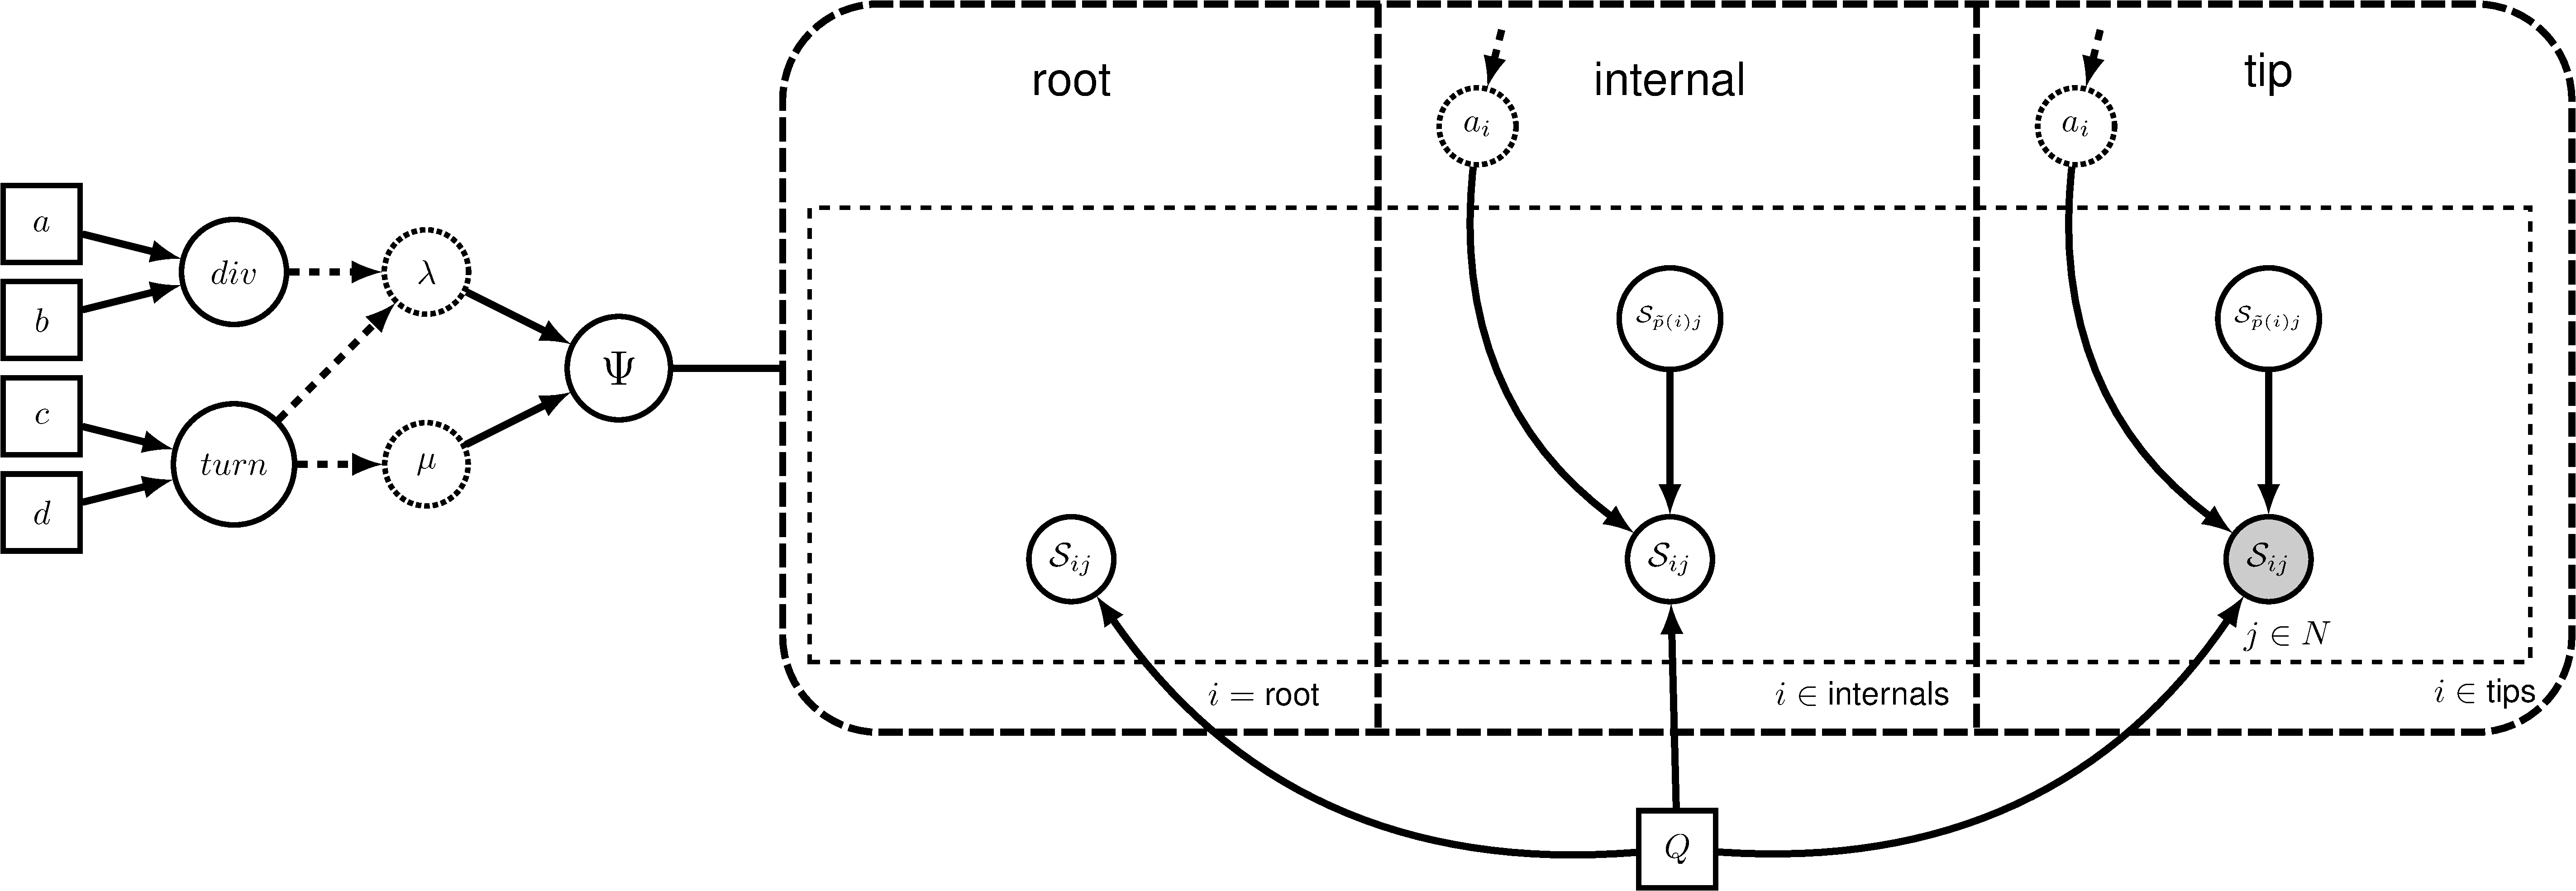
\includegraphics[width=\textwidth,angle=0]{\ResourcePath figures/jc_graphical_model.pdf}}
\caption{\small Graphical model representation of a simple phylogenetic model. 
The graphical model shows the dependencies between the parameters.
Here, the rate matrix $Q$ is a constant variable because it is fixed and does not depend on any parameters.
The only free parameters of this model, the Jukes-Cantor model, are the tree $\Psi$ including the node ages.}
\label{fig:jc}
\end{figure}

We first consider the simplest substitution model described by \cite{Jukes1969}.
The instantaneous-rate matrix for the JC substitution model is defined as
\begin{equation*}
Q_{JC69} = \begin{pmatrix} 
{*} & \frac{1}{3} & \frac{1}{3} & \frac{1}{3} \\ 
\frac{1}{3} & {*} & \frac{1}{3} & \frac{1}{3} \\ 
\frac{1}{3} & \frac{1}{3} & {*} & \frac{1}{3} \\ 
\frac{1}{3} & \frac{1}{3} & \frac{1}{3} & {*}  
\end{pmatrix} \mbox{  ,}
\end{equation*}
which has the advantage that the transition probability matrix can be computed analytically
\begin{equation*}
P_{JC69} = \begin{pmatrix} {{1\over4} + {3\over4}e^{-rt}} & {{1\over4} - {1\over4}e^{-rt}} & {{1\over4} - {1\over4}e^{-rt}} & {{1\over4} - {1\over4}e^{-rt}} \\\\ {{1\over4} - {1\over4}e^{-rt}} & {{1\over4} + {3\over4}e^{-rt}} & {{1\over4} - {1\over4}e^{-rt}} & {{1\over4} - {1\over4}e^{-rt}} \\\\ {{1\over4} - {1\over4}e^{-rt}} & {{1\over4} - {1\over4}e^{-rt}} & {{1\over4} + {3\over4}e^{-rt}} & {{1\over4} - {1\over4}e^{-rt}} \\\\ {{1\over4} - {1\over4}e^{-rt}} & {{1\over4} - {1\over4}e^{-rt}} & {{1\over4} - {1\over4}e^{-rt}} & {{1\over4} + {3\over4}e^{-rt}}  
\end{pmatrix} \mbox{  ,}
\end{equation*}
where $t$ is the branch length in units of time, and $r$ is the rate (clock) for the process.
In the later exercises you will be asked to specify more complex substitution models.
\textbf{Don't be scared by the math!}
\RevBayes will take care of all the computations for you.
Here we only provide some of the equations for the models in case you might be interested in the details.
You will be able to complete the exercises without understanding the underlying math.


\noindent \\ \impmark The files for this example analysis are provided for you, which can easily be run using the \cl{source()} function in the \RevBayes console:
{\tt \begin{snugshade*}
\begin{lstlisting}
source("scripts/mcmc_JC.Rev")
\end{lstlisting}
\end{snugshade*}}

If everything loaded properly, then you should see the program initiate the Markov chain Monte Carlo analysis that estimates the posterior distribution. 
If you continue to let this run, then you will see it output the states of the Markov chain once the MCMC analysis begins. 

Ultimately, this is how you will execute most analyses in \RevBayes, with the full specification of the model and analyses contained in the sourced files. 
You could easily run this entire analysis on your own data by substituting your data file name for that in the model-specification file. 
However, it is important to understand the components of the model to be able to take full advantage of the flexibility and richness of \RevBayes.
Furthermore, without inspecting the \Rev scripts sourced in \cl{mcmc\_JC.Rev}, you may end up inadvertently performing inappropriate analyses on your dataset, which would be a waste of your time and CPU cycles. 
The next steps will walk you through the full specification of the model and MCMC analyses. 

\bigskip

\subsection{Loading the Data}

\noindent \\ \impmark Download data and output files (if you don't have them already) from: \\ \href{http://revbayes.github.io/tutorials.html}{http://revbayes.github.io/tutorials.html}


First load in the sequences using the \cl{readDiscreteCharacterData()} function. 
{\tt \begin{snugshade*}
\begin{lstlisting}
data <- readDiscreteCharacterData("data/primates_and_galeopterus_cytb.nex")
\end{lstlisting}
\end{snugshade*}}
Executing these lines initializes the data matrix as the respective \Rev variables. 
To report the current value of any variable, simply type the variable name and press enter. For the \cl{data} matrix, this provides information about the alignment:
{\tt \begin{snugshade*}
\begin{lstlisting}
data
|*   DNA character matrix with 23 taxa and 1141 characters
|*   =====================================================
|*   Origination:                      primates_and_galeopterus_cytb.nex
|*   Number of taxa:                   23
|*   Number of included taxa:          23
|*   Number of characters:             1141
|*   Number of included characters: 1141
|*   Datatype:                         DNA
\end{lstlisting}
\end{snugshade*}}


Next we will specify some useful variables based on our dataset. The variable \cl{data} has \emph{member functions} that we can use to retrieve information about the dataset. 
These include, for example, the number of species and the taxa.
We will need that taxon information for setting up different parts of our model.
{\tt \begin{snugshade*}
\begin{lstlisting}
n_species <- data.ntaxa()
n_branches <- 2 * n_species - 3
taxa <- data.taxa()
\end{lstlisting}
\end{snugshade*}}

Additionally, we set up a counter variable for the number of moves that we already added to our analysis.
[Recall that moves are algorithms used to propose new parameter values during the MCMC simulation.]
This will make it much easier if we extend the model or analysis to include additional moves or to remove some moves.
Similarly, we set up a counter variable for the number of monitors. 
[Monitors print the values of model parameters to the screen and/or log files during the MCMC analysis].
{\tt \begin{snugshade*}
\begin{lstlisting}
mvi = 0 
mni = 0
\end{lstlisting}
\end{snugshade*}}
You may have noticed that we used the \cl{=} operator to create the move index.
This simply means that the variable is not part of the model.
You will later see that we use this operator more often, \EG when we create moves and monitors.

With the data loaded, we can now proceed to specify our Jukes-Cantor substitution model.

\subsection{Jukes-Cantor Substitution Model}

A given substitution model is defined by its corresponding instantaneous-rate matrix, $Q$.
The Jukes-Cantor substitution model does not have any free parameters (as the substitution rates are all assumed to be equal), so we can define it as a constant variable.
The function \cl{fnJC(n)} will create an instantaneous-rate matrix for character with $n$ states.
Since we use DNA data here, we create a 4x4 instantaneous-rate matrix:
{\tt \begin{snugshade*}
\begin{lstlisting}
Q <- fnJC(4) 
\end{lstlisting}
\end{snugshade*}}
You can see the rates of the $Q$ matrix by typing
{\tt \begin{snugshade*}
\begin{lstlisting}
Q
|*   [ [ -1.0000, 0.3333, 0.3333, 0.3333 ] ,
|*     0.3333, -1.0000, 0.3333, 0.3333 ] ,
|*     0.3333, 0.3333, -1.0000, 0.3333 ] ,
|*     0.3333, 0.3333, 0.3333, -1.0000 ] ]
\end{lstlisting}
\end{snugshade*}}
As you can see, all substitution rates are equal.


\bigskip
\subsection{Tree Topology and Branch Lengths}

The tree topology and branch lengths are stochastic nodes in our phylogenetic model. 
In Figure \ref{fig:jc}, the tree topology is denoted $\Psi$ and the length of the branch leading to node $i$ is $bl_i$.

We will assume that all possible labeled, unrooted tree topologies have equal probability. 
This is the \cl{dnUniformTopology()} distribution in \RevBayes. 
Note that in \RevBayes it is advisable to specify the outgroup for your study system if you use an unrooted tree prior, whereas other software, \EG \MrBayes uses the first taxon in the data matrix file as the outgroup.
Specify the \cl{topology} stochastic node by passing in the tip labels \cl{names} to the \cl{dnUniformTopology()} distribution:
{\tt \begin{snugshade*}
\begin{lstlisting}
out_group = clade("Galeopterus_variegatus")
topology ~ dnUniformTopology(taxa, outgroup=out_group)
\end{lstlisting}
\end{snugshade*}}

Some types of stochastic nodes can be updated by a number of alternative moves. 
Different moves may explore parameter space in different ways, and it is possible to use multiple different moves for a given parameter to improve mixing (the efficiency of the MCMC simulation). 
In the case of our unrooted tree topology, for example, we can use both a nearest-neighbor interchange move (\cl{mvNNI}) and a subtree-prune and regrafting move (\cl{mvSPR}). 
These moves do not have tuning parameters associated with them, thus you only need to pass in the \cl{topology} node and proposal \cl{weight}. 
{\tt \begin{snugshade*}
\begin{lstlisting}
moves[++mvi] = mvNNI(topology, weight=1.0)
moves[++mvi] = mvSPR(topology, weight=1.0)
\end{lstlisting}
\end{snugshade*}}
The weight specifies how often the move will be applied either on average per iteration or relative to all other moves.
Have a look at the \href{https://github.com/revbayes/revbayes_tutorial/raw/master/tutorial_TeX/RB_MCMC_Tutorial/RB_MCMC_Tutorial.pdf}{MCMC Diagnosis tutorial} for more details about moves and MCMC strategies (found on the \href{http://revbayes.github.io/tutorials.html}{\RevBayes~Tutorials Website}).


Next we have to create a stochastic node for each of the $2N-3$ branches in our tree (where $N=$ \cl{n\_species}). 
We can do this using a \cl{for} loop --- this is a plate in our graphical model. In this loop, we can create each of the branch-length nodes and assign each move. 
Copy this entire block of \Rev~code into the console:
{\tt \small \begin{snugshade*}
\begin{lstlisting}
for (i in 1:n_branches) {
   br_lens[i] ~ dnExponential(10.0)
   moves[++mvi] = mvScale(br_lens[i]) 
}
\end{lstlisting}
\end{snugshade*}}

It is convenient for monitoring purposes to add the tree length as deterministic variable. 
The tree length is simply the sum of all branch lengths. 
%This parameter is denoted $\mathbb{L}$ in Figure \ref{fig:jc}.
Accordingly, the tree length can be computed using the \cl{sum()} function, which calculates the sum of any vector of values.
{\tt \begin{snugshade*}
\begin{lstlisting}
TL := sum(br_lens)
\end{lstlisting}
\end{snugshade*}}

\begin{framed}
\textbf{Alternative branch-length priors}\\
Some studies, \EG \cite{Brown2010,Rannala2012}, have criticized the exponential prior distribution for branch lengths because it induces a gamma-dsitributed tree-length and the mean of this gamma distribution grows with the number of taxa.
For example, we can use instead a specific gamma prior distribution (or any other distribution defined on a positive real variable) for the tree length, and then use a Dirichlet prior distribution to break the tree length into the corresponding branch lengths \citep{Zhang2012}.
{\tt \begin{snugshade*}
\begin{lstlisting}
# specify a prior distribution on the tree length with your desired mean
TL ~ dnGamma(2,4)
moves[++mvi] = mvScale(TL) 

# now create a random variable for the relative branch lengths
rel_branch_lengths ~ dnDirichlet( rep(1.0,n_branches) )
moves[++mvi] = mvBetaSimplex(rel_branch_lengths, weight=n_branches)
moves[++mvi] = mvDirichletSimplex(rel_branch_lengths, weight=n_branches/10.0)

# finally, transform the relative branch lengths into actual branch lengths
br_lens := rel_branch_lengths * TL
\end{lstlisting}
\end{snugshade*}}
\end{framed}


Finally, we can create a \emph{phylogram} (a phylogeny in which the branch lengths are proportional to the expected number of substitutions/site) by combining the tree topology and branch lengths.
We do this using the \cl{treeAssembly()} function, which applies the value of the $i^{th}$ member of the \cl{br\_lens} vector to the branch leading to the $i^{th}$ node in \cl{topology}. 
Thus, the \cl{psi} variable is a deterministic node: 

{\tt \begin{snugshade*}
\begin{lstlisting}
psi := treeAssembly(topology, br_lens)
\end{lstlisting}
\end{snugshade*}}

\begin{framed}
\textbf{Prior on Time-Trees: Tree Topology and Node Ages}\\
Alternatively, you may want to specify a prior on time-trees.
Here we will briefly indicate how to specify such an prior which will lead to inference of time trees.

The tree (the topology and node ages) is a stochastic node in our phylogenetic model. 
For simplicity, we will assume a uniform prior on both topologies and node ages.
The distribution in \RevBayes is \cl{dnUniformTimeTree()}. 

\impmark{Fore more information on tree priors, such as birth-death processes, please read the \href{https://github.com/revbayes/revbayes_tutorial/raw/master/tutorial_TeX/RB_DiversificationRate_Tutorial/RB_DiversificationRate_Tutorial.pdf}{RB\_DiversificationRate\_Tutorial}.}

First, we need to specify the age of the tree:
{\tt \begin{snugshade*}
\begin{lstlisting}
root_age <- 10.0
\end{lstlisting}
\end{snugshade*}}
Here we simply assumed that the tree is 10.0 time units old. 
We could also specify a prior on the root age if we have fossil calibrations (see \href{https://github.com/revbayes/revbayes_tutorial/raw/master/tutorial_TeX/RB_DivergenceTime_Calibration_Tutorial/RB_DivergenceTime_Calibration_Tutorial.pdf}{Divergence Time and Calibration Tutorial})
Next, we specify the \cl{tree} stochastic variable by passing in the taxon information \cl{taxa} to the \cl{dnUniformTimeTree()} distribution:
{\tt \begin{snugshade*}
\begin{lstlisting}
psi ~ dnUniformTimeTree(rootAge=root_age, taxa=taxa)
\end{lstlisting}
\end{snugshade*}}

Some types of stochastic nodes can be updated by a number of alternative moves. 
Different moves may explore parameter space in different ways, and it is possible to use multiple different moves for a given parameter to improve mixing (the efficiency of the MCMC simulation). 
In the case of our rooted tree, for example, we can use both a nearest-neighbor interchange move without and with changing the node ages (\cl{mvNarrow} and \cl{mvNNI}) and a fixed-nodeheight subtree-prune and regrafting move (\cl{mvFNPR}) and its Metropolized-Gibbs variant (\cl{mvGPR}) \citep{Hoehna2008,Hoehna2012}. 
We also need moves that change the ages of the internal nodes; which are for example the \cl{mvSubtreeScale} and \cl{mvNodeTimeSlideUniform}.
These moves do not have tuning parameters associated with them, thus you only need to pass in the \cl{psi} node and proposal \cl{weight}. 
{\tt \begin{snugshade*}
\begin{lstlisting}
moves[++mvi] = mvNarrow(psi, weight=5.0)
moves[++mvi] = mvNNI(psi, weight=1.0)
moves[++mvi] = mvFNPR(psi, weight=3.0)
moves[++mvi] = mvGPR(psi, weight=3.0)
moves[++mvi] = mvSubtreeScale(psi, weight=3.0)
moves[++mvi] = mvNodeTimeSlideUniform(psi, weight=15.0)
\end{lstlisting}
\end{snugshade*}}
The weight specifies how often the move will be applied either on average per iteration or relative to all other moves.
Have a look at the MCMC tutorial for more details about moves and MCMC strategies: \href{http://revbayes.github.io/tutorials.html}{http://revbayes.github.io/tutorials.html}
\vspace{0.3cm}

\textbf{Molecular clock}\\
Additionally, in the case of time-calibrated trees, we need to add a molecular clock rate parameter.
For example, we know from empirical estimates that the molecular clock rate is about  0.01 (=1\%) per million years per site.
Nevertheless, we can estimate it here because we fixed the root age.
We use a uniform prior on the log-transform clock rate.
This specifies our lack of prior knowledge on the magnitude of the clock rate.
{\tt \begin{snugshade*}
\begin{lstlisting}
log_clock_rate ~ dnUniform(-6,1)
moves[++mvi] = mvSlide(log_clock_rate, weight=2.0)
clock_rate := 10^log_clock_rate
\end{lstlisting}
\end{snugshade*}}

Instead, you could also fix the clock rate and estimate the root age.
\impmark{Fore more information on molecular clocks please read the \href{https://github.com/revbayes/revbayes_tutorial/raw/master/tutorial_TeX/RB_DivergenceTime_Tutorial/RB_DivergenceTime_Tutorial.pdf}{RB\_DivergenceTime\_Tutorial}.}

\end{framed}


\subsection{Putting it All Together}

We have fully specified all of the parameters of our phylogenetic model---the tree topology with branch lengths, and the substitution model that describes how the sequence data evolved over the tree with branch lengths.  
Collectively, these parameters comprise a distribution called the \textit{phylogenetic continuous-time Markov chain}, and we use the \cl{dnPhyloCTMC} constructor function to create this node.
This distribution requires several input arguments: 
(1) the \cl{tree} with branch lengths; 
(2) the instantaneous-rate matrix \cl{Q};
(3) the \cl{type} of character data.


Build the random variable for the character data (sequence alignment).
{\tt \begin{snugshade*}
\begin{lstlisting}
# the sequence evolution model
seq ~ dnPhyloCTMC(tree=psi, Q=Q, type="DNA")
\end{lstlisting}
\end{snugshade*}}


Once the \cl{PhyloCTMC} model has been created, we can attach our sequence data to the tip nodes in the tree.
{\tt \begin{snugshade*}
\begin{lstlisting}
seq.clamp(data)
\end{lstlisting}
\end{snugshade*}}
[Note that although we assume that our sequence data are random variables---they are realizations of our phylogenetic model---for the purposes of inference, we assume that the sequence data are ``clamped''.]
When this function is called, \RevBayes sets each of the stochastic nodes representing the tips of the tree to the corresponding nucleotide sequence in the alignment. 
This essentially tells the program that we have observed data for the sequences at the tips. 

Finally, we wrap the entire model to provide convenient access to the DAG. 
To do this, we only need to give the \cl{model()} function a single node. 
With this node, the \cl{model()} function can find all of the other nodes by following the arrows in the graphical model:
{\tt \begin{snugshade*}
\begin{lstlisting}
mymodel = model(Q)
\end{lstlisting}
\end{snugshade*}}

Now we have specified a simple phylogenetic analysis---each parameter of the model will be estimated from every site in our alignment.
If we inspect the contents of \cl{mymodel} we can review all of the nodes in the DAG:
{\tt \begin{snugshade*}
\begin{lstlisting}
mymodel
\end{lstlisting}
\end{snugshade*}}

\bigskip
\subsection{Performing an MCMC Analysis Under the Jukes-Cantor Model}

In this section, will describe how to set up the MCMC sampler and summarize the resulting posterior distribution of trees. 

\subsubsection{Specifying Monitors}

For our MCMC analysis, we need to set up a vector of \textit{monitors} to record the states of our Markov chain. 
The monitor functions are all called \cl{mn*}, where \cl{*} is the wildcard representing the monitor type.
First, we will initialize the model monitor using the \cl{mnModel} function. This creates a new monitor variable that will output the states for all model parameters when passed into a MCMC function. 
{\tt \begin{snugshade*}
\begin{lstlisting}
monitors[++mni] = mnModel(filename="output/primates_cytb_JC_posterior.log",printgen=10, separator = TAB)
\end{lstlisting}
\end{snugshade*}}

The \cl{mnFile} monitor will record the states for only the parameters passed in as arguments. We use this monitor to specify the output for our sampled trees and branch lengths.

{\tt \begin{snugshade*}
\begin{lstlisting}
monitors[++mni] = mnFile(filename="output/primates_cytb_JC_posterior.trees",printgen=10, separator = TAB, psi)
\end{lstlisting}
\end{snugshade*}}


Finally, create a screen monitor that will report the states of specified variables to the screen with \cl{mnScreen}:
{\tt \begin{snugshade*}
\begin{lstlisting}
monitors[++mni] = mnScreen(printgen=1000, TL)
\end{lstlisting}
\end{snugshade*}}
This monitor mostly helps us to see the progress of the MCMC run.

\subsubsection{Initializing and Running the MCMC Simulation}

With a fully specified model, a set of monitors, and a set of moves, we can now set up the MCMC algorithm that will sample parameter values in proportion to their posterior probability. 
The \cl{mcmc()} function will create our MCMC object:
{\tt \begin{snugshade*}
\begin{lstlisting}
mymcmc = mcmc(mymodel, monitors, moves, nruns=2)
\end{lstlisting}
\end{snugshade*}}
Notice that we also specified \cl{nruns=2} which means that \RevBayes will automatically run 2 independent MCMC runs.
You will find that the output is created in two files with extension \cl{\_run\_1} and \cl{\_run\_2} for each replicate and additionally the samples from both runs are combined into one file for more convenient post-processing.

We may wish to run the \cl{.burnin()} member function.
Recall that this function \textbf{does not} specify the number of states that we wish to discard from the MCMC analysis as burnin (i.e., the samples collected before the chain converges to the stationary distribution).  
Instead, the \cl{.burnin()} function specifies a \textit{completely separate} preliminary MCMC analysis that is used to tune the scale of the moves to improve mixing of the MCMC analysis.
{\tt \begin{snugshade*}
\begin{lstlisting}
mymcmc.burnin(generations=10000,tuningInterval=1000)
\end{lstlisting}
\end{snugshade*}}


Now, run the MCMC:
{\tt \begin{snugshade*}
\begin{lstlisting}
mymcmc.run(generations=30000)
\end{lstlisting}
\end{snugshade*}}

When the analysis is complete, you will have the monitored files in your output directory.


Methods for visualizing the marginal densities of parameter values are not currently available in \RevBayes itself. 
Thus, it is important to use programs like \Tracer \citep{Rambaut2011} to evaluate mixing and non-convergence.

\noindent \\ \impmark Look at the files called \cl{output/primates\_cytb\_JC\_posterior\_run\_1.log} and \\\cl{output/primates\_cytb\_JC\_posterior\_run\_2.log} in \Tracer. There you see the posterior distributions of the continuous parameters, \EG the tree length variable \cl{TL}.
\begin{figure}[htbp!]
\centering
\fbox{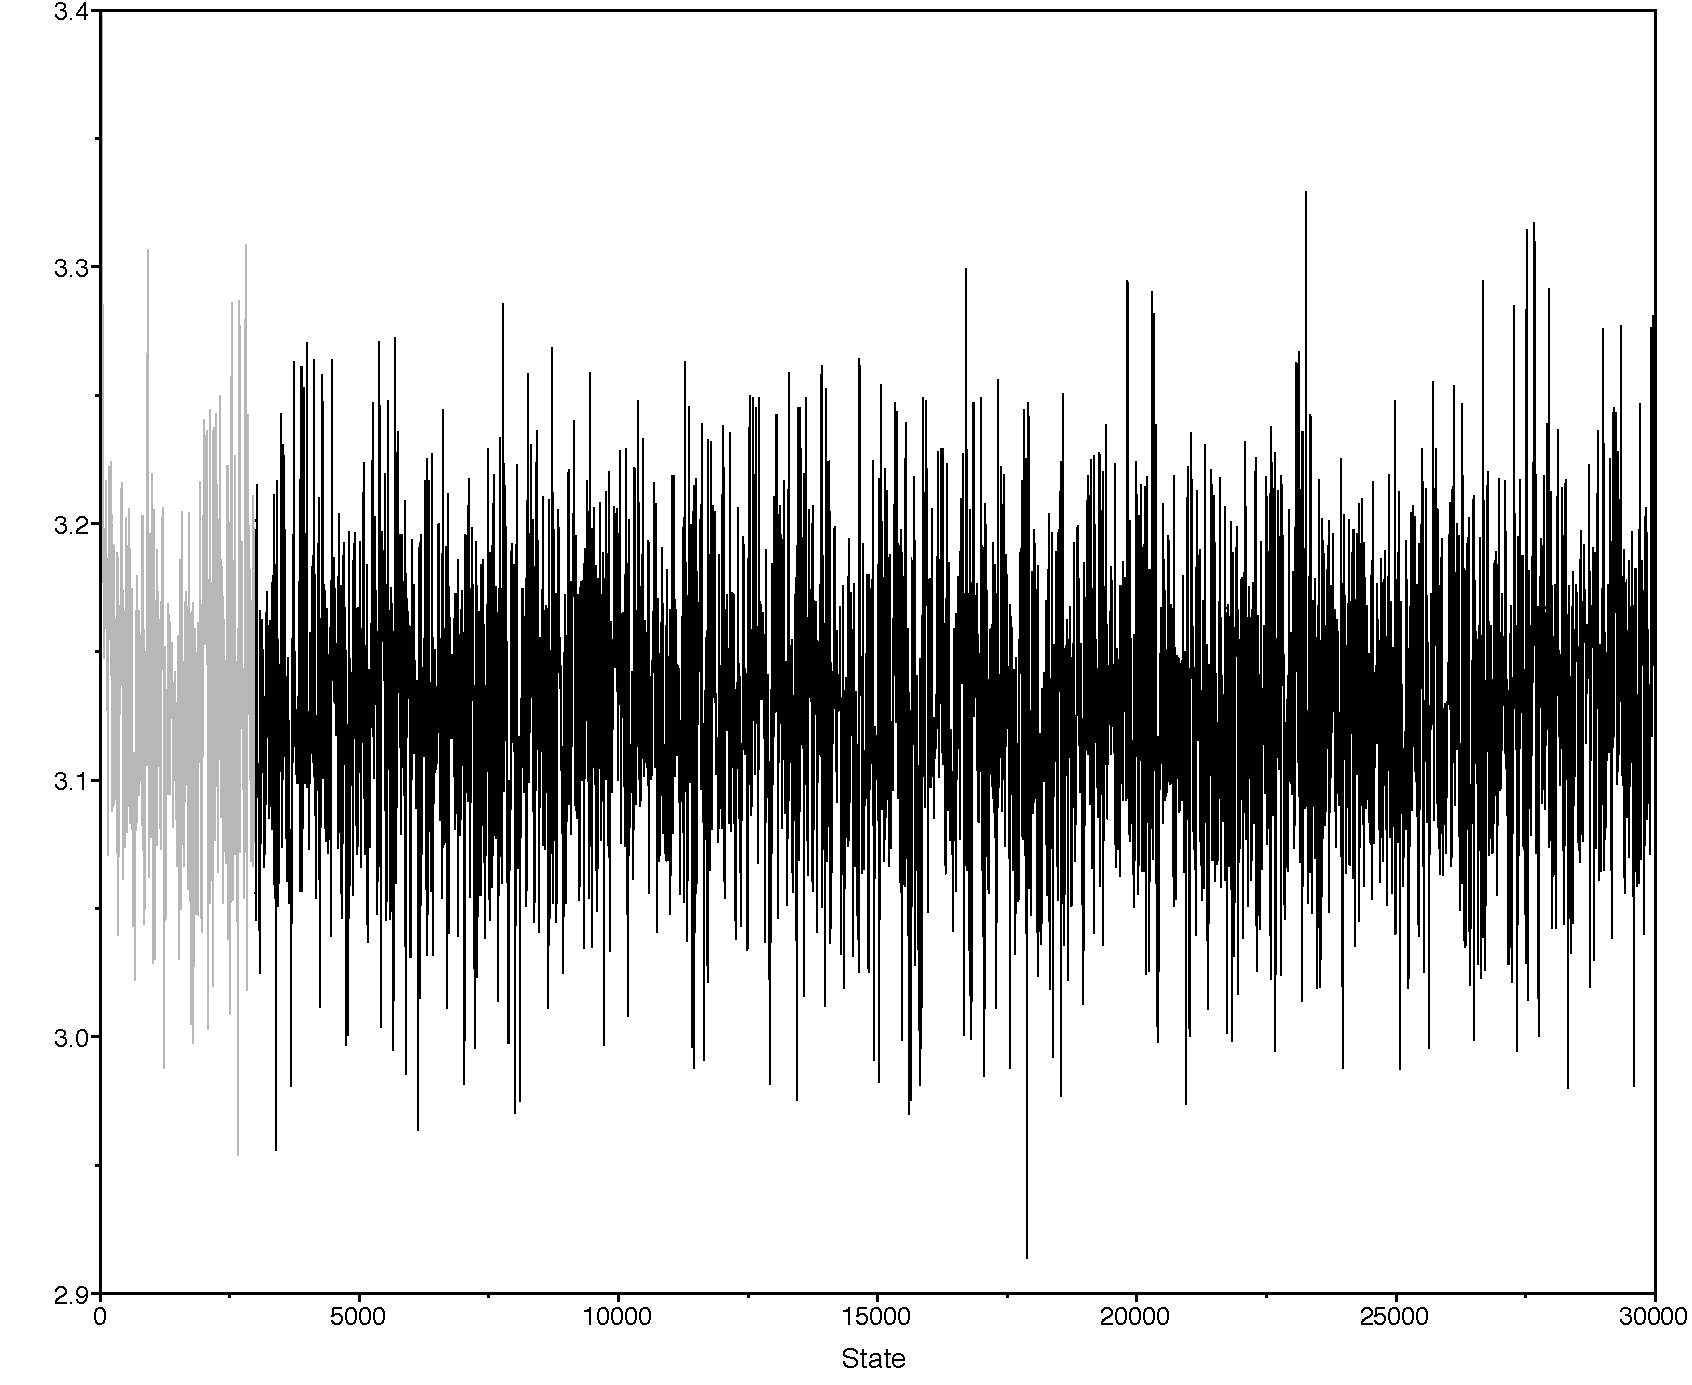
\includegraphics[width=0.4\textwidth]{\ResourcePath figures/primates_cytb_JC_TL_Trace.pdf}
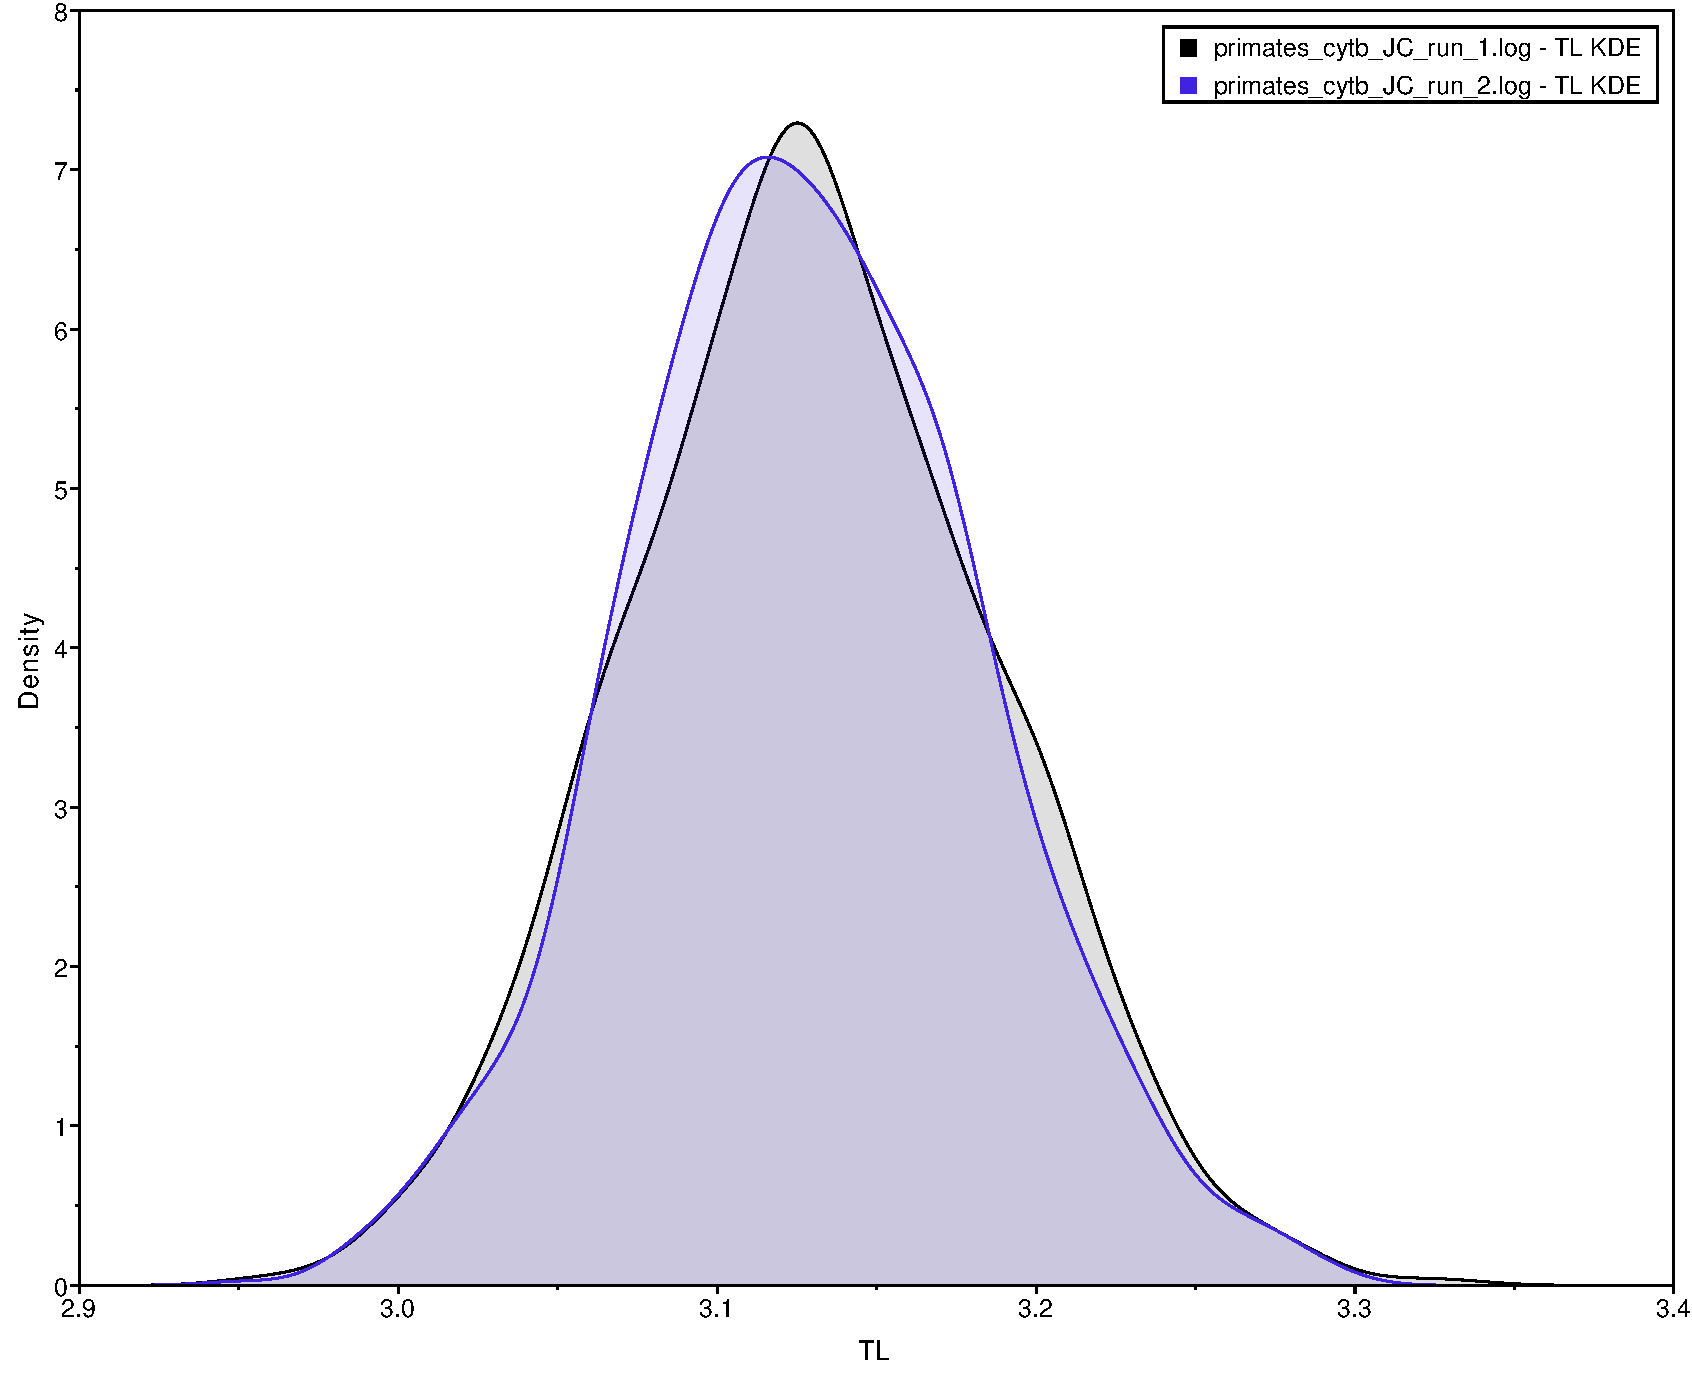
\includegraphics[width=0.4\textwidth]{\ResourcePath figures/primates_cytb_JC_TL_Distribution.pdf}}
\caption{\small Left: Trace of tree-length samples for the two replicated MCMC runs. 
The caterpillar-like look is a good sign as well as as that the two runs look virtually identical.
You will also see that the effective sample size is comparably large, \IE much larger than 200.
Right: Posterior distribution of the tree length of the primate phylogeny under a Jukes-Cantor substitution model. 
Here we show the two independent replicated MCMC runs which yield the same posterior estimate.
This is a superficial test that the MCMC has converged to the same estimate.}
\label{fig:jc_tree}
\end{figure}

\subsection{Exercise 1}

We are interested in the phylogenetic relationship of the Tarsiers. Therefore, we need to summarize the trees sampled from the posterior distribution.
\RevBayes can summarize the sampled trees by reading in the tree-trace file:
{\tt \begin{snugshade*}
\begin{lstlisting}
treetrace = readTreeTrace("output/primates_cytb_JC_posterior.trees",
                             treetype="non-clock")
treetrace.summarize()
\end{lstlisting}
\end{snugshade*}}
The \cl{mapTree()} function will summarize the tree samples and write the maximum \textit{a posteriori} tree to file:
{\tt \begin{snugshade*}
\begin{lstlisting}
map_tree = mapTree(treetrace,"output/primates_cytb_JC_MAP.tree")
\end{lstlisting}
\end{snugshade*}}
\begin{figure}[htbp!]
\centering
\fbox{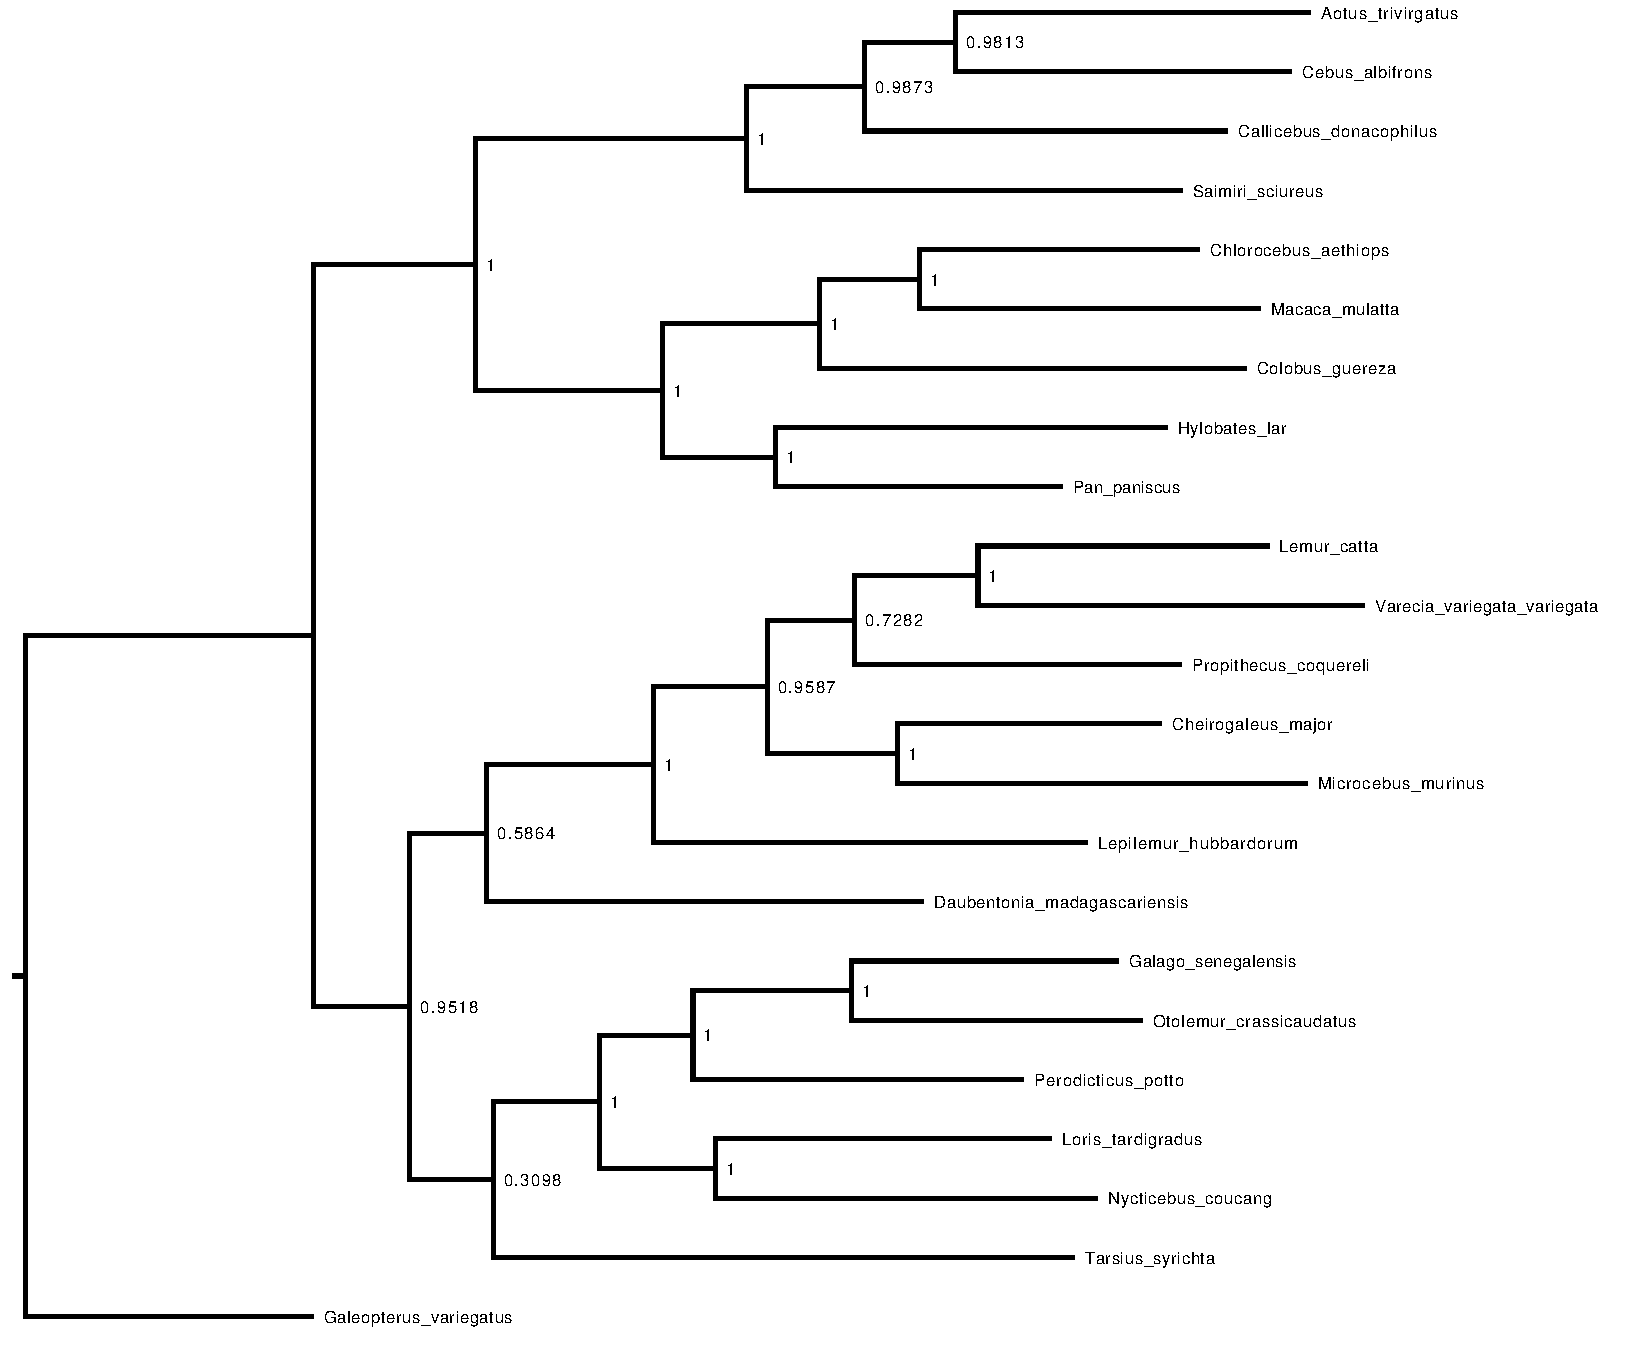
\includegraphics[width=0.8\textwidth]{\ResourcePath figures/primates_cytb_JC_tree.pdf}}
\caption{\small Maximum a posteriori estimate of the primate phylogeny under a Jukes-Cantor substitution model. 
The numbers at the nodes show the posterior probabilities for the clades.
We have rooted the tree at the outgroup \emph{Galeopterus\_variegatus}}
\label{fig:jc_tree}
\end{figure}
\noindent \\ \impmark Look at the file called \cl{output/primates\_cytb\_JC.tree} in \texttt{FigTree}. We show it in Figure~\ref{fig:jc_tree}.


\noindent \\ \impmark Fill in the following table as you go through the tutorial.

\begin{Form}
\begin{table}[h!]
\centering
\caption{\small Posterior probabilities of phylogenetic relationship$^*$.}
\resizebox{\textwidth}{!}{%
\begin{tabular}{l c c c c}
\hline
\textbf{Model} & \textit{Lemuroidea} & \textit{Lorisoidea} & \textit{Platyrrhini} & \textit{Catarrhini} \\ 
\hline
\vspace{1mm}
Jukes-Cantor & \TextField[name=pp11,backgroundcolor={.85 .85 .85},color={1 0 0},height=4ex]{}  & \TextField[name=pp12,backgroundcolor={.85 .85 .85},color={0 0 1},height=4ex]{}  & \TextField[name=pp13,backgroundcolor={.85 .85 .85},color={0 0 1},height=4ex]{}  & \TextField[name=pp14,backgroundcolor={.85 .85 .85},color={0 0 1},height=4ex]{}\\
\hline
\vspace{1mm}
HKY85 & \TextField[name=pp21,backgroundcolor={.85 .85 .85},color={1 0 0},height=4ex]{}  & \TextField[name=pp22,backgroundcolor={.85 .85 .85},color={0 0 1},height=4ex]{}  & \TextField[name=pp23,backgroundcolor={.85 .85 .85},color={0 0 1},height=4ex]{}  & \TextField[name=pp24,backgroundcolor={.85 .85 .85},color={0 0 1},height=4ex]{} \\
\hline
\vspace{1mm}
F81 & \TextField[name=pp31,backgroundcolor={.85 .85 .85},color={1 0 0},height=4ex]{}  & \TextField[name=pp32,backgroundcolor={.85 .85 .85},color={0 0 1},height=4ex]{}  & \TextField[name=pp33,backgroundcolor={.85 .85 .85},color={0 0 1},height=4ex]{}  & \TextField[name=pp34,backgroundcolor={.85 .85 .85},color={0 0 1},height=4ex]{} \\
\hline
\vspace{1mm}
GTR & \TextField[name=pp41,backgroundcolor={.85 .85 .85},color={1 0 0},height=4ex]{}  & \TextField[name=pp42,backgroundcolor={.85 .85 .85},color={0 0 1},height=4ex]{}  & \TextField[name=pp43,backgroundcolor={.85 .85 .85},color={0 0 1},height=4ex]{}  & \TextField[name=pp44,backgroundcolor={.85 .85 .85},color={0 0 1},height=4ex]{} \\
\hline
\vspace{1mm}
GTR+$\Gamma$ & \TextField[name=pp51,backgroundcolor={.85 .85 .85},color={1 0 0},height=4ex]{}  & \TextField[name=pp52,backgroundcolor={.85 .85 .85},color={0 0 1},height=4ex]{}  & \TextField[name=pp53,backgroundcolor={.85 .85 .85},color={0 0 1},height=4ex]{}  & \TextField[name=pp54,backgroundcolor={.85 .85 .85},color={0 0 1},height=4ex]{} \\
\hline
\vspace{1mm}
GTR+$\Gamma$+I & \TextField[name=pp61,backgroundcolor={.85 .85 .85},color={1 0 0},height=4ex]{}  & \TextField[name=pp62,backgroundcolor={.85 .85 .85},color={0 0 1},height=4ex]{}  & \TextField[name=pp63,backgroundcolor={.85 .85 .85},color={0 0 1},height=4ex]{}  & \TextField[name=pp64,backgroundcolor={.85 .85 .85},color={0 0 1},height=4ex]{} \\
\hline
{\footnotesize{$^*$you can edit this table}}\\
\end{tabular}}
\label{tab:pp}
\end{table}
\end{Form}

\begin{table}[h!]
\centering
\caption{\small Primate species and famaly relationships.}
\begin{tabular}{l l l l}
\hline
\textbf{Species} & \textbf{Family} & \textbf{Parvorder} & \textbf{Suborder} \\ 
\hline
%Alouatta palliata & Atelidae & Platyrrhini (NWM) & Haplorrhini \\
Aotus trivirgatus & Aotidae & Platyrrhini (NWM) & Haplorrhini \\
Callicebus donacophilus & Pitheciidae & Platyrrhini (NWM) & Haplorrhini \\
Cebus albifrons & Cebidae & Platyrrhini (NWM) & Haplorrhini \\
Cheirogaleus major & Cheirogaleidae & Lemuroidea & Strepsirrhini \\
Chlorocebus aethiops & Cercopithecoidea & Catarrhini & Haplorrhini \\
Colobus guereza & Cercopithecoidea & Catarrhini & Haplorrhini \\
Daubentonia madagascariensis & Daubentoniidae & Lemuroidea & Strepsirrhini \\
Galago senegalensis & Galagidae & Lorisidae & Strepsirrhini \\
Hylobates lar & Hylobatidea & Catarrhini & Haplorrhini \\
Lemur catta & Lemuridae & Lemuroidea & Strepsirrhini \\
Lepilemur hubbardorum & Lepilemuridae & Lemuroidea & Strepsirrhini \\
Loris tardigradus & Lorisidae & Lorisidae & Strepsirrhini \\
Macaca mulatta & Cercopithecoidea & Catarrhini & Haplorrhini \\
Microcebus murinus & Cheirogaleidae & Lemuroidea & Strepsirrhini \\
Nycticebus coucang & Lorisidae & Lorisidae & Strepsirrhini \\
Otolemur crassicaudatus & Galagidae & Lorisidae & Strepsirrhini \\
Pan paniscus & Hominoidea & Catarrhini & Haplorrhini \\
Perodicticus potto & Lorisidae & Lorisidae & Strepsirrhini \\
Propithecus coquereli & Indriidae & Lemuroidea & Strepsirrhini \\
Saimiri sciureus & Cebidae & Platyrrhini (NWM) & Haplorrhini \\
Tarsius syrichta & Tarsiidae &  & Haplorrhini \\
Varecia variegata variegata & Lemuridae & Lemuroidea & Strepsirrhini \\
\hline
\end{tabular}
\label{tab:primates}
\end{table}




\newpage
\section{The Hasegawa-Kishino-Yano (HKY) 1985 Substitution Model}

The Jukes-Cantor model assumes that all substitution rates are equal, which also implies that the stationary frequencies of the four nucleotide bases are equal.
These assumptions are not very biologically reasonable, so we might wish to consider a more realistic substitution model that relaxes some of these assumptions.
For example, we might allow stationary frequencies, $\pi$, to be unequal, and allow rates of transition and transversion substitutions to differ, $\kappa$.
This corresponds to the substitution model proposed by \citet[][HKY]{Hasegawa1985}, which is specified with the following instantaneous-rate matrix: 
\begin{equation*}
Q_{HKY} = \begin{pmatrix} 
{\cdot} 			& {\pi_C} 	& {\kappa\pi_G} 			& {\pi_T} \\ 
{\pi_A} 		& {\cdot} 			& {\pi_C} 			& {\kappa\pi_T} \\ 
{\kappa\pi_A} 			& {\pi_C} 			& {\cdot} 			& {\pi_T} \\ 
{\pi_A} 			& {\kappa\pi_C} 			& {\pi_G} 	& {\cdot}  
\end{pmatrix} \mbox{  .}
\end{equation*}
[The diagonal ${\cdot}$ entries are equal to the negative sum of the elements in the corresponding row.] 

\noindent \\ \impmark Use the file \cl{mcmc\_JC.Rev} as a starting point for the HKY analysis.

Note that we are adding two new variables to our model.
We can define a variable \cl{pi} for the stationary frequencies that are drawn from a flat Dirichlet distribution by
{\tt \begin{snugshade*}
\begin{lstlisting}
pi_prior <- v(1,1,1,1) 
pi ~ dnDirichlet(pi_prior)
\end{lstlisting}
\end{snugshade*}}
Since \cl{pi} is a stochastic variable, we need to specify a move to propose updates to it.
A good move on variables drawn from a Dirichlet distribution is the \cl{mvBetaSimplex}.
This move randomly takes an element from the simplex, proposes a new value for it drawn from a Beta distribution, and then rescales all values of the simplex to sum to 1 again.
{\tt \begin{snugshade*}
\begin{lstlisting}
moves[++mvi] = mvBetaSimplex(pi, weight=2)
moves[++mvi] = mvDirichletSimplex(pi, weight=1)
\end{lstlisting}
\end{snugshade*}}

The second new variable is $\kappa$, which specifies the ratio of transition-transversion rates.
The $\kappa$ parameter must be a positive-real number and a natural choice as the prior distribution is the lognormal distribution:
{\tt \begin{snugshade*}
\begin{lstlisting}
kappa ~ dnLognormal(0.0,1.25)
\end{lstlisting}
\end{snugshade*}}
Again, we need to specify a move for this new stochastic variable.
A simple scaling move should do the job.
{\tt \begin{snugshade*}
\begin{lstlisting}
moves[++mvi] = mvScale(kappa)
\end{lstlisting}
\end{snugshade*}}

Finally, we need to create the HKY instantaneous-rate matrix using the \cl{fnHKY} function:
{\tt \begin{snugshade*}
\begin{lstlisting}
Q := fnHKY(kappa,pi)
\end{lstlisting}
\end{snugshade*}}
This should be all for the HKY model.

\noindent \\ \impmark Don't forget to change the output file names, otherwise your old analyses files will be overwritten.

\subsection{Exercise 2}

\begin{itemize}
\item Copy the file called  \cl{mcmc\_JC.Rev} and modify it by including the necessary parameters to specify the HKY substitution model.
\item Run an MCMC analysis to estimate the posterior distribution under the HKY substitution model.
\item Are the resulting estimates of the base frequencies equal? 
	If not, how much do they differ? 
	Are the estimated base frequencies similar to the empirical base frequencies? 
	The empirical base frequencies are the frequencies of the characters in the alignment, which can be computed with \RevBayes by \cl{data.getEmpiricalBaseFrequencies()}.
\item Is the inferred rate of transition substitutions higher than the rate of transversion substitutions? If so, by how much?
\item Like the HKY model, the Felsenstein 1981 (F81) substitution model has unequal stationary frequencies, but it assumes equal transition-transversion rates \citep{Felsenstein1981}.
	Can you set up the F81 model and run an analysis?
\item Complete the table of the phylogenetic relationship of primates.
\end{itemize}






\newpage
\section{The General Time-Reversible (GTR) Substitution Model}

The HKY substitution model can accommodate unequal base frequencies and different rates of transition and transversion substitutions.
Despite these extensions, the HKY model may still be too simplistic for many real datasets.
Here, we extend the HKY model to specify the General Time Reversible (GTR) substitution model \citep{Tavare1986}, which allows all six exchangeability rates to differ (Figure \ref{fig:gtr}).

The instantaneous-rate matrix for the GTR substitution model is:
\begin{equation*}
\resizebox{4in}{!}{%  
$Q_{GTR} = \begin{pmatrix}
{\cdot}	   & {r_{AC}\pi_C} & {r_{AG}\pi_G} & {r_{AT}\pi_T} \\
{r_{AC}\pi_A} & {\cdot}       & {r_{CG}\pi_G} & {r_{CT}\pi_T} \\
{r_{AC}\pi_A} & {r_{CG}\pi_C} & {\cdot}       & {r_{GT}\pi_T} \\
{r_{AC}\pi_A} & {r_{CT}\pi_C} & {r_{GT}\pi_G} & {\cdot}       \\
\end{pmatrix} \mbox{  ,} $}
\end{equation*}

where the six exchangeability parameters, $r_{ij}$, specify the relative rates of change between states $i$ and $j$.  


\begin{figure}[h!]
\centering
\fbox{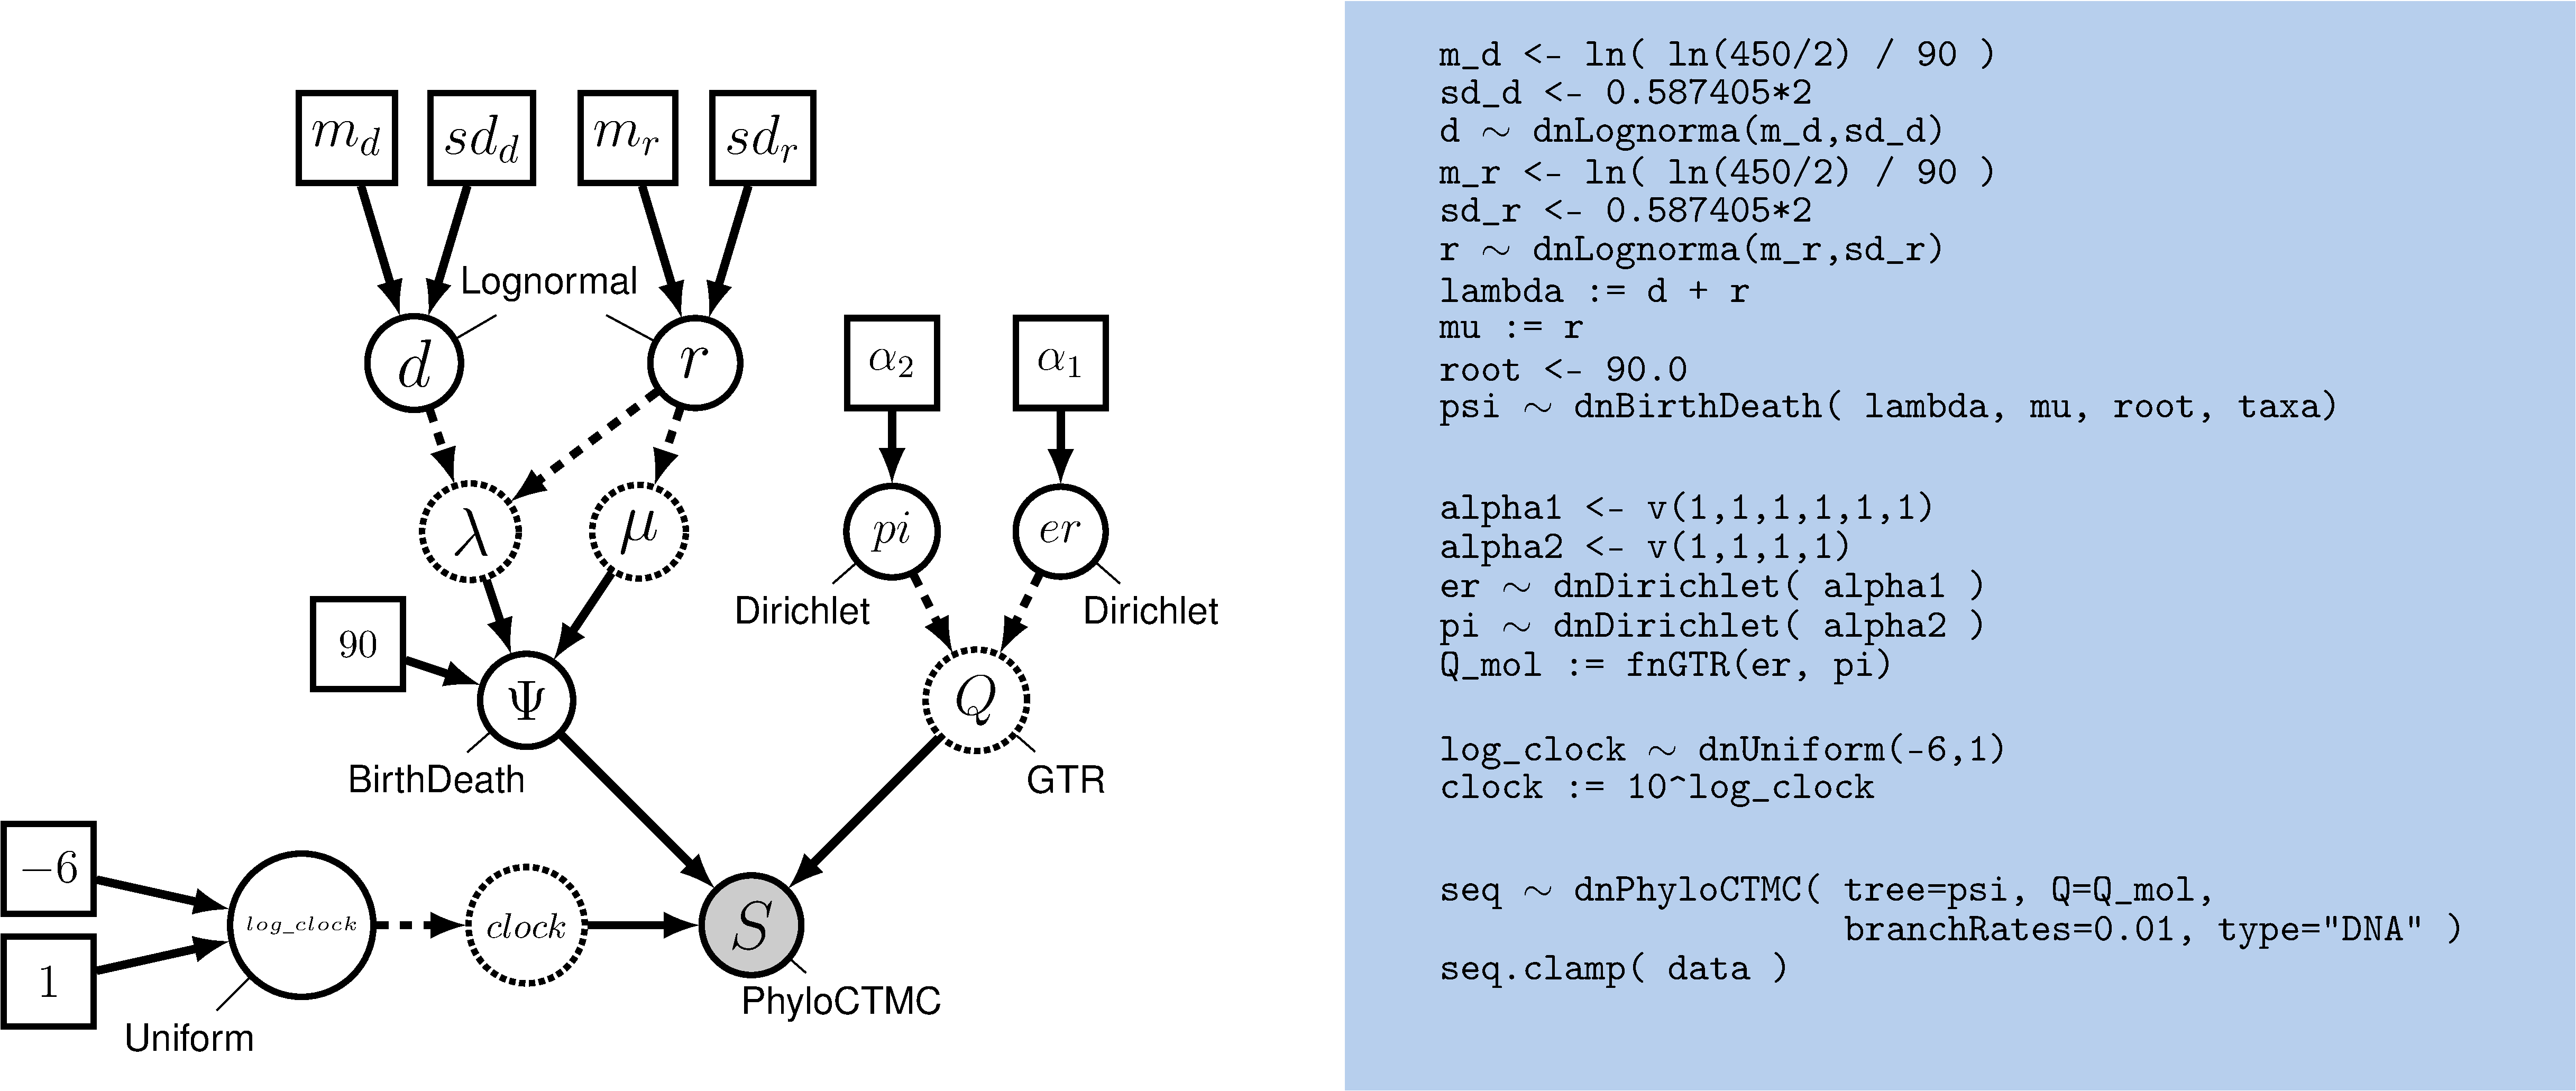
\includegraphics[width=\textwidth,angle=0]{\ResourcePath figures/gtr_graphical_model.pdf}}
\caption{\small Graphical model representation of the General Time Reversible (GTR) phylogenetic model.}
\label{fig:gtr}
\end{figure}

The GTR model requires that we define and specify a prior on the six exchangeability rates, which we will describe using a flat Dirichlet distribution.
As we did previously for the Dirichlet prior on base frequencies, we first define a constant node specifying the vector of concentration-parameter values using the \cl{v()} function:
{\tt \begin{snugshade*}
\begin{lstlisting}
er_prior <- v(1,1,1,1,1,1) 
\end{lstlisting}
\end{snugshade*}}
This node defines the concentration-parameter values of the Dirichlet prior distribution on the exchangeability rates. 
Now, we can create a stochastic node for the exchangeability rates using the \cl{dnDirichlet()} function, which takes the vector of concentration-parameter values as an argument and the \cl{\rbdn} operator. 
Together, these create a stochastic node named \cl{er} ($\theta$ in Figure \ref{fig:gtr}): 
{\tt \begin{snugshade*}
\begin{lstlisting}
er ~ dnDirichlet(er_prior)
\end{lstlisting}
\end{snugshade*}}


The Dirichlet distribution assigns probability densities to a group of parameters: e.g., those that measure proportions and must sum to 1. 
Here, we have specified a six-parameter Dirichlet prior, where each value describes one of the six relative rates of the GTR model: 
(1) $A\leftrightarrows C$; (2) $A\leftrightarrows G$; (3) $A\leftrightarrows T$; (4) $C\leftrightarrows G$; (5) $C\leftrightarrows T$; (6) $G\leftrightarrows T$. 
The input parameters of a Dirichlet distribution are called shape (or concentration) parameters. 
The expectation and variance for each variable are related to the sum of the shape parameters.
The prior we specified above is a `flat' or symmetric Dirichlet distribution; all of the shape parameters are equal (1,1,1,1,1,1).
This describes a model that allows for equal rates of change between nucleotides, such that the expected rate for each is equal to $\frac{1}{6}$ (Figure \ref{dirichletFig}a).
We might also parameterize the Dirichlet distribution such that all of the shape parameters were equal to 100, which would also specify a prior with an expectation of equal exchangeability rates (Figure \ref{dirichletFig}b). 
However, by increasing the values of the shape parameters, \cl{er\_prior <- v(100,100,100,100,100,100)}, the Dirichlet distribution will more strongly favor equal exchangeability rates; ({\it i.e.}, providing is a relatively {\em informative} prior). 
Alternatively, we might consider an asymmetric Dirichlet parameterization that could reflect a strong prior belief that transition and transversion substitutions occur at different rates.
For example, we might specify the prior density \cl{er\_prior <- v(4,8,4,4,8,4)}.   
Under this model, the expected rate for transversions would be $\frac{4}{32}$ and that for transitions would be $\frac{8}{32}$, and there would be greater prior probability on sets of GTR rates that matched this configuration (Figure \ref{dirichletFig}c). 
Yet another aymmetric prior could specify that each of the six GTR rates had a different value conforming to a Dirichlet(2,4,6,8,10,12). 
This would lead to a different prior probability density for each rate parameter (Figure \ref{dirichletFig}d).
Without strong prior knowledge about the pattern of relative rates, however, we can better reflect our uncertainty by using a vague prior on the GTR rates. 
Notably, all patterns of relative rates have the same probability density under \cl{er\_prior <- v(1,1,1,1,1,1)}.
\begin{figure}[h!]
\centering
\fbox{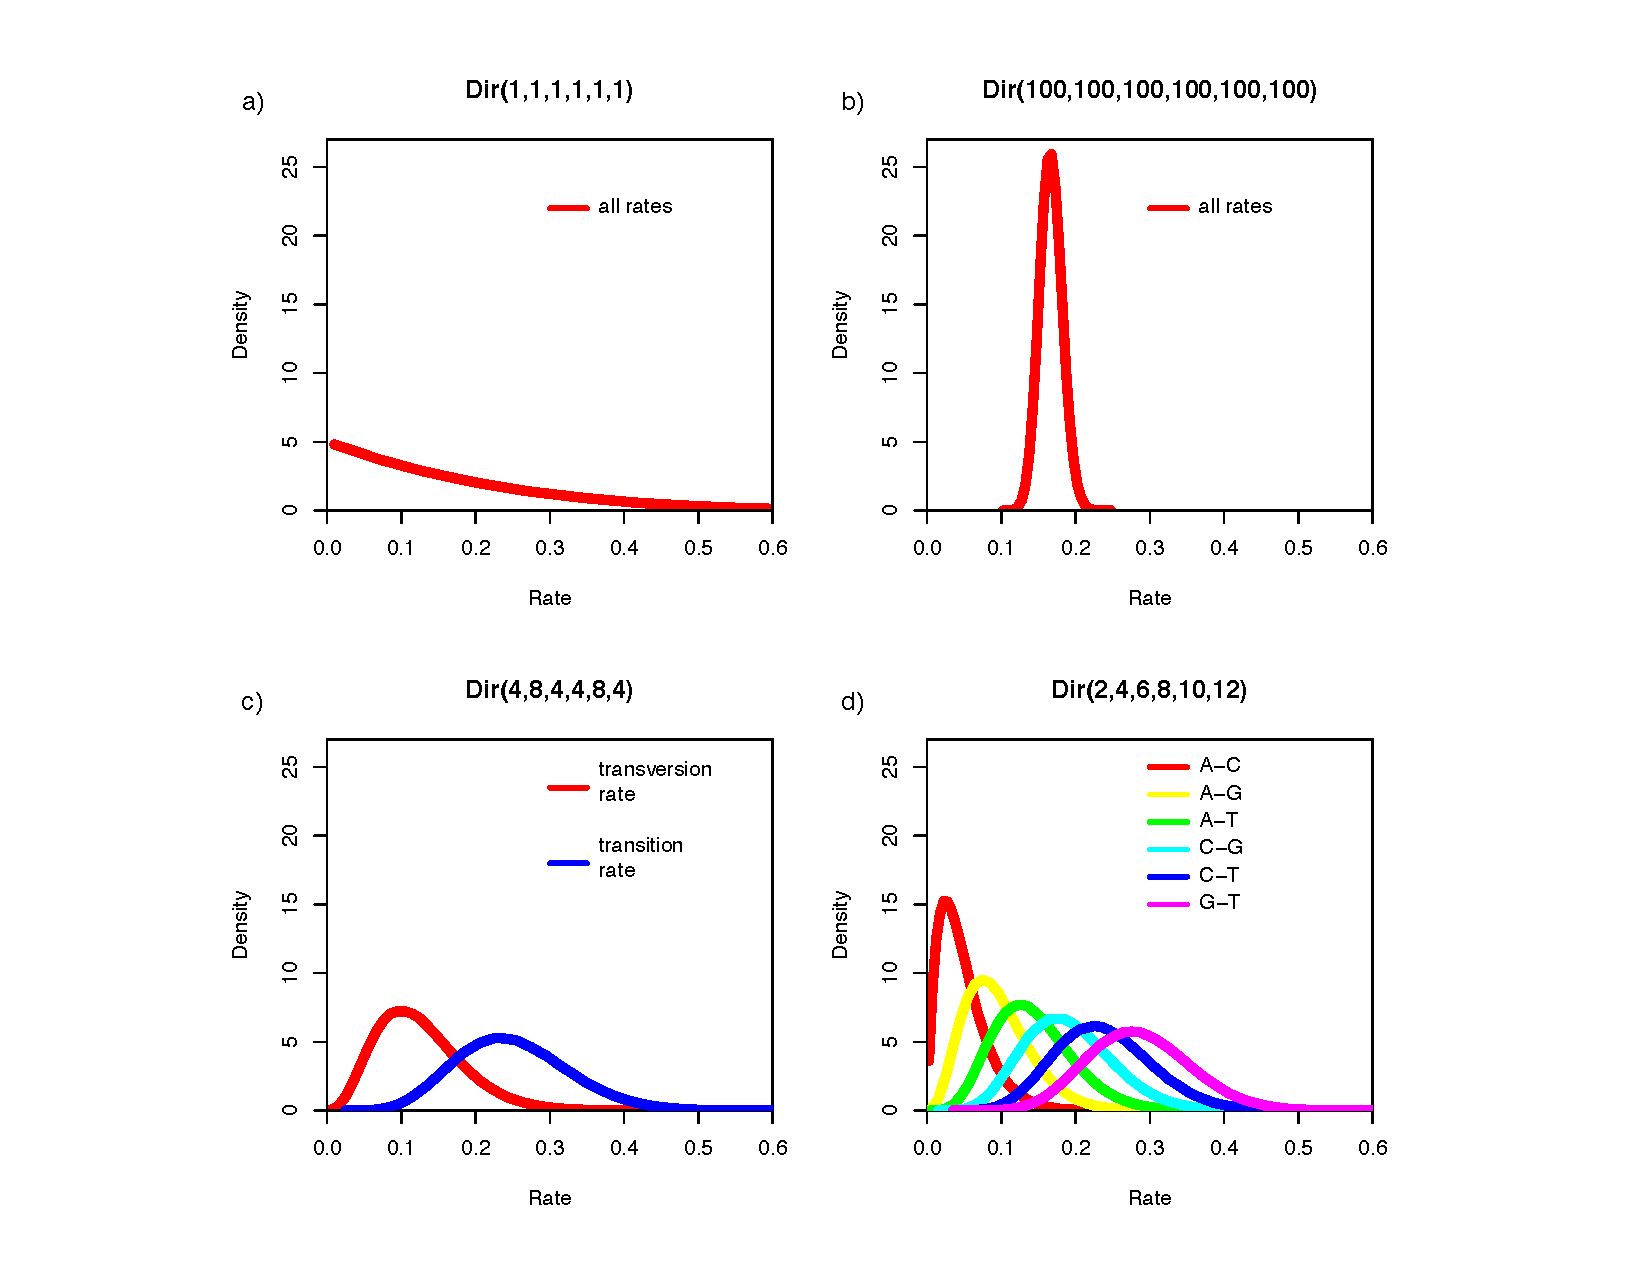
\includegraphics[width=5in]{\ResourcePath figures/dirichlet_rates.pdf}}
\caption{\small Four different examples of Dirichlet priors on exchangeability rates.}
\label{dirichletFig}
\end{figure}


For each stochastic node in our model, we must also specify a proposal mechanism if we wish to estimate that parameter. 
The Dirichlet prior on our parameter \cl{er} creates a \href{http://en.wikipedia.org/wiki/Simplex}{\textit{simplex}} of values that sum to 1. 

{\tt\small \begin{snugshade*}
\begin{lstlisting}
moves[++mvi] = mvBetaSimplex(er, weight=3)
moves[++mvi] = mvDirichletSimplex(er, weight=1)
\end{lstlisting}
\end{snugshade*}}

We can use the same type of distribution as a prior on the 4 stationary frequencies ($\pi_A, \pi_C, \pi_G, \pi_T$) since these parameters also represent proportions. 
Specify a flat Dirichlet prior density on the base frequencies:
{\tt \begin{snugshade*}
\begin{lstlisting}
pi_prior <- v(1,1,1,1) 
pi ~ dnDirichlet(pi_prior)
\end{lstlisting}
\end{snugshade*}}

The node \cl{pi} represents the $\pi$ node in Figure \ref{fig:gtr}.
Now add the simplex scale move on the stationary frequencies to the moves vector:
{\tt \small \begin{snugshade*}
\begin{lstlisting}
moves[++mvi] = mvBetaSimplex(pi, weight=2)
moves[++mvi] = mvDirichletSimplex(pi, weight=1)
\end{lstlisting}
\end{snugshade*}}

We can finish setting up this part of the model by creating a deterministic node for the GTR instantaneous-rate matrix \cl{Q}. 
The \cl{fnGTR()} function takes a set of exchangeability rates and a set of base frequencies to compute the instantaneous-rate matrix used when calculating the likelihood of our model.
{\tt \begin{snugshade*}
\begin{lstlisting}
Q := fnGTR(er,pi)
\end{lstlisting}
\end{snugshade*}}




\subsection{Execise 3}

\begin{itemize}
\item Use one of your previous analysis files---either the \cl{mcmc\_JC.Rev} or \cl{HKY.Rev}---to specify a GTR analysis in a new file called \cl{mcmc\_GTR.Rev}.
	Adapt the old analysis to be performed under the GTR substitution model. 
\item Run an MCMC analysis to estimate the posterior distribution.
\item Complete the table of the phylogenetic relationship of primates.
\end{itemize}






\newpage
\section{The Discrete Gamma Model of Among Site Rate Variation}


Members of the GTR family of substitution models assume that rates are homogeneous across sites, an assumption that is often violated by real data.
We can accommodate variation in substitution rate among sites (ASRV) by adopting the discrete-gamma model \citep{Yang1994a}.
This model assumes that the substitution rate at each site is a random variable that is described by a discretized gamma distribution, which has two parameters: the shape parameter, $\alpha$, and the rate parameter, $\beta$. 
In order that we can interpret the branch lengths as the expected number of substitutions per site, this model assumes that the mean site rate is equal to 1.
The mean of the gamma is equal to $\alpha/\beta$, so a mean-one gamma is specified by setting the two parameters to be equal, $\alpha=\beta$.
This means that we can fully describe the gamma distribution with the single shape parameter, $\alpha$. 
The degree of among-site substitution rate variation is inversely proportional to the value of the $\alpha$-shape parameter.
As the value of the $\alpha$-shape increases, the gamma distribution increasingly resembles a normal distribution with decreasing variance, which therefore corresponds to decreasing levels of ASRV (Figure \ref{asrhGammaFig}).
By contrast, when the value of the $\alpha$-shape parameter is $< 1$, the gamma distribution assumes a concave distribution that concentrates most of the prior density on low rates, but retains some prior mass on sites with very high rates, which therefore corresponds to high levels of ASRV (Figure \ref{asrhGammaFig}).
Note that, when $\alpha = 1$, the gamma distribution collapses to an exponential distribution with a rate parameter equal to $\beta$.


\begin{figure}[h]
\centering
\fbox{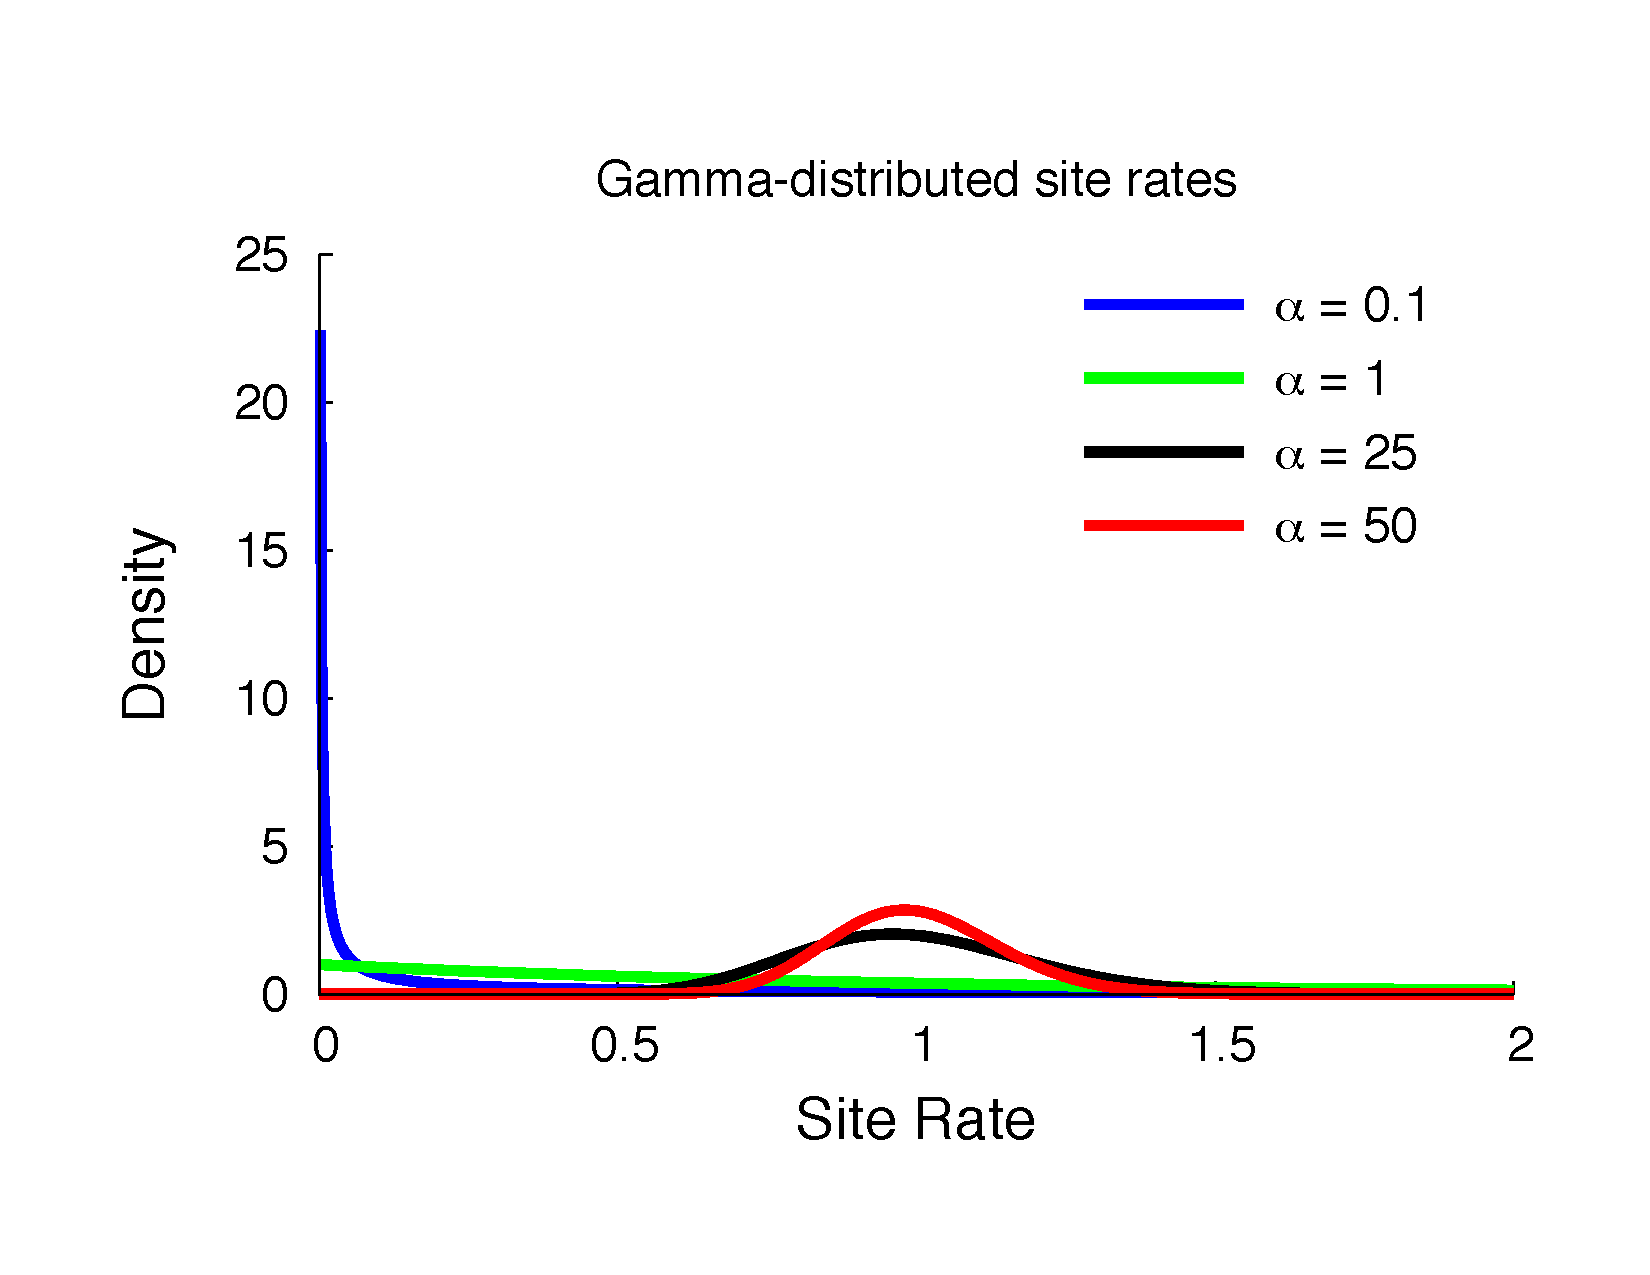
\includegraphics[width=3.5in]{\ResourcePath figures/asrh_gamma.pdf}}
\caption{\small The probability density of mean-one gamma-distributed rates for different values of the $\alpha$-shape parameter.}
\label{asrhGammaFig}
\end{figure}

We typically lack prior knowledge regarding the degree of ASRV for a given alignment.
Accordingly, rather than specifying a precise value of $\alpha$, we can instead estimate the value of the $\alpha$-shape parameter from the data.
This requires that we specify a diffuse (relatively `uninformative') prior on the $\alpha$-shape parameter.
For this analysis, we will use a lognormal distribution with a mean parameter, \cl{alpha\_prior\_mean}, equal to \cl{5.0}, and standard deviation, \cl{alpha\_prior\_sd}, equal to 0.587405 (thus, 95\% of the prior density spans exactly one order of magnitude).

This approach for accommodating ASRV is another example of a hierarchical model (Figure \ref{fig:gtrg}).
That is, variation in substitution rates across sites is addressed by applying a site-specific rate multiplier to each of the $j$ sites, $r_j$.
These rate-multipliers are drawn from a discrete, mean-one gamma distribution; the shape of this prior distribution (and the corresponding degree of ASRV) is governed by the $\alpha$-shape parameter.
The $\alpha$-shape parameter, in turn, is treated as a lognormal distributed random variable.
Finally, the shape of the lognormal prior is governed by the mean and standard deviation parameters, which are set to fixed values.   

\begin{figure}[h!]
\centering
\fbox{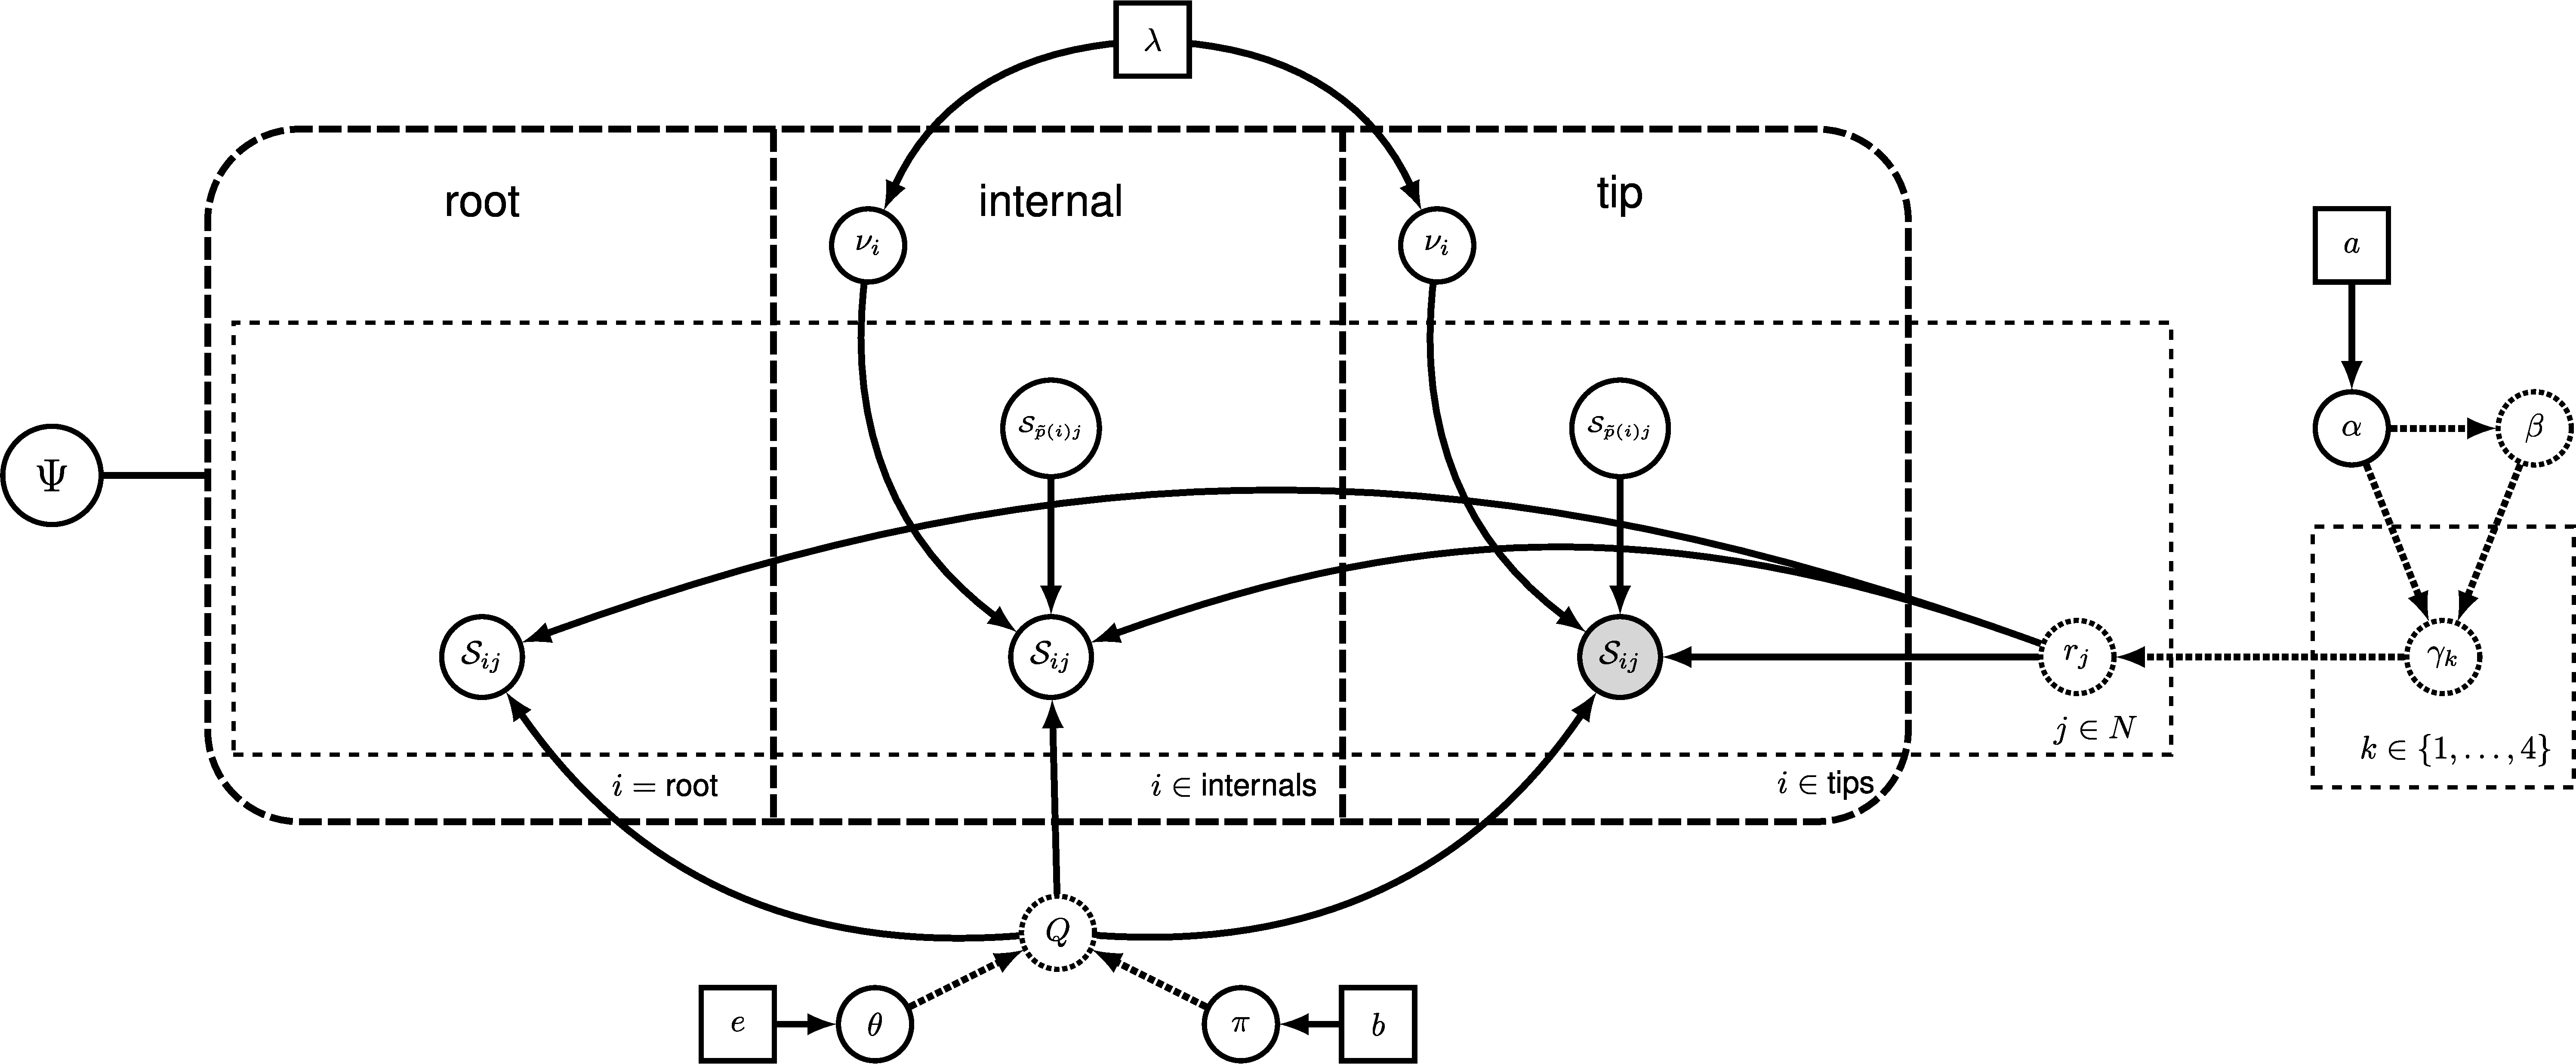
\includegraphics[width=\textwidth,angle=0]{\ResourcePath figures/gtrg_graphical_model.pdf}}
\caption{\small Graphical model representation of the General Time Reversible (GTR) + Gamma phylogenetic model.}
\label{fig:gtrg}
\end{figure}

\subsection{Setting up the Gamma Model in \RevBayes}

Create a constant node called \cl{alpha\_prior\_mean} for the mean parameter and a constant node called \cl{alpha\_prior\_sd} for the standard deviation of the lognormal prior on the gamma-shape parameter (this is represented as the constant $m_\alpha$ and $sd_\alpha$ parameters in Figure \ref{fig:gtrg}):
{\tt\begin{snugshade*}
\begin{lstlisting}
alpha_prior_mean <- ln(5.0)
alpha_prior_sd <- 0.587405
\end{lstlisting}
\end{snugshade*}}

Then create a stochastic node called \cl{alpha} with a lognormal prior (this represents the stochastic node for the $\alpha$-shape parameter in Figure \ref{fig:gtrg}):
{\tt\begin{snugshade*}
\begin{lstlisting}
alpha ~ dnLognormal( alpha_prior_mean, alpha_prior_sd )
\end{lstlisting}
\end{snugshade*}}

The way the ASRV model is implemented involves discretizing the mean-one gamma distribution into a set number of rate categories, $k$. 
Thus, we can analytically marginalize over the uncertainty in the rate at each site. 
The likelihood of each site is averaged over the $k$ rate categories, where the rate multiplier is the mean (or median) of each of the discrete $k$ categories. 
To specify this, we need a deterministic node that is a vector that will hold the set of $k$ rates drawn from the gamma distribution with $k$ rate categories. 
The \cl{fnDiscretizeGamma()} function returns this deterministic node and takes three arguments: the shape and rate of the gamma distribution and the number of categories. 
Since we want to discretize a mean-one gamma distribution, we can pass in \cl{alpha} for both the shape and rate.

Initialize the \cl{gamma\_rates} deterministic node vector using the  \cl{fnDiscretizeGamma()} function with \cl{4} bins:
{\tt \begin{snugshade*}
\begin{lstlisting}
gamma_rates := fnDiscretizeGamma( alpha, alpha, 4 )
\end{lstlisting}
\end{snugshade*}}

Note that here, by convention, we set $k = 4$.
The random variable that controls the rate variation is the stochastic node \cl{alpha}. 
We will apply a simple scale move to this parameter.
{\tt \begin{snugshade*}
\begin{lstlisting}
moves[++mvi] = mvScale(alpha, weight=2.0)
\end{lstlisting}
\end{snugshade*}}

Remember that you need to call the \cl{PhyloCTMC} constructor to include the new site-rate parameter:
{\tt \begin{snugshade*}
\begin{lstlisting}
seq ~ dnPhyloCTMC(tree=psi, Q=Q, branchRates=clockRate, siteRates=gamma_rates, type="DNA")
\end{lstlisting}
\end{snugshade*}}


\subsection{Execise 4}

Modify the previous GTR analysis to specify the GTR+Gamma model. 
Run an MCMC simulation to estimate the posterior distribution.
\begin{itemize}
\item Is there an impact on the estimated phylogeny compared with the previous analyses? 
	Look at the MAP tree and the posterior probabilities of the clades.
\item Complete the table of the phylogenetic relationship of primates.
\end{itemize}



\newpage
\section{Modeling Invariable Sites}
All of the substitution models described so far assume that the sequence data are potentially variable.
That is, we assume that the sequence data are random variables; specifically, we assume that they are realizations of the specified \cl{PhyloCTMC} distribution. 
However, some sites may not be free to vary---when the substitution rate of a site is zero, it is said to be \emph{invariable}.
Invariable sites are often confused with \emph{invariant} sites---when each species exhibits the same state, it is said to be invariant.
The concepts are related but distinct.
If a site is truly invariable, it will necessarily give rise to an invariant site pattern, as such sites will always have a zero substitution rate.
However, an invariant site pattern may be achieved via multiple substitutions that happen to end in the same state for every species.

Here we describe an extension to our phylogenetic model to accommodate invariable sites.
Under the invariable-sites model \citep[][]{Hasegawa1985}, each site is invariable with probability \cl{pinvar}, and variable with probability $1-$\cl{pinvar}.

First, let's have a look at the data and see how many invariant sites we have:
{\tt \begin{snugshade*}
\begin{lstlisting}
data.getNumInvariantSites()
\end{lstlisting}
\end{snugshade*}}
There seem to be a substantial number of invariant sites.

Now let's specify the invariable-sites model in \RevBayes.
We need to specify the prior probability that a site is invariable.
A Beta distribution is a common choice for parameters representing probabilities.
{\tt \begin{snugshade*}
\begin{lstlisting}
pinvar ~ dnBeta(1,1)
\end{lstlisting}
\end{snugshade*}}
The \cl{Beta(1,1)} distribution is a flat prior distribution that specifies equal probability for all values between 0 and 1.

Then, as usual, we add a move to change this stochastic variable; we'll used a simple sliding window move.
{\tt \begin{snugshade*}
\begin{lstlisting}
moves[++mvi] = mvSlide(pinvar)
\end{lstlisting}
\end{snugshade*}}

Finally, that you need to call the \cl{PhyloCTMC} constructor to include the new\cl{pinvar} parameter:
{\tt \begin{snugshade*}
\begin{lstlisting}
seq ~ dnPhyloCTMC(tree=psi, Q=Q, branchRates=clockRate, siteRates=gamma_rates, pInv=pinvar, type="DNA")
\end{lstlisting}
\end{snugshade*}}

\subsection{Exercise 5}

\begin{itemize}
\item Extend the GTR model to account for invariable sites and run an analysis.
\item What is the estimated probability of invariable sites and how does it relate to the ratio of invariant sites to the total number of sites?
\item Extend the GTR+$\Gamma$ model to account for invariable sites and run an analysis.
\item What is the estimated probability of invariable sites now?
\item Complete the table of the phylogenetic relationship of primates.
\end{itemize} 


\bibliographystyle{sysbio}
\bibliography{\GlobalResourcePath refs}


\chapter{Data Partitioning}
\def \ResourcePath {RB_Partition_Tutorial/}
\section{Overview}

This tutorial provides the second protocol from our recent publication \citep{Hoehna2017a}.
The first protocol is described in the \href{https://github.com/revbayes/revbayes_tutorial/raw/master/tutorial_TeX/RB_CTMC_Tutorial/RB_CTMC_Tutorial.pdf}{Substitution model tutorial} and the third protocol is described in the \href{https://github.com/revbayes/revbayes_tutorial/raw/master/tutorial_TeX/RB_BayesFactor_Tutorial/RB_BayesFactor_Tutorial.pdf}{Bayes factor tutorial}.

This tutorial demonstrates how to accommodate variation in the substitution process across sites of an alignment.
In the preceding tutorials, we assumed that all sites in an alignment evolved under an identical substitution process.
This assumption is likely to be violated biologically, since different nucleotide sites are subject to different selection pressures, such as depending on which gene or codon position the site belongs to.
Here, we will demonstrate how to specify---and select among---alternative \emph{data partition schemes} using \RevBayes.
This is commonly referred to as partitioned-data analysis, where two or more subsets of sites in our alignment are assumed to evolve under distinct processes.

This tutorial will construct three multi-gene models.
The first model, Partition\_uniform, assumes all genes evolve under the same process parameters.
The second model, Partition\_gene, assumes all genes evolve according to the same process, but each gene has it's own set of process parameters.
The third model, Partition\_codon, partitions the data not only by gene, but also by codon position.
Each analysis will generate a \emph{maximum a posteriori} tree to summarize the inferred phylogeny.
An advanced exercise introduces how to compute Bayes factors to select across various partitioning schemes.

All of the files for this analysis are provided for you and you can run these without significant effort using the \cl{source()} function in the \RevBayes console, \EG
{\tt \begin{snugshade*}
\begin{lstlisting}
source("scripts/mcmc_Partition_uniform.Rev")
\end{lstlisting}
\end{snugshade*}}

If everything loaded properly, then you should see the program begin running the Markov chain Monte Carlo analysis needed for estimating the posterior distribution. 
If you continue to let this run, then you will see it output the states of the Markov chain once the MCMC analysis begins.

\subsection{Requirements}
We assume that you have read and hopefully completed the following tutorials:
\begin{itemize}
\item \href{https://github.com/revbayes/revbayes_tutorial/raw/master/tutorial_TeX/RB_Getting_Started/RB_Getting_Started.pdf}{Getting started}
\item \href{https://github.com/revbayes/revbayes_tutorial/raw/master/tutorial_TeX/RB_Basics_Tutorial/RB_Basics_Tutorial.pdf}{\Rev basics}
\item \href{https://github.com/revbayes/revbayes_tutorial/raw/master/tutorial_TeX/RB_CTMC_Tutorial/RB_CTMC_Tutorial.pdf}{Substitution model}
\item \href{https://github.com/revbayes/revbayes_tutorial/raw/master/tutorial_TeX/RB_BayesFactor_Tutorial/RB_BayesFactor_Tutorial.pdf}{Model selection using Bayes factors}
\end{itemize}
Note that the \href{https://github.com/revbayes/revbayes_tutorial/raw/master/tutorial_TeX/RB_Basics_Tutorial/RB_Basics_Tutorial.pdf}{\Rev basics tutorial} introduces the basic syntax of \Rev but does not cover any phylogenetic models.
You may skip the \href{https://github.com/revbayes/revbayes_tutorial/raw/master/tutorial_TeX/RB_Basics_Tutorial/RB_Basics_Tutorial.pdf}{\Rev basics tutorial} if you have some familiarity with \R.
We tried to keep this tutorial very basic and introduce all the language concepts and theory on the way.
You may only need the \href{https://github.com/revbayes/revbayes_tutorial/raw/master/tutorial_TeX/RB_Basics_Tutorial/RB_Basics_Tutorial.pdf}{\Rev basics tutorial} for a more in-depth discussion of concepts in \Rev.



%%%%%%%%
%%   Data   %%
%%%%%%%%
\section{Data and files}

We provide several data files that we will use in this tutorial; these are the same datasets that we have used in previous tutorials.
In the \cl{data} folder, you will find the following files
\begin{itemize}
\item
\cl{primates\_cytb.nex}: Alignment of the \textit{cytochrome b} subunit from 23 primates representing 14 of the 16 families (\textit{Indriidae} and \textit{Callitrichidae} are missing).
\item
\cl{primates\_cox2.nex}: Alignment of the \textit{COX-II} gene from the same 23 primates species.
\end{itemize}



\section{Introduction \& Background}

Variation in the evolutionary process across the sites of nucleotide sequence alignments is well established, and is an increasingly pervasive feature of datasets composed of gene regions sampled from multiple loci and/or different genomes.
Inference of phylogeny from these data demands that we adequately model the underlying process heterogeneity; failure to do so can lead to biased estimates of phylogeny and other parameters \citep{Brown2007}.

Accounting for process heterogeneity involves adopting a partitioned data approach (sometimes also called a `mixed-model' approach \citep{Ronquist2003}), in which the sequence alignment is first parsed into a number of data subsets that are intended to capture plausible process heterogeneity within the data.
The determination of the partitioning scheme is guided by biological considerations regarding the dataset at hand.
For example, we might wish to evaluate possible variation in the evolutionary process within a single gene region (\EG between stem and loop regions of ribosomal sequences), or among gene regions in a concatenated alignment (\EG comprising multiple nuclear loci and/or gene regions sampled from different genomes).
The choice of partitioning scheme is up to the investigator and many possible partitions might be considered for a typical dataset.

In this exercise, we assume that each data subset evolved under an independent general-time reversible model with gamma-distributed rates across sites (GTR+$\Gamma$). 
Under this model the observed data are conditionally dependent on the exchangeability rates ($\theta$), stationary base frequencies ($\pi$), and the degree of gamma-distributed among-site rate variation ($\alpha$), as well as the rooted tree ($\Psi$) and branch lengths.
We show the graphical model representation of the GTR+$\Gamma$ mode in Figure \ref{fig:pipeline}. 
When we assume different GTR+$\Gamma$ models for each data subset, this results in a composite model, in which all sites are assumed to share a common, rooted tree topology and proportional branch lengths, but subsets of sites are assumed to have independent substitution model parameters.
Finally, we perform a separate MCMC simulation to approximate the joint posterior probability density of the phylogeny and other parameters. 

For most sequence alignments, several (possibly many) partition schemes of varying complexity are plausible \emph{a priori}, which therefore requires a way to objectively identify the partition scheme that balances estimation bias and error variance associated with under- and over-parameterized mixed models, respectively.
Increasingly, partition-model selection is based on \textit{Bayes factors} \citep[\EG][]{Suchard2001}, which involves first calculating the marginal likelihood under each candidate partition scheme and then comparing the ratio of the marginal likelihoods for the set of candidate partition schemes \citep{Brandley2005,Nylander2004,Mcguire2007}.
The analysis pipeline that we will use in this tutorial is depicted in Figure \ref{fig:pipeline}.

\begin{figure}[ht!]
\centering
\fbox{\includegraphics[width=6.8in,angle=0]{\ResourcePath figures/pipeline.eps}}
\caption{\small The analysis pipeline for Exercise 1. We will explore three partition schemes for the primates dataset.
The first model (the `uniform model', $M_0$) assumes that all sites evolved under a common GTR+$\Gamma$ substitution model.
The second model (the `moderately partitioned' model, $M_1$) invokes two data subsets corresponding to the two gene regions (cytB and cox2), and assumes each subset of sites evolved under an independent GTR+$\Gamma$ model.
The final partition model (the `highly partitioned' model, $M_2$) invokes four data subsets---the first two subsets corresponds to the cytB gene region, where the first and second codon position sites are combined into one subset distinct from the third codon position sites, and the cox2 has two subsets of its own, partitioned by codon positions in the same way---and each data subset is assumed evolved under an independent GTR+$\Gamma$ substitution model.
Note that we assume that all sites share a common tree topology, $\Psi$, and branch-length proportions, for each of the candidate partition schemes.
We perform two separate sets of analyses for each partition model---a MCMC simulation to approximate the joint posterior probability density of the partition-model parameters, and a `power-posterior' MCMC simulation to approximate the marginal likelihood for each mixed model.
The resulting marginal-likelihood estimates are then evaluated using Bayes factors to assess the fit of the data to the three candidate partition models.  
}
\label{fig:pipeline}
\end{figure}
\newpage



\section{Concatenated, Non-partitioned}\label{sec:unif} 

Our first exercise is to construct a multi-gene analysis where all genes evolve under the same process and parameters.

\subsection{Setting up the model}

\subsubsection{Loading and preparing the data}

To begin, load in the sequences using the \cl{readDiscreteCharacterData()} function. 
{\tt \begin{snugshade*}
\begin{lstlisting}
data_cox2 = readDiscreteCharacterData("data/primates_cox2.nex")
data_cytb = readDiscreteCharacterData("data/primates_cytb.nex")
\end{lstlisting}
\end{snugshade*}}

Since the first step in this exercise is to assume a single model across genes, we need to combine the two datasets using {\tt concatenate()}

{\tt \begin{snugshade*}
\begin{lstlisting}
data = concatenate( data_cox2, data_cytb )
\end{lstlisting}
\end{snugshade*}}

Typing \cl{data} reports the dimensions of the concatenated matrix, this provides information about the alignment:


{\tt \begin{snugshade*}
\begin{lstlisting}

   DNA character matrix with 23 taxa and 1852 characters
   =====================================================
   Origination:                   primates_cox2.nex
   Number of taxa:                23
   Number of included taxa:       23
   Number of characters:          1852
   Number of included characters: 1852
   Datatype:                      DNA

\end{lstlisting}
\end{snugshade*}}

For later use, we will store the taxon information (\cl{taxa}) and the number of taxa and branches.
{\tt \begin{snugshade*}
\begin{lstlisting}
n_species <- data.ntaxa()
n_branches <- 2 * n_species - 3
taxa <- data.taxa()
\end{lstlisting}
\end{snugshade*}}

Additionally, we will create some move and monitor index variables to create our move and monitor vectors.
{\tt \begin{snugshade*}
\begin{lstlisting}
mvi = 0
mni = 0
\end{lstlisting}
\end{snugshade*}}

\subsubsection{Substitution model}

Now we can proceed with building our GTR$+\Gamma$ model.
First, we will define and specify a prior on the exchangeability rates of the GTR model

{\tt \begin{snugshade*}
\begin{lstlisting}
er_prior <- v(1,1,1,1,1,1) 
er ~ dnDirichlet( er_prior )
\end{lstlisting}
\end{snugshade*}}

and assign its moves

{\tt \begin{snugshade*}
\begin{lstlisting}
moves[++mvi] = mvBetaSimplex(er, alpha=10, tune=true, weight=3) 
moves[++mvi] = mvDirichletSimplex(er, alpha=10.0, tune=true, weight=1.0)
\end{lstlisting}
\end{snugshade*}}

We can use the same type of distribution as a prior on the 4 stationary frequencies ($\pi_A, \pi_C, \pi_G, \pi_T$) since these parameters also represent proportions. 
Specify a flat Dirichlet prior density on the base frequencies:
{\tt \begin{snugshade*}
\begin{lstlisting}
pi_prior <- v(1,1,1,1) 
pi ~ dnDirichlet( pi_prior )
\end{lstlisting}
\end{snugshade*}}

The node \cl{pi} represents the $\pi$ node in Figure \ref{pipeline}.
Now add the simplex scale move on the stationary frequencies to the moves vector

{\tt \small \begin{snugshade*}
\begin{lstlisting}
moves[++mvi] = mvBetaSimplex(pi, alpha=10, tune=true, weight=2) 
moves[++mvi] = mvDirichletSimplex(pi, alpha=10.0, tune=true, weight=1.0)
\end{lstlisting}
\end{snugshade*}}

We can finish setting up this part of the model by creating a deterministic node for the GTR rate matrix \cl{Q}. 
The \cl{fnGTR()} function takes a set of exchangeability rates and a set of base frequencies to compute the rate matrix used when calculating the likelihood of our model.
{\tt \begin{snugshade*}
\begin{lstlisting}
Q := fnGTR(er,pi)
\end{lstlisting}
\end{snugshade*}}


\subsubsection{Among site rate variation}

We will also assume that the substitution rates vary among sites according to an one-parametric gamma distribution, \IE where the shape equals the rate ($\alpha=\beta$) and thus with mean 1.0 \citep{Yang1994a}. 
Since we do not have good prior knowledge about the variance in site rates, thus we can place a relative diffuse lognormal prior on the shape parameter.
Create a constant node called \cl{alpha\_prior\_mean} for the mean parameter and a constant node called \cl{alpha\_prior\_sd} for the standard deviation of the lognormal prior on the gamma-shape parameter (this is represented as the constant $m_\alpha$ and $sd_\alpha$ parameters in Figure \ref{fig:gtrg}):
{\tt\begin{snugshade*}
\begin{lstlisting}
alpha_prior_mean <- ln(2.0)
alpha_prior_sd <- 0.587405
\end{lstlisting}
\end{snugshade*}}

Then create a stochastic node called \cl{alpha} with a lognormal prior:
{\tt\begin{snugshade*}
\begin{lstlisting}
alpha ~ dnLognormal( alpha_prior_mean, alpha_prior_sd )
\end{lstlisting}
\end{snugshade*}}

The way the ASRV model is implemented involves discretizing the mean-one gamma distribution into a set number of rate categories. 
Thus, we can analytically marginalize over the uncertainty in the rate at each site. 
To do this, we need a deterministic node that is a vector of rates calculated from the gamma distribution and the number of rate categories. 
The \cl{fnDiscretizeGamma()} function returns this deterministic node and takes three arguments: the shape and rate of the gamma distribution and the number of categories. 
Since we want to discretize a mean-one gamma distribution, we can pass in \cl{alpha} for both the shape and rate.

Initialize the \cl{gamma\_rates} deterministic node vector using the  \cl{fnDiscretizeGamma()} function with \cl{4} bins:
{\tt \begin{snugshade*}
\begin{lstlisting}
gamma_rates := fnDiscretizeGamma( alpha, alpha, 4, false )
\end{lstlisting}
\end{snugshade*}}

The random variable that controls the rate variation is the stochastic node \cl{alpha}. 
This variable is a single, real positive value (\cl{RevType = RealPos}). 
We will apply a simple scale move to this parameter.
The scale move's tuning parameter is called \cl{lambda} and this value dictates the size of the proposal.
{\tt \begin{snugshade*}
\begin{lstlisting}
moves[++mvi] = mvScale(alpha, lambda=0.1, tune=false, weight=4.0)
\end{lstlisting}
\end{snugshade*}}

\subsubsection{Invariant sites}

Invariant sites (sites that remain fixed throughout their evolutionary history) may be seen as an extreme case of among-site rate variation.
In contrast to $+ \Gamma$ models, the $+I$ model allows site some probability of having substitution rate equal to zero.
Here, we give the probability of a site being invariant with \cl{pinvar}
{\tt \begin{snugshade*}
\begin{lstlisting}
pinvar ~ dnBeta(1,1)
moves[++mvi] = mvScale(pinvar, lambda=0.1, tune=false, weight=2.0)
moves[++mvi] = mvSlide(pinvar, delta=10.0, tune=false, weight=2.0)
\end{lstlisting}
\end{snugshade*}}



\subsubsection{Tree prior}

The tree topology and branch lengths are also stochastic nodes in our model. 
In Figure \ref{pipeline}, the tree topology is denoted $\Psi$ and the length of the branch leading to node $i$ is $\nu_i$.

For simplicity, we will use the same prior distribution on the tree topology, a uniform topology prior, and branch lengths, independent exponential prior distributions, as done in the \href{https://github.com/revbayes/revbayes_tutorial/raw/master/tutorial_TeX/RB_CTMC_Tutorial/RB_CTMC_Tutorial.pdf}{substitution model tutorial}.

We will assume that all possible labeled, unrooted tree topologies have equal probability. 
This is the \cl{dnUniformTopology()} distribution in \RevBayes. 
Note that in \RevBayes it is advisable to specify the outgroup for your study system if you use an unrooted tree prior, whereas other software, \EG \MrBayes uses the first taxon in the data matrix file as the outgroup.
Specify the \cl{topology} stochastic node by passing in the tip labels \cl{names} to the \cl{dnUniformTopology()} distribution:
{\tt \begin{snugshade*}
\begin{lstlisting}
out_group = clade("Galeopterus_variegatus")
topology ~ dnUniformTopology(taxa, outgroup=out_group)
\end{lstlisting}
\end{snugshade*}}

To update the unrooted tree topology, we can use both a nearest-neighbor interchange move (\cl{mvNNI}) and a subtree-prune and regrafting move (\cl{mvSPR}). 
These moves do not have tuning parameters associated with them, thus you only need to pass in the \cl{topology} node and proposal \cl{weight}. 
{\tt \begin{snugshade*}
\begin{lstlisting}
moves[++mvi] = mvNNI(topology, weight=1.0)
moves[++mvi] = mvSPR(topology, weight=1.0)
\end{lstlisting}
\end{snugshade*}}
The weight specifies how often the move will be applied either on average per iteration or relative to all other moves.
Have a look at the \href{https://github.com/revbayes/revbayes_tutorial/raw/master/tutorial_TeX/RB_MCMC_Tutorial/RB_MCMC_Tutorial.pdf}{MCMC Diagnosis tutorial} for more details about moves and MCMC strategies (found on the \href{http://revbayes.github.io/tutorials.html}{\RevBayes~Tutorials Website}).


Next we have to create a stochastic node for each of the $2N-3$ branches in our tree (where $N=$ \cl{n\_species}). 
We can do this using a \cl{for} loop --- this is a plate in our graphical model. In this loop, we can create each of the branch-length nodes and assign each move. 
Copy this entire block of \Rev~code into the console:
{\tt \small \begin{snugshade*}
\begin{lstlisting}
for (i in 1:n_branches) {
   br_lens[i] ~ dnExponential(10.0)
   moves[++mvi] = mvScale(br_lens[i]) 
}
\end{lstlisting}
\end{snugshade*}}

It is convenient for monitoring purposes to add the tree length as deterministic variable. 
The tree length is simply the sum of all branch lengths. .
Accordingly, the tree length can be computed using the \cl{sum()} function, which calculates the sum of any vector of values.
{\tt \begin{snugshade*}
\begin{lstlisting}
TL := sum(br_lens)
\end{lstlisting}
\end{snugshade*}}


Finally, we can create a \emph{phylogram} (a phylogeny in which the branch lengths are proportional to the expected number of substitutions/site) by combining the tree topology and branch lengths.
We do this using the \cl{treeAssembly()} function, which applies the value of the $i^{th}$ member of the \cl{br\_lens} vector to the branch leading to the $i^{th}$ node in \cl{topology}. 
Thus, the \cl{phylogeny} variable is a deterministic node: 
{\tt \begin{snugshade*}
\begin{lstlisting}
phylogeny := treeAssembly(topology, br_lens)
\end{lstlisting}
\end{snugshade*}}

\impmark{Fore more information on tree priors please read the \href{https://github.com/revbayes/revbayes_tutorial/raw/master/tutorial_TeX/RB_DiversificationRate_Tutorial/RB_DiversificationRate_Tutorial.pdf}{RB\_DiversificationRate\_Tutorial}.}


\subsection{Putting it All Together}

We now have all the parameters needed to model the phylogenetic molecular substitution process

{\tt \begin{snugshade*}
\begin{lstlisting}
phyloSeq ~ dnPhyloCTMC(tree=psi, Q=Q,  siteRates=gamma_rates, pInv=pinvar, type="DNA")
\end{lstlisting}
\end{snugshade*}}

To compute the likelihood, we condition the process on the data observed at the tips of the tree

{\tt \begin{snugshade*}
\begin{lstlisting}
phyloSeq.clamp(data)
\end{lstlisting}
\end{snugshade*}}

Since the model is now specified, we wrap the components in a {\tt Model} object.

{\tt \begin{snugshade*}
\begin{lstlisting}
mymodel = model(Q)
\end{lstlisting}
\end{snugshade*}}


\subsubsection{Specifying Monitors}

For our MCMC analysis we need to set up a vector of \textit{monitors} to save the states of our Markov chain. 
The monitor functions are all called \cl{mn*}, where \cl{*} is the wildcard representing the monitor type.
First, we will initialize the model monitor using the \cl{mnModel} function. This creates a new monitor variable that will output the states for all model parameters when passed into a MCMC function. 
{\tt \begin{snugshade*}
\begin{lstlisting}
monitors[++mni] = mnModel(filename="output/PS_uniform.log",printgen=10)
\end{lstlisting}
\end{snugshade*}}

The \cl{mnFile} monitor will record the states for only the parameters passed in as arguments. We use this monitor to specify the output for our sampled trees and branch lengths.

{\tt \begin{snugshade*}
\begin{lstlisting}
monitors[++mni] = mnFile(psi, filename="output/PS_uniform.trees", printgen=10)
\end{lstlisting}
\end{snugshade*}}

Finally, create a screen monitor that will report the states of specified variables to the screen with \cl{mnScreen}:
{\tt \begin{snugshade*}
\begin{lstlisting}
monitors[++mni] = mnScreen(alpha, pinvar, TL, printgen=1000)
\end{lstlisting}
\end{snugshade*}}


\subsubsection{Initializing and Running the MCMC Simulation}

With a fully specified model, a set of monitors, and a set of moves, we can now set up the MCMC algorithm that will sample parameter values in proportion to their posterior probability. The \cl{mcmc()} function will create our MCMC object:
{\tt \begin{snugshade*}
\begin{lstlisting}
mymcmc = mcmc(mymodel, monitors, moves, nruns=2)
\end{lstlisting}
\end{snugshade*}}
Note that this will automatically run two independent replicated MCMC simulations because we specified \cl{nruns=2}.

We can run the \cl{.burnin()} member function if we wish to pre-run the chain and discard the initial states. 
{\tt \begin{snugshade*}
\begin{lstlisting}
mymcmc.burnin(generations=10000,tuningInterval=100)
\end{lstlisting}
\end{snugshade*}}


Now, run the MCMC:
{\tt \begin{snugshade*}
\begin{lstlisting}
mymcmc.run(generations=30000)
\end{lstlisting}
\end{snugshade*}}

When the analysis is complete, you will have the monitor files in your output directory.

\RevBayes~can also summarize the tree samples by reading in the tree-trace file:
{\tt \begin{snugshade*}
\begin{lstlisting}
treetrace = readTreeTrace("output/PS_uniform.trees", treetype="non-clock")
treetrace.summarize()
\end{lstlisting}
\end{snugshade*}}


The \cl{mapTree()} function will summarize the tree samples and write the maximum a posteriori tree to file:
{\tt \begin{snugshade*}
\begin{lstlisting}
map_tree = mapTree(treetrace,"output/PS_uniform_map.tre")
\end{lstlisting}
\end{snugshade*}}

This completes the uniform partition analysis.
The next two sections will implement more complex partitioning schemes in a similar manner.


\section{Partitioning by Gene Region}\label{secByGene}

The uniform model used in the previous section assumes that all sites in the alignment evolved under the same process described by a shared tree, branch length proportions, and parameters of the GTR+$\Gamma$ substitution model.
However, our alignment contains two distinct gene regions---cytB and cox2---so we may wish to explore the possibility that the substitution process differs between these two gene regions.
This requires that we first specify the data partitions corresponding to these two genes, then define an independent substitution model for each data partition. 

First, we'll clear the workspace of all declared variables
{\tt \begin{snugshade*}
\begin{lstlisting}
clear()
\end{lstlisting}
\end{snugshade*}}

Since we wish to avoid individually specifying each parameter of the GTR+$\Gamma$ model for each of our data partitions, we can \textit{loop} over our datasets and create vectors of nodes.
To do this, we begin by creating a vector of data file names:
{\tt \begin{snugshade*}
\begin{lstlisting}
filenames <- v("data/primates_cox2.nex", "data/primates_cytb.nex")
\end{lstlisting}
\end{snugshade*}}

Set a variable for the number of partitions:
{\tt \begin{snugshade*}
\begin{lstlisting}
n_data_subsets <- filenames.size()
\end{lstlisting}
\end{snugshade*}}

And create a vector of data matrices called \cl{data}:
{\tt \begin{snugshade*}
\begin{lstlisting}
for (i in 1:n_data_subsets){
   data[i] = readDiscreteCharacterData(filenames[i])
}
\end{lstlisting}
\end{snugshade*}}

Next, we can initialize some important variables. This does require, however, that both of our alignments have the same number of species and matching tip names.
{\tt \begin{snugshade*}
\begin{lstlisting}
taxa <- data[1].taxa()
\end{lstlisting}
\end{snugshade*}}

{\tt \begin{snugshade*}
\begin{lstlisting}
mvi = 0 
mni = 0
\end{lstlisting}
\end{snugshade*}}


\subsection{Specify the Parameters by Looping Over Partitions}

We can avoid creating unique names for every node in our model if we use a \cl{for} loop to iterate over our partitions. Thus, we will only have to type in our entire GTR+$\Gamma$ model parameters once. 
This will produce a vector for each of the unlinked parameters ---\EG there will be a vector of \cl{alpha} nodes where the stochastic node for the first partition (cytB) will be \cl{alpha[1]} and the stochastic node for the second partition (cox2) will be called \cl{alpha[2]}.

The script for the model, {\tt RevBayes\_scripts/mcmc\_Partition\_gene.Rev}, creates the model parameters for each partition in one large loop.
Here, we will split the loop into smaller parts to achieve the same end.

First, we will create the GTR rate matrix for partition $i$ by first creating exchangeability rates
{\tt \small \begin{snugshade*}
\begin{lstlisting}
for (i in 1:n_data_subsets) {
  er_prior[i] <- v(1,1,1,1,1,1)
  er[i] ~ dnDirichlet(er_prior[i])
  moves[++mvi] = mvBetaSimplex(er[i], alpha=10, tune=true, weight=3) 
}
\end{lstlisting}
\end{snugshade*}}

and stationary frequencies

{\tt \small \begin{snugshade*}
\begin{lstlisting}
for (i in 1:n_data_subsets) {
  pi_prior[i] <- v(1,1,1,1)
  pi[i] ~ dnDirichlet(pi_prior[i])
  moves[++mvi] = mvBetaSimplex(pi[i], alpha=10, tune=true, weight=2)
}
\end{lstlisting}
\end{snugshade*}}

then passing those parameters into a rate matrix function

{\tt \small \begin{snugshade*}
\begin{lstlisting}
for (i in 1:n_data_subsets) {
  Q[i] := fnGTR(er[i],pi[i]) 
}
\end{lstlisting}
\end{snugshade*}}

which states the rate matrix ({\tt Q[i]}) for partition $i$ is determined by the exchangeability rates ({\tt er[i]}) and stationary frequencies ({\tt pi[i]}) also defined for partition $i$.
Following this format, we construct the remaining partition parameters: the $+\Gamma$ mixture model

{\tt \small \begin{snugshade*}
\begin{lstlisting}
for (i in 1:n_data_subsets) {
    alpha_prior_mean[i] <- ln(2.0)
    alpha_prior_sd[i] <- 0.587405
    alpha[i] ~ dnLognormal( alpha_prior_mean[i], alpha_prior_sd[i] )
    gamma_rates[i] := fnDiscretizeGamma( alpha[i], alpha[i], 4, false )

    moves[++mvi] = mvScale(alpha[i],weight=2)
}
\end{lstlisting}
\end{snugshade*}}

the $+I$ invariant sites model

{\tt \small \begin{snugshade*}
\begin{lstlisting}
for (i in 1:n_data_subsets) {
  pinvar[i] ~ dnBeta(1,1)
  moves[++mvi] = mvScale(pinvar[i], lambda=0.1, tune=true, weight=2.0)
  moves[++mvi] = mvSlide(pinvar[i], delta=0.1, tune=true, weight=2.0)
}
\end{lstlisting}
\end{snugshade*}}

and the per-partition substitution rate multipliers 
{\tt \small \begin{snugshade*}
\begin{lstlisting}
# specify a rate multiplier for each partition
part_rate_mult ~ dnDirichlet( rep(1.0, n_data_subsets) )
moves[++mvi] = mvBetaSimplex(part_rate_mult, alpha=1.0, tune=true, weight=n_data_subsets)
moves[++mvi] = mvDirichletSimplex(part_rate_mult, alpha=1.0, tune=true, weight=2.0)

# note that we use here a vector multiplication, 
# i.e., multiplying each element of part_rate_mult by n_data_subsets
part_rate := part_rate_mult * n_data_subsets\end{lstlisting}
\end{snugshade*}}


\begin{framed}
\textbf{Different Substitution Models for each Gene}\\
Alternatively, we might be interested in applying different substitution models for each gene independently instead of assuming the same substitution albeit with different parameters for each gene.
In this two gene case this is rather simple to do by specifying the substitution model for each gene independently.
For many genes this might become lengthy and you might want to write a script to generate this section (note: we may provide such scripts soon).

For simplicity and sake of demonstration, we assume that the cytochrome b region evolves under a Jukes-Cantor substitution model and the COX-II gene under an HKY substitution model.
We begin with the cytochrome b gene and the Jukes-Cantor substitution model:
{\tt \small \begin{snugshade*}
\begin{lstlisting}
# specify the JC rate matrix
Q[1] <- fnJC(4)
\end{lstlisting}
\end{snugshade*}}

Second, we specify the HKY substitution model for the COX-II gene:
{\tt \begin{snugshade*}
\begin{lstlisting}
pi_prior <- v(1,1,1,1) 
pi ~ dnDirichlet(pi_prior)

# specify a move to propose updates to on pi
moves[++mvi] = mvBetaSimplex(pi, weight=2)
moves[++mvi] = mvDirichletSimplex(pi, weight=1)

# specify a lognormal distribution as the prior distribution on kappa
kappa ~ dnLognormal(0.0,1.25)

# a simple scaling move to update kappa
moves[++mvi] = mvScale(kappa)

# Finally, create the HKY rate matrix
Q[2] := fnHKY(kappa,pi)
\end{lstlisting}
\end{snugshade*}}
Note that we specified manually in this way our vector of rate matrices \cl{Q}.
We can thus specify any substitution model manually for a given gene.
We hope that this brief example conveys the idea how to specify gene-specific substitution models.
You can add rate-variation among sites and/or probabilities for a site being invariant for each gene too.
Finally, you can then either loop over all genes to create the \cl{dnPhyloCTMC} distribution (see below) if the structure of the model allows it (\IE if all models have a variable for site-rate-variation and probabilities for invariant site), or you efficiently set these variables to default values (\EG \cl{pinvar[i]=0.0} if there is no probability for a site being invariant for this gene), or you create the \cl{seq[i] $\sim$ dnPhyloCTMC(...)} manually outside a loop as well. 
\end{framed}


\subsubsection{Tree prior}

We assume that both genes evolve along the same tree.
Hence, we need to specify a random variable for our tree parameter which is the same as was specified for {\tt mcmc\_Partition\_uniform.Rev}.
{\tt \begin{snugshade*}
\begin{lstlisting}
out_group = clade("Galeopterus_variegatus")
# Prior distribution on the tree topology	
topology ~ dnUniformTopology(taxa, outgroup=out_group)
moves[++mvi] = mvNNI(topology, weight=5.0)
moves[++mvi] = mvSPR(topology, weight=1.0)

# Branch length prior
for (i in 1:n_branches) {
    bl[i] ~ dnExponential(10.0)
	moves[++mvi] = mvScale(bl[i])
}

TL := sum(bl)
	
psi := treeAssembly(topology, bl)
\end{lstlisting}
\end{snugshade*}}


\subsection{Putting it all together}

Since we have a rate matrix and a site-rate model for each partition, we must create a phylogenetic CTMC for each gene. 
Additionally, we must fix the values of these nodes by attaching their respective data matrices.
These two nodes are linked by the \cl{psi} node and their log-likelihoods are added to get the likelihood of the whole DAG.
{\tt \begin{snugshade*}
\begin{lstlisting}
for (i in 1:n_data_subsets) {
  phyloSeq[i] ~ dnPhyloCTMC(tree=psi, Q=Q[i], branchRates=part_rate_mult[i], siteRates=norm_gamma_rates[i], pInv=pinvar[i], type="DNA")
  phyloSeq[i].clamp(data[i])
}
\end{lstlisting}
\end{snugshade*}}

The remaining steps should be familiar:
wrap the model components in a model object

{\tt \begin{snugshade*}
\begin{lstlisting}
mymodel = model(psi)
\end{lstlisting}
\end{snugshade*}}

\subsection{Create monitors}

create the monitors

{\tt \begin{snugshade*}
\begin{lstlisting}
monitors[++mni] = mnModel(filename="output/PS_gene.log",printgen=10)
monitors[++mni] = mnFile(psi, filename="output/PS_gene.trees", printgen=100)
monitors[++mni] = mnScreen(TL, printgen=1000)
\end{lstlisting}
\end{snugshade*}}

configure and run the MCMC analysis

{\tt \begin{snugshade*}
\begin{lstlisting}
mymcmc = mcmc(mymodel, moves, monitors, nruns=2)
mymcmc.burnin(10000,100)
mymcmc.run(30000)
\end{lstlisting}
\end{snugshade*}}

and summarize the posterior density of trees with a MAP tree

{\tt \begin{snugshade*}
\begin{lstlisting}
treetrace = readTreeTrace("output/PS_gene.trees", treetype="non-clock")
treetrace.summarize()
mapTree(treetrace,"output/PS_gene_MAP.tre")
\end{lstlisting}
\end{snugshade*}}



\section{Partitioning by Codon Position and by Gene}\label{secExtremeP}

Because of the genetic code, we often find that different positions within a codon (first, second, and third) evolve at different rates.
Thus, using our knowledge of biological data, we can devise a third approach that further partitions our alignment. 
For this exercise, we will partition sites within the cytB and cox2 gene by codon position.

{\tt \begin{snugshade*}
\begin{lstlisting}
clear()
data_cox2 <- readDiscreteCharacterData("data/primates_cox2.nex")
data_cytb <- readDiscreteCharacterData("data/primates_cytb.nex")
\end{lstlisting}
\end{snugshade*}}

We must now add our codon-partitions to the \cl{data} vector.
The first and second elements in the {\tt data} vector will describe cytB data, and the third and fourth elements will describe cox2 data.
Moreover, the first and third elements will describe the evolutionary process for the first and second codon position sites, while the second and fourth elements describe the process for the third codon position sites alone.

We can create this by calling the helper function \cl{setCodonPartition()}, which is a member function of the data matrix. 
We are assuming that the gene is \textit{in frame}, meaning the first column in your alignment is a first codon position. 
The \cl{setCodonPartition()} function takes a single argument, the position of the alignment you wish to extract. 
It then returns every third column, starting at the index provided as an argument.

Before we can use the use the \cl{setCodonPartition()} function, we must first populate the position in the \cl{data} matrix with some sequences. 
Then we call the member function of \cl{data[1]} to exclude all but the 1$^{st}$ and 2$^{nd}$ positions for cox2.
{\tt \begin{snugshade*}
\begin{lstlisting}
data[1] <- data_cox2
data[1].setCodonPartition( v(1,2) )
\end{lstlisting}
\end{snugshade*}}

Assign the 3$^{rd}$ codon positions for cox2 to \cl{data[2]}:
{\tt \begin{snugshade*}
\begin{lstlisting}
data[2] <- data_cox2
data[2].setCodonPartition( 3 )
\end{lstlisting}
\end{snugshade*}}

Then repeat for cytB, being careful to store the subsetted data to elements 3 and 4:
{\tt \begin{snugshade*}
\begin{lstlisting}
data[3] <- data_cytb
data[3].setCodonPartition( v(1,2) )
data[4] <- data_cytb
data[4].setCodonPartition( 3 )
\end{lstlisting}
\end{snugshade*}}

Now we have a data vector containing for subset.
We can then specify the independent substitution models per data subset.
The remaining parts of the model are identical to the previous exercise where we partitioned by gene.

\impmark{Don't forget to rename the output files!}

\subsection{Exercises}
\begin{enumerate}

\item {\bf Reviewing posterior estimates.} Open the {\tt PS\_codon.log} file in \Tracer. Remember that data subsets 1 and 2 are for cox2, partitions 3 and 4 are for cytB, subsets 1 and 3 are for sites in the first and second codon positions (per gene), and subsets 2 and 4 are for sites in the third and fourth codon positions (per gene).

Aside from the tree topology and branch lengths, each data subset is modeled to have its own set of parameters.
However, the posterior estimates for some parameters appear quite similar between some pairs of subsets yet different between other pairs of subsets.
For example, {\tt part\_rate} is the per-subset substitution rate.
This clock is approximately one order of magnitude faster for partitions 2 and 4 (third codon position sites) than it is for subsets 1 and 3 (non-third codon position sites).

Identify other parameter-subset relationships like this in the posterior.
Under this model, would you consider the gene or the codon site position to hold greater influence over the site's evolutionary mode?

\item {\bf Comparison of MAP trees.} Open the three inferred MAP trees in \FigTree.
Check to enable ``Node Labels'', click ``Display'' and select ``posterior'' from the dropdown menu.
Internal nodes now report the probability of the clade appearing in the posterior density of sampled trees.
Do different models yield different tree topologies?
Generally, do complex models provide higher or lower clade support?

\item {\bf Partitioned model selection.}
Bayes factors are computed as the ratio of marginal likelihoods (see the \href{https://github.com/revbayes/revbayes_tutorial/raw/master/tutorial_TeX/RB_BayesFactor_Tutorial/RB_BayesFactor_Tutorial.pdf}{model selection using Bayes factors tutorial} for more details).
Rather than constructing the analysis with an {\tt mcmc} object, marginal likelihood computations rely on output from a {\tt powerPosterior} object.

Copy {\tt mcmc\_Partition\_uniform.Rev} to {\tt ml\_Partition\_uniform.Rev}.
In {\tt ml\_Partition\_uniform.Rev}, delete all lines after the {\tt model} function is called, so the MCMC is never run and the MAP tree is never computed.

Instead, configure and run a power posterior analysis

{\tt \begin{snugshade*}
\begin{lstlisting}
pow_p = powerPosterior(mymodel, moves, monitors, "output/model_uniform.out", cats=100)
pow_p.burnin(generations=5000,tuningInterval=200)
pow_p.run(generations=2000)
\end{lstlisting}
\end{snugshade*}}

then compute the marginal likelihood using the stepping stone sampler

{\tt \begin{snugshade*}
\begin{lstlisting}
ss = steppingStoneSampler(file="output/model_uniform.out", powerColumnName="power", likelihoodColumnName="likelihood")
ss.marginal()
\end{lstlisting}
\end{snugshade*}}

and again using the path sampler

{\tt \begin{snugshade*}
\begin{lstlisting}
ps = pathSampler(file="model_uniform.out", powerColumnName="power", likelihoodColumnName="likelihood")
ps.marginal()\end{lstlisting}
\end{snugshade*}}


%\item {\bf 4) Customized partition models (advanced).} Create the partitioned model where first, second, and third codon positions are partitioned per gene.
%The substitution parameters for each partition are independent {\it except} the first and second codon positions per gene share stationary frequencies.
%These parameters would be $\pi_{12}^{(cytB)}$, $\pi_{3}^{(cytB)}$, $\pi_{12}^{(cox2)}$, $\pi_{3}^{(cox2)}$.
%
%The easiest way to accomplish this is to copy {\tt model\_PS2.Rev} to {\tt model\_PS3.Rev} and modify the new file's contents.
%Specifically, you will need to adjust how the codon position partitions are defined to yield six (instead of four) partitions.
%When looping over partitions, you will need an if-statement to assign stationary frequencies properly.
%Take some care when applying monitors and moves to the new model.


\end{enumerate}


\bibliographystyle{sysbio}
\bibliography{\GlobalResourcePath refs}




\part{Inference}

\chapter{Markov chain Monte Carlo Algorithms}
\bigskip
\begin{center}
\textbf{\Large \color{red}This tutorial is currently under construction/revision.}
\end{center}
\bigskip



\section{Overview}


This tutorial demonstrates how to diagnose the performance of MCMC simulations, such as the output from \RevBayes.
You will create a phylogenetic model for the evolution of DNA sequences under a JC, HKY85, GTR, GTR+Gamma and GTR+Gamma+I substitution model.
For all these models you will perform an MCMC run to estimate phylogeny and other model parameters.

\subsection*{Requirements}
We assume that you have completed the following tutorials:
\begin{itemize}
\item RB\_MCMC\_Tutorial
\end{itemize}



\newpage
\FloatBarrier
\section{Exercise: Assessing Performance of MCMC Simulations}

``{\it You can never be absolutely certain that the MCMC is reliable, you can only identify when something has gone wrong.}'' Andrew Gelman

\bigskip
Model-based inference is, after all, based on the model.
Careful research means being vigilant both regarding the choice of model and rigorously assessing our ability to estimate under the chosen model. 
The first issue---model specification, which actually entails three closely related issues---is critically important for the simple reason that unbiased estimates can only be obtained under a model that provides a reasonable description of the process that gave rise to our data. 
{\it Model selection} entails assessing the {\it relative fit} of our dataset to a pool of candidate models. 
Rankings are based on model-selection methods that compare the relative fit of candidate modes based either on their maximum-likelihood estimates (which measures the fit of the data to the model at a single point in parameter space), or on marginal likelihood of the candidate models (which measures the average fit of the candidate models to the data). 
{\it Model adequacy}---an equally important but relatively neglected issue---assesses the absolute fit of the data to the model. 
{\it Model uncertainty} is related to the common (and commonly ignored) scenario when multiple candidate models provide a similar fit to the data: in this scenario, conditioning on {\it any single} model (even the best) will lead to biased estimates, and so model averaging is required to accommodate uncertainty in the choice of model.

Much less concern is given to the second aspect of model-based inference: the ability to obtain reliable estimates under the chosen model(s). 
The implicit assumption, it seems, is that if a model is implemented correctly, and if that implementation is  successfully used to obtain an estimate from a given dataset, then we must have performed valid inference under the model. 
This would be perfectly sound reasoning if inferences were based on analytical methods. 
Owing to the complexity of the models, however, it is not possible to estimate phylogenetic parameters analytically.
Instead, parameter estimates are based on numerical methods. In the case of maximum-likelihood estimation, these are typically hill-climbing algorithms that attempt to search the profile likelihood to identify the vector of point estimates of all phylogenetic model parameters that jointly maximize the likelihood of observing the data under the model. 
The reliability of these algorithms can (and should) be assessed by comparing estimates obtained from repeated analyses that are initiated from random points in parameter space. 
Because there is only one {\it maximum} likelihood estimate, the terminal values estimated by replicate runs should be identical (within the precision of computer memory).

In the Bayesian statistical framework, inferences focus on the joint posterior probability density of phylogenetic model parameters, which is approximated by Markov chain Monte Carlo (MCMC) algorithms. 
It may be comforting to know that, in theory, an {\it appropriately constructed} and {\it adequately run} MCMC simulation is guaranteed to provide an arbitrarily precise description of the joint posterior probability density. 
In practice, however, even a given MCMC algorithm that provides reliable estimates in {\it most} cases will nevertheless fail in {\it some} cases and is not guaranteed to work for any given dataset. 
This raises an obvious question: ``When do we know that an MCMC algorithm provides reliable estimates for a given empirical analyses''. The answer is simple: \emph{Never}.
%[Leaving aside, for the moment, questions regarding the definitions of an {\it appropriately constructed} and {\it adequately run} chain.] 

Fortunately, this problem is not unique to the field of phylogenetics. 
Much of Bayesian inference outside our field also relies on MCMC algorithms to approximate the joint posterior probability density of parameters: similar concerns regarding the reliability of those inferences has motivated the development of a suite of diagnostic tools to assess MCMC performance. 
The trick is learning how to use these tools effectively and rigorously, especially for analyses that entail complex phylogenetic models and/or large datasets.

\bigskip
\subsection{MCMC Basics}

The ability to rigorously diagnose MCMC performance requires familiarity with some basic concepts from probability theory (discussed last time) and a strong intuitive understanding of the underlying mechanics---we need to know how the algorithms work in order to understand when they are not working. 
In this installment we'll briefly cover the mechanics of the Metropolis Hastings MCMC algorithm.

Recall that Bayesian inference is focused on the posterior probability density of parameters.
The posterior probability of the parameters can, in principle, be solved using Bayes' theorem.
However, (most) phylogenetic problems cannot be solved analytically, owing mainly to the denominator of Bayes' theorem---the marginal likelihood requires solving multiple integrals (for all of the continuous parameters, such as branch lengths, substitution rates, stationary frequencies, etc.) for each tree, and summing over all trees.

Accordingly, Bayesian inference of phylogeny typically resorts to numerical methods that approximate the posterior probability density. 
There are many flavors of Markov chain Monte Carlo (MCMC) algorithms---Gibbs samplers, Metropolis-coupled and reversible-jump MCMC, etc.---we will consider the Metropolis Hastings (MH) algorithm because it is commonly used for phylogenetic problems, and because it is similar to many other variants (which we will cover elsewhere). 
Note that MCMC and Bayesian inference are distinct animals: they have a relationship similar to that between 'optimization algorithms' and ‘maximum-likelihood estimation.' 
Some Bayesian inference can be accomplished without MCMC algorithms, and MCMC algorithms can be used to solve problems in non-Bayesian statistical frameworks.

To introduce the MH algorithm, we will imagine a robot that is programed to explore an area. 
Specifically, the goal of our robot is to generate a topographic map of an unknown terrain. 
This terrain has a total surface area of one hectare. 
We deploy our robot by parachute at a random location within the terrain. 
We have programmed the robot with three simple rules:

\begin{enumerate}
\item{If a proposed step will take the robot uphill, it automatically takes the proposed step.}

\item{If a proposed step will take the robot downhill, it divides the elevation of the proposed location by the elevation of the current location: we call this quotient $R$. 
It then generates a uniform random number, $U[0,1]$. 
If $U<R$, the robot takes the proposed step; otherwise, it stays put.}

\item{The distribution for proposing steps is symmetrical. 
That is, the probability of proposing a step (but not necessarily accepting a proposed step) from point A to point B is equal to the probability of proposing a step from point B to point A.}
\end{enumerate}

We allow our little robot to wander through the terrain following these three simple rules. 
At prescribed intervals  ({\it e.g.}, every $10$ proposed steps), the robot records the details of his position (his elevation, latitude, longitude, etc.) in a log. 
If we allow our robot to wander long enough, his log is guaranteed to provide an arbitrarily precise description of the topography of the terrain. 

Let's consider a slightly more formal description of the Metropolis-Hastings MCMC algorithm. 
First some preliminaries. 
This algorithm entails simulating a Markov chain that has a stationary distribution that is the joint posterior probability density of phylogenetic model parameters. 
The `state' of the chain is a set of parameter values that fully specify phylogenetic model: {\it e.g.}, a tree topology, a vector of branch lengths, and a set of parameters specifying the stochastic model of trait change ({\it e.g.}, for the GTR + $\Gamma$ substitution model, this comprises a vector of values for the four stationary frequencies, a vector of values for the six exchangeability parameters, and the value of the alpha parameter describing the shape of the gamma-distributed among-site rate variation). 
Under the robot analogy, the state of the chain corresponds to a unique point in the terrain. 
The Markov property of the MCMC reflects the fact that the next state of the chain only depends on the current state of the chain, but not on previous states---that is, the past affects the future only through the present. 
The Monte Carlo aspect of the MCMC reflects the fact that it is a simulation: it is a numerical method that relies on repeated random sampling.

Now, on to the MH algorithm:

\begin{enumerate}
\item{Initialize the chain with values for all parameters, including the tree topology, $\tau$, the vector of branch lengths $\nu$, and substitution model parameters $\pi_i$, $q_i$, $\alpha$. 
We will call the set of model parameters $\theta$. The initial parameter values might be specified arbitrarily, or might be drawn from the corresponding prior probability density for each parameter.}

\item{Select a single parameter (or set of parameters) to alter according to its proposal probability. 
For example, here are the default proposal probabilities used by \MrBayes:
{\tt \scriptsize \begin{framed}
\begin{lstlisting}
      The MCMC sampler will use the following moves:
         With prob.  Chain will use move
            1.00 %   Dirichlet(Revmat)
            1.00 %   Slider(Revmat)
            1.00 %   Dirichlet(Pi)
            1.00 %   Slider(Pi)
            2.00 %   Multiplier(Alpha)
           10.00 %   ExtSPR(Tau,V)
           10.00 %   ExtTBR(Tau,V)
           10.00 %   NNI(Tau,V)
           10.00 %   ParsSPR(Tau,V)
           40.00 %   Multiplier(V)
           10.00 %   Nodeslider(V)
            4.00 %   TLMultiplier(V)
\end{lstlisting}
\end{framed}}

We can see that $\sim 1\%$ of the time ({\it i.e.}, with probability $\sim 0.01$), the MCMC will propose changes to the exchangeability (`revmat') and stationary frequency (`pi') parameters using a `Dirichlet' proposal mechanism, and an equal effort proposing changes to the same parameters using something called a `Slider' proposal mechanism.
Conversely, $\sim 10\%$ of the time ({\it i.e.}, with probability $\sim 0.1$), the MCMC will propose changes to the tree and branch lengths (`Tau and V') using the `extending SPR' proposal mechanism, and with equal probability using the `extending TBR', `extending NNI' and the `parsimony SPR' proposal mechanisms.

For the moment, we won't worry about the details of these proposal mechanisms---they basically involve different ways of `poking' the current parameter value, $\theta$, to generate a new (proposed) parameter value, $\theta ^{\prime}$. 
The important question at the moment is: Where do these proposal probabilities come from? 
The answer is: experience. 
We want to design the MCMC such that it invests effort in a given parameter in proportion to the difficulty of approximating that parameter. 
Note that the MCMC summarized above will spend $\sim 2\%$ of its time proposing changes to the exchangeability and stationary frequency parameters, but will invest $\sim 40\%$ of its time proposing changes to the topology parameter. 
Experience suggests that the tree topology is a more difficult parameter for the MCMC to approximate relative to the exchangeability and stationary frequency parameters (in fact, it appears that the developers of \verb!MrBayes! determined from their experience that the topology is $\sim 20$ times harder to approximate).}

\item{Propose a change to the selected parameter using the parameter-specific proposal
mechanism. 
Different parameters may naturally have different prior probability densities---for example, the stationary frequencies are proportions (ranging between $0$ and $1$), and so are conveniently described using a Dirichlet prior probability density, whereas the alpha-shape parameter can range between zero and infinity, so is better described using a uniform prior probability density. 
Different kinds of prior probability densities will have specific proposal mechanisms---for example, there is something called a `Dirichlet' proposal mechanism that is used to propose new values for parameters described by a Dirichlet prior, and something called a `Slider' proposal mechanism that is used to propose new values for parameters described by a uniform prior. 
(Again, we'll go into the gory details of these proposal mechanisms another time. 
The main idea for now is that the proposal mechanisms generate a new parameter value by poking the current parameter value.)

The design of proposal mechanisms is something of a dark art---trial and error are used to guide the development of mechanisms that work well. 
Nevertheless, there are basic criteria that the proposal mechanisms must meet. 
All proposal mechanisms must be:

%\begin{enumerate}
\begin{enumerate}
\item{stochastic (new parameter values must be proposed `randomly')}

\item{irreducible (all parameter values must be potentially accessible by the chain)}

\item{aperiodic (the proposal mechanism must not induce epicycles of the chain)}
%\end{enumerate}
\end{enumerate}}

\item{Calculate the probability of accepting the proposed change, $R$:

\begin{align}
R = \text{min}\Bigg[1, \underbrace{\frac{P(X \mid \theta ^{\prime})}{P(X \mid \theta )}}_{\text{likelihood ratio}} \cdot \underbrace{\frac{ P(\theta ^{\prime})}{P(\theta)}}_\text{prior ratio} \cdot \underbrace{\frac{P(\theta \mid \theta ^{\prime})}{P(\theta ^{\prime} \mid \theta)}}_\text{proposal ratio} \Bigg]
\end{align}

The acceptance probability, $R$, is either equal to one or the product of three ratios—so long as that product is less than one (because $R$ is a probability, so it cannot be greater than one). 
So, what are these three ratios?

\textbf{Likelihood ratio:} the likelihood ratio is simply the likelihood of the observations given the proposed value of the parameter, divided by the likelihood of the observations given the current value of the parameter. 
We can calculate the likelihood for any given parameterization of the phylogenetic model using the pruning (Felsenstein) algorithm.

\textbf{Prior ratio:} in Bayesian inference, each parameter is a random variable, and so is described by a prior probability density. 
Accordingly, we can `look up' (calculate) the prior probability of any specific parameter value. 
The prior ratio is simply the prior probability of the proposed and current parameter values.

\textbf{Proposal ratio:} the proposal ratio is the probability of proposing the current parameter value given the proposed parameter value, divided by the converse. 
This is also called the Hastings ratio. 
This is equivalent to the rule that forces our robot to propose steps symmetrically; {\it i.e.}, that the probability of proposing a step from point A to point B in the terrain is equal to the probability of proposing a step from point B to point A. 
For inference problems in which the dimensions of the model are static, the proposal ratio is usually equal to one (we'll discuss exceptions to this in the context of reversible-jump MCMC in a future post).

Note that if the proposal ratio is equal to one, the acceptance probability, $R$ is based only on the product of the likelihood and prior ratios. Does that ring a bell? 
[Hint: think of Bayes' theorem.] 
[Hint 2: think of the right side of Bayes' theorem.] 
[Hint 3: think of the numerator of the right side of Bayes' theorem.] 
That is, the posterior probability is proportional to the product of the likelihood and prior probability. 
Accordingly, the acceptance probability is the posterior probability of the proposed state divided by the posterior probability of the current state. 
Just as we programmed our robot, if the ratio of the proposed and current elevations (posterior probabilities) is greater than 1 ({\it i.e.}, it is an uphill step), we always accept the proposed change. 
When the ratio of the proposed and current elevations is less than 1 ({\it i.e.}, it is an downhill step), we may or may not take the proposed step (stay tuned).}


\item{Generate a uniform random number between zero and one, $U[0,1]$. If $U<R$, accept
the proposed change; otherwise, the current state of the chain becomes the next state of the chain. 
Downhill moves will be accepted `randomly' in proportion to the difference in elevation.}

\item{Repeat steps $2-5$ an `adequate' number of times.}
\end{enumerate}

\textbf{That's it!} Notice that the decision to accept or reject proposed steps in the MCMC (and thus to sample from the joint posterior probability density) is based exclusively on the likelihood and prior probability of the proposed and current states---two quantities that are easy to calculate. 
The beautiful, fantabulous achievement of the Metropolis-Hastings algorithm is the slaying of the beastly denominator of Bayes' theorem. 
Specifically, the algorithm allows us to do inference while entirely avoiding the need to calculate the (completely intractable) marginal likelihood!

Approximating the joint posterior probability density is based on samples from the MCMC: a chain following the simple rules outlined above will sample parameter values in proportion to their posterior probability. 
That is, the proportion of time that the chain spends in any particular state is a valid approximation of the posterior probability of that state ({\it e.g.}, if a clade is present in $87\%$ of the samples drawn from the chain, then the posterior probability of that clade is estimated to be $0.87$).

Why do we accept proposals to states with lower posterior probability? 
People familiar with maximum-likelihood estimation often misunderstand the purpose of accepting proposals to states with a lower posterior probability. 
In maximum-likelihood inference, the game is to simply climb relentlessly and mindlessly up the likelihood surface in search of the very tip of the globally highest peak. 
Accordingly, the only reason these zombie hill climbers might consider a downward move would be motivated by concerns that they were currently climbing up a local (rather than global) optimum. 
By contrast, Bayesians are not just interested in the elevation of the very tip of the absolute peak of the posterior probability surface, but rather are interested in exploring and estimating the entire joint posterior probability density---we want topographical map of the entire posterior probability, not the elevation of the tip of the very highest peak in parameter space.

This survey of the joint posterior probability density results in a more robust inference procedure (inferences are averaged over the joint posterior probability of all model parameters), and allows us to estimate and evaluate the marginal posterior probability density for each of the parameters (these can be viewed by querying the MCMC samples with respect to the parameter of interest---we will do this in future tutorials). 
Accordingly, it is not sufficient for the chain to reach the peak of the joint posterior probability density; we need the chain to mix over the entire stationary distribution, spending time at each location in proportion to its posterior probability.

Next to the specification of priors (which are inspired by much more philosophical considerations), performance of the MCMC algorithm used to approximate the joint posterior probability distribution is the greatest concern associated with Bayesian inference (it is certainly a more general concern, as it holds even when the priors are uncontroversial, and, in my opinion, is a more legitimate and practical concern). 
There are three closely related issues associated with MCMC performance: (1) convergence (is the robot sampling from the stationary distribution); (2) mixing (is the robot efficiently moving over the posterior probability density); and (3) adequacy (has the robot collected sufficient samples from the target distribution to describe it adequately).


\bigskip
\section{Diagnosing MCMC performance}

\subsection{Running Markov chain Monte Carlo Simulations \& Assessing Output}\label{secUnif} 


\subsubsection{Data \& Model}

This is an analysis of 13 species within the genus \emph{Fagus} (the beeches), based 
$2576$ sites sampled from one nuclear gene region (ITS) and two chloroplast gene regions
(rbcL and matK).
Here we assume a GTR+$\Gamma$+I substitution model that is uniformly shared by all sites:
we refer to this as the `uniform' partition scheme, or PS0 for short.
This is the same data and model as we used previously in the CTMC tutorial.

Look at Model file \& MCMC file in a text editor.


\subsubsection{Running MCMC}

Let us now explore the behavior of our Markov chain.
The aim here in these exercises is to visually inspect the output generated by \RevBayes.
You should look at the trace plots using \verb!Tracer!.
Watch out for badly mixing chains, poor performance of the MCMC and correlated parameter estimates.


The first analysis which we perform is specified as follows:
\begin{itemize}
\item{uniform GTR+I+G}
\item{single move per cycle}
\item{large proposal for all parameters}
\item{no-pre-burnin}
\end{itemize}
You can run this analysis directly using
{\tt \begin{snugshade*}
\begin{lstlisting}
source("RevBayes_scripts/analysis/mcmc_run1_PS0.Rev")
mymcmc.operatorSummary()
\end{lstlisting}
\end{snugshade*}}
The operator summary provides you with an overview of the moves that you have used for this MCMC run.
It tells you what the weight for each move was, the variables it has been working on, the number of times the move was used, and how often the move was accepted.
Good acceptance rates for continuous parameters are between 20\% and 60\%.
For discrete characters, such as the phylogeny, there is no rule of thumb what good acceptance is.
Instead, the acceptance rate of tree topology proposal strongly depends on the current data.

Now let us open the generated output file in \verb!Tracer!.
The file should be called output/fagus\_ps0\_posterior\_run1.log.

What you may notice is that the ESS are very low and the MCMC is mixing very poor.
This is not good. 
We'll try a new analysis but instead run multiple moves per iteration.
The new setting is:
\begin{itemize}
\item{uniform GTR+I+G}
\item{\it multiple moves per cycle}
\item{large proposal for all parameters}
\item{flat \& low proposal weights}
\item{no-pre-burnin}
\end{itemize}
You can run this analysis in \RevBayes~using
{\tt \begin{snugshade*}
\begin{lstlisting}
source("RevBayes_scripts/analysis/mcmc_run2_PS0.Rev")
mymcmc.operatorSummary()
\end{lstlisting}
\end{snugshade*}}
Look at the output in \verb!Tracer! again.
You should see that the ESS values are still very low and the chain is still not mixing well.

One issue that you see is that the probability of a site being invariant is update not often enough.
It is quite likely that our move proposed too many bad new parameters.
So let us change the window size for the sliding window move applied on the probability of invariant sites from
{\tt \begin{snugshade*}
\begin{lstlisting}
moves[mi++] <- mvSlide(pinvar, delta=10.0, tune=false, weight=1.0)
\end{lstlisting}
\end{snugshade*}}
to
{\tt \begin{snugshade*}
\begin{lstlisting}
moves[mi++] <- mvSlide(pinvar, delta=1.0, tune=false, weight=1.0)
\end{lstlisting}
\end{snugshade*}}
This will give us now the following set-up:
\begin{itemize}
\item{uniform GTR+I+G}
\item{multiple moves per cycle}
\item{\it smaller proposals for Pinv}
\item{flat \& low proposal weights}
\item{no-pre-burnin}
\end{itemize}
Run the analysis file and look how often the Sliding Move is now accepted.
{\tt \begin{snugshade*}
\begin{lstlisting}
source("RevBayes_scripts/analysis/mcmc_run3_PS0.Rev")
mymcmc.operatorSummary()
\end{lstlisting}
\end{snugshade*}}
Open the output and look at it in \verb!Tracer!.
We are now getting better ESS values and better mixing of the MCMC.

That worked quite well but it seems to be cumbersome to adjust all the tuning parameters of the moves manually.
Instead, let us allow \RevBayes~to auto-tune the moves.
Just change \cl{tune=true} for all moves where it was \cl{tune=false} before.
Now, also include a pre-burnin.
The pre-burnin runs if you say \cl{mymcmc.burnin(generations=1000,tuningInterval=100)}.
This runs a chain for 1000 iterations and updates the tuning parameters, such as the window size, so that you achieve a good acceptance rate.
That means, if previously a move accepted too few proposal it will decrease the window size.

Here is the new model set-up:
\begin{itemize}
\item{uniform GTR+I+G}
\item{multiple moves per cycle}
\item{flat \& low proposal weights}
\item{\it pre-burnin (with scale adjusted from previous)}
\end{itemize}
Run the analysis in \RevBayes:
{\tt \begin{snugshade*}
\begin{lstlisting}
source("RevBayes_scripts/analysis/mcmc_run4_PS0.Rev")
mymcmc.operatorSummary()
\end{lstlisting}
\end{snugshade*}}
Look at the output given by the operator summary.
Notice how the tuning parameters have been updated.
Also look at the output in \verb!Tracer!.
You will see that the ESS values are much better because the chain is mixing better.

In the next step we chain the proposal weights so that moves are used more often, especially for the parameters that are not mixing well.
Our new setting is:
\begin{itemize}
\item{uniform GTR+I+G}
\item{multiple moves per cycle}
\item{\it variable proposal weights}
\item{pre-burnin (with scale adjusted from previous)}
\end{itemize}
Run the \RevBayes~analysis.
{\tt \begin{snugshade*}
\begin{lstlisting}
source("RevBayes_scripts/analysis/mcmc_run5_PS0.Rev")
mymcmc.operatorSummary()
\end{lstlisting}
\end{snugshade*}}
When you look at the output you will see that it now mixing fairly well.
So let us focus on the approximated posterior distribution.
Specifically, what is the posterior mean of the tree-length (\cl{TL})?
This tree-length is surprisingly large. 
We could specify a prior distribution with a lower expectation (mean) on the tree-length.
\begin{itemize}
\item{uniform GTR+I+G}
\item{multiple moves per cycle}
\item{variable proposal weights}
\item{pre-burnin (with scale adjusted from previous)}
\item{\it branch length prior to \cl{dnExponential(20.0)} (mean 0.05)}
\end{itemize}
Run the new analysis in \RevBayes.
{\tt \begin{snugshade*}
\begin{lstlisting}
source("RevBayes_scripts/analysis/mcmc_run6_PS0.Rev")
mymcmc.operatorSummary()
\end{lstlisting}
\end{snugshade*}}
If you look at the results from this analysis, you will notice that the tree-length estimates are better.
However, if you look at the joint posterior density of the tree-length (\cl{TL}) and the probability of a site being invariant (\cl{pinvar}), then you will notice that there is a very high correlation between these two.
It seems as if our model is over-parameterized.
To resolve this issue we need to remove/fix some of our parameters.
Open the data file and look how variable each site is. What is your impression on how many sites are invariant?

We remove the gamma distributed rate variation among sites because most sites either seem to be fixed or evolve under our GTR model.
We also reset the branch length priors to \cl{dnExponential(10.0)}.
\begin{itemize}
\item{uniform GTR+I}
\item{multiple moves per cycle}
\item{variable proposal weights}
\item{pre-burnin (with scale adjusted from previous)}
\end{itemize}
Run the new script in \RevBayes.
{\tt \begin{snugshade*}
\begin{lstlisting}
source("RevBayes_scripts/analysis/mcmc_run7_PS0.Rev")
mymcmc.operatorSummary()
\end{lstlisting}
\end{snugshade*}}
Look again at output in \verb!Tracer!.
We seem to be doing a pretty good job with one chain.
This is our visual method to inspect the MCMC output. 

Next, let's compare it to the prior.
Here we want to see how much information we actually have from the data and how much our prior influenced our posterior estimates.
Run now an analysis that does not use the data.
You can do this in \RevBayes the exact same way as running an MCMC on the exact same model, you only need to call \cl{ymmcmc.run(1000,underPrior=true)}.
{\tt \begin{snugshade*}
\begin{lstlisting}
source("RevBayes_scripts/analysis/mcmc_run8_1_prior_PS0.Rev")
mymcmc.operatorSummary()
\end{lstlisting}
\end{snugshade*}}
Load both the MCMC output under the prior and the posterior into \verb!Tracer!.
Compare the approximated distributions on each parameter between both outputs.

Since we are doing fine for a single run, try multiple runs to check if the results are reproducible.
{\tt \begin{snugshade*}
\begin{lstlisting}
source("RevBayes_scripts/analysis/mcmc_run7_1_PS0.Rev")
source("RevBayes_scripts/analysis/mcmc_run7_2_PS0.Rev")
source("RevBayes_scripts/analysis/mcmc_run7_3_PS0.Rev")
\end{lstlisting}
\end{snugshade*}}
...and the prior...
{\tt \begin{snugshade*}
\begin{lstlisting}
source("RevBayes_scripts/analysis/mcmc_run8_2_prior_PS0.Rev")
source("RevBayes_scripts/analysis/mcmc_run8_3_prior_PS0.Rev")
source("RevBayes_scripts/analysis/mcmc_run8_4_prior_PS0.Rev")
\end{lstlisting}
\end{snugshade*}}



Apply multiple-run diagnostics:
\begin{itemize}
\item{PSRF}
\item{ASDSF}
\item{comparetrees}
\end{itemize}

	
	

\bigskip
\section{Semi-automatic MCMC diagnosis using bonsai}

\definecolor{shadecolor}{RGB}{183,207,237}
Diagnosing MCMC performance manually can be extremely cumbersome, especially for more complex models.
The R package bonsai performs a standard set of diagnostics on MCMC output and generates a report that highlights potentially pathological MCMC behaviors.
To use bonsai, download the package source from https://bitbucket.org/mrmay/bonsai/downloads, launch the R console, and install the package from source (making sure to install the packages that bonsai relies on as well):
{\tt \begin{snugshade*}
\begin{lstlisting}
install.packages(packages=c('coda','tools','RColorBrewer','entropy','xtable'),dependencies=TRUE)
install.packages('< path to bonsai >',repos=NULL,type='source')
library(bonsai)
\end{lstlisting}
\end{snugshade*}}

Move the output files from \texttt{run7} to the folder \verb!.../RB_MCMC_Tutorial/output/output_for_bonsai!.

Going back to the R console, provide a name for the project.
{\tt \begin{snugshade*}
\begin{lstlisting}
project <- 'Fagus run 7'
\end{lstlisting}
\end{snugshade*}}

Point bonsai at the directory where we placed our log files.
{\tt \begin{snugshade*}
\begin{lstlisting}
path <- '.../RB_MCMC_Tutorial/output/output_for_bonsai'
\end{lstlisting}
\end{snugshade*}}

Finally, we create the bonsai object and execute the \texttt{runBonsai()} function.
It will generate a report that draws your attention to potential issues.
{\tt \begin{snugshade*}
\begin{lstlisting}
fagus_proj <- bonsai(project=project,path=path)
fagus_proj$runBonsai()
\end{lstlisting}
\end{snugshade*}}

Check the flags generated by bonsai (Figure \ref{fig:flags}; your results may differ). 
Many of these flags may be innocuous; it is up to the user to decide whether a particular flag is truly problematic.
For example, a correlation between \texttt{Likelihood} and \texttt{Posterior} is not problematic; however, a significant p-value for Geweke's diagnostic for \texttt{pi[3]} indicates that this parameter has not converged to its stationary distribution.

\begin{figure}[h!]
\begin{center}
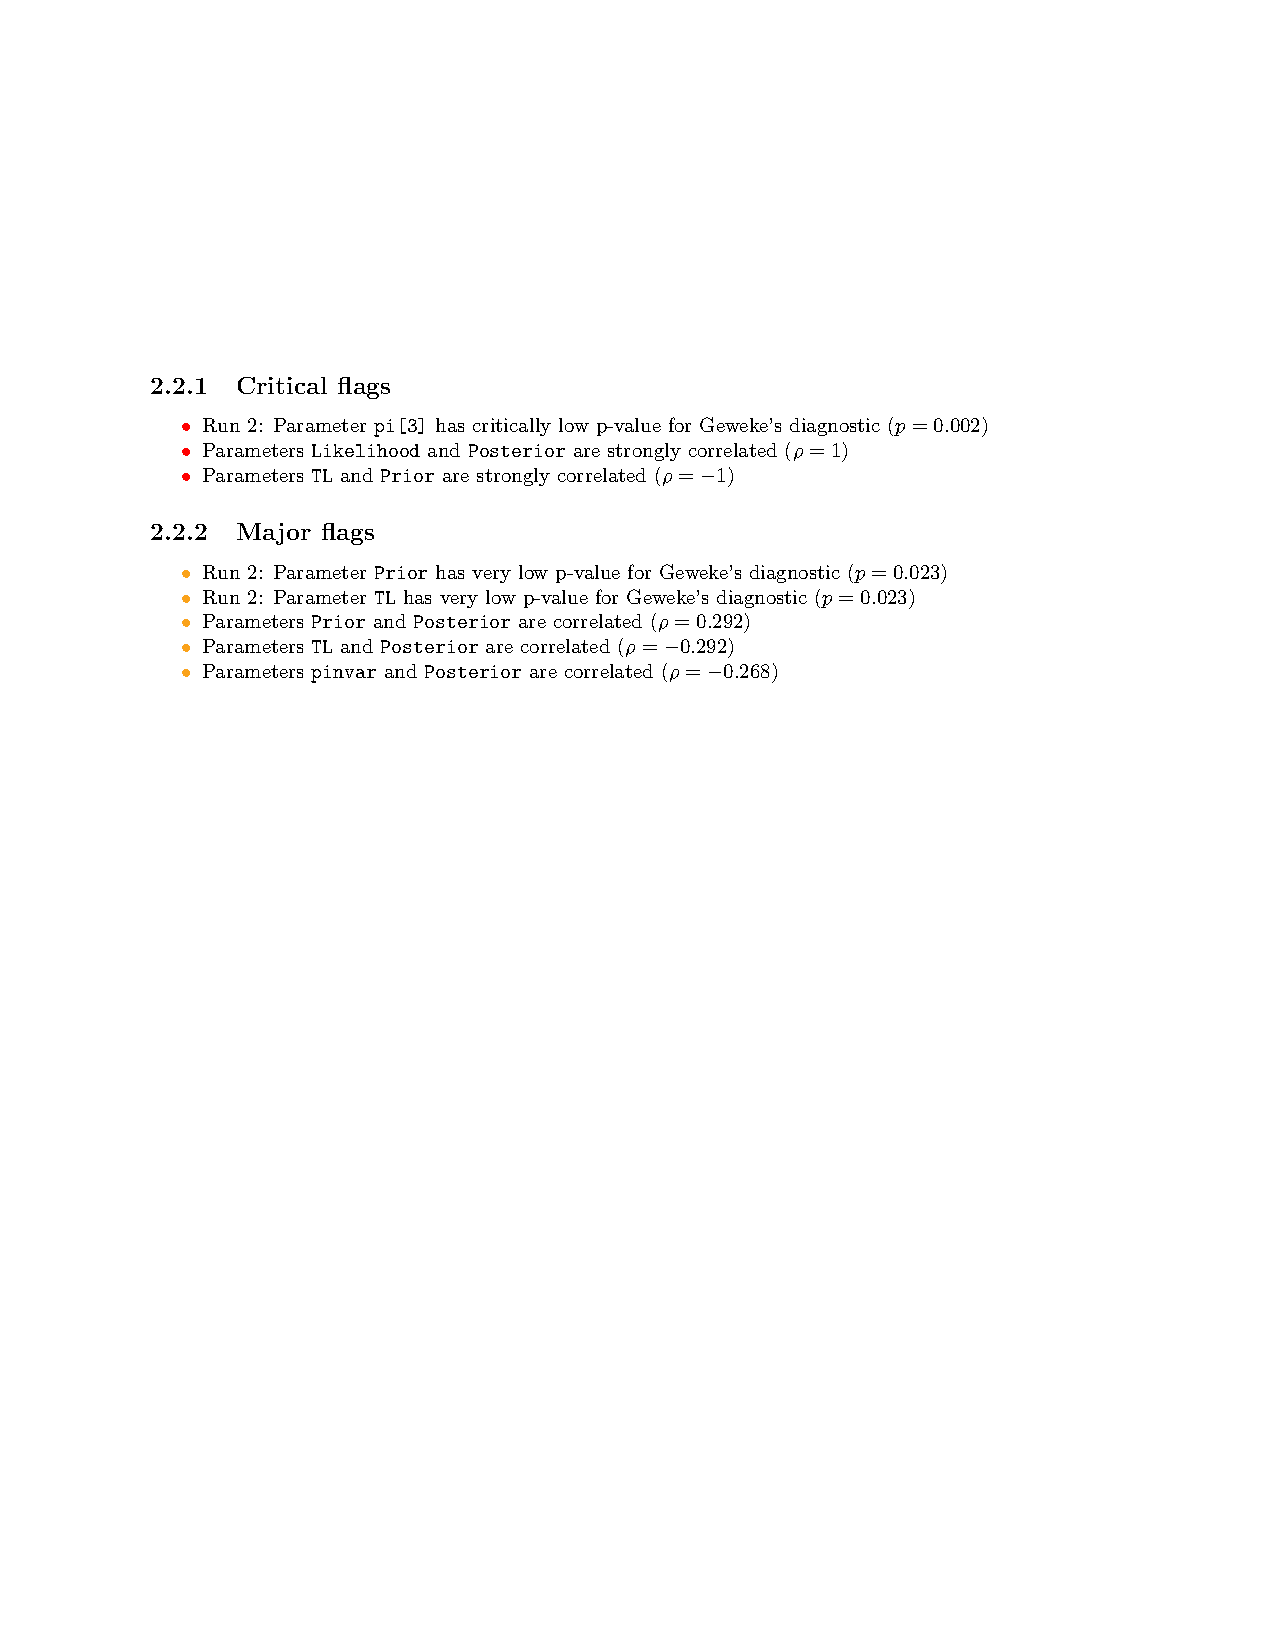
\includegraphics[]{\ResourcePath figures/flags.pdf}
\end{center}
\caption{Flags generated by bonsai.}\label{fig:flags}
\end{figure}

There are additional bonsai reports for more complex models demonstrating a wider array of MCMC pathologies in the \verb!.../RB_MCMC_Tutorial/bonsai_pre_cooked! directory.


\bibliographystyle{sysbio}
\bibliography{\GlobalResourcePath refs}


\chapter{Model Selection and Bayes Factors}
\section{Overview}


This tutorial demonstrates some general principles of Bayesian model comparison, which is based on estimating the marginal likelihood of competing models and then comparing their relative fit to the data using Bayes factors.
We consider the specific case of calculating Bayes factors to select among different substitution models.
% and different partition configurations of aligned DNA sequences. 

\subsection{Requirements}
We assume that you have read and hopefully completed the following tutorials:
\begin{itemize}
\item RB\_Getting\_Started
\item RB\_Data\_Tutorial
\item RB\_CTMC\_Tutorial
\end{itemize}
This means that we will assume that you know how to execute and load data into \RevBayes, are familiar with some basic commands, and know how to perform an analysis of a single-gene dataset (assuming an unconstrained/unrooted tree).



%%%%%%%%
%%   Data   %%
%%%%%%%%
\section{Data and files}

We provide several data files that we will use in this tutorial.
Of course, you may want to use your own dataset instead.
In the \cl{data} folder, you will find the following files
\begin{itemize}
\item
\cl{primates\_cytb.nex}: Alignment of the \textit{cytochrome b} subunit from 23 primates representing 14 of the 16 families (\textit{Indriidae} and \textit{Callitrichidae} are missing).
\item
\cl{primates\_16s.nex}: Alignment of the \textit{16s ribosomal RNA} gene from the same 23 primates species.
\item
\cl{primates\_cox2.nex}: Alignment of the \textit{COX-2} gene from the same 23 primates species.
\end{itemize}



\section{Introduction}

For most sequence alignments, several (possibly many) substitution models of varying complexity are plausible {\it a priori}.
We therefore need a way to objectively identify the model that balances estimation bias and inflated error variance associated with under- and over-parameterized models, respectively.
Increasingly, model selection is based on \textit{Bayes factors} \citep[{\it e.g.},][]{Suchard2001,Lartillot2006,Xie2011,Baele2012,Baele2013}, which involves first calculating the marginal likelihood of each candidate model and then comparing the ratio of the marginal likelihoods for the set of candidate models.

 
Given two models, $M_0$ and $M_1$, the Bayes-factor comparison assessing the relative fit of each model to the data, $BF(M_0,M_1)$, is:
$$BF(M_0,M_1) = \frac{\mbox{posterior odds}}{\mbox{prior odds}}.$$
The posterior odds is the posterior probability of $M_0$ given the data, $\mathbf X$, divided by the posterior odds of $M_1$ given the data:
$$\mbox{posterior odds} = \frac{\mathbb{P}(M_0 \mid \mathbf X)}{\mathbb{P}(M_1 \mid \mathbf X)},$$
and the prior odds is the prior probability of $M_0$ divided by the prior probability of $M_1$:
$$\mbox{prior odds} = \frac{\mathbb{P}(M_0)}{\mathbb{P}(M_1)}.$$
Thus, the Bayes factor measures the degree to which the data alter our belief regarding the support for $M_0$ relative to $M_1$ \citep{Lavine1999}:
\begin{align}\label{BFeq1}
BF(M_0,M_1) = \frac{\mathbb{P}(M_0 \mid \mathbf X, \theta_0)}{\mathbb{P}(M_1 \mid \mathbf X, \theta_1)} \div \frac{\mathbb{P}(M_0)}{\mathbb{P}(M_1)}. 
\end{align}
Note that interpreting Bayes factors involves some subjectivity.
That is, it is up to \textsl{you} to decide the degree of your belief in $M_0$ relative to $M_1$. 
Despite the absence of an absolutely objective model-selection threshold, we can refer to the scale \citep[outlined by][]{Jeffreys1961} that provides a ``rule-of-thumb'' for interpreting these measures (Table \ref{bftable}).
\begin{table}[h]
\centering
\caption{\small The scale for interpreting Bayes factors by Harold \citet{Jeffreys1961}.} 
\label{bftable}
\begin{tabular}{l c c c}
\hline
\multicolumn{1}{r}{{Strength of evidence}} & \multicolumn{1}{l}{\textbf{$BF(M_0, M_1)$}} & \multicolumn{1}{l}{\textbf{log($BF(M_0, M_1)$)}} &  \multicolumn{1}{l}{\textbf{$\text{log}_{10}$($BF(M_0, M_1)$)}}\\ 
\hline
Negative (supports $M_1$) & $<1$ & $<0$ & $<0$\\
Barely worth mentioning & $1$ to $3.2$ & $0$ to $1.16$ & $0$ to $0.5$\\
Substantial & $3.2$ to $10$ & $1.16$ to $2.3$ & $0.5$ to $1$ \\
Strong & $10$ to $100$ & $2.3$ to $4.6$ & $1$ to $2$ \\
Decisive& $>100$ & $>4.6$ & $>2$ \\
\hline
\multicolumn{3}{l}{{\scriptsize{For a detailed description of Bayes factors see \citet{Kass1995}}}} 
\end{tabular}
\end{table}


Unfortunately, it is generally not possible to directly calculate the posterior odds to prior odds ratio. 
However, we can further define the posterior odds ratio as:
\begin{align*}
\frac{\mathbb{P}(M_0 \mid \mathbf X)}{\mathbb{P}(M_1 \mid \mathbf X)} = \frac{\mathbb{P}(M_0)}{\mathbb{P}(M_1)} \frac{\mathbb{P}(\mathbf X \mid M_0)}{\mathbb{P}(\mathbf X \mid M_1)},
\end{align*}
where $\mathbb{P}(\mathbf X \mid M_i)$ is the \textit{marginal likelihood} of the data (this may be familiar to you as the denominator of Bayes Theorem, which is variously referred to as the \textit{model evidence} or \textit{integrated likelihood}).
Formally, the marginal likelihood is the probability of the observed data ($\mathbf X$) under a given model ($M_i$) that is averaged over all possible values of the parameters of the model ($\theta_i$) with respect to the prior density on $\theta_i$
\begin{align}\label{margeLike}
\mathbb{P}(\mathbf X \mid M_i) = \int \mathbb{P}(\mathbf X \mid \theta_i) \mathbb{P}(\theta_i)dt.
\end{align}
This makes it clear that more complex (parameter-rich) models are penalized by virtue of the associated prior: each additional parameter entails integration of the likelihood over the corresponding prior density.  
If you refer back to equation \ref{BFeq1}, you can see that, with very little algebra, the ratio of marginal likelihoods is equal to the Bayes factor:
\begin{align}\label{bfFormula}
BF(M_0,M_1) = \frac{\mathbb{P}(\mathbf X \mid M_0)}{\mathbb{P}(\mathbf X \mid M_1)} = \frac{\mathbb{P}(M_0 \mid \mathbf X, \theta_0)}{\mathbb{P}(M_1 \mid \mathbf X, \theta_1)} \div \frac{\mathbb{P}(M_0)}{\mathbb{P}(M_1)}. 
\end{align}
Therefore, we can perform a Bayes factor comparison of two models by calculating the marginal likelihood for each one. % Simple as pie, right?
Alas, exact solutions for calculating marginal likelihoods are not known for phylogenetic models (see equation \ref{margeLike}), thus we must resort to numerical integration methods to estimate or approximate these values. 
In this exercise, we will estimate the marginal likelihood for each partition scheme
using both the stepping-stone \citep{Xie2011,Fan2011} and path sampling estimators \citep{Lartillot2006, Baele2012}. 



\bigskip
\subsection{Substitution Models}\label{secUnif} 

The models we use here are equivalent to the models described in the previous exercise on substitution models (continuous time Markov models).
To specify the model please consult the previous exercise. Specifically, you will need to specify the following substitution models:
\begin{itemize}
\item Jukes-Cantor (JC) substitution model \citep[][]{Jukes1969}
\item Hasegawa-Kishino-Yano (HKY) substitution model \citep[][]{Hasegawa1985}
\item General-Time-Reversible (GTR) substitution model \citep[][]{Tavare1986}
\item Gamma (+G) model for among-site rate variation \citep[][]{yang94a}
\item Invariable-sites (+I) model \citep[][]{Hasegawa1985}
\end{itemize}


\bigskip
\subsection{Estimating the Marginal Likelihood}

We will estimate the marginal likelihood of a given model using a `stepping-stone' (or `path-sampling') algorithm.
These algorithms are similar to the familiar MCMC algorithms, which are intended to sample from (and estimate) the joint posterior probability of the model parameters.
Stepping-stone algorithms are like a series of MCMC simulations that iteratively sample from a specified number of discrete steps between the posterior and the prior probability distributions.
The basic idea is to estimate the probability of the data for all points between the posterior and the prior---effectively summing the probability of the data over the prior probability of the parameters to estimate the marginal likelihood. 
Technically, the steps correspond to a series of \cl{powerPosteriors()}: a series of numbers between 1 and 0 that are iteratively applied to the posterior.
When the posterior probability is raised to the power of 1 (typically the first stepping stone), samples are drawn from the (untransformed) posterior.
By contrast, when the posterior probability is raised to the power of 0 (typically the last stepping stone), samples are drawn from the prior.
To perform a stepping-stone simulation, we need to specify (1) the \emph{number} of stepping stones (power posteriors) that we will use to traverse the path between the posterior and the prior (e.g., we specify 50 or 100 stones), (2) the \emph{spacing} of the stones between the posterior and prior (e.g., we may specify that the stones are distributed according to a beta distribution), (3) the number of samples to (and thinning) of samples to be drawn from each stepping stone, and (4) the direction we will take (i.e., from the posterior to the prior or vice versa).

%With a fully specified model, we can set up the \cl{powerPosterior()} analysis to create a file of `powers' and likelihoods from which we can estimate the marginal likelihood using stepping-stone or path sampling. 
This method computes a vector of powers from a beta distribution, then executes an MCMC run for each power step while raising the likelihood to that power. In this implementation, the vector of powers starts with 1, sampling the likelihood close to the posterior and incrementally sampling closer and closer to the prior as the power decreases. 



%\textbf{\textit{Clear Workspace and Load the Data and Model}}

Just to be safe, it is better to clear the workspace (if you did not just restart \RevBayes)
{\tt \begin{snugshade*}
\begin{lstlisting}
clear()
\end{lstlisting}
\end{snugshade*}}

Now set up the model as in the previous exercise. You should start with the simple Jukes-Cantor substitution model. 
Setting up the model requires:
\begin{enumerate}
\item Loading the data and retrieving useful variables about the data (\EG number of sequences and taxon names).
\item Specifying the instantaneous-rate matrix of the substitution model.
\item Specifying the tree model including branch-length variables.
\item Creating a random variable for the sequences that evolved under the \cl{PhyloCTMC}.
\item Clamping the data.
\item Creating a model object.
\item Specifying the moves for parameter updates.
\end{enumerate}

The following procedure for estimating marginal likelihoods is valid for any model in \RevBayes.
You will need to repeat this later for other models.
First, we create the variable containing the power-posterior analysis. 
This requires that we provide a model and vector of moves, as well as an output file name. 
The \cl{cats} argument sets the number of stepping stones.
{\tt \begin{snugshade*}
\begin{lstlisting}
pow_p = powerPosterior(mymodel, moves, "model1.out", cats=50) 
\end{lstlisting}
\end{snugshade*}}

We can start the power-posterior analysis by first burning in the chain and and discarding the first 10000 states.  
This will help ensure that analysis starts from a region of high posterior probability, rather than from some random point.
{\tt \begin{snugshade*}
\begin{lstlisting}
pow_p.burnin(generations=10000,tuningInterval=1000)
\end{lstlisting}
\end{snugshade*}}

Now execute the run with the \cl{.run()} function:
{\tt \begin{snugshade*}
\begin{lstlisting}
pow_p.run(generations=1000)  
\end{lstlisting}
\end{snugshade*}}

Once the power posteriors have been saved to file, create a stepping stone sampler. 
This function can read any file of power posteriors and compute the marginal likelihood using stepping-stone sampling. 
{\tt \small \begin{snugshade*}
\begin{lstlisting}
ss <- steppingStoneSampler(file="model1.out", powerColumnName="power", likelihoodColumnName="likelihood")
\end{lstlisting}
\end{snugshade*}}

These commands will execute a stepping-stone simulation with 50 stepping stones, sampling 1000 states from each step. 
Compute the marginal likelihood under stepping-stone sampling using the member function \cl{marginal()} of the \cl{ss} variable and record the value in Table \ref{tab:ml_cytb}.
{\tt \begin{snugshade*}
\begin{lstlisting}
ss.marginal() 
\end{lstlisting}
\end{snugshade*}}

Path sampling is an alternative to stepping-stone sampling and also takes the same power posteriors as input. 
{\tt \small \begin{snugshade*}
\begin{lstlisting}
ps = pathSampler(file="model1.out", powerColumnName="power", likelihoodColumnName="likelihood")
\end{lstlisting}
\end{snugshade*}}

Compute the marginal likelihood under stepping-stone sampling using the member function \cl{marginal()} of the \cl{ps} variable and record the value in Table \ref{tab:ml_cytb}.
{\tt \begin{snugshade*}
\begin{lstlisting}
ps.marginal() 
\end{lstlisting}
\end{snugshade*}}

\noindent \\ \impmark As an example we provide the file \textbf{RevBayes\_scripts/marginalLikelihood\_JukesCantor.Rev}.


\subsection{Exercises}

\begin{itemize}
\item Compute the marginal likelihoods of the \textit{cytb} alignment for the following substitution models:
\begin{itemize}
\item Jukes-Cantor (JC) substitution model
\item Hasegawa-Kishino-Yano (HKY) substitution model
\item General-Time-Reversible (GTR) substitution model
\item GTR with gamma distributed-rate model (GTR+G)
\item GTR with invariable-sites model  (GTR+I)
\item GTR+I+G model
\end{itemize}
\item Enter the marginal likelihood estimate for each model in the corresponding cell of Table~\ref{tab:ml_cytb}.
\item Repeat the above marginal likelihood analyses for the \textit{mt-COX2 gene} and enter results in Table~\ref{tab:ml_cox2}.
\item Which is the best fitting substitution model?
\end{itemize}

\begin{Form}
\begin{table}[h]
\centering
\caption{\small Estimated marginal likelihoods for different substitution models for the cytb alignment$^*$.}
\begin{tabular}{l c c c c}
\hline
\multicolumn{1}{l}{\textbf{ }} &\multicolumn{1}{r}{\textbf{ }} & \multicolumn{3}{c}{\textbf{Marginal lnL estimates}} \\ 
\cline{3-5}
\multicolumn{1}{l}{\textbf{Substitution Model}} & \multicolumn{1}{r}{\hspace{3mm}} & \multicolumn{1}{c}{\textit{Stepping-stone}} & \multicolumn{1}{r}{\hspace{3mm}} & \multicolumn{1}{c}{\textit{Path sampling}} \\ 
\hline
JC ($M_1$) & \hspace{15mm} & \TextField[name=gene1_m11,backgroundcolor={.85 .85 .85},color={1 0 0},height=4ex]{}  & \hspace{15mm} & \TextField[name=gene1_m12,backgroundcolor={.85 .85 .85},color={0 0 1},height=4ex]{} \\
\hline
HKY ($M_2$) & \hspace{3mm} &\TextField[name=gene1_m21,backgroundcolor={.85 .85 .85},color={1 0 0},height=4ex]{}   & \hspace{3mm} & \TextField[name=gene1_m22,backgroundcolor={.85 .85 .85},color={0 0 1},height=4ex]{} \\
\hline
GTR ($M_3$) & \hspace{3mm} &\TextField[name=gene1_m31,backgroundcolor={.85 .85 .85},color={1 0 0},height=4ex]{}   & \hspace{3mm} & \TextField[name=gene1_m32,backgroundcolor={.85 .85 .85},color={0 0 1},height=4ex]{} \\
\hline
GTR+$\Gamma$ ($M_4$) & \hspace{3mm} & \TextField[name=gene1_m41,backgroundcolor={.85 .85 .85},color={1 0 0},height=4ex]{} & \hspace{3mm} & \TextField[name=gene1_m42,backgroundcolor={.85 .85 .85},color={0 0 1},height=4ex]{} \\
\hline
GTR+I ($M_5$) & \hspace{3mm} & \TextField[name=gene1_m51,backgroundcolor={.85 .85 .85},color={1 0 0},height=4ex]{} & \hspace{3mm} & \TextField[name=gene1_m52,backgroundcolor={.85 .85 .85},color={0 0 1},height=4ex]{} \\
\hline
GTR+$\Gamma$+I ($M_6$) & \hspace{3mm} & \TextField[name=gene1_m61,backgroundcolor={.85 .85 .85},color={1 0 0},height=4ex]{} & \hspace{3mm} & \TextField[name=gene1_m62,backgroundcolor={.85 .85 .85},color={0 0 1},height=4ex]{} \\
\hline
Any other model ($M_7$) & \hspace{3mm} & \TextField[name=gene1_m71,backgroundcolor={.85 .85 .85},color={1 0 0},height=4ex]{} & \hspace{3mm} & \TextField[name=gene1_m72,backgroundcolor={.85 .85 .85},color={0 0 1},height=4ex]{} \\
\hline
Any other model ($M_8$) & \hspace{3mm} & \TextField[name=gene1_m81,backgroundcolor={.85 .85 .85},color={1 0 0},height=4ex]{} & \hspace{3mm} & \TextField[name=gene1_m82,backgroundcolor={.85 .85 .85},color={0 0 1},height=4ex]{} \\
\hline
Any other model ($M_9$) & \hspace{3mm} & \TextField[name=gene1_m91,backgroundcolor={.85 .85 .85},color={1 0 0},height=4ex]{} & \hspace{3mm} & \TextField[name=gene1_m92,backgroundcolor={.85 .85 .85},color={0 0 1},height=4ex]{} \\
\hline
{\footnotesize{$^*$you can edit this table}}\\
\end{tabular}
\label{tab:ml_cytb}
\end{table}
\end{Form}


\begin{Form}
\begin{table}[h]
\centering
\caption{\small Estimated marginal likelihoods for different substitution models of the cox2 gene$^*$.}
\begin{tabular}{l c c c c}
\hline
\multicolumn{1}{l}{\textbf{ }} &\multicolumn{1}{r}{\textbf{ }} & \multicolumn{3}{c}{\textbf{Marginal lnL estimates}} \\ 
\cline{3-5}
\multicolumn{1}{l}{\textbf{Substitution Model}} & \multicolumn{1}{r}{\hspace{3mm}} & \multicolumn{1}{c}{\textit{Stepping-stone}} & \multicolumn{1}{r}{\hspace{3mm}} & \multicolumn{1}{c}{\textit{Path sampling}} \\ 
\hline
JC ($M_1$) & \hspace{15mm} & \TextField[name=gene2_m11,backgroundcolor={.85 .85 .85},color={1 0 0},height=4ex]{}  & \hspace{15mm} & \TextField[name=gene2_m12,backgroundcolor={.85 .85 .85},color={0 0 1},height=4ex]{} \\
\hline
HKY ($M_2$) & \hspace{3mm} &\TextField[name=gene2_m21,backgroundcolor={.85 .85 .85},color={1 0 0},height=4ex]{}   & \hspace{3mm} & \TextField[name=gene2_m22,backgroundcolor={.85 .85 .85},color={0 0 1},height=4ex]{} \\
\hline
GTR ($M_3$) & \hspace{3mm} &\TextField[name=gene2_m31,backgroundcolor={.85 .85 .85},color={1 0 0},height=4ex]{}   & \hspace{3mm} & \TextField[name=gene2_m32,backgroundcolor={.85 .85 .85},color={0 0 1},height=4ex]{} \\
\hline
GTR+$\Gamma$ ($M_4$) & \hspace{3mm} & \TextField[name=gene2_m41,backgroundcolor={.85 .85 .85},color={1 0 0},height=4ex]{} & \hspace{3mm} & \TextField[name=gene2_m42,backgroundcolor={.85 .85 .85},color={0 0 1},height=4ex]{} \\
\hline
GTR+I ($M_5$) & \hspace{3mm} & \TextField[name=gene2_m51,backgroundcolor={.85 .85 .85},color={1 0 0},height=4ex]{} & \hspace{3mm} & \TextField[name=gene2_m52,backgroundcolor={.85 .85 .85},color={0 0 1},height=4ex]{} \\
\hline
GTR+$\Gamma$+I ($M_6$) & \hspace{3mm} & \TextField[name=gene2_m61,backgroundcolor={.85 .85 .85},color={1 0 0},height=4ex]{} & \hspace{3mm} & \TextField[name=gene2_m62,backgroundcolor={.85 .85 .85},color={0 0 1},height=4ex]{} \\
\hline
Any other model ($M_7$) & \hspace{3mm} & \TextField[name=gene2_m71,backgroundcolor={.85 .85 .85},color={1 0 0},height=4ex]{} & \hspace{3mm} & \TextField[name=gene2_m72,backgroundcolor={.85 .85 .85},color={0 0 1},height=4ex]{} \\
\hline
Any other model ($M_8$) & \hspace{3mm} & \TextField[name=gene2_m81,backgroundcolor={.85 .85 .85},color={1 0 0},height=4ex]{} & \hspace{3mm} & \TextField[name=gene2_m82,backgroundcolor={.85 .85 .85},color={0 0 1},height=4ex]{} \\
\hline
Any other model ($M_9$) & \hspace{3mm} & \TextField[name=gene2_m91,backgroundcolor={.85 .85 .85},color={1 0 0},height=4ex]{} & \hspace{3mm} & \TextField[name=gene2_m92,backgroundcolor={.85 .85 .85},color={0 0 1},height=4ex]{} \\
\hline
{\footnotesize{$^*$you can edit this table}}\\
\end{tabular}
\label{tab:ml_cox2}
\end{table}
\end{Form}





\FloatBarrier
\section{Compute Bayes Factors and Select Model}


Now that we have estimates of the marginal likelihood for each of our the candidate substitution models, we can evaluate their relative fit to the datasets using Bayes factors.
Phylogenetic programs log-transform the likelihood values to avoid \href{http://en.wikipedia.org/wiki/Arithmetic_underflow}{underflow}: multiplying likelihoods (numbers $< 1$) generates numbers that are too small to be held in computer memory.
Accordingly, we need to use a different form of equation \ref{bfFormula} to calculate the ln-Bayes factor (we will denote this value $\mathcal{K}$):
\begin{align}\label{LNbfFormula}
\mathcal{K}=\ln[BF(M_0,M_1)] = \ln[\mathbb{P}(\mathbf X \mid M_0)]-\ln[\mathbb{P}(\mathbf X \mid M_1)],
\end{align}
where $\ln[\mathbb{P}(\mathbf X \mid M_0)]$ is the \textit{marginal lnL} estimate for model $M_0$. 
The value resulting from equation \ref{LNbfFormula} can be converted to a raw Bayes factor by simply taking the exponent of $\cal{K}$
\begin{align}\label{LNbfFormula2}
BF(M_0,M_1) = e^{\cal{K}}.
\end{align}
Alternatively, you can directly interpret the strength of evidence in favor of $M_0$ in log space by comparing the values of $\cal{K}$ to the appropriate scale (Table ref{bftable}, second column).
In this case, we evaluate $\cal{K}$ in favor of model $M_0$ against model $M_1$ so that:
\begin{center}
\begin{tabular}{l}
if $\mathcal{K} > 1$, model $M_0$ is preferred\\
if $\mathcal{K} < -1$, model $M_1$ is preferred.
\end{tabular}
\end{center}
Thus, values of $\mathcal{K}$ around 0 indicate that there is no preference for either model. 

Using the values you entered in Table \ref{tab:ml_cytb} and equation \ref{LNbfFormula}, calculate the ln-Bayes factors (using $\mathcal{K}$) for each model comparison. 
Enter your answers in Table \ref{bfTable} using the stepping-stone and the path-sampling estimates of the marginal log-likelihoods. 

\begin{Form}
\begin{table}[h!]
\centering
\caption{\small Bayes factor calculation$^*$.}
\resizebox{\textwidth}{!}{%  
\begin{tabular}{l c c c c c c c c c}
\hline
\textbf{Model comparison} & $M_1$ & $M_2$ & $M_3$ & $M_4$ & $M_5$ & $M_6$ & $M_7$ & $M_8$ & $M_9$ \\ 
\hline
$M_1$ & - & \TextField[name=bf12,backgroundcolor={.85 .85 .85},color={0 0 1},height=4ex]{}  & \TextField[name=bf13,backgroundcolor={.85 .85 .85},color={0 0 1},height=4ex]{}  & \TextField[name=bf14,backgroundcolor={.85 .85 .85},color={0 0 1},height=4ex]{}  & \TextField[name=bf15,backgroundcolor={.85 .85 .85},color={0 0 1},height=4ex]{}  & \TextField[name=bf16,backgroundcolor={.85 .85 .85},color={0 0 1},height=4ex]{}  & \TextField[name=bf17,backgroundcolor={.85 .85 .85},color={0 0 1},height=4ex]{}  & \TextField[name=bf18,backgroundcolor={.85 .85 .85},color={0 0 1},height=4ex]{}  & \TextField[name=bf19,backgroundcolor={.85 .85 .85},color={0 0 1},height=4ex]{} \\
\hline
$M_2$ & \TextField[name=bf21,backgroundcolor={.85 .85 .85},color={1 0 0},height=4ex]{}  & - & \TextField[name=bf23,backgroundcolor={.85 .85 .85},color={0 0 1},height=4ex]{}  & \TextField[name=bf24,backgroundcolor={.85 .85 .85},color={0 0 1},height=4ex]{}  & \TextField[name=bf25,backgroundcolor={.85 .85 .85},color={0 0 1},height=4ex]{}  & \TextField[name=bf26,backgroundcolor={.85 .85 .85},color={0 0 1},height=4ex]{}  & \TextField[name=bf27,backgroundcolor={.85 .85 .85},color={0 0 1},height=4ex]{}  & \TextField[name=bf28,backgroundcolor={.85 .85 .85},color={0 0 1},height=4ex]{}  & \TextField[name=bf29,backgroundcolor={.85 .85 .85},color={0 0 1},height=4ex]{} \\
\hline
$M_3$ & \TextField[name=bf31,backgroundcolor={.85 .85 .85},color={1 0 0},height=4ex]{}  & \TextField[name=bf32,backgroundcolor={.85 .85 .85},color={0 0 1},height=4ex]{}  & -  & \TextField[name=bf34,backgroundcolor={.85 .85 .85},color={0 0 1},height=4ex]{}  & \TextField[name=bf35,backgroundcolor={.85 .85 .85},color={0 0 1},height=4ex]{}  & \TextField[name=bf36,backgroundcolor={.85 .85 .85},color={0 0 1},height=4ex]{}  & \TextField[name=bf37,backgroundcolor={.85 .85 .85},color={0 0 1},height=4ex]{}  & \TextField[name=bf38,backgroundcolor={.85 .85 .85},color={0 0 1},height=4ex]{}  & \TextField[name=bf39,backgroundcolor={.85 .85 .85},color={0 0 1},height=4ex]{} \\
\hline
$M_4$ & \TextField[name=bf41,backgroundcolor={.85 .85 .85},color={1 0 0},height=4ex]{}  & \TextField[name=bf42,backgroundcolor={.85 .85 .85},color={0 0 1},height=4ex]{}  & \TextField[name=bf43,backgroundcolor={.85 .85 .85},color={0 0 1},height=4ex]{}  &-  & \TextField[name=bf45,backgroundcolor={.85 .85 .85},color={0 0 1},height=4ex]{}  & \TextField[name=bf46,backgroundcolor={.85 .85 .85},color={0 0 1},height=4ex]{}  & \TextField[name=bf47,backgroundcolor={.85 .85 .85},color={0 0 1},height=4ex]{}  & \TextField[name=bf48,backgroundcolor={.85 .85 .85},color={0 0 1},height=4ex]{}  & \TextField[name=bf49,backgroundcolor={.85 .85 .85},color={0 0 1},height=4ex]{} \\
\hline
$M_5$ & \TextField[name=bf51,backgroundcolor={.85 .85 .85},color={1 0 0},height=4ex]{}  & \TextField[name=bf52,backgroundcolor={.85 .85 .85},color={0 0 1},height=4ex]{}  & \TextField[name=bf53,backgroundcolor={.85 .85 .85},color={0 0 1},height=4ex]{}  & \TextField[name=bf54,backgroundcolor={.85 .85 .85},color={0 0 1},height=4ex]{}  & -  & \TextField[name=bf56,backgroundcolor={.85 .85 .85},color={0 0 1},height=4ex]{}  & \TextField[name=bf57,backgroundcolor={.85 .85 .85},color={0 0 1},height=4ex]{}  & \TextField[name=bf58,backgroundcolor={.85 .85 .85},color={0 0 1},height=4ex]{}  & \TextField[name=bf59,backgroundcolor={.85 .85 .85},color={0 0 1},height=4ex]{} \\
\hline
$M_6$ & \TextField[name=bf61,backgroundcolor={.85 .85 .85},color={1 0 0},height=4ex]{}  & \TextField[name=bf62,backgroundcolor={.85 .85 .85},color={0 0 1},height=4ex]{}  & \TextField[name=bf63,backgroundcolor={.85 .85 .85},color={0 0 1},height=4ex]{}  & \TextField[name=bf64,backgroundcolor={.85 .85 .85},color={0 0 1},height=4ex]{}  & \TextField[name=bf65,backgroundcolor={.85 .85 .85},color={0 0 1},height=4ex]{}  & - & \TextField[name=bf67,backgroundcolor={.85 .85 .85},color={0 0 1},height=4ex]{}  & \TextField[name=bf68,backgroundcolor={.85 .85 .85},color={0 0 1},height=4ex]{}  & \TextField[name=bf69,backgroundcolor={.85 .85 .85},color={0 0 1},height=4ex]{} \\
\hline
$M_7$ & \TextField[name=bf71,backgroundcolor={.85 .85 .85},color={1 0 0},height=4ex]{}  & \TextField[name=bf72,backgroundcolor={.85 .85 .85},color={0 0 1},height=4ex]{}  & \TextField[name=bf73,backgroundcolor={.85 .85 .85},color={0 0 1},height=4ex]{}  & \TextField[name=bf74,backgroundcolor={.85 .85 .85},color={0 0 1},height=4ex]{}  & \TextField[name=bf75,backgroundcolor={.85 .85 .85},color={0 0 1},height=4ex]{}  & \TextField[name=bf76,backgroundcolor={.85 .85 .85},color={0 0 1},height=4ex]{}  &-  & \TextField[name=bf78,backgroundcolor={.85 .85 .85},color={0 0 1},height=4ex]{}  & \TextField[name=bf79,backgroundcolor={.85 .85 .85},color={0 0 1},height=4ex]{} \\
\hline
$M_8$ & \TextField[name=bf81,backgroundcolor={.85 .85 .85},color={1 0 0},height=4ex]{}  & \TextField[name=bf82,backgroundcolor={.85 .85 .85},color={0 0 1},height=4ex]{}  & \TextField[name=bf83,backgroundcolor={.85 .85 .85},color={0 0 1},height=4ex]{}  & \TextField[name=bf84,backgroundcolor={.85 .85 .85},color={0 0 1},height=4ex]{}  & \TextField[name=bf85,backgroundcolor={.85 .85 .85},color={0 0 1},height=4ex]{}  & \TextField[name=bf86,backgroundcolor={.85 .85 .85},color={0 0 1},height=4ex]{}  & \TextField[name=bf87,backgroundcolor={.85 .85 .85},color={0 0 1},height=4ex]{}  & - & \TextField[name=bf89,backgroundcolor={.85 .85 .85},color={0 0 1},height=4ex]{} \\
\hline
$M_9$ & \TextField[name=bf91,backgroundcolor={.85 .85 .85},color={1 0 0},height=4ex]{}  & \TextField[name=bf92,backgroundcolor={.85 .85 .85},color={0 0 1},height=4ex]{}  & \TextField[name=bf93,backgroundcolor={.85 .85 .85},color={0 0 1},height=4ex]{}  & \TextField[name=bf94,backgroundcolor={.85 .85 .85},color={0 0 1},height=4ex]{}  & \TextField[name=bf95,backgroundcolor={.85 .85 .85},color={0 0 1},height=4ex]{}  & \TextField[name=bf96,backgroundcolor={.85 .85 .85},color={0 0 1},height=4ex]{}  & \TextField[name=bf97,backgroundcolor={.85 .85 .85},color={0 0 1},height=4ex]{}  & \TextField[name=bf98,backgroundcolor={.85 .85 .85},color={0 0 1},height=4ex]{}  & - \\
\hline
{\footnotesize{$^*$you can edit this table}}\\
\end{tabular}}
\label{bfTable}
\end{table}
\end{Form}



\newpage
\section{For your consideration...}
In this tutorial you have learned how to use \RevBayes~to assess the \emph{relative} fit of a pool of candidate substitution models to a given sequence alignment.
Typically, once we have identified the ``best'' substitution model for our alignment, we would then proceed to use this model for inference.
Technically, this is a decision to condition our inferences on the selected model, which explicitly assumes that it provides a reasonable description of the process that gave rise to our data.
However, there are several additional issues to consider before proceeding along these lines, which we briefly mention below.
%considerations cases where conditioning on the preferred model may be problematic.
%On possible scenario is related to uncertainty in the choice of substitution model, and the other is related to the \emph{absolute} fit of the chosen model to our data. 

\subsection{Accommodating Process Heterogeneity}
In the analyses that we performed in this tutorial, we assumed that all sites in an alignment evolved under an identical substitution process.
It is well established that this assumption is likely to be violated in real datasets.
Various aspects of the substitution process---the stationary frequencies, exchangeability rates, degree of ASRV, etc.---may vary across sites of our sequence alignment.
For example, the nature of the substitution process may vary between codon positions of protein-coding genes, between stem and loop regions of ribosomal genes, or between different gene and/or genomic regions. 
It is equally well established that failure to accommodate this \textit{process heterogeneity}---variation in the nature of the substitution process across the alignment---will cause biased estimates of the tree topology, branch lengths and other phylogenetic model parameters.
We can accommodate process heterogeneity by adopting a \emph{mixed-model} approach, where two or more subsets of sites are allowed to evolve under distinct substitution processes.
We will demonstrate how to specify---and select among---alternative mixed models using \RevBayes~in a separate tutorial, RB\_PartitionedData\_Tutorial.

\subsection{Assessing Model Adequacy}
In this tutorial, we used Bayes factors to assess the fit of various substitution models to our sequence data, effectively establishing the \emph{relative} rank of the candidate models.
Even if we have successfully identified the very best model from the pool of candidates, however, the preferred model may nevertheless be woefully inadequate in an \emph{absolute} sense. 
For this reason, it is important to consider \emph{model adequacy}: whether a given model provides a reasonable description of the process that gave rise to our sequence data. 
We can assess the absolute fit of a model to a given dataset using \emph{posterior predictive simulation}.
This approach is based on the following premise: if the candidate model provides a reasonable description of the process that gave rise to our dataset, then we should be able to generate data under this model that resemble our observed data.
%should be able to , where we assess the ability of the candidate model to predict datasets that are similar to our observed data. 
We will demonstrate how to assess model adequacy using \RevBayes~in a separate tutorial, RB\_ModelAdequacy\_Tutorial.

\subsection{Accommodating Model Uncertainty}
Even when we have carefully assessed the relative and absolute fit of candidate models to our dataset, it may nevertheless be unwise to condition our inference on the best model.
%correctly ranked the relative fit of a pool of candidate models to our dataset, and assessed adequacy of the best model, 
Imagine, for example, that there are several (possibly many) alternative models that provide a similarly good fit to our given dataset.
%This is apt to become increasingly plausible as the size of the candidate model pool continues to grow.
%[Consider, for example, that there are 203 members of GTR substitution model family.]   
In such scenarios, conditioning inference on \textit{any} single model (even the `best') ignores uncertainty in the chosen model, which will cause estimates to be biased.
This is the issue of \emph{model uncertainty}.
%Model uncertainty can be addressed by means of \textit{model averaging}---parameters are estimated under each of the candidate models, and then summarized as the weighted average over the candidate models, where the weighting is based on the probability of each candidate model.
The Bayesian framework provides a natural approach for accommodating model uncertainty by means of \textit{model averaging}; we simply adopt the perspective that models (like standard parameters) are random variables, and integrate the inference over the distribution of candidate models.
We will demonstrate how to accommodate model uncertainty using \RevBayes~in a separate tutorial, RB\_ModelAveraging\_Tutorial.


%If the fit of the data to the best model is substantially better than the fit to the other models, conditioning on the best model (i.e., making it a fixed assumption of the analysis) may be justifiable. 
%Conversely, if the fit of the data to the best model is only marginally better than the fit to the other models, model averaging may be necessary. 
%The Bayesian perspective on this problem is ``If there is uncertainty in model specification, let's integrate it out!'' 
%Specifically, for a given model, we treat each model parameter as a random variable and average inferences over the prior probability density for that parameter to accommodate for uncertainty in the parameters. 
%The idea here is to treat the MODEL as a random variable, and average estimates over the expanse of model space, while simultaneously averaging over prior probability densities for each parameter of each model.
%Because different models may differ in the number of free parameters, this entails changes in the dimensionality of parameter space, which is accommodated by using a trans-dimensional MCMC algorithm that jumps between dimensions in model space. 
%The proportion of time that the RJ MCMC visits a given model is an approximation of the posterior probability of that model.
%
%
%
%Bayesian model averaging has been implemented for various phylogenetic problems using reversible-jump MCMC, where the chain integrates over the joint prior probability density of a given model in the usual manner, but also `jumps' between models, visiting each model in proportion to its marginal probability.
%For example, rjMCMC has been used to average over the pool of $203$ substitution models corresponding to all possible combinations of the six exchangeability parameters \citep{huelsenbeck04}.
%Analyses of empirical datasets demonstrate that the credible set typically contains many substitution models.
%Moreover, accommodating this source of uncertainty has been shown to impact parameters of interest, providing less biased estimates of the topological variance and corresponding clade probabilities \citep {huelsenbeck04}.
%Similar results have been shown for methods that average over relaxed-clock models \citep{li10}:
%typically, many relaxed-clock model have considerable marginal posterior probability ({\it i.e.}, the credible set of models contains several models), and averaging over models results in better estimates of uncertainty in divergence-time estimates \citep{li10}
%We will demonstrate how to accommodate model uncertainty using \RevBayes~in a separate tutorial, RB\_ModelAveraging\_Tutorial.



%
%\newpage
%\section{Partitioned Analysis}
%Now that you have identified the best substitution model for each of the two genes, we will run a joint analysis under both genes: a partitioned analysis.




\newpage
\vspace{5cm}
Questions about this tutorial can be directed to: \\\vspace{-10mm}
\begin{itemize}
\item Tracy Heath (email: \href{mailto:tracyh@berkeley.edu}{tracyh@berkeley.edu}) \\\vspace{-8mm}
\item Sebastian H\"{o}hna (email: \href{mailto:sebastian.hoehna@gmail.com}{sebastian.hoehna@gmail.com}) \\\vspace{-8mm}
\item Michael Landis (email: \href{mailto:mlandis@berkeley.edu}{mlandis@berkeley.edu}) \\\vspace{-8mm} 
\item Brian R. Moore (email: \href{mailto:brianmoore@ucdavis.edu}{brianmoore@ucdavis.edu}) \\\vspace{-8mm}
\end{itemize}


\bibliographystyle{sysbio}
\bibliography{\ResourcePath refs}





\part{Dating}
\chapter{Dating and Relaxed Clocks}
\section{Exercise: Comparing Relaxed-Clock Models \& Estimating Time-Calibrated Phylogenies}

\subsection{Introduction}

Central among the questions explored in biology are those that seek to understand the timing and rates of evolutionary processes. Accurate estimates of species divergence times are vital to understanding historical biogeography, estimating diversification rates, and identifying the causes of variation in rates of molecular evolution. 

This tutorial will provide a general overview of divergence time estimation using fossil calibration and relaxed-clock model comparison in a Bayesian framework. The exercise will guide you through the steps necessary for estimating phylogenetic relationships and dating species divergences using the program \href{https://github.com/revbayes/revbayes}{\RevBayes}. 

%\begin{figure}[h!]
%\centering
%\fbox{\includegraphics[width=3in]{figures/yule_gm.eps}}
%\caption{\small The graphical model representation of the pure-birth (Yule) process conditioned on the orgin time.}
%\label{yuleGMfig}
%\end{figure}
%

\bigskip
\subsection{Getting Started}\label{gettingStarted}


The various exercises in this tutorial take you through the steps required to perform phylogenetic analyses of the example datasets. 
In addition, we have provided the output files for every exercise so you can verify your results. (Note that since the MCMC runs you perform will start from different random seeds, the output files resulting from your analyses \textit{will not} be identical to the ones we provide you.)

\begin{framed}
Download the starting tree file: \href{http://bit.ly/1tFOXXX}{http://bit.ly/1tFOXXX}

Download the alignment file: \href{http://bit.ly/1xs6pEd}{http://bit.ly/1xs6pEd}
\end{framed}

In this exercise, we will compare among different relaxed clock models and estimate a posterior distribution of calibrated time trees.
The dataset we will use is an alignment of 10 caniform sequences, comprising 8 bears, 1 spotted seal, and 1 gray wolf. 
Additionally, we will use occurrence times from three caniform fossils to calibrate our analysis to absolute time (Table \ref{bearFossilTable}).

\begin{table}[tbh!]
\centering
\caption{Fossil species used for calibrating divergence times in the caniform tree.}\label{bearFossilTable}
\begin{tabular}{@{\extracolsep{\fill}}l  c c c r}
\hline
\multicolumn{1}{@{}l}{\textbf{Fossil species}}  & &\multicolumn{1}{c}{\textbf{Age range (My)}}  & &\multicolumn{1}{c}{\textbf{Citation}} \\ 
\hline
\textit{Hesperocyon gregarius} & \hspace{2mm} & 37.2--40 & \hspace{2mm} & \cite{wang1994,wang1999}\\
\textit{Parictis montanus} & & 33.9--37.2 &  & \cite{clark1972,krause2008}\\
\textit{Kretzoiarctos beatrix} & & 11.2--11.8 &  & \cite{abella2011,abella12}\\
\hline
\end{tabular}
\end{table}


The alignment in file \cl{data/bears\_irbp.nex} contains interphotoreceptor retinoid-binding protein (irbp) sequences for each extant species.



\bigskip
\subsection{Creating Rev Files}

This tutorial sets up three different relaxed clock models and a calibrated birth-death model. 
Because of the complexity of the various models, this exercise is best performed by specifying the models and samplers in different \Rev~files.
At the beginning of each section, you will be given a suggested name for each component file; these names correspond to the provided \Rev~scripts that reproduce these commands.

\textbf{\textit{Directory Structure}}

This tutorial assumes that you have a very specific directory structure when running \RevBayes. 
First, you may want to put the \RevBayes~binary in your path if you're using a Unix-based operating system.
Alternatively, you can place the binary in a directory from which you will execute \RevBayes, e.g., the tutorial directory. 
The tutorial directory can be any directory on your file system, but you may want to create a new one so that you avoid conflicts with other \RevBayes~tutorials.

\begin{framed}
Create a directory for this tutorial called {\textcolor{red}{\cl{RB\_RelaxedClock\_Tutorial}}} (or any name you like), and navigate to that directory. This is the tutorial directory mentioned above.
\end{framed}

For this exercise, the \Rev~code provided assumes that within the tutorial directory exists  subdirectories. 
These directories must have the same names given here, unless you wish to also change the \Rev~code to conform to your specific directory names.

The first subdirectory will contain the data files (downloaded in Section \ref{gettingStarted}).
\begin{framed}
Create a directory called {\textcolor{red}{\cl{data}}} in your tutorial directory. 

Save the tree and alignment files downloaded above (Section \ref{gettingStarted}) in the \cl{data} directory.
\end{framed}

The second subdirectory will contain the \Rev~files you write to execute the exercises in this tutorial. 
\begin{framed}
Create a directory called {\textcolor{red}{\cl{RevBayes\_scripts}}} in your tutorial directory. 
\end{framed}
This tutorial will guide you through creating all of the files necessary to execute the analyses without typing the \Rev~language syntax directly in the \RevBayes~console. 
Since the scripts must point to model and analysis files in a modular way, it is important to be aware of you directory structure and if you choose to do something different, make sure that the file paths given throughout the tutorial are correct.

Finally, we'll need a directory for all of the files written by our analyses. For some operations, \RevBayes~can create this directory on the fly for you. 
However, it may be safer just to add it now.
\begin{framed}
Create a directory called {\textcolor{red}{\cl{output}}} in your tutorial directory.
\end{framed}

The only files you need for this exercise are now in the \cl{data} directory. Otherwise, you will create all of the \Rev~files specifying the models and analyses. 
All of the \Rev~files you write for this tutorial are available on the \href{https://github.com/revbayes/revbayes}{\RevBayes~GitHub repository} at this URL: \href{http://bit.ly/1zj5u9n}{http://bit.ly/1zj5u9n}.
You can refer to these examples to verify your own work.

\bigskip
\subsection{Calibrating the Birth-Death Model}\label{brMods} 

Fortunately, the fossil record for caniforms (and other carnivores) is quite good. 
We must formulate a birth-death model that accounts for the fossil occurrence times in Table \ref{bearFossilTable}. 
This part of the exercise will involve specifying a birth-death model with clamped stochastic nodes representing the observation times of two fossils descended from internal nodes in our tree: (1) \textit{Parictis montanus}, the oldest fossil in the family Ursidae, a stem fossil bear, and (2) \textit{Kretzoiarctos beatrix}, the fossil Ailuropodinae, a crown fossil bear.
Additionally, we will use the canid fossil, \textit{Hesperocyon gregarius}, to offset the age of the root of the tree. 

In \RevBayes, calibrated internal nodes are treated differently than in many other programs for estimating species divergence times (e.g., BEAST).
This is because the graphical model structure used in \RevBayes~does not allow a stochastic node to be assigned more than one prior distribution. 
By contrast, the common approach to applying calibration densities as used in other dating softwares leads to incoherence in the calibration prior \citep[for detailed explainations of this see][]{warnock12,heled12,heath2013fossilized}. 
More explicitly, common calibration approaches assume that the age of a calibrated node is modeled by the tree-wide diversification process (e.g., birth-death model) \textit{and} a parametric density parameterized by the occurrence time of a fossil (or other external prior information).
This can induce a calibration prior density that is not consistent with the birth-death process or the parametric prior distribution. 
Thus, approaches that condition the birth-death process on the calibrated nodes are more statistically coherent \citep{yang06}.

In \RevBayes, calibration densities are applied in a different way, treating fossil observation times like data. 
The graphical model in Figure \ref{m_BDCal:fig} illustrates how calibrated nodes are specified in the directed acyclic graph (DAG).
Here, the age of the calibration node (i.e., the internal node specified as the MRCA of the fossil and a set of living species) is a deterministic node---e.g., denoted $o_1$ for fossil $\mathcal{F}_1$---and acts as an offset on the stochastic node representing the age of the fossil specimen.
The fossil age, $\mathcal{F}_i$, is specified as a stochastic node and clamped to its \textit{observed} age in the fossil record. 
The node $\mathcal{F}_i$ is modeled using a distribution that describes the waiting time from the speciation event to the appearance of the observed fossil. 
Thus, if the MCMC samples any state of $\Psi$ for which the age of $\mathcal{F}_i$ has a probability of 0, then that state will always be rejected, effectively calibrating the birth-death process without applying multiple prior densities to any calibrated node (Fig.~\ref{m_BDCal:fig}).

The root age is treated differently, however. 
Here, we condition the birth-death process on the speciation time of the root, thus this variable is not part of the time-tree parameter. 
The root age can thus be given any parametric distribution over positive real numbers (Fig.~\ref{m_BDCal:fig}).

\begin{figure}[h!]
\centering
\fbox{\includegraphics[width=6in]{\ResourcePath figures/calib_BDR_gm.eps}}
\caption{\small The graphical model representation of the node-calibrated birth-death process in \RevBayes.}
\label{m_BDCal:fig}
\end{figure}

\textbf{\textit{Create the Rev File}}

{\begin{framed}
Open your text editor and create the birth-death model file called {\textcolor{red}{\cl{m\_BDP\_bears.Rev}}} in the \cl{RevBayes\_scripts} directory.

Enter the \Rev~code provided in this section in the new model file.
\end{framed}}


\textbf{\textit{Read in the Starting Tree}}

When calibrating nodes in the birth-death process, it is very helpful to have a starting tree that is consistent with the topology constraints and calibration priors, otherwise, the probability of the model would be 0 and the MCMC cannot run.
For a starting tree we will use the tree estimated by \citet{dosReis2012}. 
{\tt \begin{snugshade*}
\begin{lstlisting}
T <- readTrees("data/bears_dosReis.tre")[1]
\end{lstlisting}
\end{snugshade*}}

From the tree we can initialize some useful variables.
{\tt \begin{snugshade*}
\begin{lstlisting}
n_taxa <- T.ntips()
names <- T.names()
\end{lstlisting}
\end{snugshade*}}

%And our move-index iterator.
%{\tt \begin{snugshade*}
%\begin{lstlisting}
%mi = 1
%\end{lstlisting}
%\end{snugshade*}}

\subsubsection{Birth-Death Parameters}

We will begin by setting up the model parameters and proposal mechanisms of the birth-death model. 
Note that we have not initialized the workspace iterator \cl{mi} yet. 
Because of this, if you typed these lines in the \RevBayes~console, you would get an error. 
Since this code is intended to be in a sourced \Rev~file, we are assuming that you would initialize \cl{mi} before calling \cl{source("RevBayes\_scripts/m\_BDP\_Tree\_bears.Rev")}.

We will use the parameterization of the birth-death process specifying the diversification and turnover.
For a more detailed tutorial on the simple birth-death model, please refer to the tutorial in the \RevBayes~repository: \href{http://bit.ly/10UKeuq}{http://bit.ly/10UKeuq}.

\textbf{\textit{Diversification}}

Diversification ($d$) is the speciation rate ($\lambda$) minus the extinction rate ($\mu$): $d = \lambda - \mu$.
{\tt \begin{snugshade*}
\begin{lstlisting}
diversification ~ dnExponential(10.0) 
moves[mi++] = mvScale(diversification,lambda=1.0,tune=true,weight=3.0)
\end{lstlisting}
\end{snugshade*}}

\textbf{\textit{Turnover}}

Turnover is: $r = \mu / \lambda$.
{\tt \begin{snugshade*}
\begin{lstlisting}
turnover ~ dnBeta(2.0, 2.0) 
moves[mi++] = mvSlide(turnover,delta=1.0,tune=true,weight=3.0)
\end{lstlisting}
\end{snugshade*}}

\textbf{\textit{Deterministic Nodes for Birth and Death Rates}}

The birth rate and death rate are deterministic functions of the diversification and turnover.
First, create a deterministic node for $1 - r$, which is the denominator for each formula.

{\tt \begin{snugshade*}
\begin{lstlisting}
denom := abs(1.0 - turnover) 
\end{lstlisting}
\end{snugshade*}}

Now, the rates will both be positive real numbers that are variable transformations of the stochastic variables.
{\tt \begin{snugshade*}
\begin{lstlisting}
birth_rate := diversification / (denom)
death_rate := (turnover * diversification) / (denom)
\end{lstlisting}
\end{snugshade*}}

\textbf{\textit{Sampling Probability}}

Fix the probability of sampling to a known value. Since there are approximately 147 described caniform species, we will create a constant node for this parameter.
{\tt \begin{snugshade*}
\begin{lstlisting}
rho <- 0.068
\end{lstlisting}
\end{snugshade*}}

\subsubsection{Prior on the Root Node}

The fossil \textit{Hesperocyon gregarius} is a fossil descendant of the most-recent common ancestor of all caniformes and has an occurrence time of $\sim$38 Mya.
Thus, we can assume that the probability of the root age being younger than 38 Mya is equal to 0, using this value to offset a prior distribution on the root-age.

First specify the occurrence-time of the fossil.
{\tt \begin{snugshade*}
\begin{lstlisting}
tHesperocyon <- 38.0
\end{lstlisting}
\end{snugshade*}}

We will assume a lognormal prior on the root age that is offset by the observed age of \textit{Hesperocyon gregarius}. 
We can use the previous analysis by \citet{dosReis2012} to parameterize the lognormal prior on the root time. 
The age for the MRCA of the caniformes reported in their study was $\sim$49 Mya. 
Therefore, we can specify the mean of our lognormal distribution to equal $49 - 38 = 11$ Mya.
Given the expected value of the lognormal (\cl{mean\_ra}) and a standard deviation (\cl{stdv\_ra}), we can also compute the location parameter of the lognormal (\cl{mu\_ra}).
{\tt \begin{snugshade*}
\begin{lstlisting}
mean_ra <- 11.0
stdv_ra <- 0.25
mu_ra <- ln(mean_ra) - ((stdv_ra*stdv_ra) * 0.5)
\end{lstlisting}
\end{snugshade*}}

With these parameters we can instantiate the root age stochastic node with the offset value.
{\tt \begin{snugshade*}
\begin{lstlisting}
root_time ~ dnLognormal(mu_ra, stdv_ra, offset=tHesperocyon)
\end{lstlisting}
\end{snugshade*}}


\subsubsection{Topology Constraints \& Time Tree}

To create the tree with calibrated nodes, we must constrain the topology such that the calibrated nodes always have the same descendants.

The two non-root nodes we are calibrating in this tree is the MRCA of all living bears:
{\tt \begin{snugshade*}
\begin{lstlisting}
clade_Ursidae <- clade("Ailuropoda_melanoleuca","Tremarctos_ornatus","Helarctos_malayanus", "Ursus_americanus","Ursus_thibetanus","Ursus_arctos","Ursus_maritimus","Melursus_ursinus")
\end{lstlisting}
\end{snugshade*}}

And the MRCA of all bears and pinnipeds. 
{\tt \begin{snugshade*}
\begin{lstlisting}
clade_UrsPinn <- clade("Ailuropoda_melanoleuca","Tremarctos_ornatus","Helarctos_malayanus", "Ursus_americanus","Ursus_thibetanus","Ursus_arctos","Ursus_maritimus","Melursus_ursinus", "Phoca_largha")
\end{lstlisting}
\end{snugshade*}}

Once we have a set of constraints, we can use the vector function \cl{v()} to bind them in a constant vector.
{\tt \begin{snugshade*}
\begin{lstlisting}
constraints <- v(clade_Ursidae, clade_UrsPinn)
\end{lstlisting}
\end{snugshade*}}

Now we have all of the elements needed to specify the time-tree parameter.
{\tt \begin{snugshade*}
\begin{lstlisting}
timetree ~ dnBDP(lambda=birth_rate, mu=death_rate, rho=rho, rootAge=root_time, samplingStrategy="uniform", condition="nTaxa", nTaxa=n_taxa, names=names,constraints=constraints)
\end{lstlisting}
\end{snugshade*}}


\subsubsection{Calibrating Constrained Nodes}

In order that our tree is consistent with the calibration ages, we must first set the value of the time-tree node to our starting tree.
{\tt \begin{snugshade*}
\begin{lstlisting}
timetree.setValue(T)
\end{lstlisting}
\end{snugshade*}}

To begin specifying the calibration density on the MRCA of all ursids, we must first create the deterministic node representing the age of the MRCA.
The way in which these densities work requires the offset to be negative. 
Therefore we are creating two deterministic variables, one positive for monitoring, and one negative for the off-set.
We use the \cl{tmrca()} function to create these nodes which require that you provide a clade constraint.
{\tt \begin{snugshade*}
\begin{lstlisting}
tmrca_Ursidae := tmrca(timetree,clade_Ursidae)
n_TMRCA_Ursidae := -(tmrca_Ursidae)
\end{lstlisting}
\end{snugshade*}}

Now, we must specify our fossil occurrence time.
This is the age for the fossil panda, \textit{Kretzoiarctos beatrix}.
Note that we also make this value negative.
{\tt \begin{snugshade*}
\begin{lstlisting}
tKretzoiarctos <- -11.2
\end{lstlisting}
\end{snugshade*}}

Create the stochastic node for the age of the crown ursid fossil, using a lognormal distribution.
{\tt \begin{snugshade*}
\begin{lstlisting}
M <- 10
sdv <- 0.25
mu <- ln(M) - ((sdv * sdv) * 0.5)
crown_Ursid_fossil ~ dnLnorm(mu, sdv, offset=n_TMRCA_Ursidae)
\end{lstlisting}
\end{snugshade*}}

Now clamp the fossil age stochastic node with the observation time of \textit{Kretzoiarctos beatrix}
{\tt \begin{snugshade*}
\begin{lstlisting}
crown_Ursid_fossil.clamp(tKretzoiarctos)
\end{lstlisting}
\end{snugshade*}}

Next we will create the variable for the age of the MRCA of all bears and pinnipeds.
{\tt \begin{snugshade*}
\begin{lstlisting}
tmrca_UrsidaePinn := tmrca(timetree,clade_UrsPinn)
n_TMRCA_UrsidaePinn := -(tmrca_UrsidaePinn)
\end{lstlisting}
\end{snugshade*}}

Set the observed time for the stem fossil bear.
{\tt \begin{snugshade*}
\begin{lstlisting}
tParictis <- -33.9
\end{lstlisting}
\end{snugshade*}}

Create the stochastic node using the exponential prior and clamp it with the observation time of the fossil.
{\tt \begin{snugshade*}
\begin{lstlisting}
stem_Ursid_fossil ~ dnExponential(lambda=0.0333, offset=n_TMRCA_UrsidaePinn)
stem_Ursid_fossil.clamp(tParictis)
\end{lstlisting}
\end{snugshade*}}

\subsubsection{Proposals on the Time Tree (Node Ages Only)}

Next, create the vector of moves. These tree moves act on node ages:
{\tt \begin{snugshade*}
\begin{lstlisting}
moves[mi++] = mvNodeTimeSlideUniform(timetree, weight=30.0)
moves[mi++] = mvSlide(root_time, delta=2.0, tune=true, weight=10.0)
moves[mi++] = mvScale(root_time, lambda=2.0, tune=true, weight=10.0)
moves[mi++] = mvTreeScale(tree=timetree, rootAge=root_time, delta=1.0, tune=true, weight=3.0)
\end{lstlisting}
\end{snugshade*}}

%And these change the tree topology. If we wish to keep the topology constant, then we can leave these moves out. Note that for some relaxed clock models (autocorrelated rates, DPP, random-local clock) tree topology moves often induce very long mixing times.
%{\tt \begin{snugshade*}
%\begin{lstlisting}
%moves[mi++] = mvNNI(timetree, weight=8.0)
%moves[mi++] = mvNarrow(timetree, weight=8.0)
%moves[mi++] = mvFNPR(timetree, weight=8.0)
%\end{lstlisting}
%\end{snugshade*}}
%

Now save and close the file called {\textcolor{red}{\cl{m\_BDP\_bears.Rev}}}. This file, with all the model specifications will be loaded by other \Rev~files. 

\bigskip
\subsection{Specifying Branch-Rate Models}\label{brMods} 

The next sections will walk you through setting up the files specifying different relaxed clock models. 
Each section will require you to create a separate \Rev~file for each relaxed clock model, as well as for each marginal-likelihood analysis.

\bigskip
\subsubsection{The Global Molecular Clock Model}\label{globalClockSec}

The global molecular clock assumes that the rate of substitution is constant over the tree and over time.
When estimating trees on an absolute time-scale, it is often necessary to parameterize relaxed clock models with two rates, a base rate which effectively scales the tree and a clock rate. 
Then, the absolute rate applied to the tree is a deterministic node (Fig.~\ref{m_GMC:fig}).

\begin{figure}[h!]
\centering
\fbox{\includegraphics[width=3in]{\ResourcePath figures/gmc_gm.eps}}
\caption{\small The graphical model representation of the global molecular clock model used in this exercise.}
\label{m_GMC:fig}
\end{figure}

\textbf{\textit{Create the Rev File}}

{\begin{framed}
Open your text editor and create the global molecular clock model file called {\textcolor{red}{\cl{m\_GMC\_bears.Rev}}} in the \cl{RevBayes\_scripts} directory.

Enter the \Rev~code provided in this section in the new model file. Keep in mind that we are creating modular model files that can be sourced by different analysis files. Thus, the \Rev~code below will still depend on variable initialized in different files.
\end{framed}}




\textbf{\textit{The Clock-Rate}}

We specify the absolute clock rate by first creating a node for the base rate.
This value is set to be drawn from a lognormal prior.
{\tt \begin{snugshade*}
\begin{lstlisting}
br_M <- 5.4E-3
br_s <- 0.05
br_mu <- ln(br_M) - ((br_s * br_s) * 0.5)
base_rate ~ dnLnorm(br_mu, br_s)
moves[mi++] = mvScale(base_rate,lambda=0.25,tune=true,weight=5.0)
\end{lstlisting}
\end{snugshade*}}

The clock-rate parameter is a stochastic node from a gamma distribution.
{\tt \begin{snugshade*}
\begin{lstlisting}
clock_rate ~ dnGamma(2.0,4.0)
moves[mi++] = mvScale(clock_rate,lambda=0.5,tune=true,weight=5.0)
\end{lstlisting}
\end{snugshade*}}

The absolute clock rate is the value on which the phylogenetic CTMC model depends. This is a deterministic node and equal to the product of the base rate and clock rate.
{\tt \begin{snugshade*}
\begin{lstlisting}
abs_clock_rt := clock_rate * base_rate
\end{lstlisting}
\end{snugshade*}}

\textbf{\textit{The Sequence Model and Phylogenetic CTMC}}

Specify the parameters of the GTR model and the moves to operate on them.
{\tt \begin{snugshade*}
\begin{lstlisting}
sf ~ dnDirichlet(v(1,1,1,1))
er ~ dnDirichlet(v(1,1,1,1,1,1))
Q := fnGTR(er,sf)
moves[mi++] = mvSimplexElementScale(er, alpha=10.0, tune=true, weight=3.0)
moves[mi++] = mvSimplexElementScale(sf, alpha=10.0, tune=true, weight=3.0)
\end{lstlisting}
\end{snugshade*}}

And instantiate the phyoCTMC.
{\tt \begin{snugshade*}
\begin{lstlisting}
phySeq ~ dnPhyloCTMC(tree=timetree, Q=Q, branchRates=abs_clock_rt, nSites=n_sites, type="DNA")
phySeq.clamp(D)
\end{lstlisting}
\end{snugshade*}}

This is all we will include in the global molecular clock model file. 

{\begin{framed}
Save and close the file called {\textcolor{red}{\cl{m\_GMC\_bears.Rev}}} in the \cl{RevBayes\_scripts} directory.
\end{framed}}



%Specify the work-space model object.
%{\tt \begin{snugshade*}
%\begin{lstlisting}
%mymodel = model(er)
%\end{lstlisting}
%\end{snugshade*}}
%
%\exs{The global-molecular clock model is specified in the file called \href{https://github.com/revbayes/revbayes/raw/development/tutorials/RB_TimeTree_Tutorials/RB_TimeTree_Exercise/RB_timetree_files/RevBayes_scripts/m_GMC_bears.Rev}{\cl{m\_GMC\_bears.Rev }}.}

\textbf{\textit{Estimate the Marginal Likelihood}}

Now we can use the model files we created and estimate the marginal likelihood under the global molecular clock model (and all other model settings). 
You can enter the following commands directly in the \RevBayes~console, or you can create another \Rev~script. 

{\begin{framed}
Open your text editor and create the marginal-likelihood analysis file under the global molecular clock model. Call the file: {\textcolor{red}{\cl{mlnl\_GMC\_bears.Rev}}} and save it in the \cl{RevBayes\_scripts} directory.
\end{framed}}


\textit{Load Sequence Alignment} --- Read in the sequences and initialize important variables.
{\tt \begin{snugshade*}
\begin{lstlisting}
D <- readDiscreteCharacterData(file="data/bears_irbp.nex")
n_sites <- D.nchar(1)
mi = 1
\end{lstlisting}
\end{snugshade*}}

\textit{The Calibrated Time-Tree Model} --- Load the calibrated tree model from file using the \cl{source()} function. Note that this file does not have moves that operate on the tree topology, which is helpful when you plan to estimate the marginal likelihoods and compare different relaxed clock models.
{\tt \begin{snugshade*}
\begin{lstlisting}
source("RevBayes_scripts/m_BDP_bears.Rev")
\end{lstlisting}
\end{snugshade*}}

\textit{Load the GMC Model File} --- Source the file containing all of the parameters of the global molecular clock model. This file is called {\textcolor{red}{\cl{m\_GMC\_bears.Rev}}}.

{\tt \begin{snugshade*}
\begin{lstlisting}
source("RevBayes_scripts/m_GMC_bears.Rev")
\end{lstlisting}
\end{snugshade*}}

We can now create our workspace model variable with our fully specified model DAG. 
We will do this with the \cl{model()} function and provide a single node in the graph (\cl{er}).
{\tt \begin{snugshade*}
\begin{lstlisting}
mymodel = model(er)
\end{lstlisting}
\end{snugshade*}}

\textit{Run the Power-Posterior Sampler and Compute the Marginal Likelihoods} --- With a fully specified model, we can set up the \cl{powerPosterior()} analysis to create a file of `powers' and likelihoods from which we can estimate the marginal likelihood using stepping-stone or path sampling. 
This method computes a vector of powers from a beta distribution, then executes an MCMC run for each power step while raising the likelihood to that power. In this implementation, the vector of powers starts with 1, sampling the likelihood close to the posterior and incrementally sampling closer and closer to the prior as the power decreases. 

First, we create the variable containing the power posterior. This requires us to provide a model and vector of moves, as well as an output file name. The \cl{cats} argument sets the number of power steps.
Once we have specified the options for our sampler, we can then start the run after a burn-in/tuning period.

{\tt \begin{snugshade*}
\begin{lstlisting}
pow_p = powerPosterior(mymodel, moves, "output/GMC_bears_powp.out", cats=50) 
pow_p.burnin(generations=5000,tuningInterval=200)
pow_p.run(generations=1000)  
\end{lstlisting}
\end{snugshade*}}

Compute the marginal likelihood using two different methods, stepping-stone sampling and path sampling. 
{\tt \begin{snugshade*}
\begin{lstlisting}
ss = steppingStoneSampler(file="output/GMC_bears_powp.out", powerColumnName="power", likelihoodColumnName="likelihood")
ss.marginal() 

### use path sampling to calculate marginal likelihoods
ps = pathSampler(file="output/GMC_bears_powp.out", powerColumnName="power", likelihoodColumnName="likelihood")
ps.marginal() 
\end{lstlisting}
\end{snugshade*}}

If you have entered all of this directly in the \RevBayes~console, you will see the marginal likelihoods under each method printed to screen. 
Otherwise, if you have created the separate \Rev~file 
{\textcolor{red}{\cl{m\_GMC\_bears.Rev}}} in the \cl{RevBayes\_scripts} directory, you now have to directly source this file in \RevBayes (after saving the up-to-date content). 

{\tt \begin{snugshade*}
\begin{lstlisting}
source("RevBayes_scripts/mlnl_GMC_bears.Rev")
\end{lstlisting}
\end{snugshade*}}

{\begin{framed}
Once you have completed this analysis, record the marginal likelihoods under the global molecular clock model in Table \ref{ssTable}.
\end{framed}}

\bigskip
\subsubsection{The Uncorrelated Lognormal Rates Model}\label{UCLNModelSec}

The uncorrelated lognormal (UCLN) model relaxes the assumption of a single-rate molecular clock. 
Under this model, the rate associated with each branch in the tree is a stochastic node.
Each branch-rate variable is drawn from the same lognormal distribution (Fig.~\ref{m_UCLN:fig}).

Given that we might not have prior information on the parameters of the lognormal distribution, we can assign hyper priors to these variables. 
Generally, it is more straightforward to construct a hyperprior on the expectation (i.e., the mean) of a lognormal density rather than the location parameter $\mu$. 
Here, we will assume that the mean branch rate is exponentially distributed and as is the stochastic node representing the standard deviation.
With these two parameters, we can get the location parameter of the lognormal by:
$$\mu = \log(M) - \frac{\sigma^2}{2}.$$
Thus, $\mu$ is a deterministic node, which is a function of $M$ and $\sigma$.

In Figure \ref{m_UCLN:fig}, we can represent the vector of $N$ branch rates using the plate notation. Additionally, each branch rate is rescaled by the base rate. 
\begin{figure}[h!]
\centering
\fbox{\includegraphics[width=3in]{\ResourcePath figures/ucln_gm.eps}}
\caption{\small The graphical model representation of the UCLN model used in this exercise.}
\label{m_UCLN:fig}
\end{figure}


%
%\textbf{\textit{Load the Sequence Data and Birth-Death Model}}
%
%{\tt \begin{snugshade*}
%\begin{lstlisting}
%D <- readDiscreteCharacterData(file="data/bears_irbp.nex")
%n_sites <- D.nchar(1)
%mi = 1
%\end{lstlisting}
%\end{snugshade*}}
%
%{\tt \begin{snugshade*}
%\begin{lstlisting}
%source("RevBayes_scripts/m_BDP_bears.Rev")
%\end{lstlisting}
%\end{snugshade*}}

\textbf{\textit{Create the Rev File}}

{\begin{framed}
Open your text editor and create the uncorrelated-lognormal relaxed-clock model file called {\textcolor{red}{\cl{m\_UCLN\_bears.Rev}}} in the \cl{RevBayes\_scripts} directory.

Enter the \Rev~code provided in this section in the new model file. Keep in mind that we are creating modular model files that can be sourced by different analysis files. Thus, the \Rev~code below will still depend on variable initialized in different files.
\end{framed}}


\textbf{\textit{The Base Clock Rate}}

As in the strict clock model above, we create a lognormally distributed stochastic node, representing the base rate.
{\tt \begin{snugshade*}
\begin{lstlisting}
br_M <- 5.4E-3
br_s <- 0.05
br_mu <- ln(br_M) - ((br_s * br_s) * 0.5)
base_rate ~ dnLnorm(br_mu, br_s)
moves[mi++] = mvScale(base_rate,lambda=0.25,tune=true,weight=5.0)
\end{lstlisting}
\end{snugshade*}}

\textbf{\textit{Independent Branch Rates}}

Before we can set up the variable of the branch-rate model, we must know how many branches exist in the tree.
{\tt \begin{snugshade*}
\begin{lstlisting}
n_branches <- 2 * n_taxa - 2
\end{lstlisting}
\end{snugshade*}}

We will start with the mean of the lognormal distribution, $M$ in Figure \ref{m_UCLN:fig}.
{\tt \begin{snugshade*}
\begin{lstlisting}
ucln_mean ~ dnExponential(2.0)
\end{lstlisting}
\end{snugshade*}}

And the exponentially distributed node representing the standard deviation.
We will also create a deterministic node, which is the variance, $\sigma^2$.
{\tt \begin{snugshade*}
\begin{lstlisting}
ucln_sigma ~ dnExponential(3.0)
ucln_var := ucln_sigma * ucln_sigma
\end{lstlisting}
\end{snugshade*}}

Now we can declare the function that gives us the $\mu$ parameter of the lognormal distribution on branch rates.
{\tt \begin{snugshade*}
\begin{lstlisting}
ucln_mu := ln(ucln_mean) - (ucln_var * 0.5)
\end{lstlisting}
\end{snugshade*}}

The only stochastic nodes we need to operate on for this part of the model are the lognormal mean ($M$ or \cl{ucln\_mean}) and the standard deviation ($\sigma$ or \cl{ucln\_sigma}).
{\tt \begin{snugshade*}
\begin{lstlisting}
moves[mi++] = mvScale(ucln_mean, lambda=1.0, tune=true, weight=4.0)
moves[mi++] = mvScale(ucln_sigma, lambda=0.5, tune=true, weight=4.0)
\end{lstlisting}
\end{snugshade*}}

With our nodes representing the $\mu$ and $\sigma$ of the lognormal distribution, we can create the vector of stochastic nodes for each of the branch rates using a \cl{for} loop. 
Within this loop, we also add the move for each branch-rate stochastic node to our moves vector.
{\tt \begin{snugshade*}
\begin{lstlisting}
for(i in 1:n_branches){
   branch_rates[i] ~ dnLnorm(ucln_mu, ucln_sigma)
   moves[mi++] = mvScale(branch_rates[i], lambda=1, tune=true, weight=2.)
}
\end{lstlisting}
\end{snugshade*}}

Because we are dealing with semi-identifiable parameters, it often helps to apply a range of moves to the variables representing the branch rates and branch times. This will help to improve the mixing of our MCMC.
Here we will add 2 additional types of moves that act on vectors.
{\tt \begin{snugshade*}
\begin{lstlisting}
moves[mi++] = mvVectorScale(branch_rates,lambda=1.0,tune=true,weight=2.0) 
moves[mi++] = mvVectorSingleElementScale(branch_rates,lambda=30.0,tune=true,weight=1.0) 
\end{lstlisting}
\end{snugshade*}}

We can combine the base rate and branch rates in a vector of deterministic nodes.
{\tt \begin{snugshade*}
\begin{lstlisting}
branch_subrates := branch_rates * base_rate
\end{lstlisting}
\end{snugshade*}}

The mean of the branch rates is a convenient deterministic node to monitor, particularly in the screen output when conducting MCMC.
{\tt \begin{snugshade*}
\begin{lstlisting}
mean_rt := mean(branch_rates) 
\end{lstlisting}
\end{snugshade*}}

\textbf{\textit{The Sequence Model and Phylogenetic CTMC}}

Now, specify the stationary frequencies and exchangeability rates of the GTR matrix.
{\tt \begin{snugshade*}
\begin{lstlisting}
sf ~ dnDirichlet(v(1,1,1,1))
er ~ dnDirichlet(v(1,1,1,1,1,1))
Q := fnGTR(er,sf)
moves[mi++] = mvSimplexElementScale(er, alpha=10.0, tune=true, weight=3.0)
moves[mi++] = mvSimplexElementScale(sf, alpha=10.0, tune=true, weight=3.0)
\end{lstlisting}
\end{snugshade*}}

Now, we can put the whole model together in the phylogenetic CTMC and clamp that node with our sequence data.
{\tt \begin{snugshade*}
\begin{lstlisting}
phySeq ~ dnPhyloCTMC(tree=timetree, Q=Q, branchRates=branch_subrates, nSites=n_sites, type="DNA")
attach the observed sequence data
phySeq.clamp(D)
\end{lstlisting}
\end{snugshade*}}

{\begin{framed}
Save and close the file called {\textcolor{red}{\cl{m\_UCLN\_bears.Rev}}} in the \cl{RevBayes\_scripts} directory.
\end{framed}}



\textbf{\textit{Estimate the Marginal Likelihood}}

Just as we did for the strict clock model, we can execute a power-posterior analysis to compute the marginal likelihood under the UCLN model. 

{\begin{framed}
Open your text editor and create the marginal-likelihood analysis file under the global molecular clock model. Call the file: {\textcolor{red}{\cl{mlnl\_UCLN\_bears.Rev}}} and save it in the \cl{RevBayes\_scripts} directory.
\end{framed}}

Refer to the section describing this process for the GMC model above.
Write your own \Rev~language script to estimate the marginal likelihood under the UCLN model. 
Be sure to change the file names in all of the relevant places (e.g., your output file for the \cl{powerPosterior()} function should be \colorbox{shadecolor}{\cl{UCLN\_bears\_powp.out}} and be sure to \cl{source()} the correct model file \colorbox{shadecolor}{\cl{source("RevBayes\_scripts/m\_UCLN\_bears.Rev")}}).

{\begin{framed}
Once you have completed this analysis, record the marginal likelihoods under the UCLN model in Table \ref{ssTable}.
\end{framed}}

\bigskip
\subsubsection{The Autocorrelated Lognormal Rates Model}\label{ACLNModelSec}

A model assuming that the rate at each node is lognormally distributed with a mean centered on its parent rate and a variance proportional to the time-duration since the parent node is an autocorrelated model \citep[ACLN;][]{thorne98,kishino01,thorne02}. 
This corresponds to a geometric Brownian motion model.
The ACLN model relies on the topology and branch-durations of the time-tree and is thus more complex to represent graphically.
Thus, we use the convenience of the tree plate to show the conditional dependence structure among node rates and ages in Figure \ref{m_ACLN:fig}.

\begin{figure}[h!]
\centering
\fbox{\includegraphics[width=6in]{\ResourcePath figures/acln_gm.eps}}
\caption{\small The graphical model representation of the ACLN model used in this exercise.}
\label{m_ACLN:fig}
\end{figure}

In this model, for any node (internal or tip) that is not the root, the rate at that node $r_i$ is drawn from a lognormal distribution with an expected value equal to the rate of the parent node $r_{\tilde{p}(i)}$ and a variance that is the product of the time difference $t_i$ and the variance parameter $\nu$. 
Note that the graphical model represented in Figure \ref{m_ACLN:fig} is simplified to to make it easier to understand, thus some deterministic nodes are obfuscated.  
Importantly, it is worth recognizing that the ACLN model describes the rate values at the \textit{nodes} of the tree and not the branches. 
Because of this, additional deterministic nodes are used to compute the rate along branch $i$, $b_i$, which is the average of the two nodes subtending that branch: $b_i = (r_i + r_{\tilde{p}(i)}) / 2$.

\textbf{\textit{Create the Rev File}}

{\begin{framed}
Open your text editor and create the autocorrelated-lognormal relaxed-clock model file called {\textcolor{red}{\cl{m\_ACLN\_bears.Rev}}} in the \cl{RevBayes\_scripts} directory.

Enter the \Rev~code provided in this section in the new model file. Keep in mind that we are creating modular model files that can be sourced by different analysis files. Thus, the \Rev~code below will still depend on variable initialized in different files.
\end{framed}}



\textbf{\textit{The Base Clock Rate}}

As in the strict clock and UCLN models above, we create a lognormally distributed stochastic node, representing the base rate.
{\tt \begin{snugshade*}
\begin{lstlisting}
br_M <- 5.4E-3
br_s <- 0.05
br_mu <- ln(br_M) - ((br_s * br_s) * 0.5)
base_rate ~ dnLnorm(br_mu, br_s)
moves[mi++] = mvScale(base_rate,lambda=0.25,tune=true,weight=5.0)
\end{lstlisting}
\end{snugshade*}}


\textbf{\textit{Autocorrelated Node Rates}}

Begin by declaring the parameters of the ACLN model. The first is the parameter \cl{nu} which determines the degree of autocorrelation among node rates. If \cl{nu} is very large, then the variance of the lognormal distribution on node rates is also very large, resulting in low autocorrelation. 
Conversely, if \cl{nu} is very small, then closely related nodes will have very similar rates.
And if \cl{nu = 0} the model collapses to a strict clock, where all nodes have the same substitution rate.
For this dataset we will assign an exponential prior to \cl{nu} with an expected value of 1.0 and use a scale-type move to propose changes.
{\tt \begin{snugshade*}
\begin{lstlisting}
nu ~ dnExponential(1.0)
moves[mi++] = mvScale(nu, lambda=0.5, tune=true, weight=4.0)
\end{lstlisting}
\end{snugshade*}}

The next parameter of the ACLN model is the rate value at the root of the tree. 
We will assume that this rate is drawn from a gamma distribution with an expected value of 0.5.
{\tt \begin{snugshade*}
\begin{lstlisting}
root_rate ~ dnGamma(2.0, 4.0)
moves[mi++] = mvScale(root_rate, lambda=0.5, tune=true, weight=4.0)
\end{lstlisting}
\end{snugshade*}}

Now we can declare our stochastic node containing the node rates. 
This is conditioned on the \cl{timetree} node we defined by our birth-death model, the variance parameter \cl{nu}, the \cl{root\_rate}, and the \cl{base\_rate}.
{\tt \begin{snugshade*}
\begin{lstlisting}
node_rates ~ dnACLN(timetree, nu, root_rate, base_rate)
\end{lstlisting}
\end{snugshade*}}

Because the ACLN model describes the distribution of rates at the nodes of the tree, we must compute the rate for each \textit{branch} as a vector of deterministic nodes. Where the rate for a given branch is the average of the rates a the nodes subtending that branch.
For this, we can use an explicit function written at the \Rev~language level that takes the tree and all other parameters of the ACLN model and looks up the relevant parameters for a given index. 
We can declare a vector of deterministic branch rates using a \cl{for} loop.
{\tt \begin{snugshade*}
\begin{lstlisting}
n_branches <- 2 * n_taxa - 2
for(i in 1:n_branches){
   branch_rates[i] := aveRateOnBranch(node_rates, timetree, root_rate, base_rate, index=i)
}
\end{lstlisting}
\end{snugshade*}}

The mean of the branch rates is a convenient deterministic node to monitor, particularly in the screen output when conducting MCMC.
{\tt \begin{snugshade*}
\begin{lstlisting}
mean_rt := mean(branch_rates) 
\end{lstlisting}
\end{snugshade*}}

Defining moves for a model like the ACLN is a bit tricky. Because of strong parameter interactions among all of the node rates and ages, the model doesn't mix well with standard moves. 
The autocorrelation may also make it difficult to efficiently sample the tree topology jointly under this model.
Thus, it is worth putting some thought into the MCMC proposals. 
In \RevBayes~there are two moves especially for the ACLN-distributed node rates.
The first, \cl{mvScaleSingleACLNRates}, selects a single non-root node at random and proposes a new value for the rate using a scale-type move. 
Because of the variance in rates across nodes, it is difficult to specify the move so that the tuning parameter is optimal for all nodes. 
Therefore, it may be necessary to declare multiple instances of this move with different tuning values that are not changed during burn-in.
Additionally, we can also add a move that is retuned so that the proposal size is optimal for the average node rate. 
{\tt \begin{snugshade*}
\begin{lstlisting}
moves[mi++] = mvScaleSingleACLNRates(node_rates, 4.0, false, n_branches)
moves[mi++] = mvScaleSingleACLNRates(node_rates, 2.0, false, n_branches)
moves[mi++] = mvScaleSingleACLNRates(node_rates, 3.0, true, 3* n_branches)
\end{lstlisting}
\end{snugshade*}}

The second move for ACLN node rates is a ``mixing step'' \citep{thorne98,kishino01,thorne02,rannala2003,yang06}.
This move rescales the node ages and proportionally changes the node rates so that the absolute branch lengths remain unchanged and the likelihood is unaffected.
This type of proposal can help your chain more efficiently sample parameter space without requiring costly recalculations of the model likelihood.
{\tt \begin{snugshade*}
\begin{lstlisting}
moves[mi++] = mvACLNMixingStep(timetree, node_rates, root_rate, 0.5, false, n_branches)
\end{lstlisting}
\end{snugshade*}}

\textbf{\textit{The Sequence Model and Phylogenetic CTMC}}

Now, specify the stationary frequencies and exchangeability rates of the GTR matrix.
{\tt \begin{snugshade*}
\begin{lstlisting}
sf ~ dnDirichlet(v(1,1,1,1))
er ~ dnDirichlet(v(1,1,1,1,1,1))
Q := fnGTR(er,sf)
moves[mi++] = mvSimplexElementScale(er, alpha=10.0, tune=true, weight=3.0)
moves[mi++] = mvSimplexElementScale(sf, alpha=10.0, tune=true, weight=3.0)
\end{lstlisting}
\end{snugshade*}}

Now, we can put the whole model together in the phylogenetic CTMC and clamp that node with our sequence data.
{\tt \begin{snugshade*}
\begin{lstlisting}
phySeq ~ dnPhyloCTMC(tree=timetree, Q=Q, branchRates=branch_subrates, nSites=n_sites, type="DNA")
attach the observed sequence data
phySeq.clamp(D)
\end{lstlisting}
\end{snugshade*}}

{\begin{framed}
Save and close the file called {\textcolor{red}{\cl{m\_ACLN\_bears.Rev}}} in the \cl{RevBayes\_scripts} directory.
\end{framed}}



\textbf{\textit{Estimate the Marginal Likelihood}}

Just as we did for the strict clock and UCLN models, we can execute a power-posterior analysis to compute the marginal likelihood under the ACLN model. 

{\begin{framed}
Open your text editor and create the marginal-likelihood analysis file under the global molecular clock model. Call the file: {\textcolor{red}{\cl{mlnl\_ACLN\_bears.Rev}}} and save it in the \cl{RevBayes\_scripts} directory.
\end{framed}}

Refer to the section describing this process for the GMC and UCLN models above.
Write your own \Rev~language script to estimate the marginal likelihood under the ACLN model. 
Be sure to change the file names in all of the relevant places.
Additionally, you may find that the power-posterior analysis runs too slow under this model, thus it may be advisable for you to decrease the number of cycles or tuning frequency in the burn-in period.

{\begin{framed}
Once you have completed this analysis, record the marginal likelihoods under the ACLN model in Table \ref{ssTable}.
\end{framed}}
% -2775.66

\FloatBarrier
\subsection{Compute Bayes Factors and Select Model}


Now that we have estimates of the marginal likelihood under each of our different models, we can evaluate their relative plausibility using Bayes factors.
Use Table \ref{ssTable} to summarize the marginal log-likelihoods estimated using the stepping-stone and path-sampling methods.
\begin{Form}
\begin{table}[h!]
\centering
\caption{\small Estimated marginal likelihoods for different across-branch substitution rate models$^*$.}
\begin{tabular}{l c c c c}
\hline
\multicolumn{1}{l}{\textbf{ }} &\multicolumn{1}{r}{\textbf{ }} & \multicolumn{3}{c}{\textbf{Marginal lnL estimates}} \\ 
\cline{3-5}
\multicolumn{1}{l}{\textbf{Clock Model}} & \multicolumn{1}{r}{\hspace{3mm}} & \multicolumn{1}{c}{\textit{Stepping-stone}} & \multicolumn{1}{r}{\hspace{3mm}} & \multicolumn{1}{c}{\textit{Path sampling}} \\ 
\hline
\ref{globalClockSec} Global molecular clock ($M_0$) & \hspace{15mm} & \TextField[name=m1,backgroundcolor={.85 .85 .85},color={1 0 0},height=4ex]{}  & \hspace{15mm} & \TextField[name=ml2,backgroundcolor={.85 .85 .85},color={0 0 1},height=4ex]{} \\
\hline
\ref{UCLNModelSec} Uncorrelated lognormal ($M_1$) & \hspace{3mm} &\TextField[name=ml3,backgroundcolor={.85 .85 .85},color={1 0 0},height=4ex]{}   & \hspace{3mm} & \TextField[name=ml4,backgroundcolor={.85 .85 .85},color={0 0 1},height=4ex]{} \\
\hline
\ref{ACLNModelSec} Autocorrelated lognormal ($M_2$) & \hspace{3mm} &\TextField[name=ml3,backgroundcolor={.85 .85 .85},color={1 0 0},height=4ex]{}   & \hspace{3mm} & \TextField[name=ml4,backgroundcolor={.85 .85 .85},color={0 0 1},height=4ex]{} \\
\hline
%\ref{mlnl_ACLN} Autocorrelated lognormal  ($M_2$) & \hspace{3mm} & \TextField[name=ml5,backgroundcolor={.85 .85 .85},color={1 0 0},height=4ex]{} & \hspace{3mm} & \TextField[name=ml6,backgroundcolor={.85 .85 .85},color={0 0 1},height=4ex]{} \\
{\footnotesize{$^*$you can edit this table}}\\
\end{tabular}
\label{ssTable}
\end{table}
\end{Form}

Phylogenetics software programs log-transform the likelihood to avoid \href{http://en.wikipedia.org/wiki/Arithmetic_underflow}{underflow}, because multiplying likelihoods results in numbers that are too small to be held in computer memory.
Thus, we must calculate the ln-Bayes factor (we will denote this value $\mathcal{K}$):
\begin{align}\label{LNbfFormula}
\mathcal{K}=\ln[BF(M_0,M_1)] = \ln[\mathbb{P}(\mathbf X \mid M_0)]-\ln[\mathbb{P}(\mathbf X \mid M_1)],
\end{align}
where $\ln[\mathbb{P}(\mathbf X \mid M_0)]$ is the \textit{marginal lnL} estimate for model $M_0$. 
The value resulting from equation \ref{LNbfFormula} can be converted to a raw Bayes factor by simply taking the exponent of $\cal{K}$
\begin{align}\label{LNbfFormula2}
BF(M_0,M_1) = e^{\cal{K}}.
\end{align}
Alternatively, you can interpret the strength of evidence in favor of $M_0$ using the $\cal{K}$ and skip equation \ref{LNbfFormula2}. 
In this case, we evaluate the $\cal{K}$ in favor of model $M_0$ against model $M_1$ so that:
\begin{center}
\begin{tabular}{l}
if $\mathcal{K} > 1$, then model $M_0$ wins\\
if $\mathcal{K} < -1$, then model $M_1$ wins.
\end{tabular}
\end{center}
Thus, values of $\mathcal{K}$ around 0 indicate ambiguous support. 


Using the values you entered in Table \ref{ssTable} and equation \ref{LNbfFormula},  calculate the ln-Bayes factors (using $\mathcal{K}$) for the different model comparisons. 
Enter your answers in Table \ref{bfTable} using the stepping-stone and the path-sampling estimates of the marginal log likelihoods. 

\begin{Form}
\begin{table}[h!]
\centering
\caption{\small Bayes factor calculation based on marginal likelihood estimates in Table \ref{ssTable}$^*$.}
\begin{tabular}{l c c c c}
\hline
\multicolumn{1}{l}{\textbf{ }} &\multicolumn{1}{r}{\textbf{ }} & \multicolumn{3}{c}{\textbf{ln-Bayes Factor} ($\mathcal{K}$)} \\ 
\cline{3-5}
\multicolumn{1}{l}{\textbf{Model comparison}} & \multicolumn{1}{r}{\hspace{3mm}} & \multicolumn{1}{c}{\textit{Stepping-stone}} & \multicolumn{1}{r}{\hspace{3mm}} & \multicolumn{1}{c}{\textit{Path sampling}} \\ 
\hline
$M_0,M_1$ & \hspace{15mm} & \TextField[name=ml7,backgroundcolor={.85 .85 .85},color={1 0 0},height=4ex]{}  & \hspace{15mm} & \TextField[name=ml8,backgroundcolor={.85 .85 .85},color={0 0 1},height=4ex]{} \\
$M_0,M_2$ & \hspace{15mm} & \TextField[name=ml7,backgroundcolor={.85 .85 .85},color={1 0 0},height=4ex]{}  & \hspace{15mm} & \TextField[name=ml8,backgroundcolor={.85 .85 .85},color={0 0 1},height=4ex]{} \\
$M_1,M_2$ & \hspace{15mm} & \TextField[name=ml7,backgroundcolor={.85 .85 .85},color={1 0 0},height=4ex]{}  & \hspace{15mm} & \TextField[name=ml8,backgroundcolor={.85 .85 .85},color={0 0 1},height=4ex]{} \\
\hline
Supported model? & \hspace{3mm} &  \TextField[name=ml13,backgroundcolor={1 .85 .85},color={1 0 0},height=4ex]{} & \hspace{3mm} & \TextField[name=ml14,backgroundcolor={.85 .85 1},color={0 0 1},height=4ex]{} \\
\hline
{\footnotesize{$^*$you can edit this table}}\\
\end{tabular}
\label{bfTable}
\end{table}
\end{Form}

\bigskip
\subsection{Estimate the Topology and Branch Times}

After computing the Bayes factors and determining the relative support of each model, you can choose your favorite model among the three tested in this tutorial. 
The next step, then, is to use MCMC to jointly estimate the tree topology and branch times. 

{\begin{framed}
Open your text editor and create the MCMC analysis file under the your favorite clock model. Call the file: {\textcolor{red}{\cl{mcmc\_TimeTree\_bears.Rev}}} and save it in the \cl{RevBayes\_scripts} directory.
\end{framed}}

This file will contain much of the same initial \Rev~code as the files you wrote for the marginal-likelihood analyses. 

{\tt \begin{snugshade*}
\begin{lstlisting}
### Load the sequence alignment
D <- readDiscreteCharacterData(file="data/bears_irbp.nex")

### get helpful variables from the data
n_sites <- D.nchar(1)

### initialize an iterator for the moves vector
mi = 1
\end{lstlisting}
\end{snugshade*}}

This is how you should begin your MCMC analysis file. The next step is to source the birth-death model. 
However, if you're interested in estimating the tree topology, then you must add proposals that will do this.
These moves can be added right after the birth-death model is sourced.
{\tt \begin{snugshade*}
\begin{lstlisting}
### set up the birth-death model from file
source("RevBayes_scripts/m_BDP_bears.Rev")

### and moves for the tree topology
moves[mi++] = mvNNI(timetree, weight=8.0)
moves[mi++] = mvNarrow(timetree, weight=8.0)
moves[mi++] = mvFNPR(timetree, weight=8.0)
\end{lstlisting}
\end{snugshade*}}

Next load the file containing your favorite model (where the wildcard \cl{*} indicates the name of the model you prefer: \cl{GMC}, \cl{UCLN}, or \cl{ACLN}).
{\tt \begin{snugshade*}
\begin{lstlisting}
### load the model from file 
source("RevBayes_scripts/m_*_bears.Rev")

### workspace model wrapper ###
mymodel = model(er)
\end{lstlisting}
\end{snugshade*}}

\textbf{\textit{MCMC Monitors}}

Before you instantiate the MCMC workspace object, you need to create a vector of ``monitors'' that are responsible for monitoring parameter values and saving those to file or printing them to the screen. 

First, create a monitor of all the model parameters except the \cl{timetree} using the model monitor: \cl{mnModel}.
This monitor takes \textit{all} of the named parameters in the model DAG and saves their value to a file. 
Thus, every variable that you gave a name in your model files will be written to your log file. 
This makes it very easy to get an analysis going, but can generate very large files with a lot of redundant output. 
{\tt \begin{snugshade*}
\begin{lstlisting}
monitors[1] = mnModel(filename="output/TimetTree_bears_mcmc.log", printgen=10)
\end{lstlisting}
\end{snugshade*}}

If the model monitor is too verbose for your needs, you should use the file monitor instead: \cl{mnFile}. For this monitor, you have to provide the names of all the parameters you're interested in after the file name and print interval. 
(Refer to the example files for how to set up the file monitor for model parameters.)

In fact, we use the file monitor for saving the sampled chronograms to file. 
It is important that you \textit{do not} save the sampled trees in the same file with other numerical parameters you would like to summarize. That is because tools for reading MCMC log files---like \href{http://tree.bio.ed.ac.uk/software/tracer/}{Tracer} \citep{rambaut09}---cannot load files with non-numerical states.
Therefore, you must save the sampled trees to a different file.
{\tt \begin{snugshade*}
\begin{lstlisting}
monitors[2] = mnFile(filename="output/TimeTree_bears_mcmc.trees", printgen=10, timetree)
\end{lstlisting}
\end{snugshade*}}


Finally, we will create a monitor in charge of writing information to the screen: \cl{mnScreen}.
We will report the root age and base rate to the screen. If there is anything else you'd like to see in your screen output (e.g., the mean rate of the UCLN or ACLN model), feel free to add them to the list of parameters give to this model.
{\tt \begin{snugshade*}
\begin{lstlisting}
monitors[3] = mnScreen(printgen=10, root_time, base_rate)
\end{lstlisting}
\end{snugshade*}}

\textbf{\textit{Setting-Up \& Executing the MCMC}}

Now everything is in place to create the MCMC object in the workspace.
This object allows you to perform a burn-in, execute a run of a given length, continue an analysis that might not have reached stationarity, and summarize the performance of the various proposals.
{\tt \begin{snugshade*}
\begin{lstlisting}
mymcmc = mcmc(mymodel, monitors, moves)
\end{lstlisting}
\end{snugshade*}}

With this object instantiated, specify a burn-in period that will sample parameter space while re-tuning the proposals (only for the moves with \cl{tune=true}). 
The monitors do not sample the states of the chain during burn-in.
{\tt \begin{snugshade*}
\begin{lstlisting}
mymcmc.burnin(generations=2000,tuningInterval=100)
\end{lstlisting}
\end{snugshade*}}

Once the burn-in is complete, we want the analysis to run the full MCMC. 
Specify the length of the chain. 
{\tt \begin{snugshade*}
\begin{lstlisting}
mymcmc.run(generations=5000)
\end{lstlisting}
\end{snugshade*}}

When the MCMC run has completed, it's often good to evaluate the acceptance rates of the various proposal mechanisms. 
The \cl{.operatorSummary()} member method of the MCMC object prints a table summarizing each of the parameter moves to the screen. 
{\tt \begin{snugshade*}
\begin{lstlisting}
mymcmc.operatorSummary()
\end{lstlisting}
\end{snugshade*}}

\textbf{\textit{Summarize the Sampled Time-Trees}}

During the MCMC, the sampled trees will be written to a file that we will summarize using the \cl{mapTree} function in \RevBayes.
This first requires that you add the code for reading in the tree-trace file and performing an analysis of those trees.
{\tt \begin{snugshade*}
\begin{lstlisting}
tt = readTreeTrace("output/TimeTree_bears_mcmc.trees", "clock")
tt.summarize()

### write MAP tree to file
mapTree(tt, "output/TimeTree_bears_mcmc_MAP.tre")
\end{lstlisting}
\end{snugshade*}}

{\begin{framed}
Save and close the file called {\textcolor{red}{\cl{mcmc\_TimeTree\_bears.Rev}}} in the \cl{RevBayes\_scripts} directory. 
Then, execute the MCMC analysis using: \colorbox{shadecolor}{\cl{source("RevBayes\_scripts/mcmc\_TimeTree\_bears.Rev")}}
\end{framed}}



Questions about this tutorial can be directed to: \\\vspace{-10mm}
\begin{itemize}
\item Tracy Heath (email: \href{mailto:tracyh@berkeley.edu}{tracyh@berkeley.edu}) \\\vspace{-8mm}
\item Tanja Stadler (email: \href{mailto:tanja.stadler@bsse.ethz.ch}{tanja.stadler@bsse.ethz.ch}) \\\vspace{-8mm} 
\item Sebastian H\"{o}hna (email: \href{mailto:sebastian.hoehna@gmail.com}{sebastian.hoehna@gmail.com})
\end{itemize}


\bibliographystyle{sysbio}
\bibliography{\ResourcePath refs}



\part{Diversification Rate Estimation}
\chapter{Simple Diversification Rate Estimation}
\section{Exercise: Estimating Speciation \& Extinction Rates}

\subsection{Introduction}

Models of speciation and extinction are fundamental to any phylogenetic analysis of macroevolutionary processes.
A prior describing the distribution of speciation events over time is critical to estimating phylogenies with branch lengths proportional to time.
Moreover, stochastic branching models allow for inference of speciation and extinction rates.
These inferences allow us to investigate key questions in evolutionary biology.

This tutorial describes how to specify simple branching-process models in \RevBayes;
two variants of the constant-rate birth-death process \citep{yule24,Kendall1948,thompson75,nee94,rannala96,yang97b}.
The probabilistic graphical model is given for each component of this exercise.
After each model is specified, you will estimate the marginal likelihood of the model and evaluate the relative support using Bayes factors.
Finally, you will estimate speciation and extinction rates using Markov chain Monte Carlo (MCMC) under the model supported by the data.


\subsection{The ``Observed'' Data}

\exs{Download the \cl{\#NEXUS} tree file from: 
\href{http://bit.ly/1e5PwdW}{http://bit.ly/1e5PwdW}}
\exs{Create a directory called \cl{data} and move the tree file \cl{bears\_dosReis.nex} into that directory }

The tree in this exercise contains a subset of the taxa resulting from the divergence-time analysis of 274 placental mammal species by \citet{dosReis2012}. 
The tree comprises all living bear species (8 taxa) plus two outgroups---the gray wolf and spotted seal.
Thus, the root of this tree represents the most-recent common ancestor of all living members of the suborder \href{http://en.wikipedia.org/wiki/Caniformia}{Caniformia} (Fig.~\ref{bearTree}). 
The phylogenetic relationships and speciation times are the median estimates reported by \citet{dosReis2012}. 
In this exercise, this time tree is treated as an ``observation'', and we are estimating parameters of the birth-death model without accounting for uncertainty in the time tree.

\exs{Open the tree \cl{data/bears\_dosReis.nex} in FigTree. }

\begin{figure}[h!]
\centering
\fbox{\includegraphics[width=3in]{\ResourcePath figures/bears_dosReis.eps}}
\caption{\small The relationships and median speciation times for bears and two outgroups estimated in the analysis by \citet{dosReis2012}.}
\label{bearTree}
\end{figure}

\bigskip
\section{Specifying Constant-Rate Birth-Death Models}\label{secModelSpec} 

Before evaluating the relative support for different models, we must first specify them in the \Rev~language.
In this section, we will walk through specifying three different variants of the birth-death process model and estimating the marginal likelihood under each one. 

\bigskip
\subsection{Pure-Birth Model}\label{yuleModSec}
%{\large \textcolor{mycol}{\textsc{Pure-Birth Model}}}

The simplest branching model is the \textit{pure-birth process} described by \citet{yule24}. 
Under this model, we assume at any instant in time, every lineage has the same speciation rate $\lambda$.
In its simplest form, the speciation rate remains constant over time. 
As a result, the waiting time between speciation events is exponential, where the rate of the exponential distribution is the product of the number of extant lineages ($n$) at that time and the speciation rate: $n\lambda$ \citep{yule24,aldous01,hartmann10}. 
The pure-birth branching model does not allow for lineage extinction (this is similar to population-level coalescent models). 
However, the model depends on a second parameter $\rho$ which is the probability of sampling a species in the present time as well as the time of the start of the process, whether that is the origin time or root age.
Therefore, the probabilistic graphical model of the pure-birth process is quite simple, where the observed time tree topology and node ages are conditional on the speciation rate, sampling probability, and root age (Fig.~\ref{yuleGMfig}).
\begin{figure}[h!]
\centering
\fbox{\includegraphics[width=3in]{\ResourcePath figures/yule_gm.eps}}
\caption{\small The graphical model representation of the pure-birth (Yule) process.}
\label{yuleGMfig}
\end{figure}

We can add hierarchical structure to this model and account for uncertainty in the value of the speciation rate by placing a hyperprior on $\lambda$ (Fig.~\ref{yuleGMfig2}). The graphical models in Figures \ref{yuleGMfig} and \ref{yuleGMfig2} demonstrate the simplicity of the Yule model. 
Ultimately, the pure birth model is just a special case of the birth-death process, where the extinction rate (typically denoted $\mu$) is a constant node with the value 0. 
\begin{figure}[h!]
\centering
\fbox{\includegraphics[width=4in]{\ResourcePath figures/yule_gm2.eps}}
\caption{\small The graphical model representation of the pure-birth (Yule) process, where the speciation rate is treated as a random variable drawn from an exponential distribution with rate parameter $\nu$.}
\label{yuleGMfig2}
\end{figure}

For this exercise, we will specify a Yule model, such that the speciation rate is a stochastic node, drawn from an exponential distribution as in Figure \ref{yuleGMfig2}.
In a Bayesian framework, we are interested in estimating the posterior probability of $\lambda$ given that we observe a time tree.
\begin{align}\label{bayesTher}
\mathbb{P}(\lambda \mid \Psi) &= \frac{\mathbb{P}(\Psi \mid \lambda)\mathbb{P}(\lambda \mid \nu)}{\mathbb{P}(\Psi)}
\end{align}
In this example, we have a phylogeny of all living bears plus two outgroup species, the gray wolf and spotted seal. 
We are treating the time tree $\Psi$ as an observation, thus clamping the model with an observed value.
The time tree we are conditioning the process on is taken from the analysis by \citet{dosReis2012} and shown in Figure \ref{bearTree}.
Furthermore, there are approximately 147 described caniform species, so we will fix the parameter $\rho$ to $10/147$.


\exs{The full Yule-model specification is in the file called \href{https://github.com/revbayes/revbayes_tutorial/raw/master/RB_SimpleDiversification_Tutorial/RevBayes_scripts/m_Yule_bears.Rev}{\cl{m\_Yule\_bears.Rev}} on the \RevBayes~tutorial repository.}

\subsubsection{Read the tree}

Begin by reading in the observed tree from Figure \ref{bearTree}. 

{\tt \begin{snugshade*}
\begin{lstlisting}
T <- readTrees("data/bears_dosReis.tre")[1]
\end{lstlisting}
\end{snugshade*}}

From this tree, we can get some helpful variables:
{\tt \begin{snugshade*}
\begin{lstlisting}
n_taxa <- T.ntips()
names <- T.names()
\end{lstlisting}
\end{snugshade*}}

Additionally, we can initialize an iterator variable for our vector of moves:
{\tt \begin{snugshade*}
\begin{lstlisting}
mi = 1 
\end{lstlisting}
\end{snugshade*}}

\subsubsection{Birth rate}

The model we are specifying only has three nodes (Fig.~\ref{yuleGMfig2}). 
We can specify the birth rate $\lambda$, the rate-parameter $\nu$ of the exponential hyperprior on $\lambda$, and the conditional dependency of the two parameters all in one line of \Rev~code.
{\tt \begin{snugshade*}
\begin{lstlisting}
birth_rate ~ dnExponential(0.1) 
\end{lstlisting}
\end{snugshade*}}
Here, the stochastic node called \cl{birth\_rate} represents $\lambda$ and the \cl{0.1} is the constant node $\nu$, given the value 0.1. 
Note that this value leads to an expected value for $\lambda$ of 10:
$$\mathbb{E}[\lambda]=\nu^{-1} = 10$$

To estimate the value of $\lambda$, we assign a proposal mechanism to operate on this node. 
In \RevBayes~these MCMC sampling algorithms are called \textit{moves}. 
We need to create a vector of moves and we can do this by using vector indexing and our pre-initialized iterator \cl{mi}.
We will use a scaling move on $\lambda$ called \cl{mvScale}.
{\tt \begin{snugshade*}
\begin{lstlisting}
moves[mi++] = mvScale(birth_rate,lambda=1,tune=true,weight=3)
\end{lstlisting}
\end{snugshade*}}

\subsubsection{Sampling probability}

Our prior belief is that we have sampled 10 out of 147 living caniform species. 
To account for this we can set the sampling parameter as a constant node with a value of 0.068
{\tt \begin{snugshade*}
\begin{lstlisting}
rho <- 0.068
\end{lstlisting}
\end{snugshade*}}


\subsubsection{Root age}

Any stochastic branching process must be conditioned on a time that represents the start of the process. 
Typically, this parameter is the \textit{origin time} and it is assumed that the process started with \textit{one} lineage. 
Thus, the origin of a birth-death process is the node that is \textit{ancestral} to the root node of the tree.
For macroevolutionary data, particularly without any sampled fossils, it is difficult to use the origin time.
To accommodate this, we can condition on the age of the root by assuming the process started with \textit{two} lineages that both originate at the time of the root.

We can get the value for the root from the \citet{dosReis2012} tree.

{\tt \begin{snugshade*}
\begin{lstlisting}
root_time <- treeHeight(T)
\end{lstlisting}
\end{snugshade*}}

\subsubsection{The time tree}

Now we have all of the parameters we need to specify the full pure-birth model. 
We can initialize the stochastic node representing the time tree.
Note that we set the \cl{mu} parameter to the constant value \cl{0.0}.
{\tt \begin{snugshade*}
\begin{lstlisting}
timetree ~ dnBDP(lambda=birth_rate, mu=0.0, rho=rho, rootAge=root_time, samplingStrategy="uniform", condition="nTaxa", nTaxa=n_taxa, names=names)\end{lstlisting}
\end{snugshade*}}

If you refer back to Equation \ref{bayesTher} and Figure \ref{yuleGMfig2}, the time tree $\Psi$ is the variable we observe, i.e., the data. 
We can set this in the \Rev~language by using the \cl{clamp()} function.
{\tt \begin{snugshade*}
\begin{lstlisting}
timetree.clamp(T)
\end{lstlisting}
\end{snugshade*}}
Here we are fixing the value of the time tree to our observed tree from \citet{dosReis2012}.
If we did not clamp this node, and ran MCMC, we would simply simulate time trees under the model.

Finally, we can create a workspace object of our whole model using the \cl{model()} function. 
Workspace objects are initialized using the \cl{=} operator. This distinguishes the objects used by the program
to run the MCMC analysis from the distinct nodes of our graphical model.
The model workspace objects makes it easy to work with the model in the \Rev~language and creates a wrapper around our model DAG. 
Because our model is a directed, acyclic graph (DAG), we only need to give the model wrapper function a single node and it does the work to find all the other nodes through their connections.
{\tt \begin{snugshade*}
\begin{lstlisting}
mymodel = model(birth_rate)
\end{lstlisting}
\end{snugshade*}}

The \cl{model()} function traversed all of the connections and found all of the nodes we specified. 
We can now visualize our graphical model using the \cl{.graph()} member method of the model object. 
This function writes a file in the \href{http://en.wikipedia.org/wiki/DOT_(graph_description_language)}{DOT graph-description language}.
The contents of this file describes the nodes and edges of the model DAG and can be read by an interpreter program called \href{http://www.graphviz.org/}{Graphviz}.
First create the model graph file using the \cl{.graph()} method. Set the flag for extra output (good for development debugging) to false: \cl{verbose=false}.
And specify a \href{http://web.njit.edu/~kevin/rgb.txt.html}{named RBG color} for the background (for this graph, we like \cl{"honeydew2"}). 
{\tt \begin{snugshade*}
\begin{lstlisting}
mymodel.graph("output/m_Yule_bears_GM.dot", verbose=false, bg="honeydew2")
\end{lstlisting}
\end{snugshade*}}

Open the \cl{output/m\_Yule\_bears\_GM.dot} file in the \href{http://www.graphviz.org/}{Graphviz} program or paste the contents in an online viewer:
\begin{itemize}[noitemsep,nolistsep]
  \item \href{http://graphviz-dev.appspot.com/}{http://graphviz-dev.appspot.com}
  \item \href{http://stamm-wilbrandt.de/GraphvizFiddle/}{http://stamm-wilbrandt.de/GraphvizFiddle}
\end{itemize}

Your graph should look like the one depicted in Figure \ref{yuleGMGVfig}.
Compare this figure to the model in Figure \ref{yuleGMfig2}.
You should notice that there are two extra nodes in the Figure \ref{yuleGMGVfig}. 
The constant node with the value \cl{0} connected to the \cl{birth\_rate} stochastic node represents the \cl{offset} variable of the exponential distribution which is given the default value of 0 when no offset is provided. 
Additionally, there is a nameless constant node with the value of \cl{0} pointing into the clamped \cl{timetree} stochastic node. 
This constant node represents the death rate, \cl{mu}, which we set to \cl{0} when we initialized \cl{timetree} using the \cl{dnBDP()} constructor function.
Viewing the model graph is helpful for identifying any problems prior to running MCMC. 
\begin{figure}[h!]
\centering
\fbox{\includegraphics[width=3in]{\ResourcePath figures/m_Yule_bears_GM.eps}}
\caption{\small The graphical model representation of the pure-birth (Yule) process generated using the DOT language and the \href{http://www.graphviz.org/}{Graphviz} program.}
\label{yuleGMGVfig}
\end{figure}


\subsubsection{Estimating the marginal likelihood of the model}

With a fully specified model, we can set up the \cl{powerPosterior()} analysis to create a file of `powers' and likelihoods from which we can estimate the marginal likelihood using stepping-stone or path sampling. 
This method computes a vector of powers from a beta distribution, then executes an MCMC run for each power step while raising the likelihood to that power. In this implementation, the vector of powers starts with 1, sampling the likelihood close to the posterior and incrementally sampling closer and closer to the prior as the power decreases. 

\exs{The \Rev~file for performing this analysis: \href{https://github.com/revbayes/revbayes_tutorial/raw/master/RB_SimpleDiversification_Tutorial/RevBayes_scripts/mlnl_Yule_bears.Rev}{\cl{mlnl\_Yule\_bears.Rev}}.}

First, we create the variable containing the power posterior. This requires us to provide a model and vector of moves, as well as an output file name. The \cl{cats} argument sets the number of power steps.
{\tt \begin{snugshade*}
\begin{lstlisting}
pow_p = powerPosterior(mymodel, moves, "output/Yule_bears_powp.out", cats=50) 
\end{lstlisting}
\end{snugshade*}}

We can start the power posterior by first burning in the chain and and discarding the first 10000 states.  
{\tt \begin{snugshade*}
\begin{lstlisting}
pow_p.burnin(generations=10000,tuningInterval=1000)
\end{lstlisting}
\end{snugshade*}}

Now execute the run with the \cl{.run()} function:
{\tt \begin{snugshade*}
\begin{lstlisting}
pow_p.run(generations=1000)  
\end{lstlisting}
\end{snugshade*}}

Once the power posteriors have been saved to file, create a stepping stone sampler. This function can read any file of power posteriors and compute the marginal likelihood using stepping-stone sampling. 
{\tt \small \begin{snugshade*}
\begin{lstlisting}
ss = steppingStoneSampler(file="output/Yule_bears_powp.out", powerColumnName="power", likelihoodColumnName="likelihood")
\end{lstlisting}
\end{snugshade*}}

Compute the marginal likelihood under stepping-stone sampling using the member function \cl{marginal()} of the \cl{ss} variable and record the value in Table \ref{ssTable}.
{\tt \begin{snugshade*}
\begin{lstlisting}
ss.marginal() 
\end{lstlisting}
\end{snugshade*}}

Path sampling is an alternative to stepping-stone sampling and also takes the same power posteriors as input. 
{\tt \small \begin{snugshade*}
\begin{lstlisting}
ps = pathSampler(file="output/Yule_bears_powp.out", powerColumnName="power", likelihoodColumnName="likelihood")
\end{lstlisting}
\end{snugshade*}}

Compute the marginal likelihood under stepping-stone sampling using the member function \cl{marginal()} of the \cl{ps} variable and record the value in Table \ref{ssTable}.
{\tt \begin{snugshade*}
\begin{lstlisting}
ps.marginal() 
\end{lstlisting}
\end{snugshade*}}

\bigskip
\section{Birth-Death Process}\label{birthDeathSec}

The pure-birth model does not account for  extinction, thus it assumes that every lineage at the start of the process will have sampled descendants at time 0.
This assumption is fairly unrealistic for most phylogenetic datasets on a macroevolutionary time scale since the fossil record provides evidence of extinct lineages.
\citet{kendall48} described a more general branching process model to account for lineage extinction called the \textit{birth-death process}.
Under this model, at any instant in time, every lineage has the same rate of speciation $\lambda$ and the same rate of extinction $\mu$.
This is the \textit{constant-rate} birth-death process, which considers the rates constant over time and over the tree \citep{nee94}.
Importantly, this model assumes that all of the extant descendants of the process have been sampled at time 0.

\citet{yang97b} derived the probability of time trees under an extension of the birth-death model that accounts for incomplete sampling of the tips (Fig.~\ref{bdrGMFig1}). 
Under this model, the parameter $\rho$ accounts for the probability of sampling in the present time, and because it is a probability, this parameter can only take values between 0 and 1. 
\begin{figure}[h!]
\centering
\fbox{\includegraphics[width=3in]{\ResourcePath figures/simple_BD_gm_root.eps}}
\caption{\small The graphical model representation of the birth-death process with uniform sampling and conditioned on the root age.}
\label{bdrGMFig1}
\end{figure}

Ultimately, it is difficult to formulate prior densities on rate parameters, particularly when our uncertainty in the values of the speciation and extinction rates is quite large. 
Furthermore, without sampling the process back in time, it is difficult to estimate extinction. 
Thus, we can re-parameterize the birth-death process to account for these issues.
In this parameterization, we use the net diversification rate $d$ and the turnover rate $r$ (also called relative extinction rate) instead of the $\lambda$, $\mu$ parameters.
\begin{center}
\begin{tabular}{rcl}
$d=\lambda-\mu$ & \hspace{6mm} & Net diversification rate\\
$r=\mu / \lambda$ & & Turnover\\
\end{tabular} 
\end{center}
Importantly, we can recover $\lambda$ and $\mu$ via: 
\begin{equation}\label{lambdamufxns}
\lambda=\frac{d}{1-r}, \quad \mu=\frac{rd}{1-r}.
\end{equation}
Thus, $\lambda$ and $\mu$ are deterministic nodes, transformed from $d$ and $r$. 
By using the diversification and turnover parameters, we now have another variable, $r$ that can only take values between 0 and 1.
This is because, under the constant-rate birth-death process, $\mu$ can never be greater than $\lambda$ (Fig.~\ref{bdrGMFig2}). 
Note that if $\mu=0$, then $d = \lambda$ in this parameterization.


\begin{figure}[h!]
\centering
\fbox{\includegraphics[width=3in]{\ResourcePath figures/cBDR_gm.eps}}
\caption{\small The graphical model representation of the birth-death process with uniform sampling parameterized using the diversification and turnover.}
\label{bdrGMFig2}
\end{figure}

In this model, we will specify an exponential prior density on $d$ and a beta prior on $r$.
There are approximately 147 described caniform species, so we will fix the parameter $\rho$ to $10/147$.

\exs{The full birth-death, fixed sampling model specification is in the file called \href{https://github.com/revbayes/revbayes_tutorial/raw/master/RB_SimpleDiversification_Tutorial/RevBayes_scripts/m_BD_bears.Rev}{\cl{m\_BD\_bears.Rev}}.}


\subsection{Clear the workspace and read the tree}

It is best to remove all of the previous model variables created in the previous section.
{\tt \begin{snugshade*}
\begin{lstlisting}
clear()
\end{lstlisting}
\end{snugshade*}}

Now read in the observed tree from Figure \ref{bearTree}. 
{\tt \begin{snugshade*}
\begin{lstlisting}
T <- readTrees("data/bears_dosReis.tre")[1]
\end{lstlisting}
\end{snugshade*}}

Initialize the useful variables:
{\tt \begin{snugshade*}
\begin{lstlisting}
n_taxa <- T.ntips()
names <- T.names()
mi = 1 
\end{lstlisting}
\end{snugshade*}}

\subsection{Diversification and turnover}

The diversification and turnover are the parameters which we will treat as stochastic nodes in our model. 
We will assume an exponential prior on \cl{diversification} and assign it a scale move.
{\tt \begin{snugshade*}
\begin{lstlisting}
diversification ~ dnExponential(10.0) 
moves[mi++] = mvScale(diversification,lambda=1.0,tune=true,weight=3.0) 
\end{lstlisting}
\end{snugshade*}}

The \cl{turnover} parameter can only take values between 0 and 1, thus we will assume a beta prior on this parameter and sample from the posterior distribution using a scale move.
{\tt \begin{snugshade*}
\begin{lstlisting}
turnover ~ dnBeta(2.0, 2.0) 
moves[mi++] = mvSlide(turnover,delta=1.0,tune=true,weight=3.0)
\end{lstlisting}
\end{snugshade*}}

\subsection{Birth rate and death rate}

The birth and death rates are both deterministic nodes. 
Refer to Equation \ref{lambdamufxns}. Note that both the birth rate and death rate are functions of $d$ and $r$.

Because our variable transformations use the \cl{-} operator, we must additionally use the \cl{abs()} function to ensure that the rates are of type \cl{RealPos}, which is required by the birth-death process model.
{\tt \begin{snugshade*}
\begin{lstlisting}
birth_rate := abs(diversification / (1.0 - turnover))
\end{lstlisting}
\end{snugshade*}}

{\tt \begin{snugshade*}
\begin{lstlisting}
death_rate := abs(turnover * diversification / (1.0 - turnover))
\end{lstlisting}
\end{snugshade*}}

\subsection{The sampling probability}

If we assume that the 147 described caniform species represent all of the living caniforms on Earth, then it is quite reasonable to fix the parameter $\rho$ to a known value.
{\tt \begin{snugshade*}
\begin{lstlisting}
rho <- 0.068
\end{lstlisting}
\end{snugshade*}}

\subsection{Root age}

Get the value for the root from the \citet{dosReis2012} tree.

{\tt \begin{snugshade*}
\begin{lstlisting}
root_time <- treeHeight(T)
\end{lstlisting}
\end{snugshade*}}

\subsection{The time tree}

Initialize the stochastic node representing the time tree.
{\tt \begin{snugshade*}
\begin{lstlisting}
timetree ~ dnBDP(lambda=birth_rate, mu=death_rate, rootAge=root_time, rho=rho, samplingStrategy="uniform", condition="nTaxa", nTaxa=n_taxa, names=names)
\end{lstlisting}
\end{snugshade*}}

Since we are computing the likelihood on the \citet{dosReis2012} tree, we can consider this time tree as an observation and clamp the stochastic node.
{\tt \begin{snugshade*}
\begin{lstlisting}
timetree.clamp(T)
\end{lstlisting}
\end{snugshade*}}

Now set the workspace model variable.
{\tt \begin{snugshade*}
\begin{lstlisting}
mymodel = model(diversification)
\end{lstlisting}
\end{snugshade*}}

{\tt \begin{snugshade*}
\begin{lstlisting}
mymodel.graph("output/m_BD_bears_GM.dot", bg="LightSteelBlue2")
\end{lstlisting}
\end{snugshade*}}

\begin{figure}[h!]
\centering
\fbox{\includegraphics[width=3in]{\ResourcePath figures/m_BD_bears_GM.eps}}
\caption{\small The graphical model representation of the birth-death process.}
\label{BDGMGVfig}
\end{figure}



\subsection{Estimating the marginal likelihood of the model}

Next, we will set up the file for running the power posteriors and computing the marginal likelihoods.

\exs{The \Rev~file for performing this analysis: \href{https://github.com/revbayes/revbayes_tutorial/raw/master/RB_SimpleDiversification_Tutorial/RevBayes_scripts/mlnl_BD_bears.Rev}{\cl{mlnl\_BD\_bears.Rev}}.}

{\tt \begin{snugshade*}
\begin{lstlisting}
pow_p = powerPosterior(mymodel, moves, "output/BD_bears_powp.out", cats=50) 
pow_p.burnin(generations=10000,tuningInterval=1000)
pow_p.run(generations=1000)  
\end{lstlisting}
\end{snugshade*}}

Compute the marginal likelihood under stepping-stone sampling using the member function \cl{marginal()} of the \cl{ss} variable and record the value in Table \ref{ssTable}.
{\tt \small \begin{snugshade*}
\begin{lstlisting}
ss = steppingStoneSampler(file="output/BD_bears_powp.out", powerColumnName="power", likelihoodColumnName="likelihood")
ss.marginal() 
\end{lstlisting}
\end{snugshade*}}

Compute the marginal likelihood under stepping-stone sampling using the member function \cl{marginal()} of the \cl{ps} variable and record the value in Table \ref{ssTable}.
{\tt \small \begin{snugshade*}
\begin{lstlisting}
ps = pathSampler(file="output/BD_bears_powp.out", powerColumnName="power", likelihoodColumnName="likelihood")
ps.marginal() 
\end{lstlisting}
\end{snugshade*}}



\bigskip
\section{Compute Bayes Factors and Select Model}


Now that we have estimates of the marginal likelihood under each of our different models, we can evaluate their relative plausibility using Bayes factors.
Use Table \ref{ssTable} to summarize the marginal log-likelihoods estimated using the stepping-stone and path-sampling methods.

Phylogenetics software programs log-transform the likelihood to avoid \href{http://en.wikipedia.org/wiki/Arithmetic_underflow}{underflow}, because multiplying likelihoods results in numbers that are too small to be held in computer memory.
Thus, we must calculate the ln-Bayes factor (we will denote this value $\mathcal{K}$):
\begin{align}\label{LNbfFormula}
\mathcal{K}=\ln[BF(M_0,M_1)] = \ln[\mathbb{P}(\mathbf X \mid M_0)]-\ln[\mathbb{P}(\mathbf X \mid M_1)],
\end{align}
where $\ln[\mathbb{P}(\mathbf X \mid M_0)]$ is the \textit{marginal lnL} estimate for model $M_0$. 
The value resulting from equation \ref{LNbfFormula} can be converted to a raw Bayes factor by simply taking the exponent of $\cal{K}$
\begin{align}\label{LNbfFormula2}
BF(M_0,M_1) = e^{\cal{K}}.
\end{align}
Alternatively, you can interpret the strength of evidence in favor of $M_0$ using the $\cal{K}$ and skip equation \ref{LNbfFormula2}. 
In this case, we evaluate the $\cal{K}$ in favor of model $M_0$ against model $M_1$ so that:
\begin{center}
\begin{tabular}{l}
if $\mathcal{K} > 1$, then model $M_0$ wins\\
if $\mathcal{K} < -1$, then model $M_1$ wins.
\end{tabular}
\end{center}
Thus, values of $\mathcal{K}$ around 0 indicate ambiguous support. 


Using the values you entered in Table \ref{ssTable} and equation \ref{LNbfFormula},  calculate the ln-Bayes factors (using $\mathcal{K}$) for the different model comparisons. 
Enter your answers in Table \ref{ssTable} using the stepping-stone and the path-sampling estimates of the marginal log likelihoods. 

\begin{Form}
\begin{table}[h!]
\centering
\caption{\small Marginal likelihoods and Bayes factors$^*$.}
\begin{tabular}{l c c c c}
\hline
\multicolumn{1}{l}{\textbf{Estimate}} & \multicolumn{1}{r}{\hspace{3mm}} & \multicolumn{1}{c}{\textit{Stepping-stone}} & \multicolumn{1}{r}{\hspace{3mm}} & \multicolumn{1}{c}{\textit{Path sampling}} \\ 
\hline
\ref{yuleModSec} Marginal likelihood Yule ($M_0$) & \hspace{15mm} & \TextField[name=ml7,backgroundcolor={.85 .85 .85},color={1 0 0},height=4ex]{}  & \hspace{15mm} & \TextField[name=ml8,backgroundcolor={.85 .85 .85},color={0 0 1},height=4ex]{} \\
\hline
\ref{birthDeathSec} Marginal likelihood birth-death ($M_1$) & \hspace{3mm} & \TextField[name=ml9,backgroundcolor={.85 .85 .85},color={1 0 0},height=4ex]{} & \hspace{3mm} & \TextField[name=ml10,backgroundcolor={.85 .85 .85},color={0 0 1},height=4ex]{} \\
\hline
Eq.~\ref{LNbfFormula}: $BF(M_0,M_1)$ & \hspace{3mm} &  \TextField[name=ml11,backgroundcolor={.85 .85 .85},color={1 0 0},height=4ex]{} & \hspace{3mm} & \TextField[name=ml12,backgroundcolor={.85 .85 .85},color={0 0 1},height=4ex]{} \\
\hline
Supported model? & \hspace{3mm} &  \TextField[name=ml13,backgroundcolor={1 .85 .85},color={1 0 0},height=4ex]{} & \hspace{3mm} & \TextField[name=ml14,backgroundcolor={.85 .85 1},color={0 0 1},height=4ex]{} \\
\hline
{\footnotesize{$^*$you can edit this table}}\\
\end{tabular}
\label{ssTable}
\end{table}
\end{Form}

Do these data support a model without extinction ($\mu=0$)? %\TextField[name=ml13,backgroundcolor={1 .85 .85},color={1 0 0},height=4ex]{}

\bigskip
\section{Estimate Speciation and Extinction Rates}

After comparing the marginal likelihoods using Bayes factors, you will discover which model is best supported by the data. 
With this model, we can now estimate posterior probability of the the global rate of speciation (and extinction if the birth-death model is used) given our observed tree.
\begin{align}\label{bayesTher2}
\mathbb{P}(\lambda, \mu \mid \Psi) &= \frac{\mathbb{P}(\Psi \mid \lambda, \mu)\mathbb{P}(d \mid \nu)\mathbb{P}(r \mid \alpha, \beta)}{\mathbb{P}(\Psi)}
\end{align}


\exs{The \Rev~file for performing this analysis: \href{https://github.com/revbayes/revbayes_tutorial/raw/master/RB_SimpleDiversification_Tutorial/RevBayes_scripts/mcmc_BD_bears.Rev}{\cl{mcmc\_BD\_bears.Rev}} or  \href{https://github.com/revbayes/revbayes_tutorial/raw/master/RB_SimpleDiversification_Tutorial/RevBayes_scripts/mcmc_Yule_bears.Rev}{\cl{mcmc\_Yule\_bears.Rev}}.}


\subsection{Clear the workspace and load the preferred model}

It is best to remove all of the previous model variables created in the previous section.
{\tt \begin{snugshade*}
\begin{lstlisting}
clear()
\end{lstlisting}
\end{snugshade*}}


Now read in the observed tree from Figure \ref{bearTree}. 
{\tt \begin{snugshade*}
\begin{lstlisting}
T <- readTrees("data/bears_dosReis.tre")[1]
\end{lstlisting}
\end{snugshade*}}

Initialize the useful variables:
{\tt \begin{snugshade*}
\begin{lstlisting}
n_taxa <- T.ntips()
names <- T.names()
mi = 1 
\end{lstlisting}
\end{snugshade*}}



Source the model file of your favorite model ($* = $ \cl{Yule} or \cl{BD}).
{\tt \begin{snugshade*}
\begin{lstlisting}
source("RevBayes_scripts/m_*_bears.Rev")
\end{lstlisting}
\end{snugshade*}}

{\tt \begin{snugshade*}
\begin{lstlisting}
mymodel = model(birth_rate)
\end{lstlisting}
\end{snugshade*}}


\subsection{Set up parameter monitors}


{\tt \begin{snugshade*}
\begin{lstlisting}
monitors[1] = mnFile(filename="output/BDR_mcmc_bears.log",printgen=10, diversification, birth_rate, turnover, death_rate)
monitors[2] = mnScreen(printgen=1000, birth_rate)
\end{lstlisting}
\end{snugshade*}}

Note that if your preferred model was the Yule process, then you would only have the \cl{birth\_rate} parameter listed in the \cl{mnFile} monitor.

\subsection{Run MCMC}

{\tt \begin{snugshade*}
\begin{lstlisting}
mymcmc = mcmc(mymodel, monitors, moves)
\end{lstlisting}
\end{snugshade*}}

{\tt \begin{snugshade*}
\begin{lstlisting}
mymcmc.burnin(generations=10000,tuningInterval=1000)
mymcmc.run(generations=50000)
\end{lstlisting}
\end{snugshade*}}

{\tt \begin{snugshade*}
\begin{lstlisting}
mymcmc.operatorSummary()
\end{lstlisting}
\end{snugshade*}}

\begin{figure}[h!]
\centering
\fbox{\includegraphics[width=4in]{\ResourcePath figures/div_tracer.eps}}
\caption{\small The marginal densities of \cl{birth\_rate} and \cl{death\_rate} estimated under the birth-death model in \RevBayes.}
\label{tracerMarg}
\end{figure}

\exs{Visualize the MCMC samples of the birth rate and death rate parameters in Tracer.}

\bigskip
\section*{Useful Links}

\begin{itemize}
\item RevBayes documentation and project information: \href{http://www.RevBayes.com}{RevBayes.com} \\ \vspace{-7mm}
\item RevBayes source: \href{https://github.com/revbayes/revbayes}{https://github.com/revbayes/revbayes} \\ \vspace{-7mm}
\item TreePar: \href{http://cran.r-project.org/web/packages/TreePar/index.html}{http://cran.r-project.org/web/packages/TreePar/index.html} \\ \vspace{-7mm}
\item Tree Thinkers: \href{http://treethinkers.org/}{http://treethinkers.org} \\ \vspace{-7mm}
\end{itemize}

Questions about this tutorial can be directed to: \\\vspace{-10mm}
\begin{itemize}
\item Tracy Heath (email: \href{mailto:trayc7@gmail.com}{trayc7@gmail.com}) \\\vspace{-8mm}
\item Tanja Stadler (email: \href{mailto:tanja.stadler@bsse.ethz.ch}{tanja.stadler@bsse.ethz.ch}) \\\vspace{-8mm} 
\item Sebastian H\"{o}hna (email: \href{mailto:sebastian.hoehna@gmail.com}{sebastian.hoehna@gmail.com})
\end{itemize}


\bibliographystyle{sysbio}
\bibliography{\ResourcePath master_refs}



\part{Gene tree - Species tree estimation}
\chapter{Gene tree - Species tree estimation}
\bigskip
\begin{center}
\textbf{\Large \color{red}This tutorial is currently under construction/revision.}
\end{center}
\bigskip

\section{Overview: Gene tree-species tree models}

Ever since \cite{Zuckerkandl1965a}, people have recognized that phylogenies reconstructed from homologous gene sequences could differ from species phylogenies.
As molecular sequences accumulated, the link between gene trees and species trees started to be modeled. 
The first models were based on parsimony, and aimed for instance at reconciling a gene tree with a species tree by minimizing the number of events of gene duplication and gene loss. 
In the past dozen years, probabilistic models have been proposed to reconstruct gene trees and species trees in a rigorous statistical framework.
Models and algorithms have quickly grown in complexity, to model biological processes with increasing realism, to accommodate several processes at the same time, or to handle genome-scale data sets.
In this overview we will not detail these models, and we invite the interested reader to take a look at recent reviews (\EG \citep{Szollosi28072014}).

\subsection{Processes of discord}
There are several reasons why a gene tree may differ from a species tree. 
Of course, a gene tree may differ from the species tree just because a mistake was made during the analysis of the gene sequences, at any point in a pipeline going from the sequencing itself to the tree reconstruction.
Such a mistake would produce an incorrect gene tree.
Here we do not mean this kind of discord, but rather discord that has comes from a real biological process that builds true gene histories that differ from true species histories.
These processes include gene duplication, gene loss, gene transfer (used loosely here to also include reticulation, hybridization between species), and incomplete lineage sorting (Fig. \ref{fig1}). 
Incomplete lineage sorting will be discussed in more details in the following subsection.

\begin{figure}[h!]
\centering
\fbox{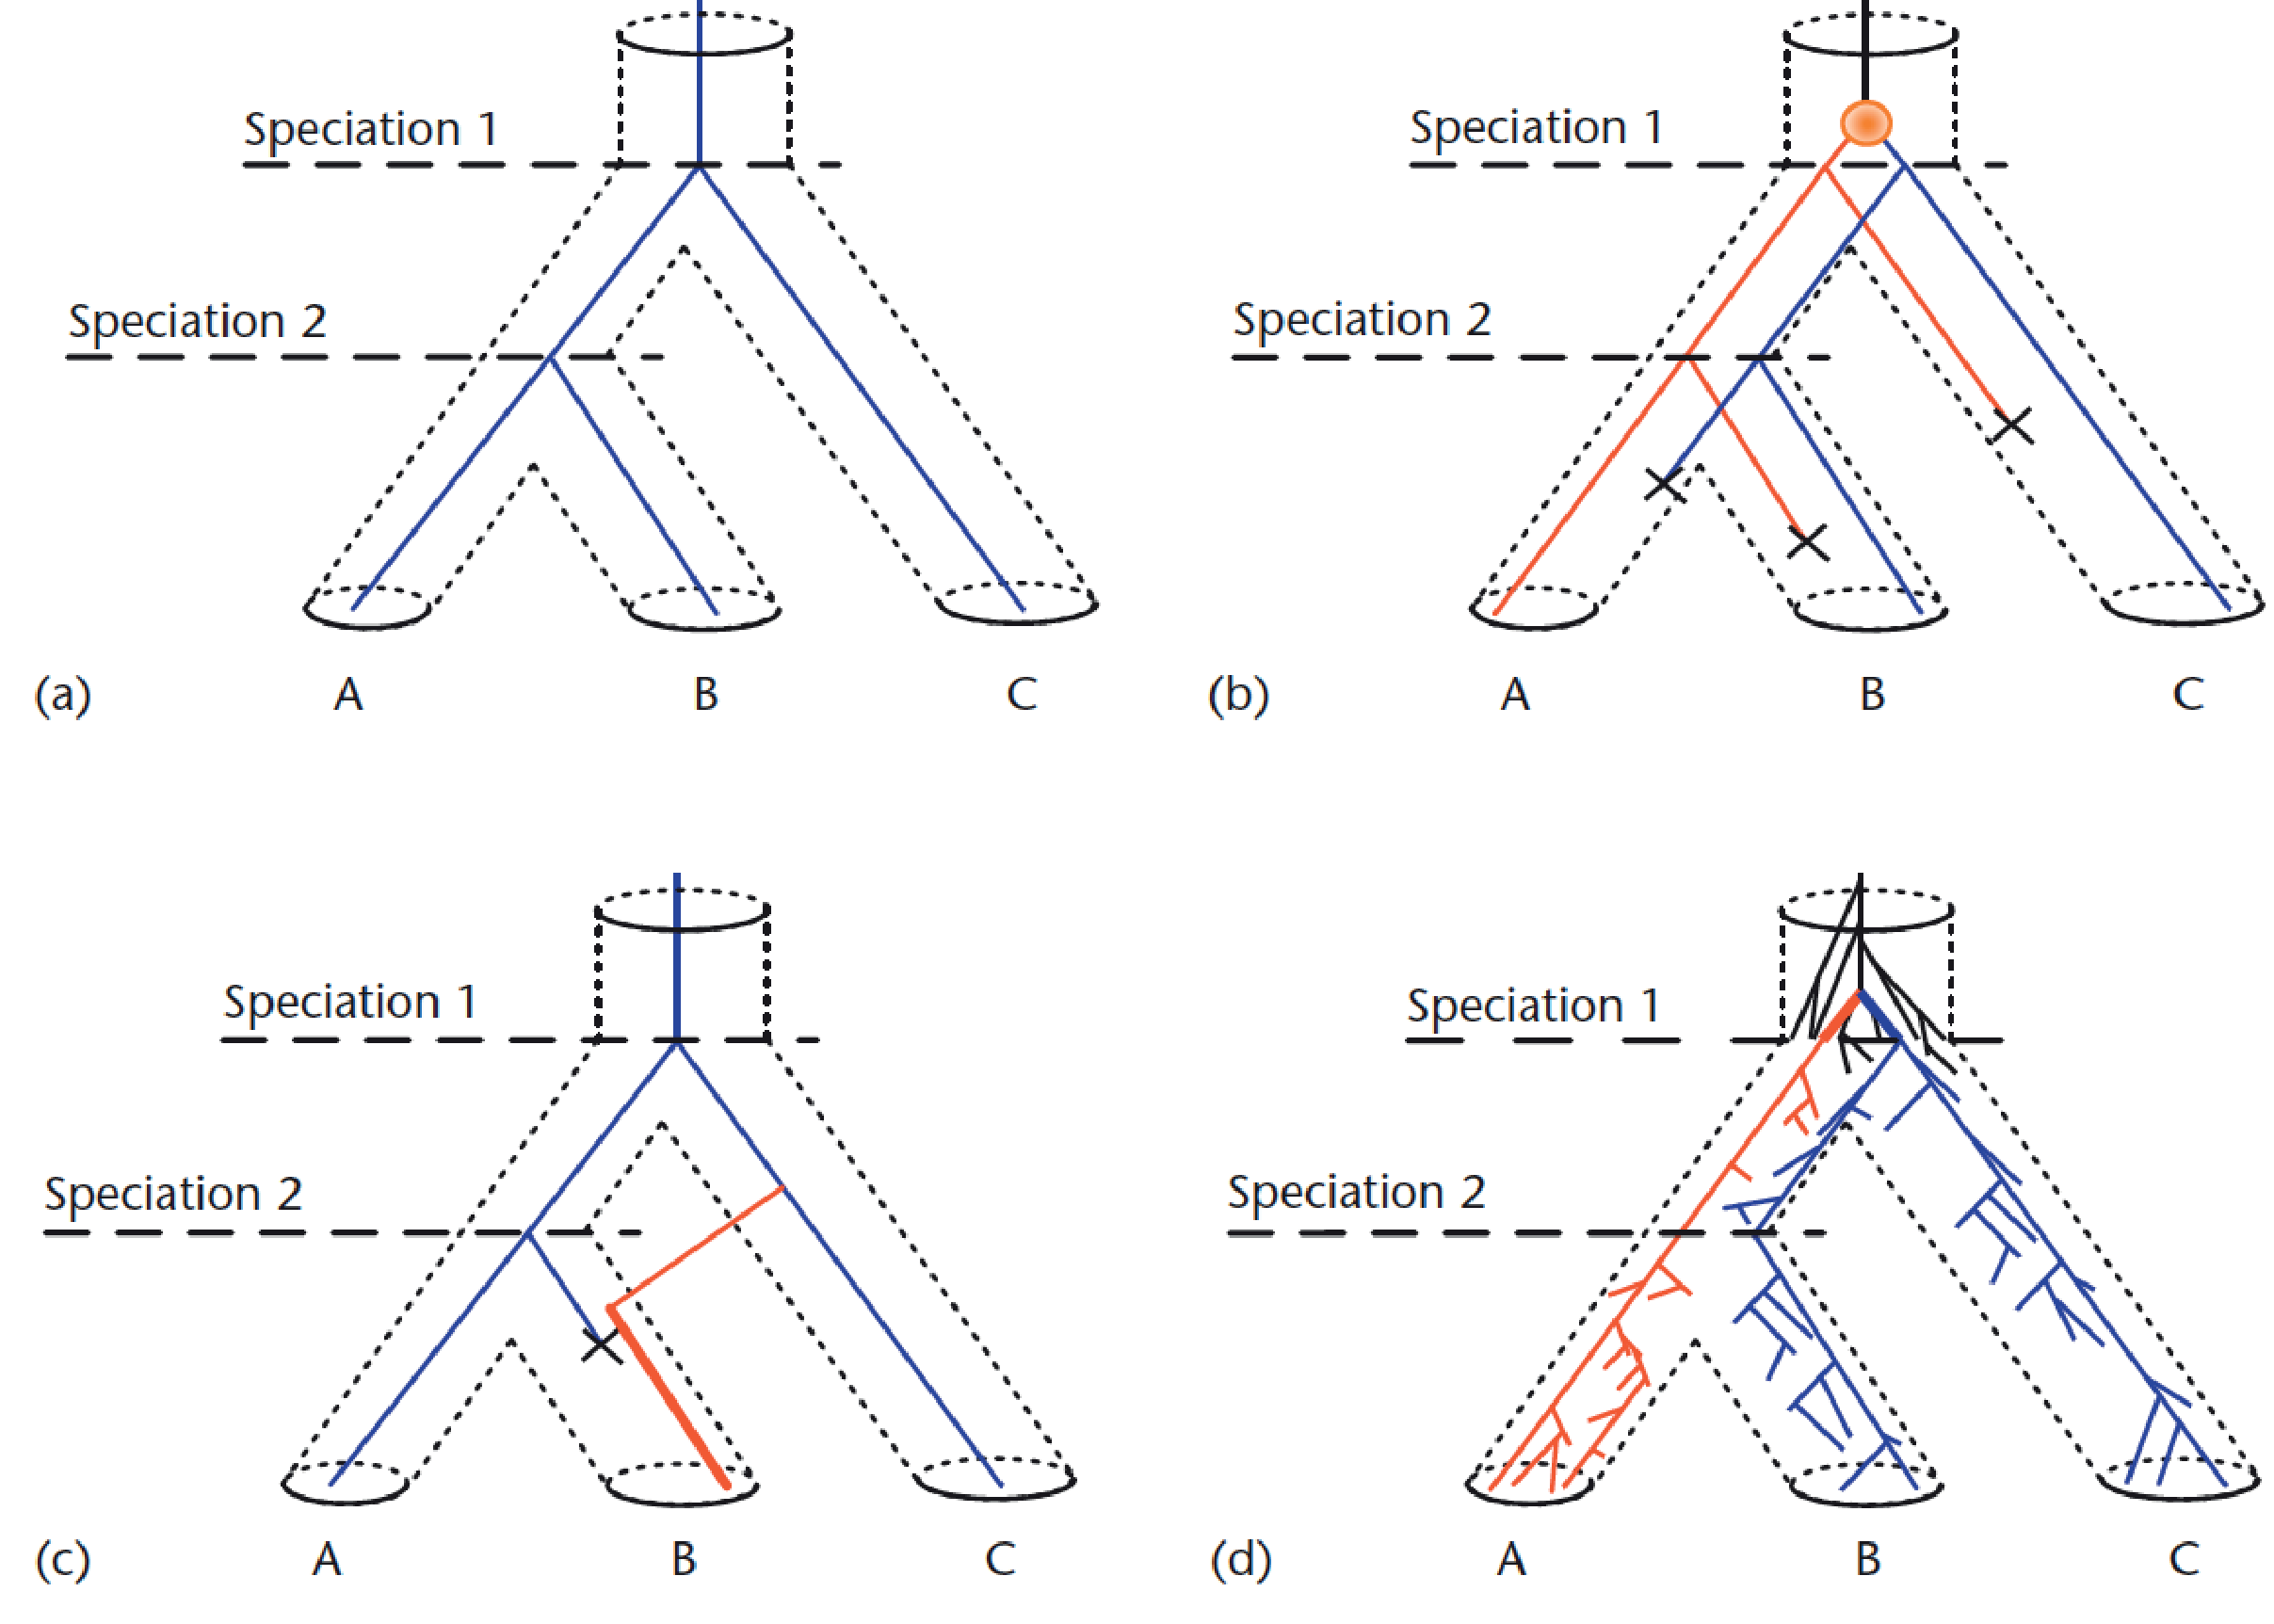
\includegraphics[width=5.8in,angle=0]{\ResourcePath figures/DupTransILS.pdf}}
\caption{\small The processes of discord. The species tree is represented as a tubular structure. Gene trees are blue and red lines running along the species trees. a) A gene tree that perfectly matches the species tree. b) The gene tree and the species tree differ because of gene duplications and losses. c)  The gene tree and the species tree differ because of gene transfer and gene loss. d)  The gene tree and the species tree differ because of incomplete lineage sorting.   [Replicated from Fig.~2 in \citet{Boussau2009}.]}
\label{fig1}
\end{figure}

Fig. \ref{fig1} suggests that for all processes the gene tree can be seen as the product of a branching process operating inside the species tree.
As a consequence, all processes are modeled as some type of birth-death process.
For duplication/loss models, birth correspond to gene duplication events, and death to gene loss events.
Transfers can be added to the model by introducing another type of birth, with a child lineage appearing in another branch of the species tree.
Incomplete lineage sorting is also modeled with a birth-death type of model, the coalescent.
All these models can be made heterogeneous, by allowing different sets of parameters for different branches of the species tree.
This is useful to model differences in rates of duplication, loss or transfer among species, or to model different effective population sizes in a species tree.
In \RevBayes~so far only models of incomplete lineage sorting have been implemented (models of duplication and loss and transfer will soon be added).
Thanks to \RevBayes~modular design, there is quite a lot of flexibility in specifying the model, for instance by allowing different parameters to different branches of the species tree, and the gene tree-species tree model could be combined to other types of models, for instance models of trait evolution.


\subsection{Gene tree discordance is a problem for species tree reconstruction}
There are several approaches to species tree reconstruction: concatenation and supertree approaches, which have been used for quite some time now, and more recently methods that rely on gene tree-species tree models.\begin{enumerate}
\item Concatenation simply consists in taking all gene alignments, concatenating them into one super alignment, and then analyzing it as if it were a single gene sequence.
Its main assumption is therefore that all sites of all genes have evolved according to the same species tree.
This assumption is not correct because all the processes of discord presented above conspire to make gene trees different from the species tree.
In practice, this matters: for instance, one can prove that in the presence of incomplete lineage sorting, in some particular area of the parameter space, concatenation will return an incorrect species tree.
Another example might be found in prokaryotic phylogenetics, where the quest for a tree of life has been very frustrating, to the point that many doubt that one could find a meaningful species tree representing vertical descent.
Recent models incorporating lateral gene transfer allow tackling this question in a more principled way.
\item Supertree approaches differ from concatenation notably by discarding sequence information once individual gene trees have been built.
They combine individual gene trees to obtain a species tree.
Most supertree methods are not based on an explicit model of the processes causing discordance between gene trees and species tree (although there are exceptions, notably modelling incomplete lineage sorting, see below).
Instead, they aim at finding a tree that would best describe the distribution of gene trees, according to some fairly arbitrary criterion.
In practice, these methods have been found to provide reasonable results in many cases, but in simulations are less accurate than concatenation.
\item Methods that rely on gene tree-species tree models appear very promising as they explicitly model the processes of discord, and can be combined with a model of sequence evolution, models of the co-evolution between gene trees, models of trait evolution... 
\end{enumerate}


\subsection{Modelling incomplete lineage sorting: the multispecies coalescent}
Incomplete lineage sorting is a population-level process.
In a species, at a given time, there are several alleles for a given locus in the genome.
These alleles have their own history, they diverged from each other at various times in the past.
This history can differ from the species history, because several alleles can persist through a speciation event, and because, short of selective effects, the sorting of alleles during a speciation event is random and can result in a tree that differs from the species tree (Fig. \ref{fig1}d).
In all cases, incongruence between the gene tree and the species tree occurs when alleles persist over the course of several speciation events.
When reconstructing a gene tree, one therefore gets the history of the alleles that have been sampled (at best), not necessarily the history of the species. 

In 2003, Rannala and Yang proposed a powerful way to model the sorting of alleles along a phylogeny of several species \citep{Rannala2003a}, the multispecies coalescent (Fig. \ref{fig2}).
This model is at the origin of most model-based approaches to reconstruct gene and species trees \citep{Edwards2007,Heled2010}.
The multispecies coalescent appropriately models the evolution of a population of alleles along a species tree.
Along the species tree, it allows different branch lengths, in units of time, and also allows different effective population sizes.
Computing the probability of a gene tree given a species tree and other parameters is quite easy.
Bascially it works by cutting the gene tree into independent species-specific subtrees, computing probabilities for each of those subtrees, and combining them all at the end to get the probability of the gene tree according to the multispecies coalescent, given the current parameter values.
Cutting the gene tree into species-specific subtrees is quite easy, because we can use the dates of speciation events to know what's before and after speciation events. 
The resulting subtrees are represented with the grey boxes in Fig. \ref{fig2}.
In this figure, each subtree corresponds to one particular population, either extant or ancestral.
Inside each subtree, given its length, the effective population size, and dates of coalescence (alleles splitting), the coalescent model provides simple formulas for computing the probability of the gene subtree given other parameters.
These subtree probabilities are then multiplied to get the gene tree probability given current parameter values.
 
Two parameters associated to branches of the species tree have a direct impact on the expected amount of gene tree-species tree incongruence:
\begin{itemize}
\item \textbf{Time between speciations.} The more a branch length increases, the more the pool of alleles is expected to change.
Alleles are therefore less likely to persist for several speciation events if the branches between these speciation events are long.
\item \textbf{Effective population size between speciations.} In populations with small effective population sizes, chance events can cause large shifts in allele frequencies, and possibly disappearance of alleles, irrespective of the fitness of this allele. 
In large populations, because an allele is likely carried by a large number of individuals, its disappearance is less likely, the population of alleles is more stable.
Alleles are therefore less likely to persist for several speciation events if the branches between these speciation events are characterised by small effective population sizes.
\end{itemize}
Overall, larger amounts of gene tree-species tree incongruence are expected in phylogenies characterised by short branches with large population sizes. 
A corollary of that is that larger amounts of gene tree-gene tree incongruence are expected as well. 
To measure the susceptibility of species phylogenies to generate incomplete lineage sorting, the concept of \emph{coalescent time units} has been introduced.
Coalescent time units are obtained when branch length $\lambda$ is divided by effective population size $N_e$.
As a consequence, in a species tree whose branches are expressed in coalescent time units, a branch length of $1~coalescent~time~unit $ means a branch length of $N_e~generations$. 
Once branch lengths on the species tree are measured in coalescent time units, it becomes easy to spot species trees that generate a lot of incongruence: those are short trees.

\begin{figure}[h!]
\centering
\fbox{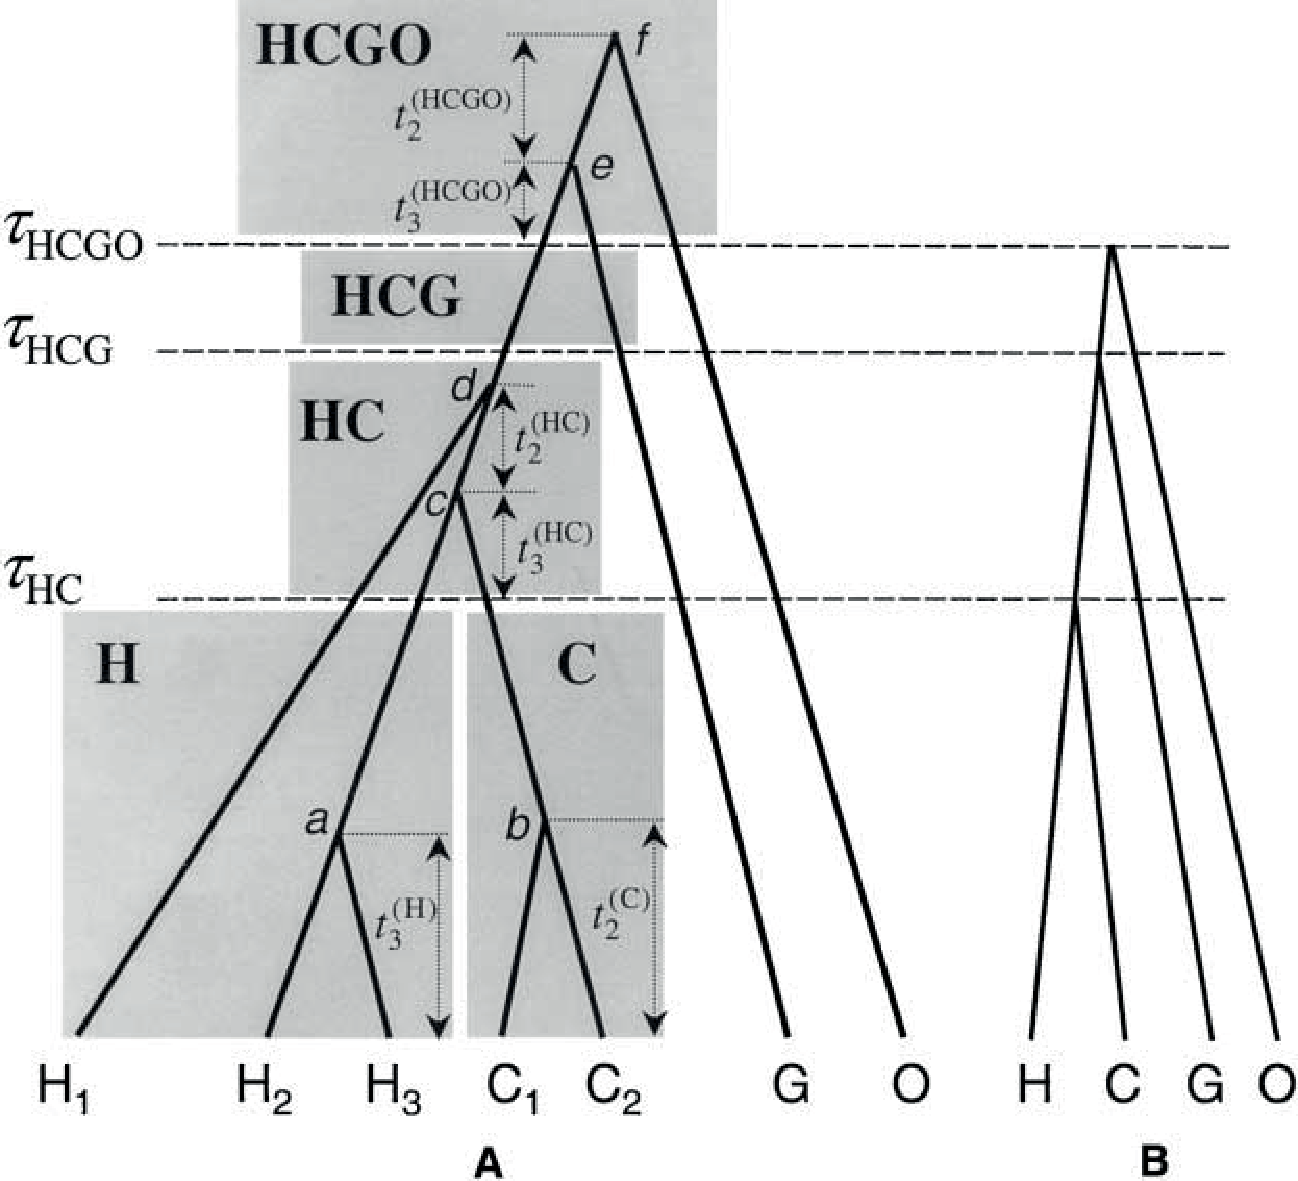
\includegraphics[width=5.8in,angle=0]{\ResourcePath figures/RannalaYang.pdf}}
\caption{\small The multispecies coalescent. A) A gene tree, including 3 human alleles, 2 Chimp alleles, one Gorilla allele, and one Orang-outan allele. $\tau$ parameters are speciation times, $t$ parameters are divergence time in the gene tree, the grey squares represent the ancestral populations, with their respeciive sizes.  B) The corresponding species tree. In this model, the speciation times define minimal boundaries for allele divergence times. [Replicated from Fig.~1 in \citet{Rannala2003a}.]}
\label{fig2}
\end{figure}

\vspace{20mm}

{\begin{framed}
\begin{center}
The exercises assume you have a working installation of RevBayes.
The first exercise aims at understanding the impact of the parameters of the multispecies coalescent.
The other exercises will introduce methods to reconstruct species trees and gene trees using the multispecies coalescent or closely-related models.
Scripts are all placed in {\footnotesize \emph{$tutorials/RB\_GeneTreeSpeciesTree\_Tutorial/RB\_GeneTreeSpeciesTree\_tutorial\_files/RevBayes\_scripts/$}}, in five folders. 
\emph{It is highly recommended to start RevBayes from each of these folders when doing the exercises.}
\end{center}
\end{framed}}
\vspace{5mm}

\begin{center}
\emph{First RevBayes exercise: simulating gene trees under the multispecies coalescent}
\end{center}
\begin{enumerate}
\item Open RevBayes
\item Let's simulate a species tree with 10 taxa, 10 gene trees, 5 alleles per species (feel free to change these values).
{\tt \begin{snugshade*}
\begin{lstlisting}
n_species <- 10
n_genes <- 10
n_alleles <- 5

# Species names
for (i in 1:n_species) {
	s_names[i] <- "Species_"+i
}
\end{lstlisting}
\end{snugshade*}}
\item We simulate a species tree topology according to a birth-death process with arbitrary parameter values (similar to \citet{Leache2011}):
{\tt \begin{snugshade*}
\begin{lstlisting}
speciation ~ dnExp(10.0)
extinction ~ dnExp(10.0)
tree_height ~ dnUniform(0,1.0)
speciation.setValue(2)
extinction.setValue(0.3)
tree_height.setValue(0.8)
speciesTree ~ dnBDP(lambda=speciation, mu=extinction, origin=tree_height, nTaxa=n_species, names=s_names)
\end{lstlisting}
\end{snugshade*}}
\item Then we can use the multispecies coalescent model to generate gene trees. These can be examined using Figtree or NJplot or any other tree viewer, but we can also directly compute symmetric differences between these from RevBayes. First, we simulate a set of gene trees, using a single effective population size for all branches, and after having constructed a map between species names and gene names:
{\tt \begin{snugshade*}
\begin{lstlisting}
# Build the mapping between sequence names and species names.
for (i in 1:n_species) {
	for (j in 1:n_alleles) {
		taxa[(i-1)*n_alleles+j] <- taxon(taxonName=s_names[i]+"_"+j, speciesName=s_names[i])
	}
}
# Set the effective population size
Ne ~ dnGamma(shape=0.1,rate=0.1)
Ne.setValue(0.004)
# Simulate gene trees
for (i in 1:n_genes) {
   # The gene tree from the multispecies coalescent process
   # Note that if Ne had been a vector of effective population sizes instead of a single value, 
   # allowing 1 parameter per branch of the species tree, the same line would work.
   geneTrees[i] ~ dnCoalMultiSpeciesConst(speciesTree=speciesTree, Ne=Ne, taxa=taxa)
}
\end{lstlisting}
\end{snugshade*}}

We write the data to file,  in the "dataFolder" directory.
{\tt \begin{snugshade*}
\begin{lstlisting}

# We need to save the species tree and the gene trees
write(speciesTree, filename=dataFolder+"speciesTree")

# Saving the gene trees
for (i in 1:(n_genes)) {
	write(geneTrees[i], filename=dataFolder+"geneTree_"+i+".tree")
}

\end{lstlisting}
\end{snugshade*}}


\item We can compute symmetric differences between all these gene trees. The symmetric difference between two trees is the total number of partitions found in one tree but not in the other one. In our case, the maximal difference is as follows:
{\tt \begin{snugshade*}
\begin{lstlisting}
maxDiff <- 2 * (n_species*n_alleles - 2)
\end{lstlisting}
\end{snugshade*}}
\item That will give us a reference for comparing with the values we get on our gene trees. We can build a function for computing all pairwise symmetric differences between our gene trees, and getting the mean. Caveat: in the current state of the Rev language, we have to use variable names that have never been used before in the workspace (hence the use of "k" and "l" for loop indices instead of "i" and "j" that have been used before. Alternatively we could have done a "clear(i)" and a "clear(j)" if we really wanted to use these variable names). 

{\tt \begin{snugshade*}
\begin{lstlisting}
function RealPos symDiffVector ( TimeTree[] vec ) {
	ndiff <- 1
	for (k in 1:(vec.size()-1)) {
		for (l in (k+1):vec.size()) {
			diff[ndiff]<-symDiff (vec[k], vec[l])
			ndiff <- ndiff+1
		}
	}
	return (mean(diff))
}


#We can then use this function on our gene trees:
symDiffVector(geneTrees)
\end{lstlisting}
\end{snugshade*}}
\item Now to get a sense of how population size and branch lengths alter the gene tree distribution, we can relaunch the multispecies coalescent simulation (step 4) and look at the resulting gene trees after having rescaled the species tree or changed the effective population size. To do these little changes: 
 {\tt \begin{snugshade*}
\begin{lstlisting}
# Changing Ne: 
Ne.setValue(0.08)
#Rescaling the species tree:
speciesTree.rescale(0.1)
\end{lstlisting}
\end{snugshade*}}
\end{enumerate}
\emph{Using the functions above, it is possible to look at the species tree in coalescent time units (which is very convenient). How would you do that?}

\emph{Do these observations seem coherent with the multispecies coalescent presentation above?}



\bigskip
\section{Alternatives to the multispecies coalescent model}
\subsection{Strengths and weaknesses of the multispecies coalescent}

The multispecies coalescent model is an elegant model. 
As we have seen above, we can easily simulate data under this model.
Inference using this model, combined with a model of sequence evolution, is also possible, and when it works, is very informative.
Not only can we get a dated species tree and dated gene trees from the multispecies coalescent, we can also get extant and ancestral effective population sizes \citep{Edwards2007,Heled2010}.
However inferring many parameters is difficult, and convergence can be difficult to reach with such models.
In particular, the strong interdependence that exists between the gene trees and the species tree makes it easy for algorithms to fall into local maxima.
As a consequence, there are ongoing efforts to develop methods for which inference would be easier, albeit at the cost of approximations and simplifications.

\subsection{Alternatives to the multispecies coalescent}
An easy way to simplify the problem is to consider that parts of it are already solved.
For instance, several approaches assume that rooted gene trees are available.
The problem then becomes markedly easier, but inference is then highly dependent on the quality of the input gene trees. 
Often, such methods also make other simplifying assumptions, and e.g. do not try to estimate separately time and effective population sizes, but instead directly work with coalescent time units.
These methods usually are much faster than the multispecies coalescent, should be more robust against local maxima, but are less ambitious about the amount of information they can get from the data, and are can be sensitive to the quality of the input gene trees.

Another approach is to use methods that mathematically bypass estimating gene trees altogether.
To our knowledge, there are three such approaches: SNAPP \citep{Bryant2012}, POMO \citep{DeMaio2013}, and SVDQuartets \citep{Chifman2014}.
They differ in the way the algorithms work, but they are all based on the same idea, which is integrating out gene trees.
To achieve that they extend the model of sequence evolution, which usually models substitution events, to also model population-level processes.
In RevBayes, so far only the POMO model has been implemented and will be discussed in the following part.

\subsection{The POMO model}
POMO models allele frequency changes along with mutations with a single transition matrix.
It extends the usual $4\times4$ DNA substitution matrix to incorporate polymorphic states.
In doing so, it makes a first important approximation: it only considers biallelic states.
For instance, it considers sites at which either an A or a C is found in a population, but it won't consider sites at which 3 different states, e.g. A, C, T, are observed in a population.
Then it makes a second approximation, which introduces a single virtual population size in lieu of the branchwise effective population sizes.
This virtual population size is not inferred, but is fixed to some low number.
In practice, \citet{DeMaio2013} consider that a virtual population size of 10 individuals should produce good results.
This virtual population size directly constrains the types of polymorphic states that can be considered.
With 10 individuals for instance, only frequencies such as $(100\%A)$, $(10\%A, 90\%C)$, $(20\%A, 80\%C)$, $(30\%A, 70\%C)$, ..., $(90\%A, 10\%C)$, $(100\%C)$ can be considered.
The POMO matrix models transitions among all these states, polymorphic ones as well as monomorphic ones, and has a size that depends on the virtual population size.
For instance, with a virtual population size of 10 individuals, the POMO square matrix contains $58$ rows: 4 monomorphic states, plus 6 types of biallelic states ($AC, AG, AT, CG, CT, GT$) times 9 frequencies.
Additional assumptions of the POMO model include total independence among sites (no linkage among sites), and absence of mutations in biallelic states: transitions among biallelic states or from biallelic states to monoallelic states only occur through population-level changes in allele frequencies, not through mutation of one allele into another.
Mutations only occur to transit from a monoallelic state to a biallelic state.

The POMO model therefore makes several approximations to avoid estimating gene trees.
Fewer parameters need to be estimated, as neither gene trees nor population sizes are estimated, but other parameters can be introduced into the model.
For instance \citet{DeMaio2013} estimate 4 base fitness parameters, which they use to model GC-biased gene conversion, which tends to increase the GC content of recombining sequences.
In the RevBayes implementation of POMO, base fitnesses can be estimated as well.

\bigskip
\section{Inference using the multispecies coalescent, the POMO model, and basic concatenation}
In this section we will perform inference using the multispecies coalescent, the POMO model, and concatenation.
Depending on your machine and on the size of the data, successful inference may take some time.
If this tutorial is done in a classroom environment, it may be wise to convene with friends that one tries the multispecies coalescent model while another one tries the POMO model, and the third one tries the concatenation approach, and that results will be shared.
In case you want to compare the results between machines or between RevBayes sessions, you have to make sure that you are using the same random seed in all sessions. This is easily done by setting the seed using 
 {\tt \begin{snugshade*}
\begin{lstlisting}
seed(x, y)
\end{lstlisting}
\end{snugshade*}}
where $x$ and $y$ are two integer numbers of your choice.

First we will simulate data, and then we will perform inference using the three different approaches.

%%%%%%%%%%%%%%%%%%%%%%%%%%%%%%%%%%%%%%%%%%%
%%%%%%%%%%%%%%%%%%%%%%%%%%%%%%%%%%%%%%%%%%%
%%%%%%%%%%%%%%%%%%%%%%%%%%%%%%%%%%%%%%%%%%%
\subsection{Simulating data}
We are going to do inference on simulated data, as produced during the previous section.
However in addition to the species tree and the gene trees, we will be producing sequence data.
Below is the RevBayes code necessary to simulate all the data.
As before, parameters of the simulation can be changed as seems fit, but here we chose parameters that resemble \citet{Leache2011}.

{\begin{framed}
\begin{center}
\emph{WARNING: The following script may be less up to date than the simulation scripts named "UnderstandingMultiSpeciesCoalescent/MultiSpeciesCoalescentSimulatingTreesAndAlignments.Rev".}
\end{center}
\end{framed}}
\vspace{5mm}


{\begin{framed}
First we can set the folder in which we will save the output of our work.
 {\tt \begin{snugshade*}
\begin{lstlisting}
dataFolder<-"/PATH/TO/A/FOLDER/WHERE/TO/SAVE/THE/OUTPUT"
setwd(dataFolder)
\end{lstlisting}
\end{snugshade*}}

Let's simulate a species tree with 6 taxa, 10 gene trees, 5 alleles per species, and along each gene tree one gene alignment 200 bases long.
It's a small data set, designed for manageable inference during a tutorial, but patient users may want to simulate a larger data set.

 {\tt \begin{snugshade*}
\begin{lstlisting}
n_species <- 10
n_genes <- 10
n_alleles <- 5
n_sites <- 100
n_branches <- 2 * n_species - 3 # number of branches in a rooted tree
\end{lstlisting}
\end{snugshade*}}

The species-tree birth-death model:

{\tt \begin{snugshade*}
\begin{lstlisting}
# Species names
for (i in 1:n_species) {
   s_names[i] <- "Species_"+i
}
speciation ~ dnExp(10.0)
extinction ~ dnExp(10.0)
tree_height ~ dnUniform(0,1.0)
speciation.setValue(2)
extinction.setValue(0.3)
tree_height.setValue(0.008)
# Species tree from birth-death process
speciesTree ~ dnBDP(lambda=speciation, mu=extinction, origin=tree_height, nTaxa=n_species, names=s_names)
# Making a backup for future reference:
trueSpeciesTree <- speciesTree
\end{lstlisting}
\end{snugshade*}}

The gene-tree multispecies coalescent model
 {\tt \begin{snugshade*}
\begin{lstlisting}
# Build the mapping between sequence names and species names.
for (i in 1:n_species) {
   for (j in 1:n_alleles) {
       taxa[(i-1)*n_alleles+j] <- taxon(taxonName=s_names[i]+"_"+j, speciesName=s_names[i])
   }
}
# Set the effective population size
Ne ~ dnGamma(shape=0.5,rate=0.5)
Ne.setValue(0.004)
# Simulate gene trees
for (i in 1:n_genes) {
   # The gene tree from the multispecies coalescent process
   # Note that if Ne had been a vector of effective population sizes, 
   # allowing 1 parameter per branch of the species tree, the same line would work.
   geneTrees[i] ~ dnCoalMultiSpeciesConst(speciesTree=speciesTree, Ne=Ne, taxa=taxa)
}
# Making a backup for future reference:
trueGeneTrees <- geneTrees
trueNe <- Ne
\end{lstlisting}
\end{snugshade*}}

Substitution models will all be based on the GTR model. However, the parameters of the models change from one gene family to the next.
 {\tt \begin{snugshade*}
\begin{lstlisting}
for (i in 1:n_genes) {
  er_prior[i] <- v(1,1,1,1,1,1)
  er[i] ~ dnDirichlet(er_prior[i])
  sf_prior[i] <- v(1,1,1,1)
  sf[i] ~ dnDirichlet(sf_prior[i])
  Q[i] := fnGTR(er[i],sf[i]) 
}
# Making a backup for future reference:
for (i in 1:n_genes) {
	trueEr[i] <- er[i]
	trueSf[i] <- sf[i]
}
\end{lstlisting}
\end{snugshade*}}

Then we assume a strict clock Model, but of course we could assume a relaxed clock.
Each gene family can have its own rate of evolution, drawn from an exponential distribution.
 {\tt \begin{snugshade*}
\begin{lstlisting}
for (i in 1:n_genes) {
  familyRates[i] ~ dnExp(1.0)
}
# Making a backup for future reference:
for (i in 1:n_genes) {
  trueFamilyRates[i] <- familyRates[i] 
}
\end{lstlisting}
\end{snugshade*}}

We add a model of among-site rate variation, handled by a discretized Gamma distribution, one for each gene family:

 {\tt \begin{snugshade*}
\begin{lstlisting}
for (i in 1:n_genes) {
  shape_prior[i] <- 0.05 
  shape[i] ~ dnExponential( shape_prior[i] )
  norm_gamma_rates[i] := fnDiscretizeGamma( shape[i], shape[i], 4, false )
}
\end{lstlisting}
\end{snugshade*}}

Finally we link it all using the PhyloCTMC model, which simulates gene alignments:

 {\tt \begin{snugshade*}
\begin{lstlisting}
for (i in 1:n_genes) {
  alns[i] ~ dnPhyloCTMC(tree=geneTrees[i], Q=Q[i],  branchRates=familyRates[i], siteRates=norm_gamma_rates[i], nSites=n_sites, type="DNA")
}
\end{lstlisting}
\end{snugshade*}}
We can then save the simulated data to the folder chosen at the beginning of this script.
We need to save the species tree, the gene trees, and the gene alignments

 {\tt \begin{snugshade*}
\begin{lstlisting}
write(speciesTree, filename="speciesTree")
for (i in 1:n_genes) {
	write(geneTrees[i], filename="geneTree_"+i)
}
for (i in 1:n_genes) {
	writeFasta(alns[i], filename="alignment_"+i+".fasta")
}
\end{lstlisting}
\end{snugshade*}}
\end{framed}}

%%%%%%%%%%%%%%%%%%%%%%%%%%%%%%%%%%%%%%%%%%%
%%%%%%%%%%%%%%%%%%%%%%%%%%%%%%%%%%%%%%%%%%%
%%%%%%%%%%%%%%%%%%%%%%%%%%%%%%%%%%%%%%%%%%%
\subsection{Inference using the multispecies coalescent }
{\begin{framed}
\begin{center}
\emph{WARNING: The following script may be less up to date than the simulation script named "MultiSpeciesCoalescentWithSequences/MultiSpeciesCoalescentWithSequencesMCMC.Rev".}
In the following we perform inference from the alignments, but we could also do inference directly from the gene trees, as can be seen in the script "MultiSpeciesCoalescent/MultiSpeciesCoalescentMCMC.Rev".
\end{center}
\end{framed}}
\vspace{5mm}


Now that we have simulated data, we can run inference under the multispecies coalescent, using the sequences as input data.

{\begin{framed}
First we clamp the alignments:
{\tt \begin{snugshade*}
\begin{lstlisting}
for (i in 1:n_genes) {
	alns[i].clamp(alns[i])
}
\end{lstlisting}
\end{snugshade*}}

Then we change the starting values, because we want to start from random values, not the values used in the simulation.

{\tt \begin{snugshade*}
\begin{lstlisting}
# Redrawing the parameters of the birth-death process:
speciation.redraw()
extinction.redraw()
tree_height.redraw()
# Redrawing the species tree:
speciesTree.redraw()
# Redrawing the parameter Ne:
Ne.redraw()
# Redrawing the gene trees:
for (i in 1:n_genes) {
   geneTrees[i].redraw()
}
# Redrawing the parameters of the substitution models:
for (i in 1:n_genes) {
  er[i].redraw()
  sf[i].redraw()
}
# Idem for the family-wise rates of sequence evolution:
for (i in 1:n_genes) {
  familyRates[i].redraw()
}
# Idem for the family-wise across-site rate variation parameters:
for (i in 1:n_genes) {
  shape[i].redraw()
}
\end{lstlisting}
\end{snugshade*}}

We need to set up moves for the birth-death parameters, the species tree topology, the gene tree topologies, the parameter Ne, the parameters of the substitution models, the rates on the gene trees.

{\tt \begin{snugshade*}
\begin{lstlisting}
moveIndex <- 0
# moves for the birth-death parameters
moves[moveIndex++] <- mvScale(speciation,1,true,1.0) # In the revLanguage, table indices start at 1
moves[moveIndex++] <- mvScale(extinction,1,true,1.0)
moves[moveIndex++] <- mvSlide(tree_height,delta=1.0,true,2.0)
# moves on the tree topology and node ages
moves[moveIndex++] <- mvNNI(speciesTree, 1.0)
moves[moveIndex++] <- mvFNPR(speciesTree, 1.0)
moves[moveIndex++] <- mvSubtreeScale(speciesTree, 5.0)
moves[moveIndex++] <- mvTreeScale(speciesTree, delta=1.0, tune=true, weight=3.0)
moves[moveIndex++] <- mvNodeTimeSlideUniform(speciesTree, 10.0)
moves[moveIndex++] <- mvRootTimeSlide(speciesTree, 1.0, true, 3.0)
# moves on the gene tree topologies and node ages
for (i in 1:n_genes) {
   moves[moveIndex++] <- mvNNI(geneTrees[i], 1.0)
   moves[moveIndex++] <- mvFNPR(geneTrees[i], 1.0)
   moves[moveIndex++] <- mvSubtreeScale(geneTrees[i], 5.0)
   moves[moveIndex++] <- mvTreeScale(geneTrees[i], delta=1.0, tune=true, weight=3.0)
   moves[moveIndex++] <- mvNodeTimeSlideUniform(geneTrees[i], 10.0)
   moves[moveIndex++] <- mvRootTimeSlide(geneTrees[i], 1.0, true, 3.0)
}
# move on Ne, the effective population size
moves[moveIndex++] <- mvScale(Ne,1,true,1.0)
# moves on the parameters of the substitution models
for (i in 1:n_genes) {
  moves[moveIndex++] <- mvSimplexElementScale(er[i], alpha=10, tune=true, weight=3) 
  moves[moveIndex++] <- mvSimplexElementScale(sf[i], alpha=10, tune=true, weight=2) 
}
# moves on the family-wise rates
for (i in 1:n_genes) {
  moves[moveIndex++] <- mvScale(familyRates[i], lambda=0.8, tune=true, weight=3.0)
}
# moves on the across-sites rate variation parameters:
for (i in 1:n_genes) {
  moves[moveIndex++] <- mvScale(shape[i], lambda=0.8, tune=true, weight=3.0)
}
\end{lstlisting}
\end{snugshade*}}

Then we define a few monitors to keep track of how things go. 
First, basic monitors:
{\tt \begin{snugshade*}
\begin{lstlisting}
mntrIndex <- 0
# One monitor to backup the parameters, in case we want to stop and restart the analysis:
monitors[mntrIndex++] <- mnModel(filename="multispeciesCoalescent_clock.log",printgen=10, separator = "	")
# One monitor to print the species trees sampled in the course of the MCMC:
monitors[mntrIndex++] <- mnFile(filename="multispeciesCoalescent_clock_species.trees",printgen=10, separator = "	", speciesTree)
# One monitor for each gene family tree:
for (i in 1:n_genes) {
   monitors[mntrIndex++] <- mnFile(filename="multispeciesCoalescent_clock_gene_"+ i +".trees",printgen=10, separator = "	", geneTrees[i])
}
\end{lstlisting}
\end{snugshade*}}
We will also compare our reconstructed parameters (trees or other variables) to the true values that were used in the simulation.
First, examining the species tree and the gene trees.
{\tt \begin{snugshade*}
\begin{lstlisting}
distSpeciesTree := symDiff (trueSpeciesTree, speciesTree)
for (i in 1:n_genes) {
	distGeneTree[i] := symDiff (trueGeneTrees[i], geneTrees[i])
}
# We get one average value for all gene trees:
meanDistGeneTree := mean(distGeneTree)
\end{lstlisting}
\end{snugshade*}}

We can also look at the values of some other variables:
{\tt \begin{snugshade*}
\begin{lstlisting}
# For Ne:
distNe := Ne - trueNe
# For equilibrium values of the GTR matrices, we want one index of how far we are.
# To achieve this we need to write some functions:
clear(i)
distEqFreq := diffVectorsOfVectors(trueSf, sf)	
function RealPos diffVectors ( Real[] xvec, Real[] yvec ) { 
	DI <- 0.0
	for (i in 1:xvec.size()) {
		DI <- DI + (xvec[i] - yvec[i])*(xvec[i] - yvec[i])
	}
	return DI
}
function RealPos diffVectorsOfVectors ( Real[][] xvecvec, Real[][] yvecvec ) { 
	DA <- 0.0
	for (i in 1:xvecvec.size()) {
		DA <- DA + diffVectors(xvecvec[i], yvecvec[i])
	}
	return DA
}		
function RealPos diffVectorsOfVectors ( Simplex[] xvecvec, Simplex[] yvecvec ) { 
	DA <- 0.0
	for (i in 1:xvecvec.size()) {
		DA <- DA + diffVectors(xvecvec[i], yvecvec[i])
	}
	return xvecvec[2]
}
# Same thing for exchangeability parameters:
distExchange := diffVectorsOfVectors(trueEr, er)
monitors[mntrIndex++] <- mnScreen(printgen=10, distExchange)
# Same thing for the family-wise rates
distRates := diffVectors(trueFamilyRates, familyRates)
monitors[mntrIndex++] <- mnScreen(printgen=10, distRates)
# We can use one monitor that will output on the screen one parameter, Ne, distNe, distSpeciesTree, meanDistGeneTree, and distEqFreq:
monitors[mntrIndex++] <- mnScreen(printgen=10, Ne, distNe, distSpeciesTree, meanDistGeneTree, distEqFreq)
# We could do similar things for the few remaining parameters, but really I think that's enough.
\end{lstlisting}
\end{snugshade*}}

We then define our model and the mcmc object. We can use any node of our model as a handle, here we choose to use the species tree.
{\tt \begin{snugshade*}
\begin{lstlisting}
mymodel <- model(speciesTree)
# We create the MCMC object
mymcmc <- mcmc(mymodel, monitors, moves)
\end{lstlisting}
\end{snugshade*}}

We finally launch the analysis.
{\tt \begin{snugshade*}
\begin{lstlisting}
# If we want to specify the amount of burnin:
# mymcmc.burnin(generations=200,tuningInterval=100)
mymcmc.run(generations=400)

\end{lstlisting}
\end{snugshade*}}


After the analysis, we analyze the output. We analyze the tree trace as saved in one of the output files.
{\tt \begin{snugshade*}
\begin{lstlisting}
# Let us start by reading in the tree trace
 treetrace <- readTreeTrace("multispeciesCoalescent_clock_species.trees")
# and get the summary of the tree trace
 treetrace.summarize()

# We output the Maximum A Posteriori tree
 mapTree(treetrace,"primates_clock_MAP.tre")

\end{lstlisting}
\end{snugshade*}}

Of course, we could do the same analysis with each of the gene trees, possibly using a "for" loop in the rev language.

\end{framed}}

%%%%%%%%%%%%%%%%%%%%%%%%%%%%%%%%%%%%%%%%%%%
%%%%%%%%%%%%%%%%%%%%%%%%%%%%%%%%%%%%%%%%%%%
%%%%%%%%%%%%%%%%%%%%%%%%%%%%%%%%%%%%%%%%%%%
\subsection{Inference using the POMO model }

{\begin{framed}
\begin{center}
\emph{WARNING: The following script may be less up to date than the simulation script named "MultiSpeciesCoalescentAndPomo/MultiSpeciesCoalescentPomoMCMC.Rev".}
\end{center}
\end{framed}}
\vspace{5mm}


We run the POMO model on the same data set simulated under the multispecies coalescent.
 {\begin{framed}
 First, we need to prepare the data for analysis using POMO: concatenating the alignments, then transforming the state space from 4 bases to the POMO state space.
 We arbitrarily decide to use a virtual population size of size 10, as suggested in \citet{DeMaio2013}.
 {\tt \begin{snugshade*}
\begin{lstlisting}
# First, concatenating the alignments:
concatenate<-alns[1]
for (i in 2:n_genes) {
	concatenate <- concatenate + alns[i]
}

virtual_population_size <- 10

# Now, we need to convert the DNA alignment into an alignment in the correct POMO state space.

pomo_concatenate <- pomoStateConvert(concatenate, virtual_population_size, taxa)
concatenate_n_sites <- pomo_concatenate.nchar()[1]
\end{lstlisting}
\end{snugshade*}}
Now we have the data for doing inference using the POMO model.
To define a POMO model, one needs several components.
First, one needs to define a transition matrix for DNA mutations.
Here we are going to use a GTR matrix. 

 {\tt \begin{snugshade*}
\begin{lstlisting}


er_prior <- v(1,1,1,1,1,1)
er ~ dnDirichlet(er_prior)

sf_prior <- v(1,1,1,1)
sf ~ dnDirichlet(sf_prior)

Q := fnGTR(er,sf) 
\end{lstlisting}
\end{snugshade*}}

Second, one can have different fitnesses for A, C, G, T. 
Here, we are going to assume that all 4 bases have the same fitness.

 {\tt \begin{snugshade*}
\begin{lstlisting}
base_fitnesses <- v(1, 1, 1, 1)
\end{lstlisting}
\end{snugshade*}}
Now we have all the elements to build a POMO matrix to model the evolution of a population of alleles along a species tree.
 {\tt \begin{snugshade*}
\begin{lstlisting}
P := fnPomo(Q, base_fitnesses, virtual_population_size)
\end{lstlisting}
\end{snugshade*}}

We also need to define root frequencies for all the states.
To do that we need two variables:

 {\tt \begin{snugshade*}
\begin{lstlisting}
# First, the proportion of polymorphic sites at the root
root_polymorphism_proportion ~ dnBeta(alpha=1,beta=1)

# Second, one needs the root frequencies (we could use those of the GTR matrix but choose to have a non-stationary model):
root_base_frequencies ~ dnDirichlet(sf_prior)
\end{lstlisting}
\end{snugshade*}}

Now we have all the elements to construct root frequencies for all the states:
 {\tt \begin{snugshade*}
\begin{lstlisting}

root_frequencies := pomoRF (root_base_frequencies, root_polymorphism_proportion, Q, virtual_population_size)
#simplex_root_frequencies := simplex(root_frequencies[1], root_frequencies[2], root_frequencies[3], root_frequencies[4])

\end{lstlisting}
\end{snugshade*}}

Adding an across site rate variation model, the usual Gamma distribution discretized in 4 categories:
 {\tt \begin{snugshade*}
\begin{lstlisting}

shape_prior <- 0.05 
shape ~ dnExponential( shape_prior )
norm_gamma_rates := fnDiscretizeGamma( shape, shape, 4, false )

# We do not assume variation among branches in rates
branch_rates <- 1.0

# We do not assume a proportion of invariant
p_inv ~ dnBeta(alpha=1,beta=1)
p_inv.setValue(0.000001)
\end{lstlisting}
\end{snugshade*}}

Combining it all with the PhyloCTMC Model and clamp the model to the data:
 {\tt \begin{snugshade*}
\begin{lstlisting}

aln ~ dnPhyloCTMC(tree=speciesTree, Q=P, rootFreq=root_frequencies, branchRates=branch_rates, siteRates=norm_gamma_rates, pInv=p_inv, nSites=concatenate_n_sites, type="Standard")

aln.clamp(pomo_concatenate)
\end{lstlisting}
\end{snugshade*}}

Changing the starting values, we want to start from random values, not the values used in the simulation:

 {\tt \begin{snugshade*}
\begin{lstlisting}

# Redrawing the parameters of the birth-death process:
speciation.redraw()
extinction.redraw()
tree_height.redraw()

# Redrawing the species tree:
speciesTree.redraw()


\end{lstlisting}
\end{snugshade*}}


Then we need to set up moves for the birth-death parameters, the species tree topology, the gene tree topologies, the parameter Ne, the parameters of the substitution models, the rates on the gene trees.
 {\tt \begin{snugshade*}
\begin{lstlisting}

moveIndex <- 0

# moves for the birth-death parameters
moves[moveIndex++] <- mvScale(speciation,1,true,1.0) # In the revLanguage, table indices start at 1
moves[moveIndex++] <- mvScale(extinction,1,true,1.0)
moves[moveIndex++] <- mvSlide(tree_height,delta=1.0,true,2.0)


# moves on the tree topology and node ages
moves[moveIndex++] <- mvNNI(speciesTree, 1.0)
moves[moveIndex++] <- mvFNPR(speciesTree, 1.0)
moves[moveIndex++] <- mvSubtreeScale(speciesTree, 5.0)
moves[moveIndex++] <- mvTreeScale(speciesTree, delta=1.0, tune=true, weight=3.0)
moves[moveIndex++] <- mvNodeTimeSlideUniform(speciesTree, 10.0)
moves[moveIndex++] <- mvRootTimeSlide(speciesTree, 1.0, true, 3.0)

# moves on the parameters of the substitution model
moves[moveIndex++] <- mvSimplexElementScale(er, alpha=10, tune=true, weight=3) 
moves[moveIndex++] <- mvSimplexElementScale(sf, alpha=10, tune=true, weight=2) 

# moves on the 4 fitness values
# SH: These are not stochastic nodes, so moves cannot operate on them!
#moves[moveIndex++] <- mvScale(base_fitnesses[1],1,true,1.0)
#moves[moveIndex++] <- mvScale(base_fitnesses[2],1,true,1.0)
#moves[moveIndex++] <- mvScale(base_fitnesses[3],1,true,1.0)
#moves[moveIndex++] <- mvScale(base_fitnesses[4],1,true,1.0)

# moves on the parameters of the root frequencies
moves[moveIndex++] <- mvSimplexElementScale(root_base_frequencies, alpha=10, tune=true, weight=3) 
#moves[moveIndex++] <- mvScale(root_polymorphism_proportion, lambda=10, tune=true, weight=2) 
moves[moveIndex++] <- mvSlide(root_polymorphism_proportion, delta=10, tune=true, weight=2) 

# moves on the across-sites rate variation parameter:
moves[moveIndex++] <- mvScale(shape, lambda=0.8, tune=true, weight=3.0)
\end{lstlisting}
\end{snugshade*}}

Then we define a few monitors to keep track of how things go:
 {\tt \begin{snugshade*}
\begin{lstlisting}
mntrIndex <- 0

# One monitor to backup the parameters, in case we want to stop and restart the analysis:
monitors[mntrIndex++] <- mnModel(filename="pomo_clock.log",printgen=10, separator = "	")

# One monitor to print the species trees sampled in the course of the MCMC:
monitors[mntrIndex++] <- mnFile(filename="pomo_clock_species.trees",printgen=10, separator = "	", speciesTree)

# We also want to monitor how far we are from the true values, which we have because we rely on simulations.
# First, we can compute the distance between the reconstructed and the true species tree:
distSpeciesTree := symDiff (trueSpeciesTree, speciesTree)


# We can use one monitor that will output on the screen one parameter, Ne, distNe, distSpeciesTree, meanDistGeneTree, and distEqFreq:
monitors[mntrIndex++] <- mnScreen(printgen=10, distSpeciesTree)
\end{lstlisting}
\end{snugshade*}}
We define our model:
 {\tt \begin{snugshade*}
\begin{lstlisting}
# First we need to get rid of several variables that are not part of the Pomo model.
clear(alns)
clear(geneTrees)
clear(Ne)
clear(familyRates)
clear(trueEr)
clear(trueFamilyRates)
clear(trueGeneTrees)
clear(trueNe)
clear(trueSf)

# We can use any node of our model as a handle, here we choose to use the species tree.
 
mymodel <- model(speciesTree)
\end{lstlisting}
\end{snugshade*}}

We create and run the MCMC object

 {\tt \begin{snugshade*}
\begin{lstlisting}
mymcmc <- mcmc(mymodel, monitors, moves)
# mymcmc.burnin(generations=200,tuningInterval=100)
mymcmc.run(generations=40000)
\end{lstlisting}
\end{snugshade*}}
 \end{framed}}

\subsection{Inference using basic concatenation }

{\begin{framed}
\begin{center}
\emph{WARNING: The following script may be less up to date than the simulation scripts named "MultiSpeciesCoalescentAndConcatenation/MultiSpeciesCoalescentConcatenationMCMC.Rev".}
\end{center}
\end{framed}}
\vspace{5mm}
We can also concatenate all alignments and run a partitioned GTR model on it.


 {\begin{framed}
 {\tt \begin{snugshade*}
\begin{lstlisting}

# Birth-Death process priors.
speciation ~ dnExp(10.0)
extinction ~ dnExp(10.0)
tree_height ~ dnUniform(0.0,100.0)
speciation.setValue(2)
extinction.setValue(0.3)

# Species tree from birth-death process
#We assume 1000,000 generations
speciesTree ~ dnBDP(lambda=speciation, mu=extinction, rootAge=tree_height, nTaxa=n_species, names=s_names)
\end{lstlisting}
\end{snugshade*}}
Second, one needs to define a transition matrix for DNA mutations, and we use a GTR matrix for that.

 {\tt \begin{snugshade*}
\begin{lstlisting}
er_prior <- v(1,1,1,1,1,1)
er ~ dnDirichlet(er_prior)

sf_prior <- v(1,1,1,1)
sf ~ dnDirichlet(sf_prior)

Q := fnGTR(er,sf) 
\end{lstlisting}
\end{snugshade*}}

Adding an across site rate variation model, the usual Gamma distribution discretized in 4 categories.
 {\tt \begin{snugshade*}
\begin{lstlisting}
shape_prior <- 0.05 
shape ~ dnExponential( shape_prior )
norm_gamma_rates := fnDiscretizeGamma( shape, shape, 4, false )

# We do not assume variation among branches in rates
branch_rates <- 1.0

# We do not assume a proportion of invariant
p_inv ~ dnBeta(alpha=1,beta=1)
p_inv.setValue(0.000001)
\end{lstlisting}
\end{snugshade*}}

To link all the parts of the model together we use the phyloCTMC object and clamp it to the concatenate.

 {\tt \begin{snugshade*}
\begin{lstlisting}


aln ~ dnPhyloCTMC(tree=speciesTree, Q=Q, branchRates=branch_rates, siteRates=norm_gamma_rates, pInv=p_inv, type="DNA")

aln.clamp( concatenate )
\end{lstlisting}
\end{snugshade*}}

Then we define the moves.

 {\tt \begin{snugshade*}
\begin{lstlisting}

moveIndex <- 0

# moves for the birth-death parameters
moves[moveIndex++] <- mvScale(speciation,lambda=1,tune=true,weight=1.0) # In the revLanguage, table indices start at 1
moves[moveIndex++] <- mvScale(extinction,1,true,1.0)
moves[moveIndex++] <- mvSlide(tree_height,delta=1.0,true,2.0)

# moves on the tree topology and node ages
moves[moveIndex++] <- mvNNI(speciesTree, 2.0)
moves[moveIndex++] <- mvNarrow(speciesTree, 5.0)
moves[moveIndex++] <- mvFNPR(speciesTree, 2.0)
moves[moveIndex++] <- mvSubtreeScale(speciesTree, 5.0)
moves[moveIndex++] <- mvTreeScale(speciesTree, tree_height, delta=1.0, tune=true, weight=3.0)
moves[moveIndex++] <- mvNodeTimeSlideUniform(speciesTree, 10.0)

# moves on the parameters of the substitution model
moves[moveIndex++] <- mvSimplexElementScale(er, alpha=10, tune=true, weight=3) 
moves[moveIndex++] <- mvSimplexElementScale(sf, alpha=10, tune=true, weight=2) 

# moves on the across-sites rate variation parameter:
moves[moveIndex++] <- mvScale(shape, lambda=0.8, tune=true, weight=3.0)
\end{lstlisting}
\end{snugshade*}}

We define a few monitors to keep track of how things go.
 {\tt \begin{snugshade*}
\begin{lstlisting}

mntrIndex <- 0

# One monitor to backup the parameters, in case we want to stop and restart the analysis:
monitors[mntrIndex++] <- mnModel(filename=dataFolder+"concatenation_clock.log",printgen=10, separator = "	")

# One monitor to print the species trees sampled in the course of the MCMC:
monitors[mntrIndex++] <- mnFile(filename=dataFolder+"concatenation_clock_species.trees",printgen=10, separator = "	", speciesTree)

# We also want to monitor how far we are from the true values, which we have because we rely on simulations.
# First, we can compute the distance between the reconstructed and the true species tree:
distSpeciesTree := symDiff (trueSpeciesTree, speciesTree)


# We can use one monitor that will output on the screen one parameter, Ne, distNe, distSpeciesTree:
monitors[mntrIndex++] <- mnScreen(printgen=10, distSpeciesTree)
	
\end{lstlisting}
\end{snugshade*}}
We define the model and launch the MCMC.

 {\tt \begin{snugshade*}
\begin{lstlisting}
mymodel <- model(speciesTree)

# We create the MCMC object
mymcmc <- mcmc(mymodel, monitors, moves)

#mymcmc.burnin(generations=200,tuningInterval=100)
mymcmc.run(generations=4000)


\end{lstlisting}
\end{snugshade*}}

 \end{framed}}

\bigskip


\section{Batch Mode}

If you wish to run these exercises in batch mode, the files are provided for you. 

You can carry out these batch commands by providing the file name when you execute the \cl{rb} binary in your unix terminal (this will overwrite all of your existing run files).
\exs{\cl{\$ rb NameOfTheFile.Rev}}


\section{Things to think about}
How did the different methods perform? 
Did you expect to see these differences?
It has been shown that the concatenation approach could be inconsistent under some conditions of population size and of divergence times \citep{Degnan2006}. 
Do you find that concatenation performs worse that its competitors?
Which models seem to "mix" better?
In particular, does the full multispecies coalescent mix well?
Why can we expect this model in particular would have difficulties mixing?


\bigskip
\section{Useful Links}

\begin{itemize}
\item RevBayes: \href{https://github.com/revbayes/code}{https://github.com/revbayes/code} \\ \vspace{-7mm}
\item Tree Thinkers: \href{http://treethinkers.org/}{http://treethinkers.org} \\ \vspace{-7mm}
\item NJplot, a lightweight tree plotting program: \href{http://doua.prabi.fr/software/njplot}{http://doua.prabi.fr/software/njplot} \\ \vspace{-7mm}
\item Seaview, a program to handle alignments and trees: \href{http://doua.prabi.fr/software/seaview}{http://doua.prabi.fr/software/seaview} \\ \vspace{-7mm}

\end{itemize}

Questions about this tutorial can be directed to: \\\vspace{-10mm}
\begin{itemize}
\item Bastien Boussau (email: \href{mailto:boussau@gmail.com}{boussau@gmail.com}) \\\vspace{-8mm}
\item Sebastian H\"{o}hna (email: \href{mailto:sebastian.hoehna@gmail.com}{sebastian.hoehna@gmail.com})
\end{itemize}


\bibliographystyle{mbe}
\bibliography{\ResourcePath refs}





\part{Biogeography}
\chapter{Many Area DEC}

\section{Introduction}

This lab describes how to perform Bayesian inference of historical biogeography using \RevBayes. The analysis jointly infers the posterior range evolution parameters and ancestral ranges using the data augmentation approach described in \citet{landis13}.
To examine the posterior, we'll use Python scripts, \Tracer by Andrew Rambaut, to summarize MCMC output files, and \Phylowood, a Javascript web service that animates and filters phylogenetic biogeography reconstructions \citep{landis14}.


\subsection*{\textbf{Outline}}
\begin{tabular}{ll}
{\bf I. Introduction} & \\
& a) Workspace setup \\
& b) Range evolution models and data augmentation \\
{\bf II. DEC in RevBayes} & \\
& a) Tree, range, and geographic input \\
& b) DEC as a graphical model \\
& c) Monitors, moves, and MCMC \\
& d) Model selection with Bayes factors \\
{\bf III. Output and Analysis} & \\
& a) MCMC output in Tracer \\
& b) Ancestral range output \\
& c) Animate ancestral ranges \\
\end{tabular}

\noindent \\ \impmark These little arrows indicate lines containing key information to progress through the lab. The rest of the text gives context for why we're taking these steps or what to make of results.

\subsection{Handy links for this lab}

\begin{tabular}{ll}
\RevBayes & \url{https://github.com/revbayes/revbayes} \\
Lab zip file & \href{https://github.com/revbayes/revbayes/raw/development/tutorials/RB\_Biogeography\_tutorial/RB\_biogeo\_files.zip}{{\tt https://github.com/revbayes/revbayes/RB\_biogeo\_files.zip}} \\
\Phylowood software & \url{http://mlandis.github.io/phylowood} \\
\Phylowood manual & \url{https://github.com/mlandis/phylowood/wiki} \\
\Tracer & \url{http://tree.bio.ed.ac.uk/software/tracer}
%DendroPy manual & \url{http://pythonhosted.org/DendroPy/} \\
%matplotlib manual & \url{http://matplotlib.org/} \\
%NumPy manual & \url{http://www.numpy.org/}

\end{tabular}

\subsection{Setting up your workspace}

The practical part of the lab will analyze a small dataset of 19 taxa distributed over 4 biogeographic areas.
Parts of the lab will require entering terminal commands, which will assume you are using the Unix shell \texttt{bash}.
Just ask for help if the commands don't seem to work.

\noindent \\ \impmark Portions of this lab require Python is installed. No packages are needed.

\noindent \\ \impmark This tutorial will assume you have successfully installed RevBayes and can be called from your current working directory.

\noindent \\ \impmark Download and unzip the lab zip file, {\tt RB\_biogeo\_files.zip}.


%%%%%%%%%%%%%%%%
%%%%%%%%%%%%%%%%
\section{Model and method}

This section contains a brief description of the data, model, parameters, and method used in BayArea.

First, we define the range for taxon $i$ as the bit vector $X_i$, where $X_{i,j} = 1$ if the taxon is present in area $j$ and $X_{i,j} = 0$ if the taxon is absent.
Each taxon range is a bit vector of length $N$ areas.
For example, if taxon $B$ is present only in areas 2 and 3 out of $N=3$ areas, its range is represented as $X_B = (0,1,1)$, which is translated to the bit string $X_B=011$ for short.
The data matrix, $\textbf{X}$, is analogous to a multiple sequence alignment where each element in the data matrix reports a discrete value for a homologous character shared by all taxa at column $j$.

Next, we need a model of range evolution.
Since we have discrete characters we'll use the continuous-time Markov chain, which allows us to compute transition probability of a character changing from $i$ to $j$ in time $t$ through matrix exponentiation
\[
\mathbf{P}_{i,j}(t) = \left[ \exp \left\lbrace \mathbf{Q}t \right\rbrace \right]_{i,j},
\]
where $\textbf{Q}$ is the instantaneous rate matrix defining the rates of change between all pairs of characters, and $\textbf{P}$ is the transition probability rate matrix.
This technique of matrix exponentiation is powerful because it integrates over all possible scenarios of character transitions that could occur during $t$ so long as the chain begins in state $i$ and ends in state $j$.

We can then encode range evolution events into the allowed character transitions of $\textbf{Q}$ and parameterize the events so that we may infer their relative importance to generating our observed ranges.
We'll take a simple model of range expansion (e.g. $011 \rightarrow 111$) and range contraction (e.g. $011 \rightarrow 001$).
(Range expansion may also be referred to as dispersal or area gain and range contraction as extirpation or area loss.)
The rates in the transition matrix for three areas might appear as

\[
\textbf{Q} = 
	\begin{array}{r|cccccccc}
		& 000 & 001 & 010 & 011 & 100 & 101 & 110 & 111 \\
		\hline
		000 & - & 0 & 0 & 0 & 0 & 0 & 0 & 0 \\
		001 & \lambda_0 & - & 0 & \lambda_1 & 0 & \lambda_1 & 0 & 0 \\
		010 & \lambda_0 & 0 & - & \lambda_1 & 0 & 0 & \lambda_1 & 0 \\
		011 & 0 & \lambda_0 & \lambda_0 & - & 0 & 0 & 0 & \lambda_1 \\
		100 & \lambda_0 & 0 & 0 & 0 & - & \lambda_1 & \lambda_1 & 0 \\
		101 & 0 & \lambda_0 & 0 & 0 & \lambda_0 & - & 0 & \lambda_1 \\
		110 & 0 & 0 & \lambda_0 & 0 & \lambda_0 & 0 & - & \lambda_1 \\
		111 & 0 & 0 & 0 & \lambda_0 & 0 & \lambda_0 & \lambda_0 & - \\								
	\end{array},
\]
where $\lambda_1$ and $\lambda_0$ are the rates of area gain and loss, respectively.
This matrix can be represented compactly as the rate function
\[
q^{(a)}_{\textbf{y},\textbf{z}} =
\begin{cases}
\lambda_0 & \text{if $z_a=0$}  \\
\lambda_1 & \text{if $z_a=1$} \\
0 & \text{\textbf{y} and \textbf{z} differ in more than one area}
\end{cases}.
\]

where $\textbf{y}$ and $\textbf{z}$ are the ``from'' and ``to'' ranges and $a$ is the area that changes.
For example, $q^{(1)}_{011,111}$ is the rate of range expansion for $011 \rightarrow 111$ to gain area $1$.
Note the rate of more than one event occurring simultaneously is zero, so a range must expand twice by one area in order to expand by two areas.
This model is analogous to the Jukes-Cantor model for three independent characters with binary states, except the all-zero ``null range'' is forbidden.

Lastly, we may reasonably expect that a range expansion event into an area depends on which nearby areas are currently inhabited, which imposes non-independence between characters.
The transition rate might then appear as
\[
q^{(a)}_{\textbf{y},\textbf{z}} =
\begin{cases}
\lambda_0 & \text{if $z_a=0$}  \\
\lambda_1 \eta(\textbf{y}, \textbf{z}, a, \beta) & \text{if $z_a=1$} \\
0 & \mathbf{y} = 00...0 \\
0 & \text{\textbf{y} and \textbf{z} differ in more than one area}
\end{cases}.
\]

For this tutorial, you can take $\eta(\cdot)$ to adjust the rate of range expansion into area $a$ by considering how close it is to the current range, $\textbf{y}$ relative to the closeness of all other areas unoccupied by the taxon.
The $\beta$ parameter rescales the importance of geographic distance between two areas by a power law.
Importantly, $\eta(\cdot) = 1$ when $\beta=0$, meaning geographic distance between areas is irrelevant.
Moreover, when $\beta > 0$, $\eta(\cdot) < 1$ when area $a$ is relatively distant and $\eta(\cdot) > 1$ when area $a$ is relatively close.

In addition to dispersal and extinction, the DEC model allows cladogenic range evolution events.
For each internal node in the tree, one of four cladogenic events can occur: narrow sympatry, subset sympatry, allopatry, and wide sympatry.
Say the range of a species approaching an internal node, i.e. that is about to speciate, is 1000.
Since the species range is size one, this always results in narrow sympatry, where both daughter lineages inherit the ancestral species range.
Now suppose the ancestral range is 1110.
Under subset sympatric cladogenesis, one lineage identically inherits the ancestral species range, 1110, while the other lineage inherits only a single area, e.g. 0100.
Under allopatric cladogenesis, the ancestral range is split evenly among daughter lineages, e.g. one lineage may inherit 1100 and the other inherit 0010.
Both daughter lineages inherit the entire ancestral species range following widespread sympatric cladogenic events.
For a general description of state transitions for cladogenic events, see \citet{matzke13}.

The DEC model ignores speciation events hidden by extinction or incomplete taxon sampling and assigns equal probabilities to all cladogenic event types.
Since a range of size zero typically means the species is exinct, the probability of cladogenic events would ideally be linked to a birth-death process, as it is in the GeoSSE model \citep{goldberg11}.
Unfortunately, since this sort of model scales poorly, DEC models remain the only option when the geography has more than two or three areas.


\begin{figure}[H]
\centering
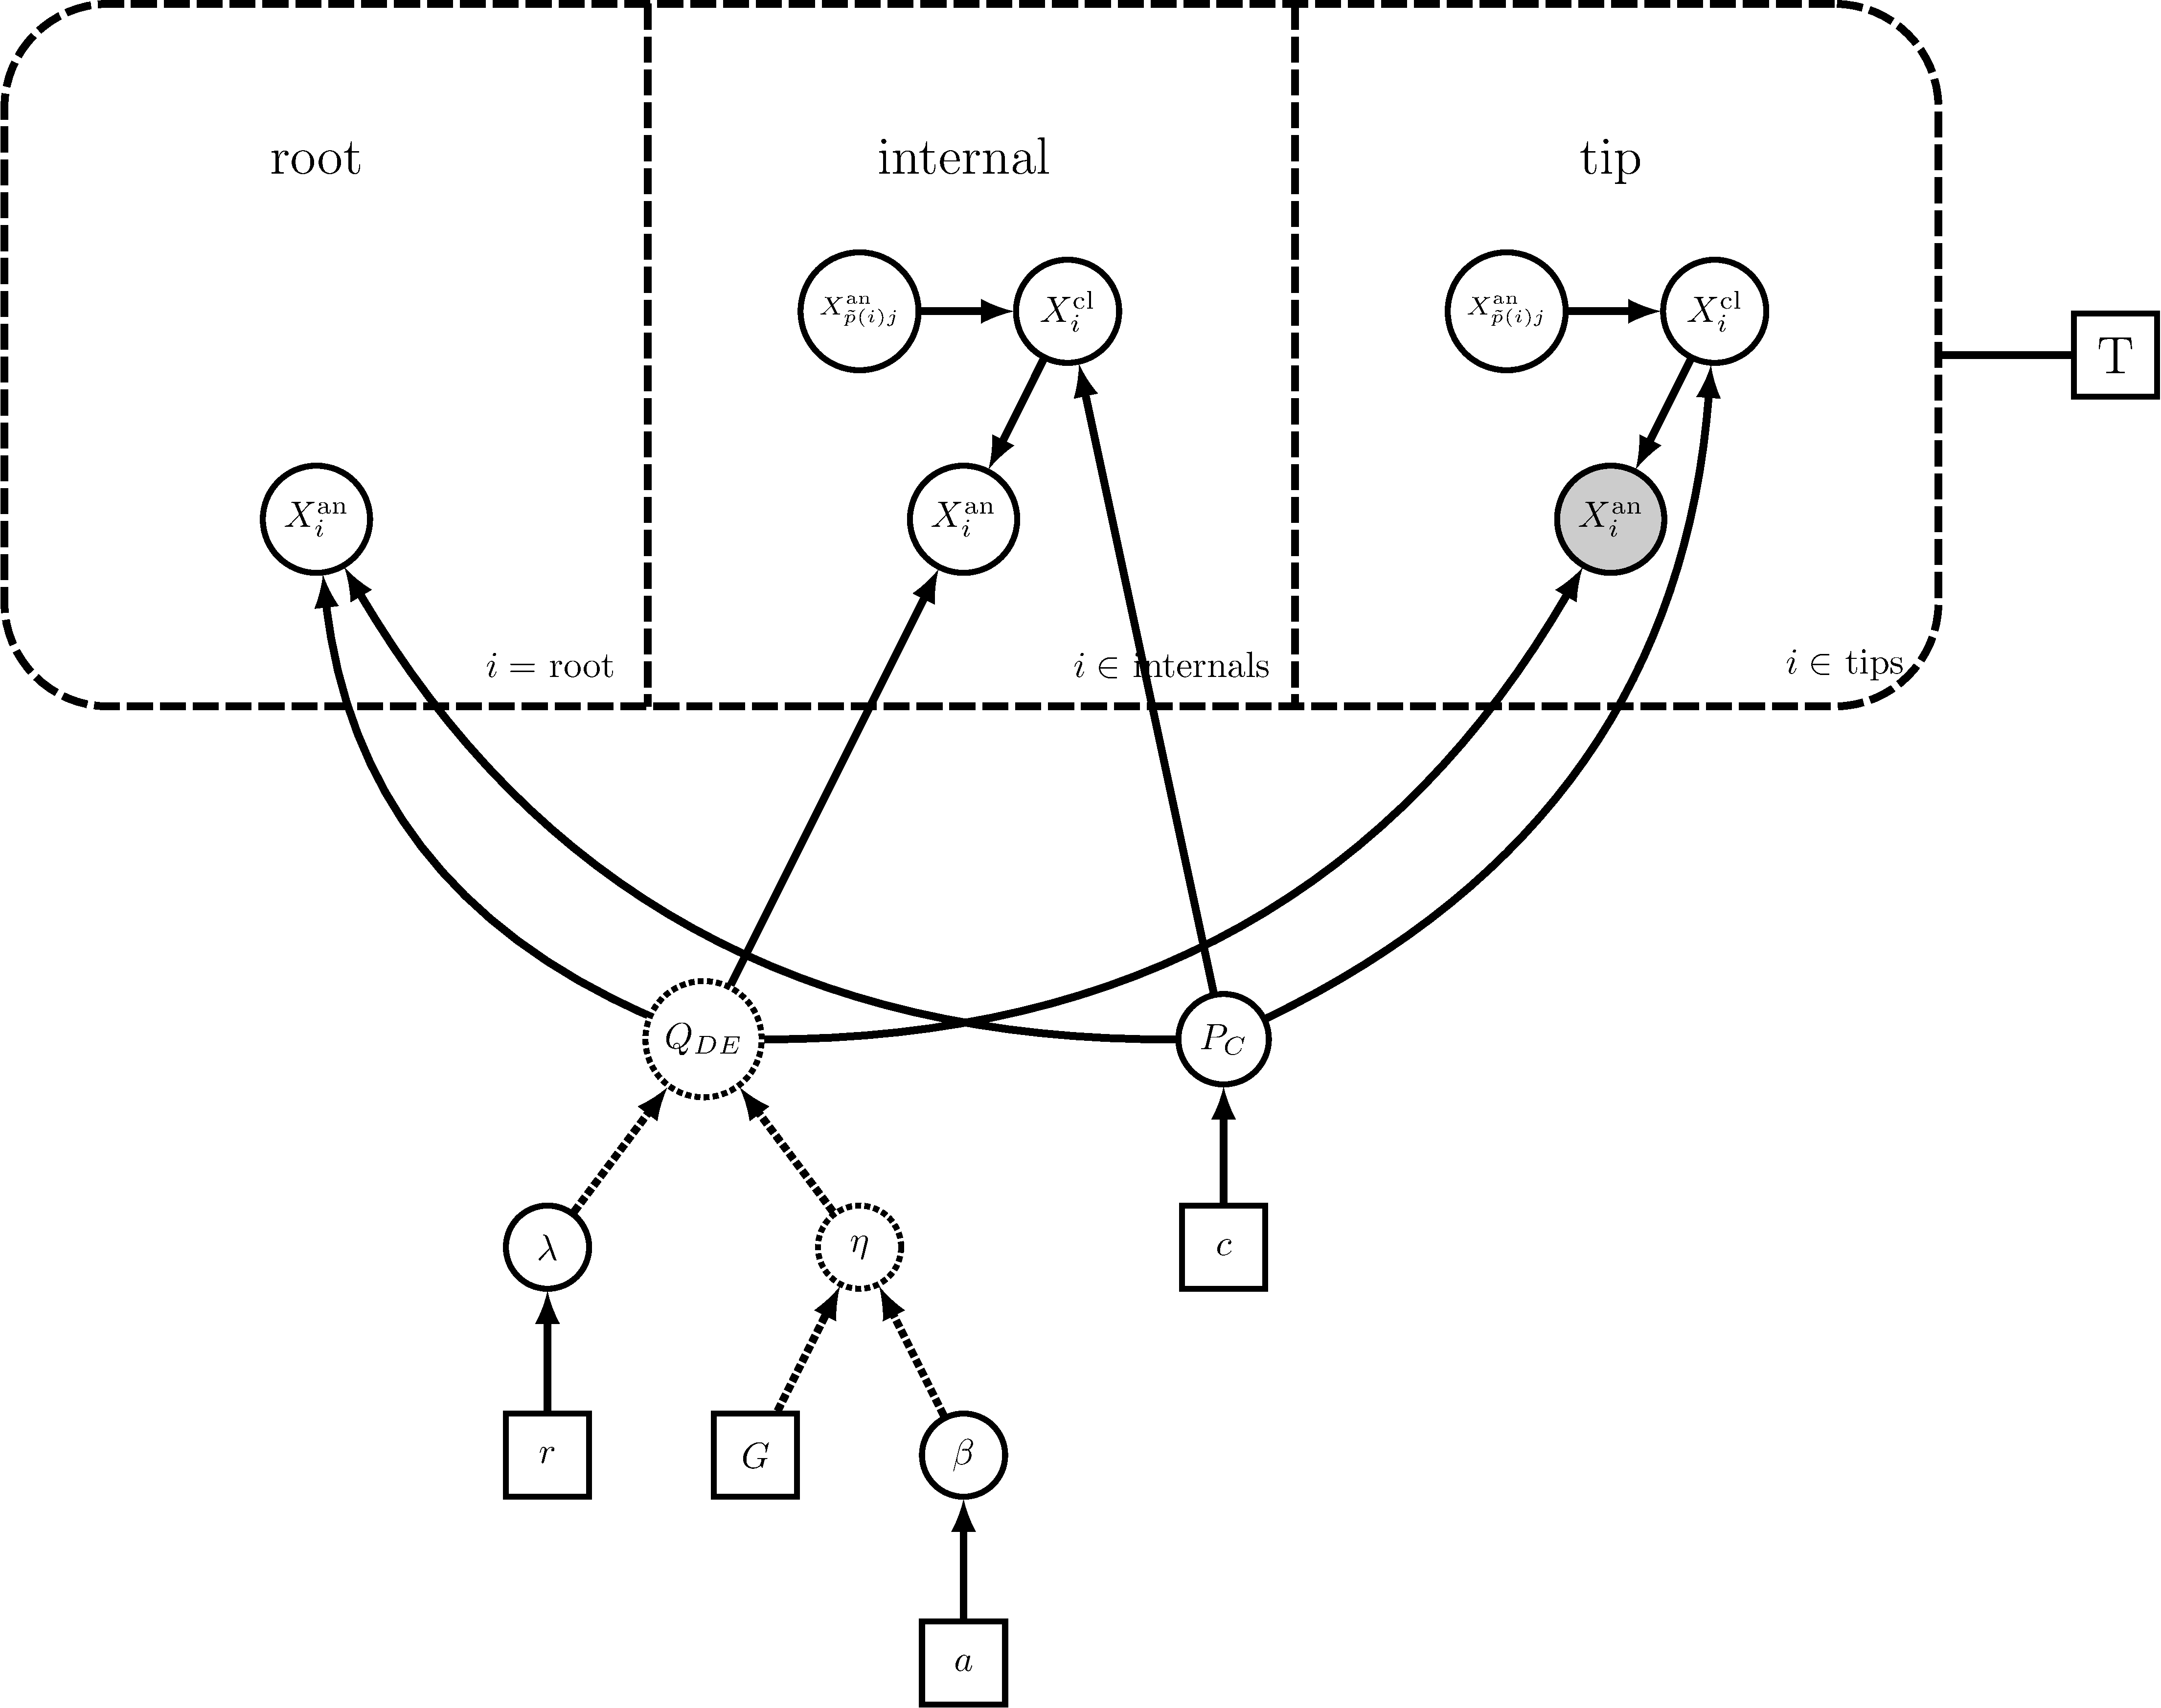
\includegraphics[width=5in]{RB_Biogeography_Tutorial/figures/bg_dec_dag}
\caption{Graphical model of DEC. The tree plate's topology is fixed by $T$, where each internal node has both an anagenic and cladogenic random variable ($X_i^{\text{an}}$ and $X_i^{\text{cl}}$, resp.) that represents an ancestral species before and after it speciated. Anagenic change is modeled by a continuous time Markov process, where $Q_{DE}$ is the instantaneous rate matrix of area gain and loss, as parameterized by $\lambda$. The geographic distance rate modifier function, $\eta$, takes in the geographical distances and strata as $G$, and the distance power parameter, $\beta$. Cladogenic change is modeled by $P_C$, a Dirichlet-distributed simplex with a flat prior.}
\end{figure}

Let's consider what happens to the size of \textbf{Q} when the number of areas, $N$, becomes large.
For three areas, \textbf{Q} is size $8 \times 8$.
For ten areas, \textbf{Q} is size $1024 \times 1024$, which approaches the largest size matrix that can be exponentiated in a practical amount of time.
This is problematic, meaning we need an alternative method to integrate over historical range evolution events.

You may wonder why matrix exponentiation works fine for molecular substitution models and large multiple sequence alignments.
Molecular substitution models typically assume each site in the multiple sequence alignment evolves independently, which may be justified because recombination degrades linkage disequilibrium over geological timescales.
Conveniently, this keeps \textbf{Q} small even for datasets with many sites.

Remember matrix exponentiation integrates over all \textit{unobserved} transition events during time $t$.
The likelihood of beginning in character $i$ and ending in character $j$ can be computed easily when the explicit series of event types and times are known.
While we will never know the exact history of events, we can use stochastic mapping in conjunction with Markov chain Monte Carlo (MCMC) to repeatedly sample range evolution histories that are consistent with the ranges observed in the study taxa at the tips of the phylogeny.
This technique is an adaptation of the data-augmented phylogenetic method first described by \citet{robinson03}, and was first applied to tertiary structure-dependent evolution of protein-coding nucleotide sequences.

This is the strategy we will use to infer the posterior distribution approximated is 
\newline{Prob$\left( \textbf{X}_{aug}, \theta \mid \textbf{X}_{obs}, T, M \right)$}, where $\textbf{X}_{obs}$ is the range data observed at the tips, $\textbf{X}_{aug}$ is the distribution of ancestral range reconstructions over the phylogeny, $T$, where $\textbf{X}_{aug}$ is inferred jointly with the parameters, $\theta$, assuming the range evolution model, $M$, that describes $\textbf{Q}$ above.
Ancestral range reconstructions are often of primary interest in phylogenetic biogeographic analyses, which are generated with support values as a by-product of the MCMC analysis.

The rest of this tutorial will describe how to assemble the input, run the analysis, assess the output, and visualize the results.

\newpage

%%%%%%%%%%%%%%%%
%%%%%%%%%%%%%%%%
\section{Input}

For this tutorial, we'll use a dataset for 19 species of $Psychotria$ whose range spans the Hawaiian archipelago.
The dataset was originally reported in \citet{nepokroeff03} and analyzed using the maximum likelihood method, LAGRANGE, by \citet{ree08}.
We'll use this dataset for three reasons.
First, it is relatively small, meaning we can produce results quickly.
Second, the Hawaiian archipelago can be broken into naturally discrete areas and has a well-characterized geographical history that is uncomplicated to model.
Third, it has previously been analyzed, which provides some basis for comparison to other methods.
To simplify things, this model will assume we live in a gentler world where presence-absence characters are known without error.

For larger datasets to play with, see {\tt input/sim\_aus\_50tip\_33area.*} for a simulated model where all cladogenic events were sympatric (wide and narrow only). 

\subsection{Nexus file}

The data file contains a matrix of binary characters corresponding to the observed ranges of the study taxa.

\noindent \\ \impmark  Open the file \texttt{examples/psychotria\_range.txt}.

\begin{framed}
\begin{lstlisting}
#NEXUS

begin data;
  dimensions ntax=19 nchar=4;
  format datatype=standard symbols = "01";
  matrix
    P_mariniana_Kokee2  1000
    P_mariniana_Oahu    0100
    ...
    P_hexandra_Oahu     0100
  ;
end;

Begin trees;
	TREE tree1 = ((((((((P_hawaiiensis_WaikamoiL1:0.9656850499,
	P_mauiensis_Eke:0.9656850499):0.7086257935,(P_fauriei2:1.23
	0218511,P_hathewayi_1:1.230218511):0.4440923324):0.17671155
	...
	89):0.4630447802,P_hexandra_Oahu:2.826939991):2.372081244);
End;
\end{lstlisting}
\end{framed}

Range data is stored in standard Nexus format.
In the {\tt data} block, the first line gives the dimensions of the data matrix and the second line indicates we will be using binary characters.
The four characters correspond to areas defined by the geography file (next subsection).
Rows in the {\tt matrix} block correspond to taxa and their range data, while columns give in which areas each taxon is present (1) or absent (0).
For example, taxon {\tt P\_hexandra\_Oahu} is present only in area 2.

The {\tt trees} block gives the tree describing the shared ancestry of the study species.
Because range evolution occurs in units of geological time, the analysis in this tutorial requires a high-quality time-calibrated phylogeny.
This typically requires a multiple sequence alignment over several loci plus fossils for calibration.
Since this data availability is often the limiting factor for which taxa to include for your analysis, it is best to produce the phylogeny first.
Only afterwards should you begin assembling data for your data matrix.
If your phylogeny cannot be calibrated (e.g. it has no fossils) your best alternative is to proceed with a time tree resulting from a divergence time estimation analysis.
For this tutorial, the phylogeny is assumed to contain no uncertainty.

\subsection{Atlas file}

The geography used in this tutorial represents the Hawaiian archipelago.
Beneath Hawaii, currently the largest and youngest island, is a volcanic hotspot that periodically creates new islands.
The ages of these islands are fairly well known, meaning we can model range availability as a function of time.
Following \citet{ree08}, we will lump groups of smaller islands into single areas to simplify the analysis, leaving us with four areas: Hawaii (H), Oahu (O), Maui (M; this includes Molokai and Lanai), and Kauai (K; this includes Niihau).
These areas are modeled have arisen 0.5, 1.9, 3.7, and 5.5 million years ago, respectively.

Although the model will use discrete-state biogeographic ranges, geographical area is naturally continuous.
This means we must impose some discretization upon the geography to designate a set of biogeographically meaningful characters called areas.
Different methods use different criteria for this discretization, so it is best to perform the discretization yourself rather than blindly using the discretization given from a previous study or method (but do blindly use the dataset included in this tutorial).
Some geographies have natural discretizations: for instance, the Hawaiian archipelago forms naturally discrete areas on the basis of islands.
For many geographies, however, it may unclear how to perform this discretization.
Much like morphological analyses, you might choose to choose areas based on expert opinion, based on some model, or using some ``naive'' uniform discretization.
This procedure is not part of the tutorial, but you should be aware that area definitions are not always obvious or objective.


\newpage

\noindent \\ \impmark  Open the file \texttt{examples/hawaii\_dynamic.atlas.txt}.

\begin{framed}
%\begin{lstlisting}[basicstyle=\tiny \listingsfont, columns=texcl]
\begin{lstlisting}
{
	"name":"HawaiianArchipelago5my",
	"epochs": [
		{
			"name":"epoch1",
			"start_age":100.0,
			"end_age":3.7,
			"areas":
			[{ "name":"Kauai",  "latitude":19.5667, "longitude": -155.5000, "dispersalValues": [ 1,0,0,0 ] },
			{ "name": "Oahu",   "latitude":19.5667, "longitude": -155.5000, "dispersalValues": [ 0,0,0,0 ] },
			{ "name": "Maui",   "latitude":19.5667, "longitude": -155.5000, "dispersalValues": [ 0,0,0,0 ] },
			{ "name": "Hawaii", "latitude":19.5667, "longitude": -155.5000, "dispersalValues": [ 0,0,0,0 ] }]
		},
		{
			"name":"epoch2",
			...
		},
		{
			"name":"epoch3",
			...
		},
		{
			"name":"epoch4",
			"start_age":0.5,
			"end_age":0.0,
			"areas":
			[{ "name":"Kauai",  "latitude":22.0833, "longitude": -159.5000, "dispersalValues": [ 1,1,1,1 ] },
			{ "name": "Oahu",   "latitude":21.4722, "longitude": -157.9772, "dispersalValues": [ 1,1,1,1 ] },
			{ "name": "Maui",   "latitude":20.8000, "longitude": -156.3333, "dispersalValues": [ 1,1,1,1 ] },
			{ "name": "Hawaii", "latitude":19.5667, "longitude": -155.5000, "dispersalValues": [ 1,1,1,1 ] }]
		}
	]
}
\end{lstlisting}
\end{framed}

This is called the Atlas file, which uses a file format called JSON.
JSON is a lightweight format used to assign values to variables in a hierarchical manner.
There are three main tiers to the hierarchy in the Atlas file: the atlas, the epoch, and the area.
In the lowest tier, each area corresponds to a character in the model and is assigned it's own properties.
In the middle tier, each epoch contains the set of homologous areas (characters) that may be part of a species' range, but importantly the properties of these areas may take on different values during different intervals of time, as given by the {\tt start\_age} and {\tt end\_age} variables.
Because the tree and range evolution model also operate on units of geological time, the rates of area gain and loss can condition on areas' properties as a function of time.
Sometimes these models are called stratified models or epochal models.
Finally, the atlas contains the array of epochs in the highest tier.

Each area is assigned a {\tt latitude} and {\tt longitude} to represent its geographical coordinates, ideally the area's centroid.
If a centroid does not represent the distance between areas, splitting the area into multiple smaller areas is reasonable.
The data augmentation approach used in this analysis allows you to use more areas as desired, whereas matrix exponentiation methods are limited to approximately ten areas.
The distance between any two areas' coordinates inform to distance-dependent dispersal parameter ($\beta$ from the $\eta(\cdot)$ function) for range expansion events, so coordinates roughly close to the center of the area suffice.
Here, the {\tt latitude} and {\tt longitude} change in each of the four epochs, where they begin at the current location of Hawaii and drift northwesterly until they reach their current positions.

In addition, each area is marked as habitable or not using the {\tt dispersalValues} array.
The elements in the array correspond to the other areas defined in the analysis.
For example, in {\tt epoch1}, Kauai's {\tt dispersalValues} is equal to {\tt [ 1,0,0,0 ]}, which indicates Kauai exists at that point in time but it is not in contact with any other areas, i.e. the range in that area cannot expand into other areas.
The {\tt dispersalValues} for Oahu, Maui, and Hawaii are all equal to {\tt [ 0,0,0,0 ]}, meaning no species may be present in that area during the time interval of {\t epoch1} during ages from 10.0 to 3.7. In contrast, {\tt epoch4}, from ages 0.5 to the present, range expansions may occur between any pair of areas and any area may be included in a species' range.

\section{RevBayes Analysis}

There are six major parts to the analysis.

First, we need to read in the input files and assign analysis settings.
Second, we need to construct our model.
Third, we need to assign moves and monitors to our model parameters for use with Markov chain Monte Carlo (MCMC).
Fourth, we will run an MCMC analysis assuming a complex model.
Fifth, we will compare the complex model with a simple model using Bayes factors.
Finally, we'll analyze our MCMC output.

\subsection{Analysis settings}

\setlength{\parindent}{0pt}

\noindent \\ \impmark Open the RevBayes console

\begin{snugshade}
\begin{lstlisting}
$ revbayes
\end{lstlisting}
\end{snugshade}

First, we'll assign all our input files to {\tt String} variables.
\begin{snugshade}
\begin{lstlisting}
RevBayes > in_fp   <- "./input/"
RevBayes > data_fn <- "psychotria_range.nex"
RevBayes > area_fn <- "hawaii_dynamic.atlas.txt"
RevBayes > out_fp  <- "./output/"
RevBayes > out_str <- "bg_2rate"
\end{lstlisting}
\end{snugshade}

Then we'll create our range data, tree, and atlas objects

\begin{snugshade}
\begin{lstlisting}
RevBayes > data  <- readDiscreteCharacterData(in_fp + data_fn)
RevBayes > tree  <- readTrees(in_fp + data_fn)[1]
RevBayes > atlas <- readAtlas(in_fp + area_fn)
\end{lstlisting}
\end{snugshade}

%Verify the data and tree share the same number of taxa and the data and atlas share the same number of characters
%
%\begin{snugshade}
%\begin{lstlisting}
%RevBayes > data.ntaxa() == tree.ntips()
%   true
%RevBayes > data.nchar() == atlas.nareas()
%   true
%\end{lstlisting}
%\end{snugshade}


\subsection{Creating the model}

Here, we will compose our rate matrix, {\bf Q}, parameterized by the transition rates, $\lambda$, and the distance dependent dispersal power parameter, $\beta$.

First, for $\lambda$, we will create a vector of two rates, where {\tt glr[1]} corresponds to the rate of area loss (local extinction) and {\tt glr[2]} corresponds to the rate of area gain (dispersal).
Each rate will be drawn from an exponential distribution with rate 10.0 (mean 0.1).
Because our tree is in units of millions of years, this means our prior expectation is that any given species undergoes one dispersal or extinction event per area per ten million years.

To introduce this to the model, type
\begin{snugshade}
\begin{lstlisting}
RevBayes > for (i in 1:2) glr[i] ~ dnExponential(10.0)
\end{lstlisting}
\end{snugshade}

Next, we will create {\tt dp}, which determines the importance of geographical distance to dispersal.
Remember that values of $\beta$ far from zero means distance is important.
So, if we we assign a prior that pulls $\beta$ towards zero, then posterior values of $\beta$ far from zero indicate the range data are informative of the importance of distance to dispersal.
We'll use an exponential distribution with rate 10.0 (mean 0.1) as a prior for {\tt dp}.

We will also create a deterministic node to modify the rate of dispersal between areas by evaluating {\tt dp} and {\tt atlas}.
This node is determined by the function {\tt fnBiogeoGRM}, where GRM stands for ``geographical rate modifier'', and plays the role of the $\eta(\cdot)$ rate-modifier function mentioned earlier.
We will tell the {\tt fnBiogeoGRM} function to modify dispersal rates based on distances and whether or not the area exists during an epoch.

\begin{snugshade}
\begin{lstlisting}
RevBayes > dp ~ dnExponential(10.0)
RevBayes > grm := fnBiogeoGRM(atlas=atlas, distancePower=dp, useAvailable=true, useDistance=true)
\end{lstlisting}
\end{snugshade}

Now we need a deterministic node to represent the rate matrix, {\bf Q}.
To determine the value of this node, we'll use the function {\tt fnBiogeoDE} to assign our model parameters to transition rates as described in the introduction.
As input, we'll pass our gain and loss rates, {\tt glr}, and our geographical rate modifier, {\tt grm}.
In addition, we'll inform the function of the number of areas in our analysis and whether we will allow species to be absent in all areas (i.e. have the null range).

\begin{snugshade}
\begin{lstlisting}
RevBayes > Q := fnBiogeoDE(gainLossRates=glr, geoRateMod=grm, numAreas=4, forbidExtinction=true)
\end{lstlisting}
\end{snugshade}

To extract information for the frequencies of different cladogenic event types, we will create a Dirichlet-distributed stochastic node.
The simplex is over three events, subset sympatry (index 0), allopatry (index 1), and widespread sympatry (index 2), but not over narrow sympatry whose range size is one.
The prior parameter {\tt [1,1,1]} is known as a flat prior, meaning all event types are expected to occur at equal frequency.
If there is information in the data of a dominant cladogenic mode of range evolution, the posterior simplex values in {\tt csf} will reflect this.

\begin{snugshade}
\begin{lstlisting}
RevBayes > csf ~ dnDirichlet([1,1,1])
\end{lstlisting}
\end{snugshade}

For the model's final node, we create the stochastic node for the continuous-time Markov chain (CTMC).
This node's distribution is {\tt dnPhyloDACTMC} where {\tt DA} indicates the CTMC uses data-augmentation to compute the likelihood rather than Felsenstein's pruning algorithm.
To create the distribution, we must pass it our {\tt tree} and {\tt Q} objects, but additionally inform the distribution that it will be using a biogeographic model, that it will introduce the simple cladogenic range evolution events described in \citet{ree08} ({\tt useCladogenesis=true}), and that it will assign zero probability to a transition away from the null range state.

\begin{snugshade}
\begin{lstlisting}
RevBayes > M ~ dnPhyloDACTMC(tree=tree, Q=Q, C=csf, type="biogeo", forbidExtinction=true, useCladogenesis=true)
\end{lstlisting}
\end{snugshade}

So we may evaluate the graphical model's likelihood, we tell the CTMC to observe the {\tt data} object, which will prime the model with data-augmented character histories.
Now {\tt M} has a defined likelihood value.
\begin{snugshade}
\begin{lstlisting}
RevBayes > M.clamp(data)
RevBayes > M.lnProb
   -56.0288
\end{lstlisting}
\end{snugshade}

Finally, we encapsulate our graphical model into a {\tt Model} object, which can learn the model's structure and dependencies from any model parameter.
\begin{snugshade}
\begin{lstlisting}
RevBayes > my_model <- model(glr)
\end{lstlisting}
\end{snugshade}

\subsection{Running an MCMC analysis}

Now that we have our {\tt Model} object, we can soon run an MCMC analysis.
Remember that MCMC approximates the posterior distribution by repeatedly proposing new model parameter values, accepting or rejecting those new parameter values based on the model likelihood (and on biases in the proposal distribution), then reporting the sampled parameter values.

First, let's assign moves to our model parameters.
These parameters are all supported for real positive values, which is appropriate for use with scale-multipler proposal, {\tt mvScale()}.
To inspect our model parameter types and the proposal argument types, enter

\begin{snugshade}
\begin{lstlisting}
RevBayes > type(dp)
   RealPos
RevBayes > type(glr)
   RealPos[]
RevBayes > mvScale
   Move_Scale function (RealPos x, RealPos lambda, Bool tune, RealPos weight)
\end{lstlisting}
\end{snugshade}

The arguments for {\tt mvScale} are fairly typical as far as RevBayes {\tt Move} objects go: {\tt x} is the stochastic node the {\tt Move} will update, {\tt lambda} is proportional to how radically different proposed parameter values will tend to be, {\tt tune} allows {\tt lambda} to be adjusted automatically as the MCMC runs, and {\tt weight} tells the MCMC how many times to perform the {\tt Move} during a single MCMC generation (e.g., {\tt weight=2.0)} means each generation will call that {\tt Move} for the parameter {\tt x} twice).


\begin{snugshade}
\begin{lstlisting}
RevBayes > moves[1] <- mvScale(x=glr[1], lambda=0.5, tune=false, weight=5.0)
RevBayes > moves[2] <- mvScale(x=glr[2], lambda=0.5, tune=false, weight=5.0)
RevBayes > moves[3] <- mvScale(x=dp, 	 lambda=0.5, tune=false, weight=5.0)
RevBayes > moves[4] <- mvSimplexElementScale(csf, alpha=10.0, tune=false, weight=4.0)
\end{lstlisting}
\end{snugshade}

In addition to proposing new model parameter values, we must also propose new data-augmented states and events to properly integrate over the space of possible range histories.
The major challenge to sampling character histories is ensuring the character histories are consistent with the observations at the tip of the tree.
The proposals in this tutorial use \citet{nielsen02}'s rejection sampling algorithm, with some modifications to account for cladogenic events and epoch-based rate matrices.

The basic idea is simple.
Each time a character history proposal is called, it selects a node at random from the tree.
Path history proposals ({\tt mvPathCHRS()}) propose a new character history for the lineage leading to that node.
Node history proposals ({\tt mvNodeCHRS()}) propose a new character history for the node and for the three lineages incident to that node.
The character history proposal also samples some number of areas to update, ranging from one to all of the areas.
Once the new character history is proposed, the likelihood of the model is evaluated and the MCMC accepts or rejects the new state according to e.g. the Metropolis-Hastings algorithm.

Because these {\tt Move} objects update the character histories stored in the data-augmented CTMC node, e.g. {\tt M},
they require access to a {\tt TimeTree} object to know which lineages are sisters and whether the lineages span various epochs, and a {\tt RateMap\_Biogeography} object to propose new character histories.
The {\tt lambda} argument gives what proportion of areas' character histories to update.
Here, if {\tt lambda=0.2}, then the proposal will redraw character histories for each area with probability 0.2 (in addition to one random area with probability 1).
Below, we use two moves of each type with {\tt lambda=0.2} and {\tt lambda=1.0} for partial and full character history updates, respectively.
Indicating {\tt type="biogeo"} informs the {\tt Move} object to be aware of special character history constraints, such as cladogenic events and forbidden null ranges.
The {\tt weight} parameter should be assigned a value proportional to the number of nodes in the analysis to ensure proper mixing.

Let's create the character history moves as follows.

\begin{snugshade}
\begin{lstlisting}
RevBayes > n_nodes  <- tree.nnodes()
RevBayes > moves[5] <- mvNodeCHRS(ctmc=M, qmap=Q, tree=tree, lambda=0.2, type="biogeo", weight=2.0*n_nodes)
RevBayes > moves[6] <- mvPathCHRS(ctmc=M, qmap=Q, tree=tree, lambda=0.2, type="biogeo", weight=2.0*n_nodes)
RevBayes > moves[7] <- mvNodeCHRS(ctmc=M, qmap=Q, tree=tree, lambda=1.0, type="biogeo", weight=n_nodes)
RevBayes > moves[8] <- mvPathCHRS(ctmc=M, qmap=Q, tree=tree, lambda=1.0, type="biogeo", weight=n_nodes)
\end{lstlisting}
\end{snugshade}

Now that we have moves for all our parameters and the character histories, we'll proceed with assigning {\tt Monitor} objects to record their values.
The first two {\tt Monitor} objects are fairly standard and found in most RevBayes MCMC analyses.
{\tt mnScreen} reports the values for any nodes assigned to {\tt RevObject ...} every {\tt printgen} generations to the terminal screen.
{\tt mnModel} reports the values for all nodes in the {\tt Model} object every {\tt printgen} generations to the file assigned to {\tt filename}, which is delimited by the {\tt separator} character.

\begin{snugshade}
\begin{lstlisting}
RevBayes > mnScreen
   Mntr_Screen function (RevObject ..., Natural printgen, Bool posterior, Bool
   likelihood, Bool prior)
RevBayes > monitors[1] <- mnScreen(printgen=10, glr, dp, csf)
RevBayes > mnModel
   Mntr_Model function (String filename, Natural printgen, String separator,
   Bool posterior, Bool likelihood, Bool prior, Bool append, Bool
   stochasticOnly)
RevBayes > monitors[2] <- mnModel(filename=out_fp+params_fn, printgen=10)
\end{lstlisting}
\end{snugshade}

Like any parameter, we can sample the augmented range histories from the MCMC to approximate the posterior distribution of range histories.
This is statistically equivalent to generating ancestral state reconstructions from a posterior distribution via stochastic mapping.
We will extract these reconstructions using special monitors designed for the {\tt dnPhyloDACTMC} distribution.

Next, we will create {\tt Mntr\_CharacterHistoryNewickFile} objects to record the sampled character history states for each node in the tree.
This {\tt Monitor} has two {\tt style} options: {\tt counts} reports the number of gains and losses per branch in a tab-delimited Tracer-readable format;  {\tt events} reports richer information of what happens along a branch, anagenically and cladogenically, using an extended Newick format.
How to read these file formats will be discussed in more detail in Section \ref{sec:posterior}.

\begin{snugshade}
\begin{lstlisting}
RevBayes > mnCharHistoryNewick
   Mntr_CharacterHistoryNewickFile function (String filename,
   AbstractCharacterData ctmc, TimeTree tree, Natural printgen, String
   separator, Bool posterior, Bool likelihood, Bool prior, Bool append, String
   style = events|counts
   , String type = biogeo
   )
RevBayes > monitors[3] <- mnCharHistoryNewick(filename=fp+out_str+".events.txt", ctmc=M, tree=tree, printgen=100, style="events")
RevBayes > monitors[4] <- mnCharHistoryNewick(filename=fp+out_str+".counts.txt", ctmc=M, tree=tree, printgen=100, style="counts")
\end{lstlisting}
\end{snugshade}

As our last monitor, the {\tt Mntr\_CharacterHistoryNhxFile} records character history values throughout the MCMC analysis, then stores some simple posterior summary statistics as a Nexus file.
These summary statistics could be computed from the previously mentioned {\tt Monitor} output files, but {\tt mnCharHistoryNhx} provides a simple way to produce Phylowood-compatible files.
We will also discuss this file's format in more detail later in the tutorial.

\begin{snugshade}
\begin{lstlisting}
RevBayes > mnCharHistoryNhx
   Mntr_CharacterHistoryNhxFile function (String filename, AbstractCharacterData
   ctmc, TimeTree tree, RlAtlas atlas, Natural samplegen, Natural maxgen,
   Probability burnin, String separator, Bool posterior, Bool likelihood, Bool
   prior, String type = biogeo
   )
RevBayes > monitors[5] <- mnCharHistoryNhx(filename=fp+out_str+".nhx.txt", ctmc=M, tree=tree, atlas=atlas, samplegen=100, maxgen=25000, burnin=0.2)
\end{lstlisting}
\end{snugshade}

Before we run the MCMC, we'd like to get the node index of the ancestor 
When analysing the output, we'll take some special interest in the branch for the most recent common ancestor of {\it P. kaduana} and {\it P. hatheway}.
We will identify this lineage by its index, 23, which is meaningful only for a fixed tree topology,
\begin{snugshade}
\begin{lstlisting}
RevBayes > names = tree.names()
RevBayes > names[15]
   P_kaduana_PuuKukuiAS
RevBayes > names[16]
   P_hathewayi_1
RevBayes > mrcaIndex(tree=tree,clade=clade(names[15],names[16]))
   23
\end{lstlisting}
\end{snugshade}


\subsection{Running an MCMC analysis}

Now all that's left is to configure and run our MCMC analysis.
For this, we create an {\tt Mcmc} object, which we give our {\tt Move} vector, our {\tt Monitor} vector, and our {\tt Model object}

\begin{snugshade}
\begin{lstlisting}
RevBayes > mcmc
   MCMC function (Model model, Monitor[] monitors, Move[] moves, String
   moveschedule = sequential|random|single
   )
RevBayes > my_mcmc <- mcmc(my_model, monitors, moves)
\end{lstlisting}
\end{snugshade}

MCMC typically requires some period of burn-in before it reaches stationarity, i.e. from a random starting point, it takes some time for the chain to produce valid samples from the posterior distribution.
By running {\tt burnin()}, we tell the {\tt Mcmc} object to propose and reject new states but {\it not} to record anything to file.
After burn-in is complete, we call {\tt run()}, where we begin recording valid posterior samples under our model.

\begin{snugshade}
\begin{lstlisting}
RevBayes > my_mcmc.burnin(generations=1000, tuningInterval=50)
RevBayes > my_mcmc.run(generations=25000)
\end{lstlisting}
\end{snugshade}

Everything we've done is contained in the file {\tt biogeography\_DEC\_2rate.Rev}.
You can modify this file as you like then re-run the analysis by typing

\begin{snugshade}
\begin{lstlisting}
RevBayes > source("./scripts/biogeography_DEC_2rate.Rev")
\end{lstlisting}
\end{snugshade}

\subsection{Model selection using Bayes factors}

Bayes factors (BFs) are used to select which of two models better describes the observed data, $\mathbf{X}_{obs}$, and are computed as the ratio of marginal likelihoods for those two models.
One might prefer to analytically compute the marginal likelihood, but it's the same intractable quantity we intentionally avoid computing when using MCMC in a Bayesian context.
Instead, we must estimate the marginal likelihood from our posterior distribution samples.
Here, we will use thermodynamic integration \citep{lartillot06} and stepping-stone approximation \citep{xie10}.
The exact details of these techniques will not be covered here, but there is an important practical point to mention: both methods rely on computing a number of ``power posterior'' distributions.
Computing more power posteriors increases the marginal likelihood estimator's accuracy at the cost of computational time.

Moving on, we'll compute the Bayes factor to compare a simple one-rate model, which asserts the rate of area gain and loss are always equal, to a two-rate model which allows these rates to vary independently.
Rather than specifying the model manually, we will load (source) the model definition from a file then enter the commands to compute its marginal likelihood.
For faster results, we will use two separate RevBayes sessions, one for each model.
For each session, the power posterior analysis run for 1000 generations during burn-in then 1000 generations per each of 30 power posterior categories.

First session:
\begin{snugshade}
\begin{lstlisting}
RevBayes > source("./scripts/biogeography_DEC_1rate.Rev")
RevBayes > pp_fn <- out_fp + out_str + ".pp.txt"
RevBayes > pow_p <- powerPosterior(my_model, moves, pp_fn, cats=30) 
RevBayes > pow_p.burnin(generations=1000,tuningInterval=100)
RevBayes > pow_p.run(generations=5000)
\end{lstlisting}
\end{snugshade}

Second session:
\begin{snugshade}
\begin{lstlisting}
RevBayes > source("./scripts/biogeography_DEC_2rate.Rev")
RevBayes > pp_fn <- out_fp + out_str + ".pp.txt"
RevBayes > pow_p <- powerPosterior(my_model, moves, pp_fn, cats=30) 
RevBayes > pow_p.burnin(generations=1000,tuningInterval=100)
RevBayes > pow_p.run(generations=5000)  
\end{lstlisting}
\end{snugshade}

Each power posterior analysis will write their contents to the file given in {\tt pp\_fn}.
These files are {\tt bg\_1rate.pp.txt} and {\tt bg\_2rate.pp.txt} for the simple and complex models, respectively.
This may take a few minutes.
When complete, the power posterior files may then be used to compute marginal likelihoods.
For example, from the RevBayes session analyzing the simple one-rate model

\begin{snugshade}
\begin{lstlisting}
RevBayes > ss <- steppingStoneSampler(file=pp_fn)
RevBayes > ss.marginal() 
RevBayes > ps <- pathSampler(file=pp_fn)
RevBayes > ps.marginal() 
\end{lstlisting}
\end{snugshade}

For a given model, the path sampling and stepping stone sampling methods should produce similar marginal likelihood estimates.
Values should be within one log likelihood unit of one another.
If the values are extremely different, this may indicate {\tt powerPosterior} should be re-run with a larger number of {\tt cats}.
We chose {\tt cats=30} which should suffice, and we see no problem.
Then from the complex two-rate model RevBayes session using the same commands as above.
Finally, we can compute the Bayes factor, which is simply the ratio of marginal likelihoods.

\begin{snugshade}
\begin{lstlisting}
RevBayes > exp(-51.7202)/exp(-52.3158)
   1.81412
\end{lstlisting}
\end{snugshade}

A value of one would mean both models had equal marginal likelihoods.
A value less than one would indicate the first model, the simple model, had a larger marginal likelihood, and was therefore favored by model testing.
But that's not the case, the value is greater than one, and the complex two-rate model is favored.
Similar to frequentist interpretations of significance for p-values, there is no universal and objective criterion of significance with Bayes factors, but most would agree a factor of 1.8 (or 1.0/1.8) indicates weak support for one model over the other.

\section{Output}

\subsection{Sampled parameters from {\tt ScreenMonitor}}

The {\tt mnScreen} monitor reports model parameter values to the screen, where each row corresponds to the current accepted MCMC state, and each column reports some model feature, such as the model likelihood or a parameter value.
Every 20 iterations, this monitor re-prints the column headers.

\begin{snugshade}
%\begin{lstlisting}[basicstyle=\tiny \listingsfont, columns=texcl]
\begin{lstlisting}
RevBayes > my_mcmc.run(generations=25000)

Running MCMC simulation for 25000 iterations
The simulator uses 8 different moves in a random
move schedule with 241 moves per iteration

Iteration   |   Posterior  |          dp  |      glr[1]  |      glr[2]  |      csf[1]  |      csf[2]  |      csf[3]
-------------------------------------------------------------------------------------------------------------------
0           |    -51.3307  |   0.0570518  |    0.175137  |   0.0580957  |    0.330891  |    0.255308  |    0.413801
10          |    -54.4257  |   0.0416423  |    0.166936  |    0.178402  |   0.0549136  |    0.148854  |    0.796233
20          |    -58.0696  |   0.0991853  |    0.136495  |    0.122135  |    0.308418  |    0.448892  |    0.242689
30          |    -46.5049  |     0.10676  |   0.0958918  |   0.0959592  |    0.543837  |    0.363871  |   0.0922922
40          |    -42.8697  |    0.173549  |    0.158565  |   0.0662419  |    0.569416  |    0.126439  |    0.304145
50          |    -43.5319  |    0.117868  |    0.196497  |   0.0523307  |    0.440269  |    0.257171  |     0.30256

...
\end{lstlisting}
\end{snugshade}

For the complex 2-rate model, our model parameters are {\tt dp}, the distance power parameter, and the rates of area loss and gain, {\tt glr[1]} and {\tt glr[2]}, respectively, and the frequencies for subset sympatry, allopatry, and widespread sympatry {\tt csf[1]}, {\tt csf[2]}, and {\tt csf[3]}, respectively. 
If you notice the value of some parameter is rarely updated from iteration to iteration, the MCMC is probably mixing poorly therefore it's not generating samples from the posterior distribution (the MCMC's stationary distribution).
In this case, you may want to re-run the analysis with different arguments for the {\tt Move} object assigned to that parameter.

\subsection{Sampled parameters from {\tt ModelMonitor}}

This tab-delimited file contains parameter samples from the posterior distribution.
As with the {\tt ScreenMonitor}, columns are model or parameter values and rows are MCMC cycles.

\begin{framed}
%\begin{lstlisting}[basicstyle=\tiny \listingsfont, columns=texcl]
\begin{lstlisting}
Iteration  Posterior  Likelihood    Prior  glr[1]  glr[2]  dp  csf[1]  csf[2]  csf[3]
0           -51.3307    -56.0288  4.69806  0.175137  0.0580957  0.057051  0.330891  0.255308  0.413801
10          -54.4257    -58.1568  3.73110  0.166936  0.1784020  0.041642  0.054913  0.148854  0.796233
20          -58.0696    -62.0923  4.02274  0.136495  0.1221350  0.099185  0.308418  0.448892  0.242689
30          -46.5049    -51.1197  4.61480  0.095891  0.0959592  0.106760  0.543837  0.363871  0.092292
40          -42.8697    -46.4870  3.61735  0.158565  0.0662419  0.173549  0.569416  0.126439  0.304145
50          -43.5319    -47.4659  3.93394  0.196497  0.0523307  0.117868  0.440269  0.257171  0.302560

...
\end{lstlisting}
\end{framed}

\noindent \\ \impmark Open Tracer, select the fields for the posterior probability and area gain rate, {\tt glr[2]}, then click the Joint-Marginal tab.

\begin{figure}[H]
\centering
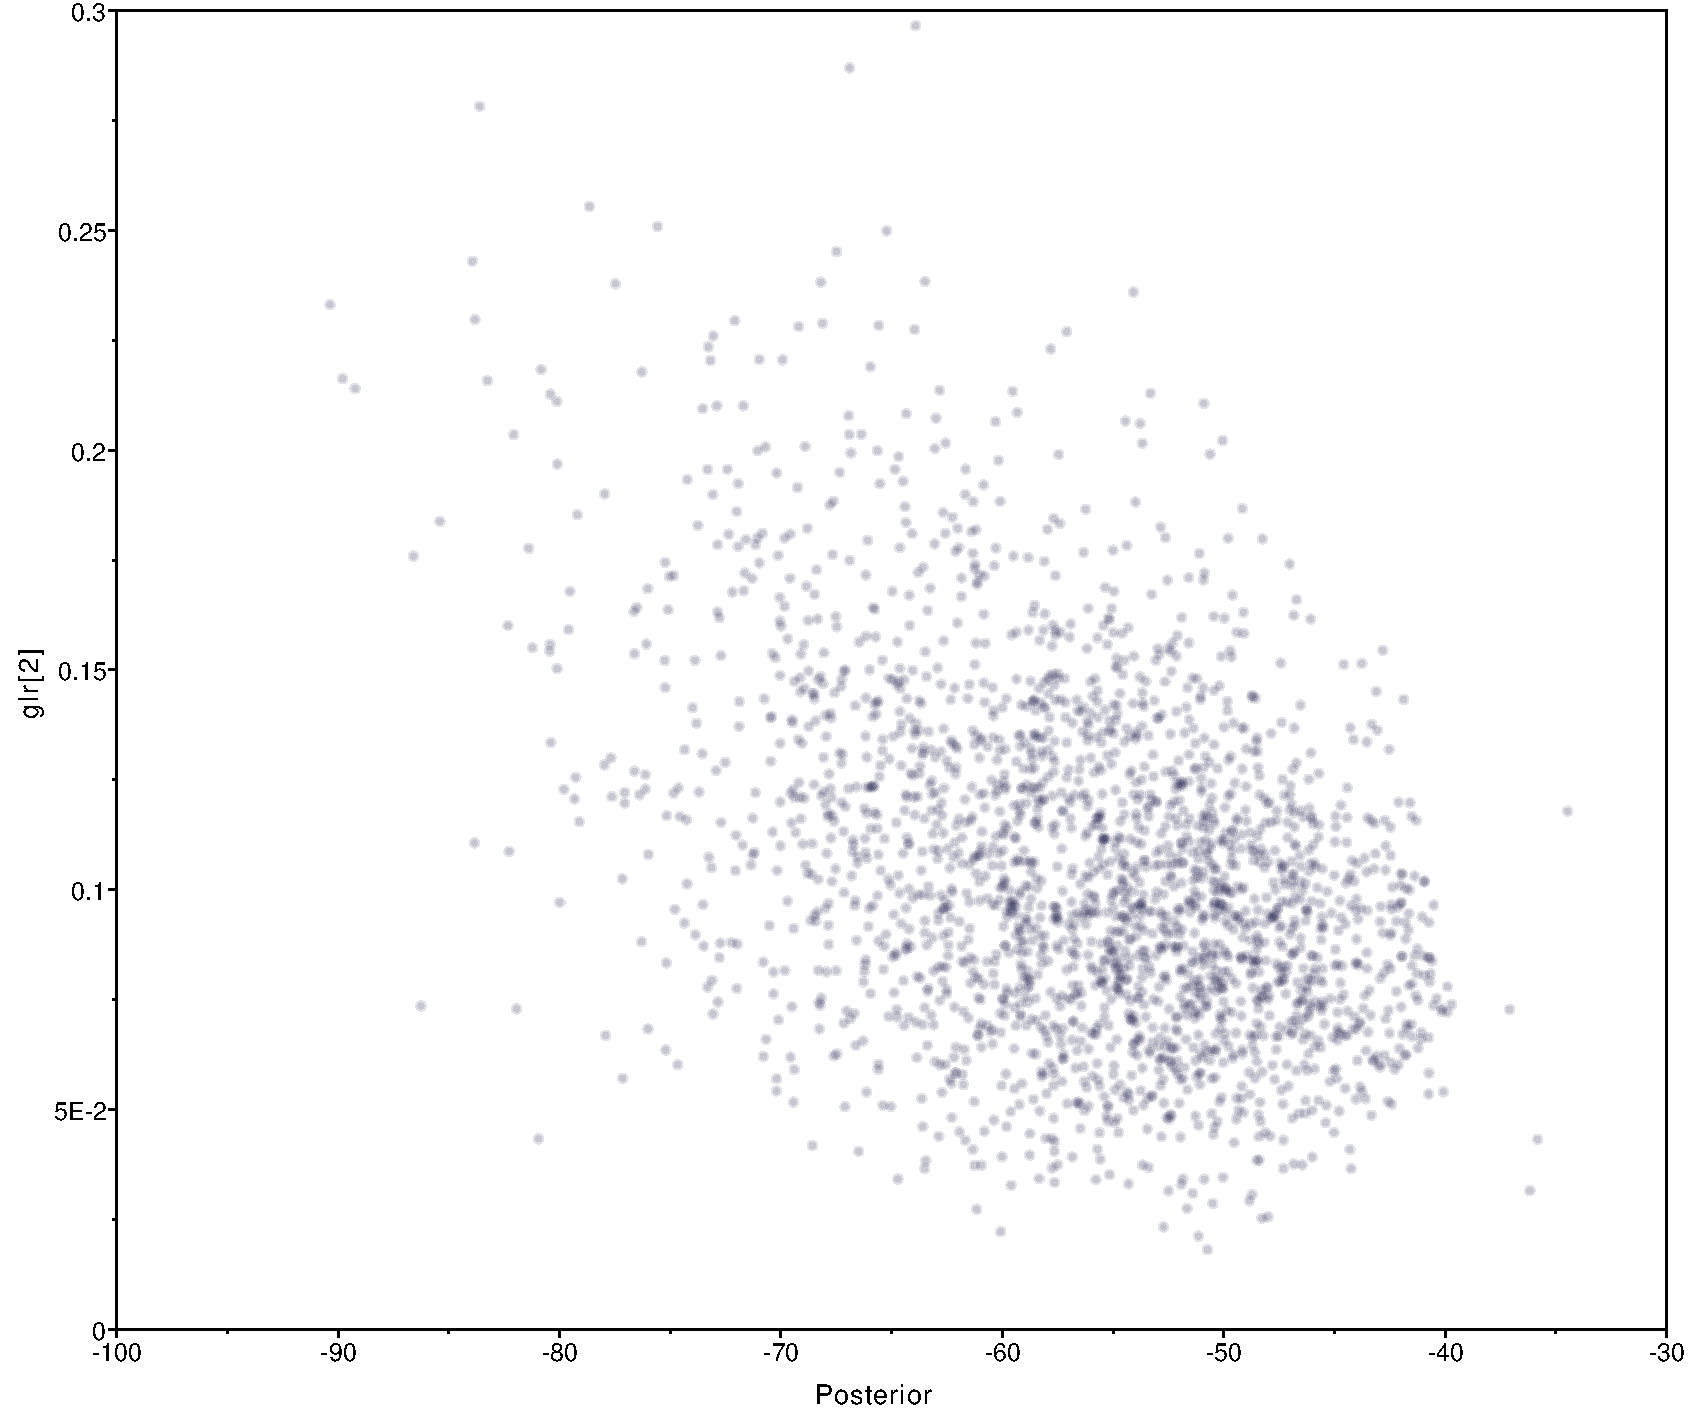
\includegraphics[width=3in]{RB_Biogeography_Tutorial/figures/joint_rgain_posterior}
\caption{Joint-marginal distribution of posterior and area gain rate, $\lambda_1$.}
\end{figure}

Here, we see a strong negative correlation between the posterior probability and the area gain rate, which is expected.
Next, click the Estimates tab then select the three {\tt csf} parameters.

\begin{figure}[H]
\centering
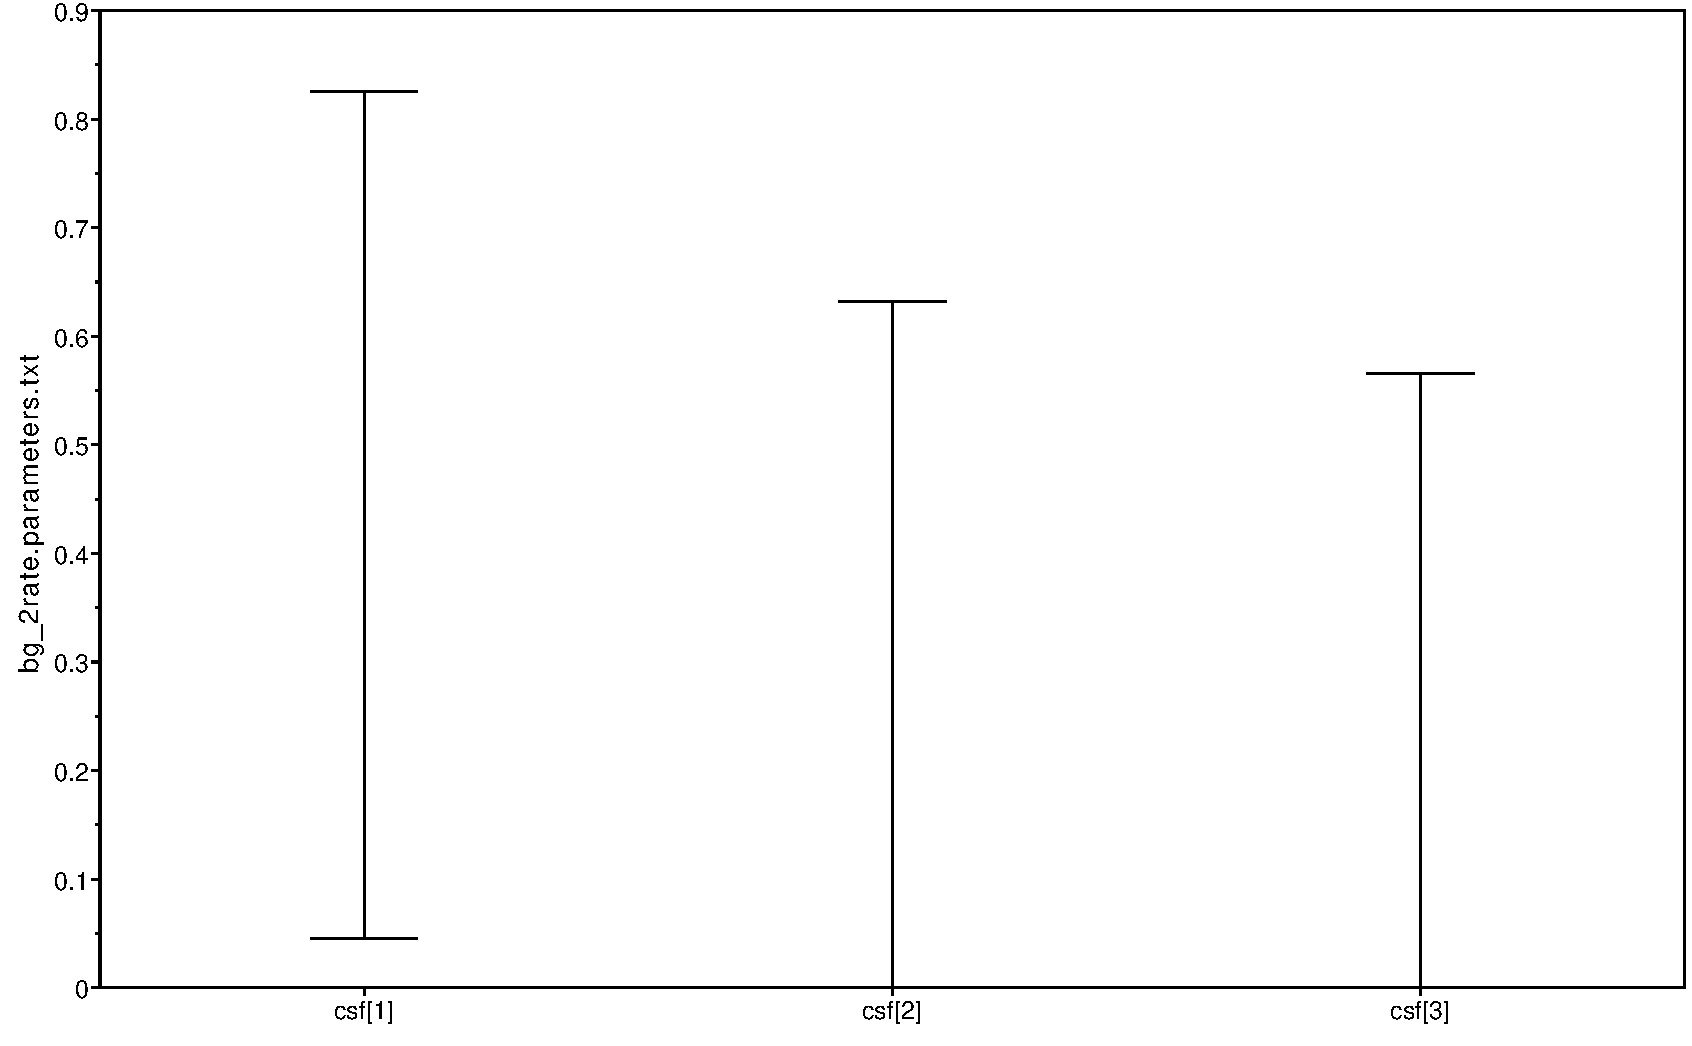
\includegraphics[width=3in]{RB_Biogeography_Tutorial/figures/clado_freq_posterior}
\caption{Mean values for the cladogenic state frequency simplex, where {\tt csf[1]}, {\tt csf[2]}, and {\tt csf[3]} correspond to subset sympatry, allopatry, and wide sympatry whose mean posterior values are 0.45, 0.30, and 0.25, respectively.}
\end{figure}


\subsection{Biogeographic event counts from {\tt mnCharHistoryNewick}}

Recording stochastic mappings in a Tracer-compatible format requires some summarization.
This monitor generates a tab-delimited file where the number of events of each type for each branch is recorded.

\noindent \\ \impmark Open {\tt ./output/bg\_2rate.counts.txt} in a text editor.

\begin{framed}
%\begin{lstlisting}[basicstyle=\tiny \listingsfont, columns=texcl]
\begin{lstlisting}
Iteration  Posterior  Likelihood    Prior	t_s0	t_s1	t_c0	t_c1	t_c2	t_c3	b0_s0	b0_s1	b0_c	...
0           -51.3307    -56.0288  4.69806	9	9	18	0	0	0	1	1	0	...	
10          -54.4257    -58.1568  3.73110	9	10	17	0	0	1	1	1	0	...
20          -58.0696    -62.0923  4.02274	11	9	15	2	1	0	2	1	1	...
30          -46.5049    -51.1197  4.61480	8	8	18	0	0	0	1	1	0	...
40          -42.8697    -46.4870  3.61735	7	7	18	0	0	0	1	1	0	...
50          -43.5319    -47.4659  3.93394	7	7	18	0	0	0	1	1	0	...
...
\end{lstlisting}
\end{framed}

For example, {\tt b2\_s1} gives the number of areas that are gained for the branch leading to the node indexed 2.
{\tt b2\_c} gives the cladogenic event type that gives rise to the node indexed 2, where narrow sympatry, subset sympatry, allopatry, and widespread sympatry are recorded as {\tt 0}, {\tt 1}, {\tt 2}, and {\tt 3}, respectively. The columns {\tt t\_s0} and {\tt t\_s1} give the sum of events over all branches. {\tt t\_c0}, {\tt t\_c1}, and {\tt t\_c2} give the total number of narrow sympatric, subset sympatric, allopatric, and widespread sympatric cladogenic events over the entire tree.

Because the expected number of gain events should be proportional to the area gain rate, we expect to see the same negative correlation between posterior probability and number of events as we did with the posterior and rate in the {\tt parameters.txt} file.

Open Tracer, select the fields for the posterior probability and the number of gained areas over the tree, {\tt t1}, then click the Joint-Marginal tab.

\begin{figure}[H]
\centering
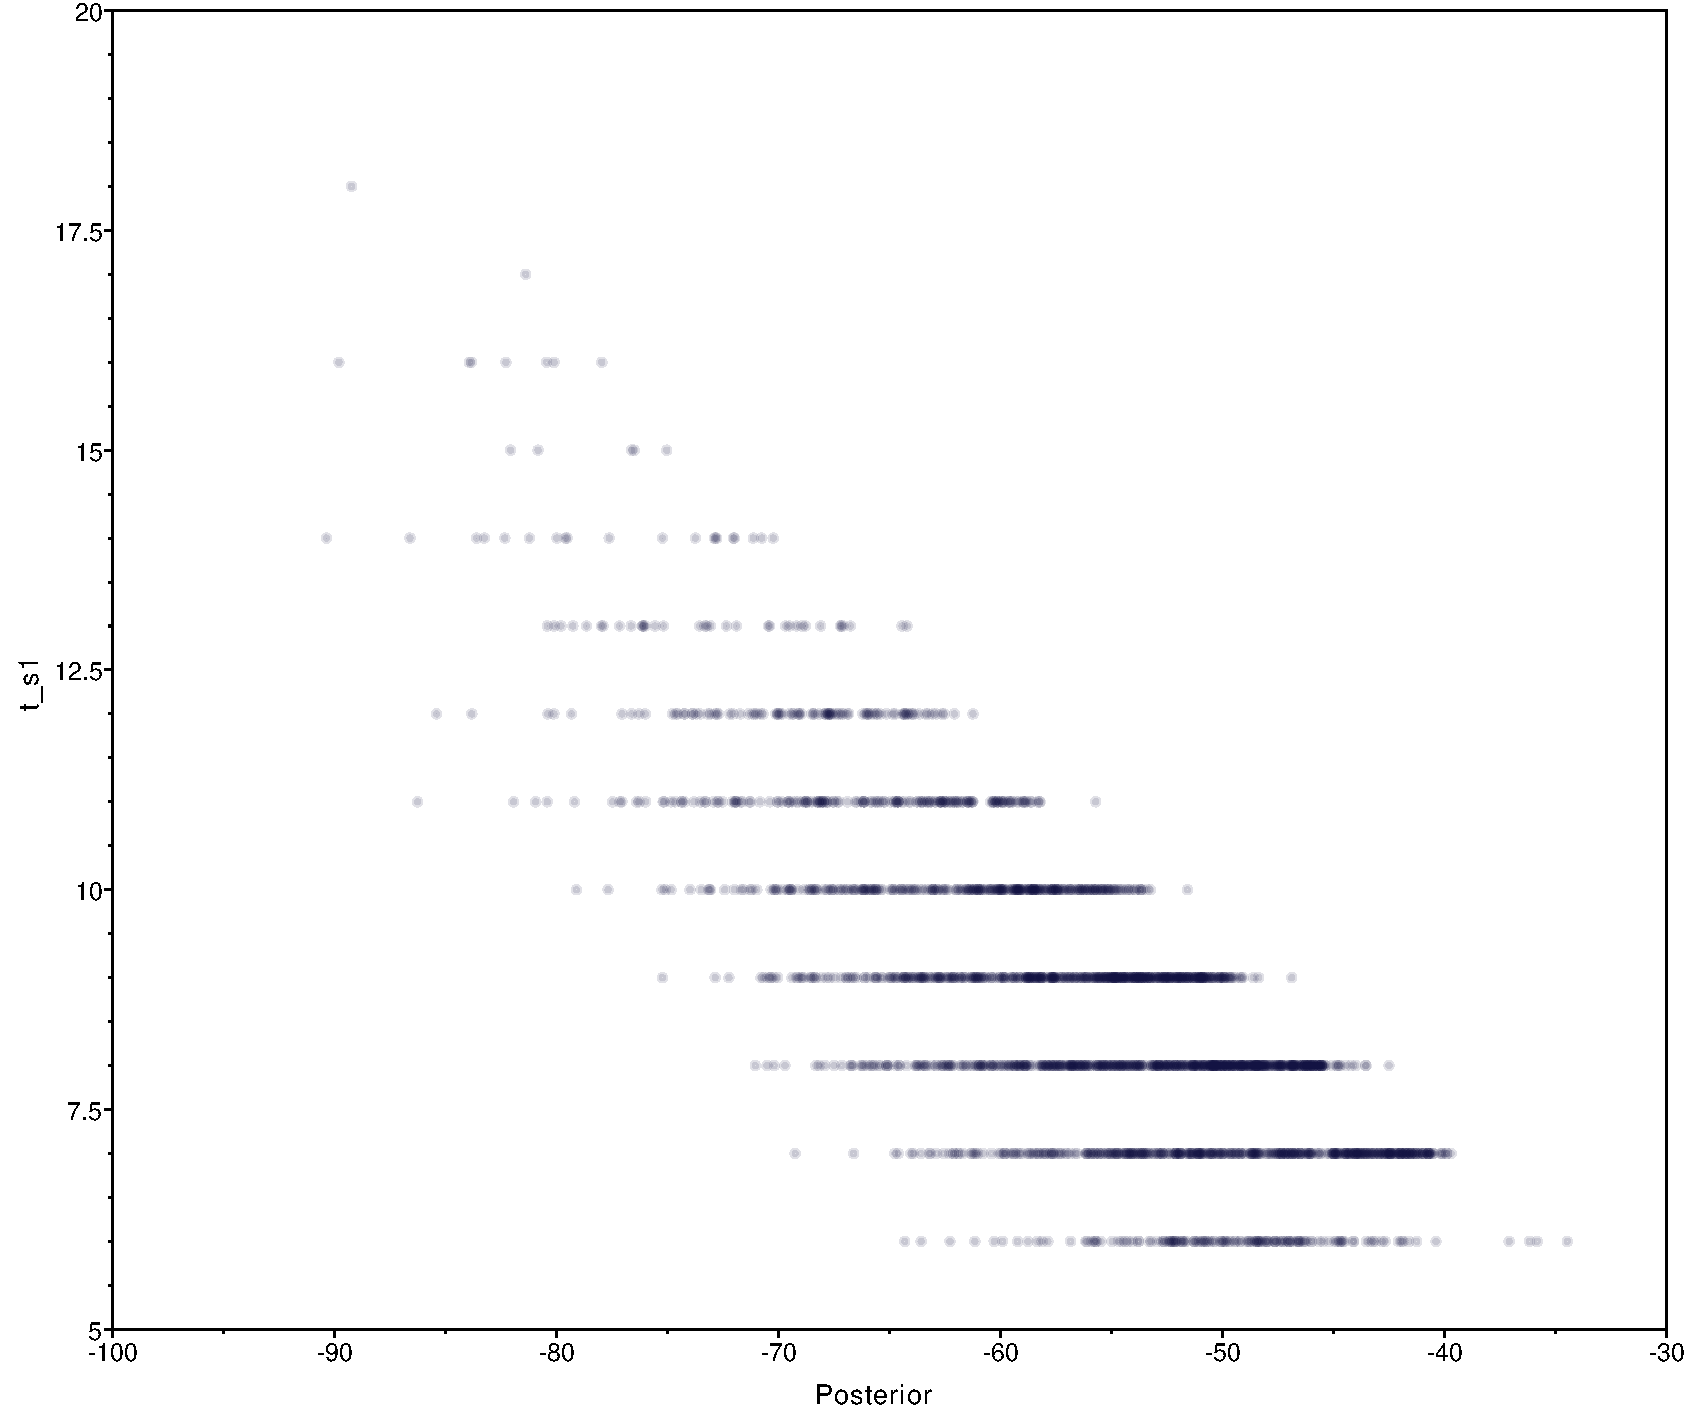
\includegraphics[width=3in]{RB_Biogeography_Tutorial/figures/joint_ngain_posterior}
\caption{Joint-marginal distribution of posterior and number dispersal events summed over the tree.}
\end{figure}

One interesting facet of this output is there are never fewer than six events.
In fact, since we assume a stratified geography and that only one event may occur per instant, it is impossible to describe the data we see at the tips with fewer than six gain events.
That is, six gain events is part of the maximum parsimony solution.

\subsection{Biogeographic event histories from {\tt mnCharHistoryNewick}}

For more detailed data exploration, this analysis also provides annotated Newick strings with the complete character mappings for the tree.

\noindent \\ \impmark Open {\tt ./output/bg\_2rate.events.txt} in a text editor.

\begin{framed}
%\begin{lstlisting}[basicstyle=\tiny \listingsfont, columns=texcl]
\begin{lstlisting}
Iteration  Posterior  Likelihood  Prior  Tree
Iteration	Posterior	Likelihood	Prior	Tree
0	-51.3307	-56.0288	4.69806	((((((((P_hawaiiensis_WaikamoiL1[&index=18;nd=0010;pa=0010;ev={}]:0.96 ...
10	-54.4257	-58.1568	3.7311	((((((((P_hawaiiensis_WaikamoiL1[&index=18;nd=0010;pa=0010;ev={}]:0.96 ...
20	-58.0696	-62.0923	4.02274	((((((((P_hawaiiensis_WaikamoiL1[&index=18;nd=0010;pa=0010;ev={}]:0.96 ...
30	-46.5049	-51.1197	4.6148	((((((((P_hawaiiensis_WaikamoiL1[&index=18;nd=0010;pa=0010;ev={}]:0.96 ...
40	-42.8697	-46.4870	3.61735	((((((((P_hawaiiensis_WaikamoiL1[&index=18;nd=0010;pa=0010;ev={}]:0.96 ...
50	-43.5319	-47.4659	3.93394	((((((((P_hawaiiensis_WaikamoiL1[&index=18;nd=0010;pa=0010;ev={}]:0.96 ...

...
\end{lstlisting}
\end{framed}

Each iteration records the data-augmented character history (stochastic mapping) using metadata labels, which, for an internal node, looks like

\begin{snugshade}
\begin{lstlisting}
[&index=23;nd=0110;pa=0010;ch0=0010;ch1=0110;cs=s;bn=16;ev={{t:0.2513,a:1.1195,s:1,i:1}}
\end{lstlisting}
\end{snugshade}

{\tt index=23} indicates this branch leads to the node indexed 23.
The branch began in the ancestral state {\tt pa=0100} and terminated in the state {\tt nd=0110}.
Since this node is not a tip node, it represents a speciation event, so the daughter ranges are also given, {\tt ch0=0010} and {\tt ch1=0110}.
The cladogenic state for this speciation event was subset sympatric, {\tt cs=s}, rather than sympatric (wide or narrow; {\tt w} or  {\tt n}) or allopatric ({\tt a}).
Anagenic dispersal and extinction events occurring along the lineage leading to node 19 are recorded in {\tt events}, where each event has a time (relative to the absolute branch length), absolute age, state (into), and character index ({\tt t}, {\tt a}, {\tt s}, {\tt i}, resp.).
For this posterior sample of the character history for the branch leading to node 22, the species range expanded into Oahu at age 1.1195.

To manipulate this data format, we'll use Python scripts. Below are a few examples of interesting posterior features.

\noindent \\ \impmark  Open a Python console and read in the events.

\begin{snugshade}
\begin{lstlisting}
> cd scripts
> python27

...

>>> from bg_parse import *
>>> dd=get_events(fn="../output/bg_2rate.events")
\end{lstlisting}
\end{snugshade}

By default, {\tt get\_events()} extracts a dictionary where each node index maps to a branch's character history as reported in {\tt ./input/bg\_2rate.events.txt}. 
Each branch is a dictionary whose keys are various parts of the MCMC state and whose values the MCMC samples.
\begin{snugshade}
\begin{lstlisting}
>>> dd[23].keys()
['ch1', 'iteration', 'bn', 'nd', 'ch0', 'prior', 'posterior', 'cs', 'ev', 'likelihood']
>>> dd[23]['posterior'][0:5]
[-48.6952, -60.1832, -53.2286, -57.5778, -53.4633]
\end{lstlisting}
\end{snugshade}

To get the $n=1$ highest-valued sample for a branch by its posterior value
\begin{snugshade}
\begin{lstlisting}
>>> get_best(dd[23],n=1,p='posterior')
{'prior': [4.48225], 'iteration': [14890], 'bn': [22], 'nd': [[0, 1, 1, 0]], 'ch0': [[0, 1, 1, 0]], 'ch1': [[0, 0, 1, 0]], 'posterior': [-34.7139], 'pa': [[0, 1, 0, 0]], 'cs': ['subset_sympatry'], 'ev': [[{'age': 1.5637, 'state': 1, 'idx': 2, 'time': 0.8611}]], 'likelihood': [-39.1962]}
\end{lstlisting}
\end{snugshade}

To get the probability that area $i$ and area $j$ are both part of the species range as the branch for node 23 terminates, just before the speciation event
\begin{snugshade}
\begin{lstlisting}
>>> get_area_pair(dd[23])
[[0.0816, 0.0188, 0.0628, 0.0000],
 [0.0188, 0.7081, 0.4390, 0.0000],
 [0.0628, 0.4390, 0.7141, 0.0000],
 [0.0000, 0.0000, 0.0000, 0.0000]]
\end{lstlisting}
\end{snugshade}
showing area 3 was occupied nearly with probability 0.71 and both areas 2 and 3 were occupied with probability 0.44.
Note, Hawaii was submerged until approximately 0.5 million years ago, and thus the probability of being in that area is 0.0.

If the range is size one during a speciation event, the cladogenic event state is always narrow sympatric, {\tt `narrow\_sympatry'}.
But given the opportunity for non-sympatric events, i.e. that the range is larger than size one, we can get the probability of cladogenic state using
For the probability for cladogenic event state given the range was larger than size one
\begin{snugshade}
\begin{lstlisting}
>>> get_clado_state(dd[23])
{'allopatry': 0.0224, 'subset_sympatry': 0.1463, 'widespread_sympatry': 0.3183, 'narrow_sympatry': 0.5130}
>>> get_clado_state(dd[23],minSize=2)
{'allopatry': 0.0460, 'subset_sympatry': 0.3005, 'widespread_sympatry': 0.6535, 'narrow_sympatry': 0.0000}
>>> get_clado_state(get_best(dd[23],n=100),minSize=2)
{'allopatry': 0.1290, 'subset_sympatry': 0.6774, 'widespread_sympatry': 0.1936, 'narrow_sympatry': 0.0000}
\end{lstlisting}
\end{snugshade}

Depending on your question, different aspects of the posterior cladogenic state will interest you.
Narrow sympatry is the favored ancestral state, but wide sympatry is favored for ranges of size $n>1$.
However, when we look at the 100 most probable samples, subset sympatry becomes most favored.

More script functions are found in {\tt ./scripts/bg\_parse.py}.

\subsection{New Hampshire extended format file (\texttt{./output/bg\_2rate.nhx})}

Because this data is very high-dimensional, we'll use an external data exploration tool to look at range evolution.

This file summarizes the input and output from a BayArea analysis using NEXUS format containing a New Hampshire eXtended (NHX) tree string.
NHX allows you to annotate nodes in a Newick string with meta-information, which BayArea uses to report the probabilities in the \texttt{my\_run.area\_probs.txt} file.
The \texttt{geo} block gives the geographical latitudes and longitudes for the areas in the order they are reported as probabilities.
Like the \texttt{my\_run.area\_probs.txt} file, this file is not written until the analysis is complete.
This annotation is used for the two visualization programs covered in the next section, Phylowood and BayArea-Fig.
The anatomy of the Phylowood and BayArea-Fig settings blocks will also be explained there.

\section{Visualization}

Here we'll explore two options for visualizing ancestral range reconstructions.
I'll walk you through some of the basic functionality, but feel free to play around as you like.

\subsection{Phylowood}

Phylowood generates interactive animations to explore biogeographic reconstructions.

\noindent \\ \impmark Open \texttt{http://mlandis.github.io/phylowood}.

\noindent \\ \impmark Drag and drop \texttt{./output/bg\_2rate.nhx.txt} into the text field.

\begin{figure}[H]
\centering
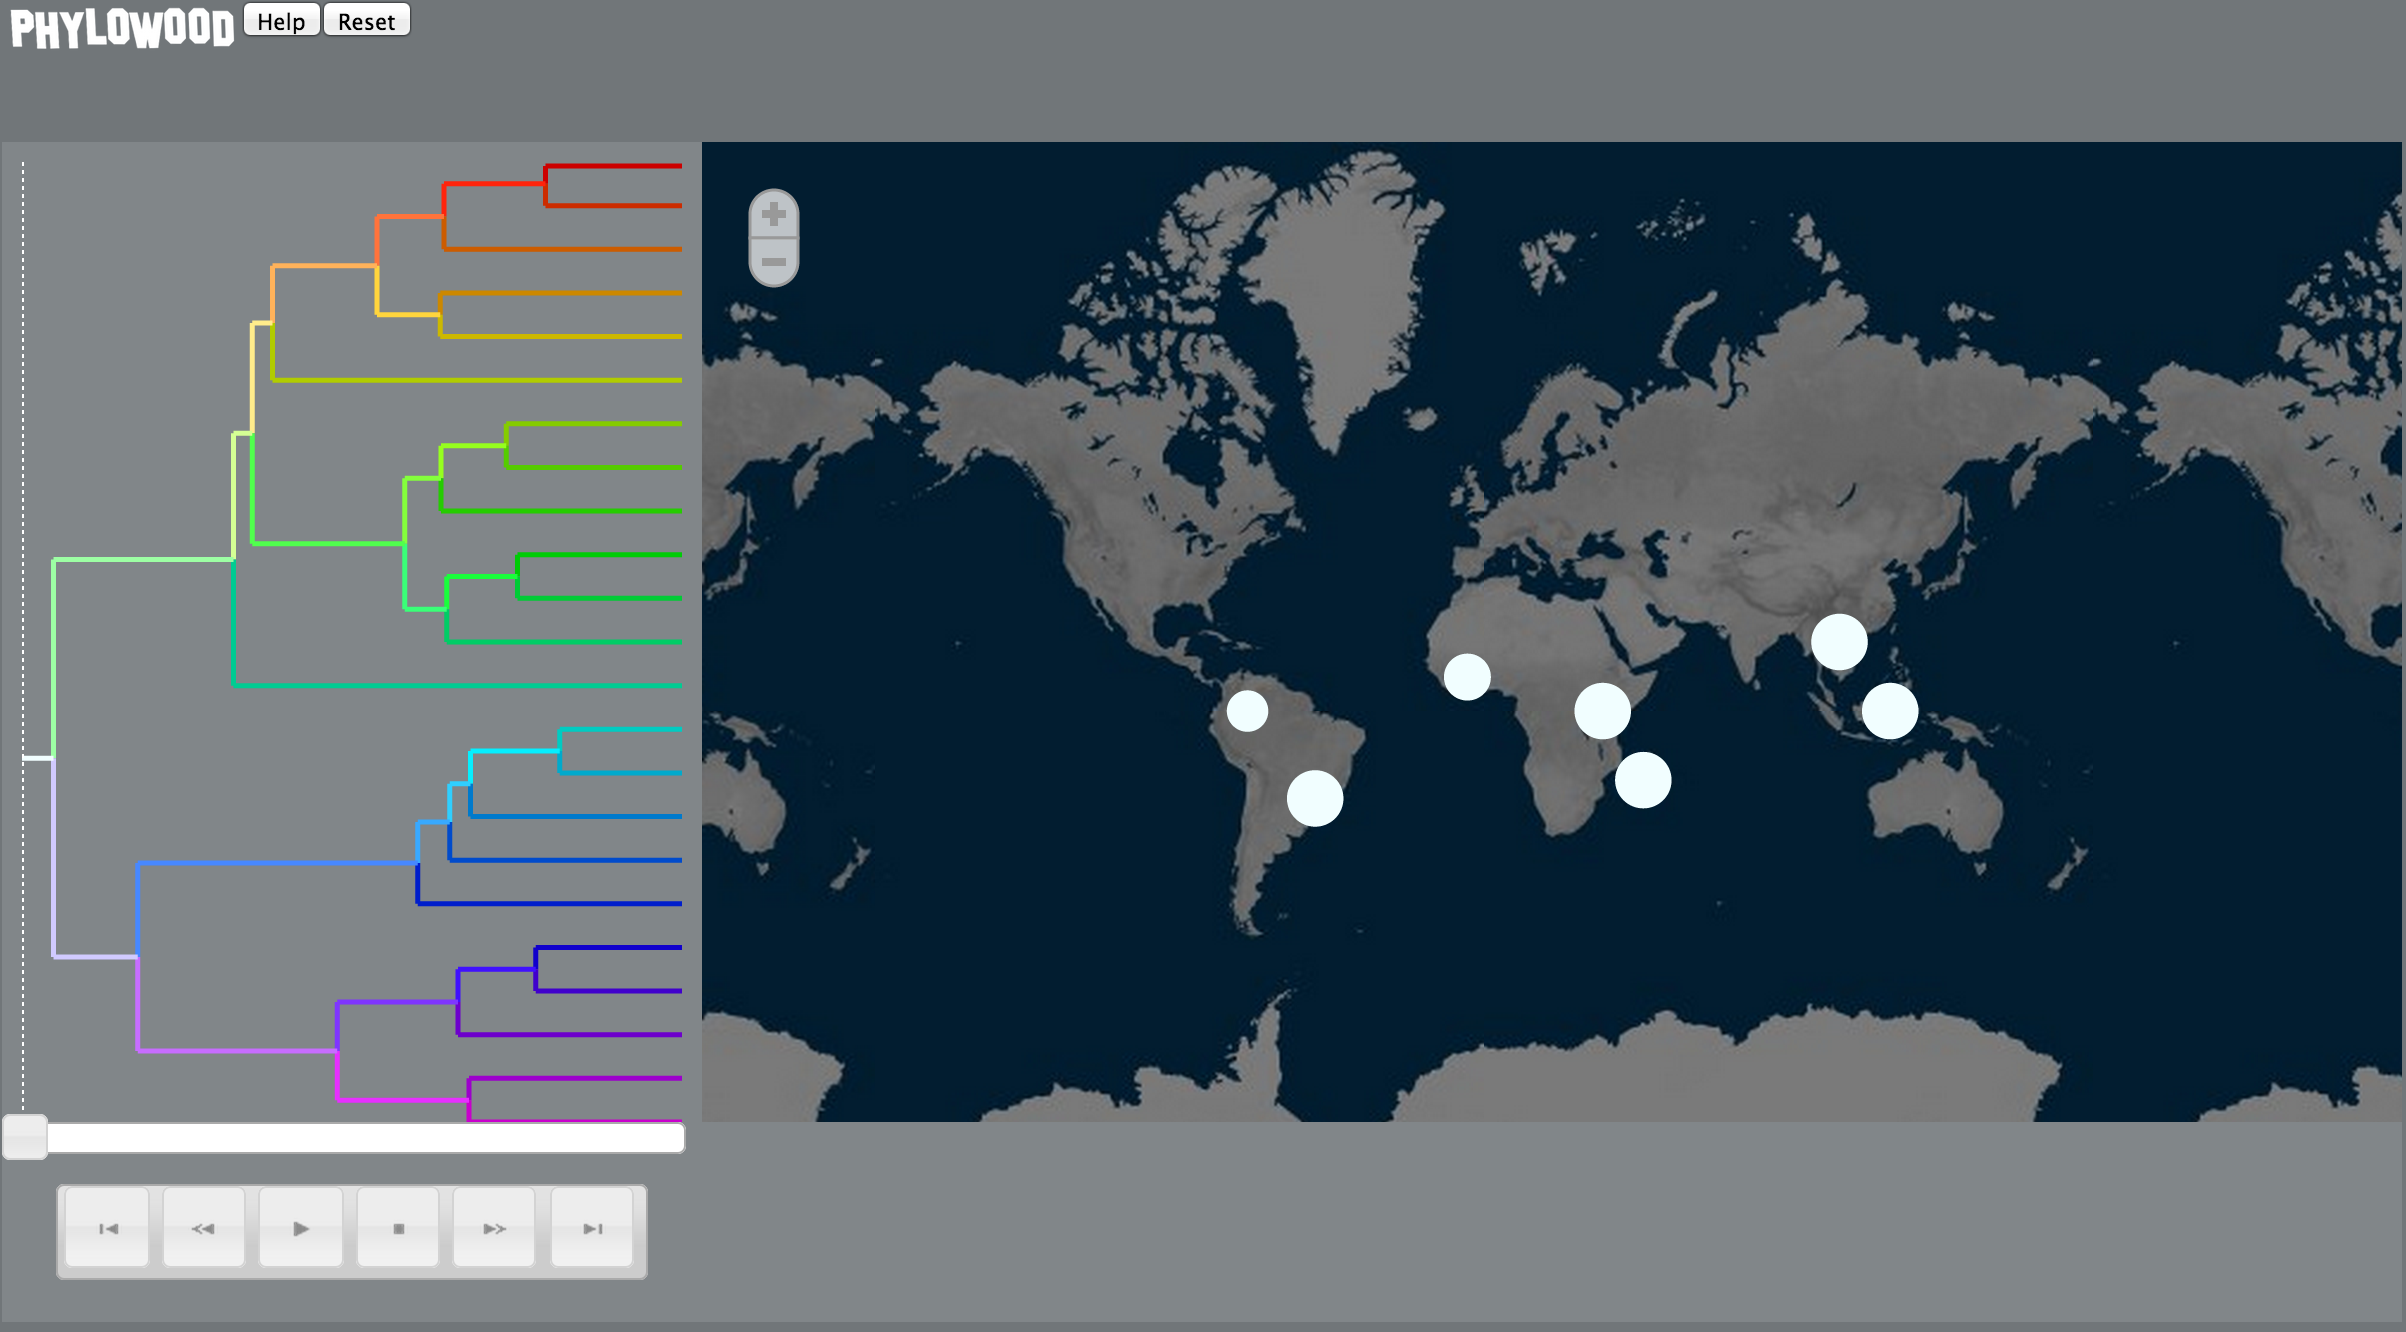
\includegraphics[width=4in]{RB_Biogeography_Tutorial/figures/phw_mrca}
\caption{Phylowood frame showing posterior ancestral range of root node.}
\end{figure}

\noindent \\ \impmark Click the Play button to view the animation. \\

There are three control panels to help you filter data: the media panel, the map panel, and the phylogeny panel.
The media buttons correspond to Beginning, Slow/Rewind, Play, Stop, Fast Forward, Ending (from left to right).
The animation will play the timeframe corresponding to the slider.

\noindent \\ \impmark Drag the slider to the right (the present).

\begin{figure}[H]
\centering
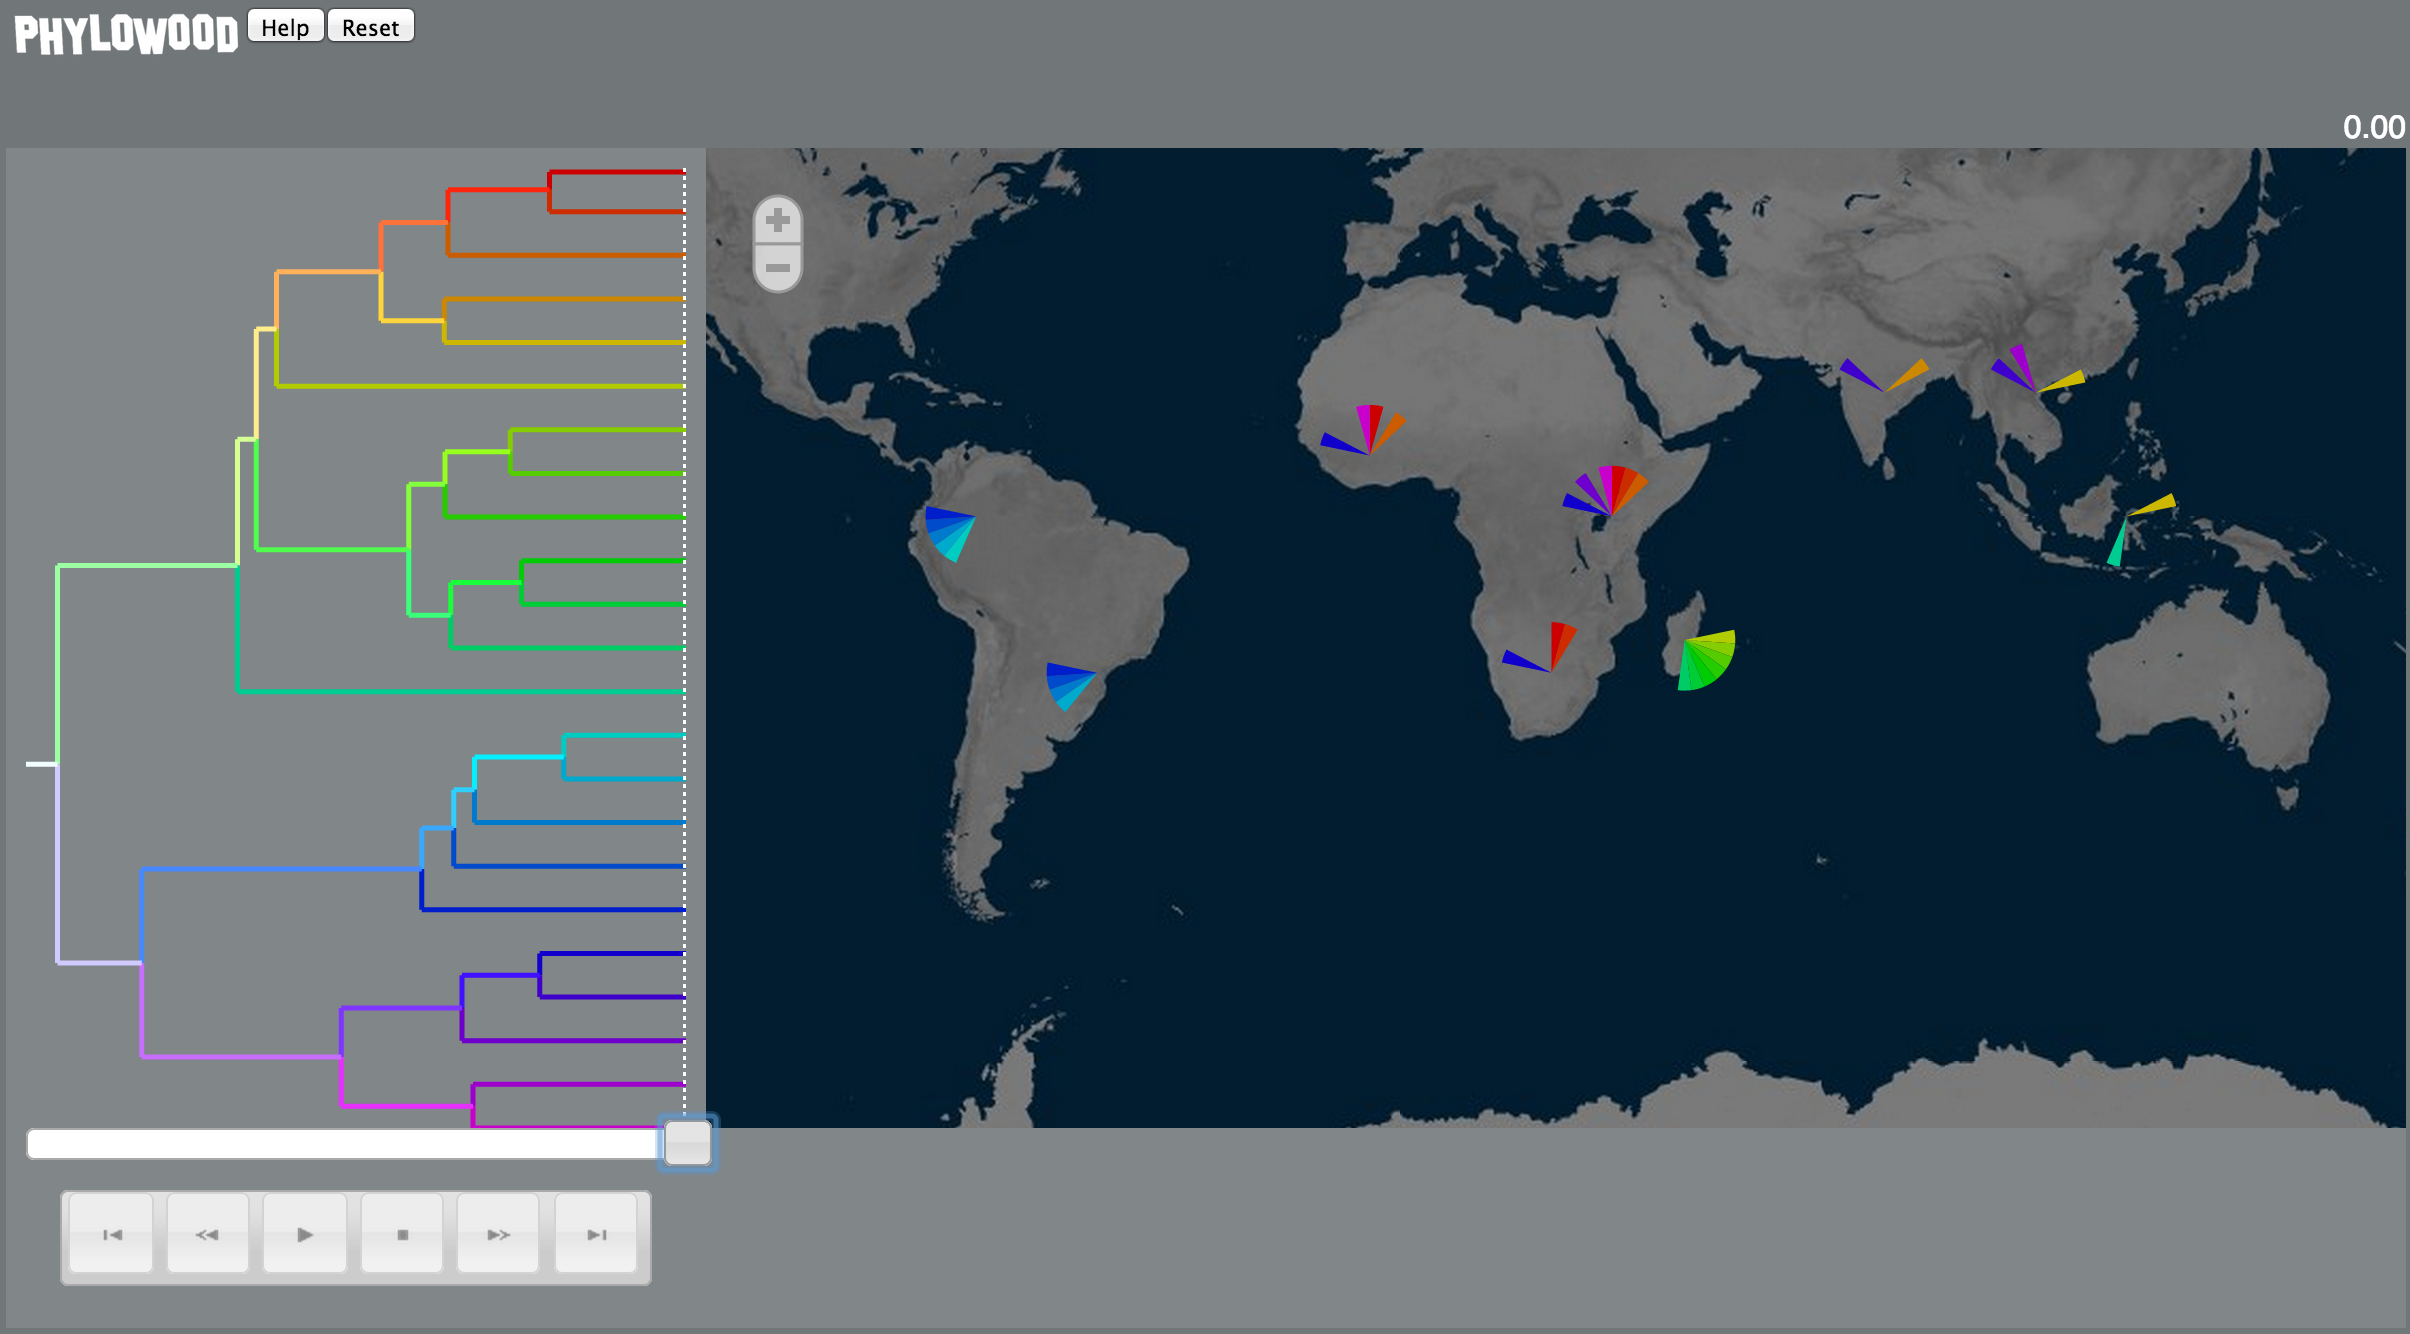
\includegraphics[width=4in]{RB_Biogeography_Tutorial/figures/phw_all}
\caption{Phylowood frame showing distribution of extant taxon ranges.}
\end{figure}

\noindent \\ \impmark Pan and zoom around the map.\\

Marker colors correspond to the phylogenetic lineages in the phylogeny panel.
Markers are split into slices and (loosely) sorted phylogenetically, so nearby slices are generally closely related.
At divergence events, a marker's radius is proportional to the marginal posterior probability the node was present in the area at that time.
Between divergence events, marker's radius is simply an interpolation of the values at the two endpoints.
Some information about geological constraints and cladogenic events is lost.

\noindent \\ \impmark Mouseover an area to learn which lineage it belongs to and its presence probability. \\

Since it's difficult to see how specific clades evolve with so many taxa, Phylowood offers two ways to filter taxa from the animation.
We call the set of a lineage, all its ancestral lineages towards the root, and all descendant lineages a phylogenetic heritage.
The root's heritage is the entire clade.
A leaf node's heritage is a path from the tip to the root.

\noindent \\ \impmark Mouseover a lineage to temporarily highlight the lineage's heritage. Remove the mouseover to remove the highlight effect. \\

The highlight effect is temporary and quickly allows you to single out lineages of interest during animation.
Phylowood also offers a masking effect that persists until an unmask command is issued.

\noindent \\ \impmark Double-click the white root branch to mask the root node's heritage (all lineages). Single click a lineage to unmask that lineage's heritage. \\

\begin{figure}[H]
\centering
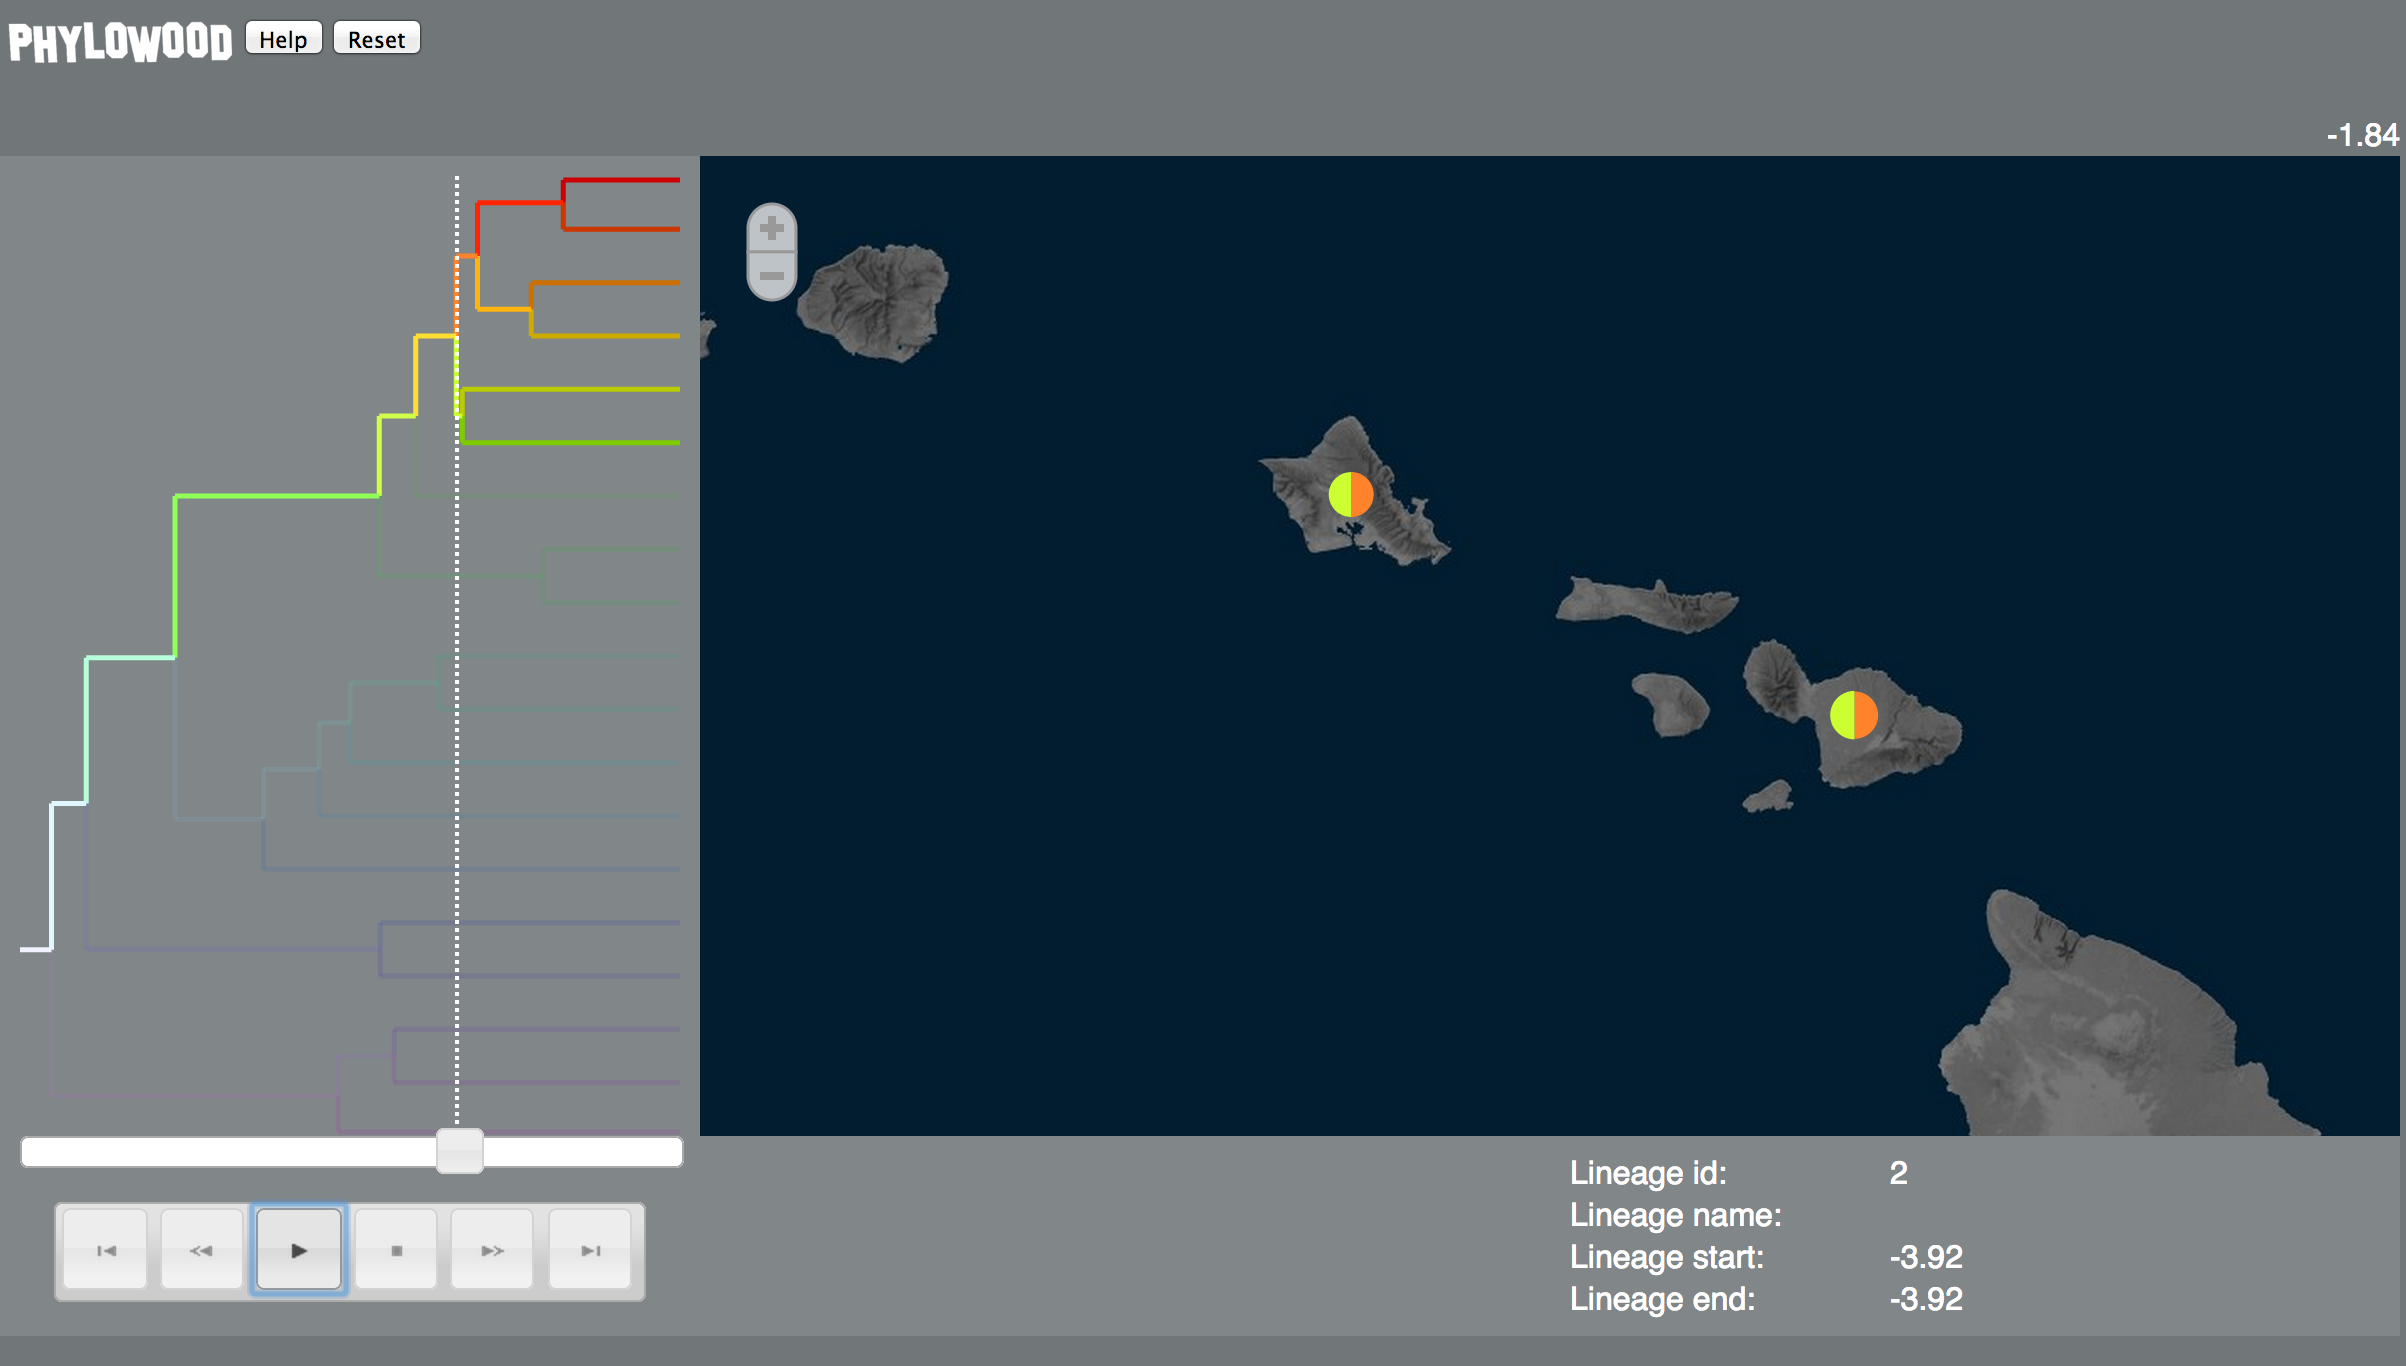
\includegraphics[width=4in]{RB_Biogeography_Tutorial/figures/phw_br23}
\caption{Phylowood frame highlighting the posterior range for the most recent common ancestor of {\it P. mauiensis} and {\it P. hawaiiensis}.}
\end{figure}

Now that the masking effects are in place, you're free to interact with other map components.
In addition, the area of marker sizes is only distributed among unmasked lineages.

\noindent \\ \impmark Visit \texttt{https://github.com/mlandis/phylowood/wiki} to learn more about Phylowood.

\bibliographystyle{mbe}
\bibliography{RB_Biogeography_Tutorial/bayes}




\part{Phylogenetic Comparative Method}
\chapter{Phylogenetic Comparative Analyses: Continuous Trait Evolution}
\section{Introduction}

The subject of the comparative method is the analysis of trait evolution at the macroevolutionary scale.
In a comparative context, many different questions can be addressed: tempo and mode of evolution, correlated evolution of multiple quantitative traits, trends and bursts, changes in evolutionary mode correlated with major key innovations in some groups, etc \citep[for a good introduction see][]{Harvey1991}.

In order to correctly formalize comparative questions, the underlying phylogeny should always be explicitly accounted for. This point is clearly illustrated, in particular, by the independent contrasts method \citep{Felsenstein1985,Huelsenbeck2003}. Practically speaking, the phylogeny and the divergence times are usually first estimated using a separate phylogenetic reconstruction software. In a second step, this time-calibrated phylogeny is used as an input to the comparative method.
Doing this, however, raises a certain number of methodological problems:
\begin{itemize}
\item
the uncertainty about the phylogeny (and about divergence times) is ignored
\item
the traits themselves may have something to say about the phylogeny
\item
the rate of substitution, and more generally the parameters of the substitution process, can also be seen as quantitative traits, amenable to a comparative analysis.
\end{itemize}
All these points are not easily formalized in the context of the step-wise approach mentioned above.
Instead, what all this suggests is that phylogenetic reconstruction, molecular dating and the comparative method should all be considered jointly, in the context of one single overarching probabilistic model.

Thanks to its modular structure, \RevBayes~represents a natural framework for attempting this integration.
The aim of the present tutorial is to guide you through a series of examples where this integration is achieved, step by step.
It can also be considered as an example of the more general perspective of \emph{integrative modeling}, which can be recruited in many other contexts.



%%%%%%%%
%%   Data   %%
%%%%%%%%
\section{Data and files}

We provide several data files which we will use in this tutorial.
You may want to use your own data instead.
In the \cl{data} folder, you will find the following files
\begin{itemize}
\item
\cl{primates\_cytb.nex}: Alignment of the \textit{cytochrome b} subunit from 23 primates representing 14 of the 16 families (\textit{Indriidae} and \textit{Callitrichidae} are missing).

\item
\cl{primates\_lhtlog.nex}: 2 life-history traits (endocranial volume (ECV), body mass; each for males and females separately)  for 23 primate species \citep[taken from the Anage database,][]{DeMagalhaes2009}. The traits have been log-transformed.

\item
\cl{primates.tree}: A time calibrated phylogeny of the same 23 primates.
\end{itemize}





\section{Univariate Brownian evolution of quantitative traits}

\label{univariate}

As a first preliminary exercise, we wish to reconstruct the evolution of body mass in primates and, in particular, estimate the body mass of their last common ancestor.
For this, we will assume that the logarithm of body mass follows a simple univariate Brownian motion along the phylogeny.
In a first step, we will ignore phylogenetic uncertainty:
thus, we will assume that the Brownian process describing body mass evolution runs along a fixed time-calibrated phylogeny (with fixed divergence times), such as specified in the file \cl{primates.tree}.

\noindent \\ \impmark You may want to take the time to visualize the tree given in \cl{primates.tree} as well as the matrix of quantitative traits specified by the \cl{primates\_lhtlog.nex} file, before going into the modeling work described below.


\subsection{The model and the priors}

A univariate Brownian motion $x(t)$ is parameterized by its starting value at the root of the phylogeny $x(0)$ and a rate parameter $\sigma$. This rate parameter tunes the amplitude of the variation per unit of time. Specifically, along a given time interval $(0,T)$, the value of $X$ at time $T$ is normally distributed, with mean $x(0)$ and variance $\sigma^2 T$:
\begin{eqnarray*}
x(T) & \sim & \text{Normal} \left( x(0), \sigma^2 T \right).
\end{eqnarray*}

Concerning $\sigma$, we can formalize the idea that we are ignorant about the \emph{scale} (the order of magnitude) of this parameter by using a log-uniform prior:
\begin{eqnarray*}
\sigma &\sim& \frac{1}{\sigma}.
\end{eqnarray*}

Concerning the initial value $x(0)$ of the Brownian process at the root of the phylogeny.
Alternatively, you may want to specify a normal distribution as the prior distribution on the root value if you have some prior information.

Finally, the tree topology $\psi$ is, as mentioned above, fixed to some externally given phylogeny.
The entire model is now specified: tree $\psi$, variance $\sigma$ and Brownian process $x(t)$:
\begin{eqnarray*}
\sigma &\sim& \frac{1}{\sigma},
\\
x(0) &\sim& \text{Uniform},
\\
x(t) \mid \Psi, \sigma &\sim& \text{Brownian} \left( x(0), \, \psi, \, \sigma \right).
\end{eqnarray*}
Conditioning the model on empirical data by clamping $x(t)$ at the tips of the phylogeny, we can then run a MCMC to sample from the joint posterior distribution on $\sigma$ and $x$. Once this is done, we can obtain posterior means, medians or credible intervals for the value of body mass or other life-history traits for specific ancestors.


\subsection{Programming the model in \RevBayes}

The problem of continuous trait evolution ---just as for discrete trait evolution--- along a phylogeny is that we do not know the values of the traits at the internal nodes. That means, that we need to treat the states at the internal nodes as additional parameters of the model. For discrete characters we use the sum-product (a.k.a.~pruning) algorithm \citep{Felsenstein1981} to analytically integrate over all possible states at the internal nodes. For continuous characters (traits) similar methods have been proposed.
In \RevBayes~you have three main ways of specifying this model and running an analysis on it. The three approaches are: (1) phylogenetic independent contrasts using the reduced likelihood (REML), (2) Brownian motion using a phylogenetic covariance matrix, and (3) a full Brownian motion model using data augmentation.
Each of these approaches has there advantages and disadvantages as will be explained below.
Nevertheless, all approaches give the same results in terms of rate estimation.


\subsection{Phylogenetic Independent Contrasts using the reduced likelihood (REML)}

The reduced or restricted maximum likelihood (REML) method computes the probability of observing the continuous character at the tips by an analytical solution to integrate over the internal states \citep{Felsenstein1985}. 
This analytical solution is very fast to compute and thus can be applied to large phylogenies and/or many independent characters. However, the REML method looses the information about the location of the root state and thus you cannot infer which state the root or other internal nodes have.

You do not need to understand the algorithm but we provide a sketch of the idea behind REML to give you some insights.
REML compute the values at the internal nodes as the phylogenetic contrasts $x_k = x_i - x_j$ where $x_i$ and $x_j$ are the values of the child nodes in the phylogeny.
Then, we can compute the probability of observing the contrast $x_k$ using the probability density of a normal distribution with mean $\mu = 0$ and standard deviation $\sigma = \sqrt{\nu_i + \delta_i + \nu_j + \delta_j}$ where $\nu_i$ and $\nu_j$ are the (scaled) branch lengths leading to node $i$ and $j$ respectively. $\delta$ is the additional uncertainty that is propagated through the phylogeny  and is compute by $\delta_k = ((\nu_i + \delta_i)*(\nu_j + \delta_j)) / (\nu_i + \delta_i + \nu_j + \delta_j)$. These computations are done for you in the \RevBayes~distribution called \cl{dnPhyloBrownianREML}.

In the directory \cl{RevBayes\_scripts/} you will find a script called \cl{primatesMass\_BM\_REML.Rev}.
This script implements the univariate Brownian model described above. Instead of re-typing the content of script entirely in the context of an interactive \RevBayes~session, you can instead run the script directly:
{\tt \small \begin{snugshade*}
\begin{lstlisting}
source("RevBayes\_scripts/primatesMass_BM_REML.Rev")
\end{lstlisting}
\end{snugshade*}}
This script essentially reformulates what has been explained in the last subsection and serves as an example solution for you. For the later section you need to adjust the script.

Let us go through the script step by step in the \Rev~language.
First, load the trait data:
{\tt \small \begin{snugshade*}
\begin{lstlisting}
contData <- readContinuousCharacterData("data/primates_lhtlog.nex")
\end{lstlisting}
\end{snugshade*}}
If you type you will see that the continuous character data matrix contains several characters (columns). 
{\tt \small \begin{snugshade*}
\begin{lstlisting}
contData
|*
|*   Continuous character matrix with 23 taxa and 11 characters
|*   ==========================================================
|*   Origination:                   primates_lhtlog.nex
|*   Number of taxa:                23
|*   Number of included taxa:       23
|*   Number of characters:          11
|*   Number of included characters: 11
|*   Datatype:                      Continuous
\end{lstlisting}
\end{snugshade*}}
Since we only want the body mass (of females) we exclude all but the third character
{\tt \small \begin{snugshade*}
\begin{lstlisting}
contData.excludeAll()
contData.includeCharacter(3) 
\end{lstlisting}
\end{snugshade*}}

Next, load the time-tree from file. Remember that we use in this first simple example a fixed tree that we assume is known without uncertainty.
{\tt \small \begin{snugshade*}
\begin{lstlisting}
treeArray <- readTrees("data/primates.tree")
psi <- treeArray[1]
\end{lstlisting}
\end{snugshade*}}
\noindent \\ \impmark You may want to look at this tree before by loading the \cl{primates.tree} in FigTree or any other tree visualization software.

%Next we will specify some useful variables based on our dataset. The variable \cl{data} has \textit{member functions} that we can use to retrieve information about the dataset. 
%These include the number of species (\cl{n\_species}), the tip labels (\cl{names}), and the number of internal branches (\cl{n\_branches}).
%Each of these variables will be necessary for setting up different parts of our model.
%{\tt \begin{snugshade*}
%\begin{lstlisting}
%n_species <- data.ntaxa()
%names <- data.names()	
%n_branches <- 2 * n_species - 3 
%\end{lstlisting}
%\end{snugshade*}}

As usual, we start be initializing some useful helper variables.
For example, we set up a counter variable for the number of moves that we already added to our analysis.
This will make it much easier if we extend the model or analysis to include additional moves or to remove some moves.
{\tt \begin{snugshade*}
\begin{lstlisting}
mi = 0 
\end{lstlisting}
\end{snugshade*}}

Then, we define the overall rate parameter $\sigma$ which we assign a (truncated) log-uniform prior. Note that it is more efficient in Bayesian inference to specify a uniform prior and then to transform the parameter which we will use here:
{\tt \small \begin{snugshade*}
\begin{lstlisting}
logSigma ~ dnUniform(-5,5)
sigma := 10^logSigma
\end{lstlisting}
\end{snugshade*}}
Using this approach we have specified a prior probability distribution on \cl{sigma} between $10^{-5}$ to $10^5$ which should be broad enough to include all reasonable values.
%To accelerate convergence, it can be useful to force initialization of $\sigma$ to a small value:
%{\tt \small \begin{snugshade*}
%\begin{lstlisting}
%sigma.setValue(0.1)
%\end{lstlisting}
%\end{snugshade*}}

Since the rate of trait evolution \cl{logSigma} is a stochastic variable and we want to estimate it, we need to add a sliding move on it. Remember that the sliding move proposes new values drawn from a window with width \cl{delta} and is centered around the current values; thus it slides through the parameter space together with the current parameter value.
{\tt \small \begin{snugshade*}
\begin{lstlisting}
moves[++mi] = mvSlide(logSigma, delta=1.0, tune=true, weight=2.0)
\end{lstlisting}
\end{snugshade*}}

Next, define a random variable from the univariate Brownian-Phylo-REML process, which we will call \cl{logmass}.
We need to provide the tree variable \cl{psi}, some branch-specific rate multiplier parameter which we simply set to 1, the shared rate for this site \cl{sigma} and the number of sites (number of continuous traits) that we use. 
{\tt \small \begin{snugshade*}
\begin{lstlisting}
logmass ~ dnPhyloBrownianREML(psi, branchRates=1.0, siteRates=sigma, nSites=1)
\end{lstlisting}
\end{snugshade*}}
Now, condition the Brownian model on empirically observed values for body mass in the extant taxa.
{\tt \small \begin{snugshade*}
\begin{lstlisting}
logmass.clamp( contData )
\end{lstlisting}
\end{snugshade*}}

The model is now entirely specified and we can create a model object containing the entire model graph by providing it with only one of our model variables, \EG \cl{sigma}. 
{\tt \small \begin{snugshade*}
\begin{lstlisting}
mymodel = model(sigma)
\end{lstlisting}
\end{snugshade*}}

To see what it happing during the MCMC let us make a screen monitor that tracks the rate \cl{sigma}.
{\tt \small \begin{snugshade*}
\begin{lstlisting}
monitors[1] = mnScreen(printgen=10, sigma)
\end{lstlisting}
\end{snugshade*}}

Additionally, we'll use a file monitor that does the same thing, but directly stores the values into a file.
{\tt \small \begin{snugshade*}
\begin{lstlisting}
monitors[2] = mnFile(filename="output/primates_mass_REML.log", printgen=10, separator = TAB, sigma)
\end{lstlisting}
\end{snugshade*}}

We can finally create a mcmc, and run it for a good 100 000 cycles after we did a burnin phase of 10 000 iterations:
{\tt \small \begin{snugshade*}
\begin{lstlisting}
mymcmc = mcmc(mymodel, monitors, moves)
mymcmc.burnin(generations=10000,tuningInterval=500)
mymcmc.run(100000)
\end{lstlisting}
\end{snugshade*}}




\subsection*{Exercises}

\begin{itemize}
\item
Run the model.
\item
using \cl{Tracer}, visualize the posterior distribution on the rate parameter \cl{sigma}
\item
calculate the 95\% credible interval for the rate of evolution of the log of body mass ($\sigma$)
\end{itemize}


\vspace{5cm}






\subsection{Phylogenetic covariance matrix}

The second method that we will use creates a phylogenetic covariance matrix. The phylogenetic covariance matrix method integrates over the states  at the internal nodes as well but uses instead a multivariate normal distribution.
The key advantage is that this method provides information about the root state since it models the root state as an additional parameter of the model. The disadvantage is that it is very computationally intensive. That means, that the phylogenetic covariance matrix approach may take long for very large data sets (at least in its current implementation).

\noindent \\ \impmark Copy the file \cl{primatesMass\_BM\_REML.Rev}, name it for example \cl{primatesMass\_BM\_Cov.Rev} and start editing it.

In the previous example, the REML approach, we did not specify a parameter for the state at the root.
In this exercise, we need this additional parameter.
Let us use a uniform prior distribution on the logarithm of the root mass.
A uniform prior between -100 and 100 should be diffuse enough. Just image how big or small an individual needs to be if it has body mass smaller than exp(-100) or larger than exp(100).
{\tt \small \begin{snugshade*}
\begin{lstlisting}
rootlogmass ~ dnUniform(-100,100)
\end{lstlisting}
\end{snugshade*}}
Next, we'll specify a sliding move that proposes new values for the \cl{rootlogmass} randomly drawn from a window centered around the current value.
{\tt \small \begin{snugshade*}
\begin{lstlisting}
moves[++mi] = mvSlide(rootlogmass,delta=10,tune=true,weight=2) 
\end{lstlisting}
\end{snugshade*}}

Finally, we need to substitute the \cl{dnPhyloBrownianREML} by \cl{dnPhyloBrownianMVN} to use the phylogenetic covariance matrix approach.
Again, we provide the tree variable \cl{psi}, some branch-specific rate multiplier parameter which we simply set to 1, the shared rate for this site \cl{sigma} and the number of sites (number of continuous traits) that we use. 
{\tt \small \begin{snugshade*}
\begin{lstlisting}
logmass ~ dnPhyloBrownianMVN(psi, branchRates=1.0, siteRates=sigma, rootStates=rootlogmass, nSites=1)
\end{lstlisting}
\end{snugshade*}}
This will automatically connect the parameters of the model together.

Additionally, we now have the extra parameter \cl{rootlogmass} which we want to monitor.
Thus we need to replace the file monitor and use instead.
{\tt \small \begin{snugshade*}
\begin{lstlisting}
monitors[2] = mnFile(filename="output/primates_mass_Cov.log", printgen=10, separator = TAB, sigma, rootlogmass)
\end{lstlisting}
\end{snugshade*}}


\noindent \\ \impmark Don't forget to change the output file names in the monitors, otherwise your old analyses files will be overwritten.


\subsection*{Exercises}

\begin{itemize}
\item
Run the analysis.
\item
Using \cl{Tracer}, visualize the posterior distribution on the rate parameter \cl{sigma} and the \cl{rootlogmass}
\item 
How does the posterior distribution of \cl{sigma} looks compared with the first analysis?
\item
Calculate the 95\% credible interval for the rate of evolution of the log of body mass ($\sigma$) and the \cl{rootlogmass}
\end{itemize}

\vspace{5cm}








\subsection{Data augmentation}

The third method to we will use is a data augmentation method. The data augmentation method uses explicitly the states at the internal nodes. We will specify the full model in \Rev.
That means that we will create a random variable for each node of the tree using a for loop. Each trait is then simply assign a normal distribution, as we described above in the model description.
The advantage of this method is that you estimate the values at the internal nodes directly and that you have full control about modifying any part of the model. The disadvantage is that the MCMC algorithm will be harder if you want to jointly estimate the phylogeny, although the likelihood computation is very fast. The problem is the mixing of the MCMC because proposing new trees involves proposing new good values for the states at the internal nodes.

\noindent \\ \impmark Copy the file \cl{primatesMass\_BM\_REML.Rev}, name it for example \cl{primatesMass\_BM\_DA.Rev} and start editing it.

]As in the previous example we will use a uniform prior distribution on the logarithm of the root mass.
{\tt \small \begin{snugshade*}
\begin{lstlisting}
rootlogmass ~ dnUniform(-100,100)
\end{lstlisting}
\end{snugshade*}}
Again, we'll specify a sliding move that proposes new values for the \cl{rootlogmass} randomly drawn from a window centered around the current value.
{\tt \small \begin{snugshade*}
\begin{lstlisting}
moves[++mi] = mvSlide(rootlogmass,delta=10,tune=true,weight=2) 
\end{lstlisting}
\end{snugshade*}}

In order to create the random variables for the internal states we need to know the number of nodes and the number of tips.
We will store these as some helper variables.
{\tt \small \begin{snugshade*}
\begin{lstlisting}
numNodes = psi.nnodes()
numTips = psi.ntips()
\end{lstlisting}
\end{snugshade*}}

Now we are ready to specify the Brownian motion model for each branch.
That is, we simply specify a new normal distributed random variable for each node with mean being equal to the value of the parent variable and the standard deviation being equal to the product of the square root of the branch length and our rate parameter \cl{sigma}. We store all the variables in the vector \cl{logmass}. Then we are able to access the value at the parent node using the index of the parent node, which we can obtain from the tree using the function \cl{psi.parent(i)}. Similarly, since the variance depends on the branch length we retrieve the branch length of node with index \cl{i} using the function \cl{psi.branchLength(i)}.

First we need to copy (create a reference to) the \cl{rootlogmass}
{\tt \small \begin{snugshade*}
\begin{lstlisting}
logmass[numNodes] := rootlogmass
\end{lstlisting}
\end{snugshade*}}
Let us start by creating the random variables for the internal nodes. Remember that the variance is equal to \cl{sigma}-squared times the branch length, and we need to compute the square root of it to obtain the standard deviation.
{\tt \small \begin{snugshade*}
\begin{lstlisting}
# univariate Brownian process along the tree
# parameterized by sigma
for (i in (numNodes-1):(numTips+1) ) {
  logmass[i] ~ dnNormal( logmass[psi.parent(i)], sd=sigma*sqrt(psi.branchLength(i)) )
  # moves on the Brownian process
  moves[++mi] = mvSlide( logmass[i], delta=10, tune=true ,weight=2) 
}
\end{lstlisting}
\end{snugshade*}}
You may have noticed that we specified in the loop a move for each internal \cl{logmass}. This is because we want to use the MCMC algorithm to integrate over the uncertainty in the states.

Next, we repeat the same loop but now for the tip nodes. Instead of applying a move to each tip node we will clamp the nodes. The nodes will be clamped with the data that we read in before.
{\tt \small \begin{snugshade*}
\begin{lstlisting}
for (i in numTips:1 ) {
  logmass[i] ~ dnNormal( logmass[psi.parent(i)], sd=sigma*sqrt(psi.branchLength(i)) )

  # condition Brownian model on quantitative trait data (second column of the dataset)
  logmass[i].clamp(contData.getTaxon(psi.nodeName(i))[1])
}
\end{lstlisting}
\end{snugshade*}}
Here we do not need a \cl{dnPhyloBrownianREML} or \cl{dnPhyloBrownianMVN} distribution anymore because we explicitly instantiated the model. Note that the approach we have taken using the loop is the tree-plate approach described in \citep{Hohna2014b}

Since we have several additional parameters ---the states at the internal nodes--- we will use a model monitor to write to file instead.
{\tt \small \begin{snugshade*}
\begin{lstlisting}
monitors[2] = mnModel(filename="output/primates_mass_DA.log", printgen=10, separator = TAB)
\end{lstlisting}
\end{snugshade*}}


\noindent \\ \impmark Don't forget to change the output file names in the monitors, otherwise your old analyses files will be overwritten.


\subsection*{Exercises}

\begin{itemize}
\item
Run the analysis.
\item
Using \cl{Tracer}, visualize the posterior distribution on the rate parameter \cl{sigma} and the \cl{rootlogmass} and the internal states.
\item 
How does the posterior distribution of \cl{sigma} looks compared with the first and second analysis?
\item
Calculate the 95\% credible interval for the rate of evolution of the log of body mass ($\sigma$) and the \cl{rootlogmass}. Have they changed?
\end{itemize}

\vspace{5cm}



\subsection{Brief intermediate summary}
In the above exercises you have analyzed the log-transformed body mass using a Brownian motion (BM) along a phylogeny. We assumed the phylogeny to be known without error and were primarily interested in the rate how fast the body mass evolves. The exercises showed you three different ways how to approach the BM model, each having its advantages and disadvantages. You will need to decide for your analysis which approach is most appropriate. Our intention was mainly to show you some of the flexibility in \RevBayes~how to specify the same model in many different ways, exposing sometimes more and sometimes less of the internal model graph structure. As an extra exercise you could start thinking about how to extend the basic BM.



\vspace{5cm}


\section{Multiple independently evolving traits}
The Brownian motion can easily be applied to multiple traits. The exactly same procedure and model will be applied as above and thus we will skip the repetitive description. The interesting questions that you can ask about multiple traits is ---amongst others--- if rates between traits vary.


As an example we use now the first four characters of the data matrix, which are: 1) female log endocranial volume (ECV), 2) male log ECV, 3) female log body mass and 4) male log body mass.
{\tt \small \begin{snugshade*}
\begin{lstlisting}
contData <- readContinuousCharacterData("data/primates_lhtlog.nex")
contData.excludeCharacter(5:11)
\end{lstlisting}
\end{snugshade*}}
In the first simple example we assume that all site rates are equal, thus we use a rate multiplier we we call \cl{perSiteRates}.
{\tt \small \begin{snugshade*}
\begin{lstlisting}
perSiteRates <- [1,1,1,1]
\end{lstlisting}
\end{snugshade*}}
Furthermore, we have now four characters and hence we will estimate a root state for each one of them. We use the same prior probability for every character, just as above for the single character example.
{\tt \small \begin{snugshade*}
\begin{lstlisting}
for (i in 1:4) {
   rootlogmass[i] ~ dnUniform(-100,100)
   moves[++mi] = mvSlide(rootlogmass[i],delta=10,tune=true,weight=2) 
}
\end{lstlisting}
\end{snugshade*}}

Finally, we bring together all the parameter to specify our Brownian motion model along the tree. Note that we specify here the site rates as the product of the global rate \cl{sigma} time the sites specific rates (which are, however all equal in this first exercie).
{\tt \small \begin{snugshade*}
\begin{lstlisting}
logmass ~ dnPhyloBrownianMVN(psi, branchRates=1.0, siteRates=sigma*perSiteRates, rootStates=rootlogmass, nSites=4)
\end{lstlisting}
\end{snugshade*}}

After this you need to create the model using the \cl{model} function, create your monitors, create the MCMC and finaly run the MCMC.


\subsection*{Exercises}

\begin{itemize}
\item
Run the analysis.
\item
Using \cl{Tracer}, visualize the posterior distribution on the rate parameter \cl{sigma} and the four \cl{rootlogmass} values.
\item 
Compare the results to the previous single trait analyses?
\end{itemize}

\vspace{5cm}



\subsection{Independent site rates}

{\tt \small \begin{snugshade*}
\begin{lstlisting}
perSiteRates ~ dnDirichlet([1,1,1,1])
moves[++mi] = mvSimplexElementScale(perSiteRates,alpha=10,tune=true,weight=4)
\end{lstlisting}
\end{snugshade*}}


\subsection*{Exercises}

\begin{itemize}
\item
Run the analysis.
\item
Using \cl{Tracer}, visualize the posterior distribution on the per site rate parameter \cl{perSiteRates}.
\item 
How are the estimate per site rates compared to each other?
\end{itemize}

\vspace{5cm}


\subsection{Partially shared site rates}
We hope that your results in the previous analysis showed that the rates for females and males for both the ECV and the body mass are very similar.
This motivates us to specify an explicit model where the rates between ECV and body mass evolution are different but shared between females and males.
We will model the difference using the \cl{siteRateDiff} parameter which is drawn from a Beta(1,1) distribution, which is essentially a uniform distribution between 0 and 1.
We still choose the Beta distribution because it is easier to specify more informative priors.
{\tt \small \begin{snugshade*}
\begin{lstlisting}
siteRateDiff ~ dnBeta(1,1)
\end{lstlisting}
\end{snugshade*}}
Next, we specify a sliding move on the \cl{siteRateDiff}.
{\tt \small \begin{snugshade*}
\begin{lstlisting}
moves[++mi] = mvSlide(siteRateDiff,delta=10,tune=true,weight=2)
\end{lstlisting}
\end{snugshade*}}
To obtain the rates we use \cl{siteRateDiff} as the rate for the ECV evolution in females and males and 1-\cl{siteRateDiff} as the rate for the body mass evolution in females and males.
Note, however, that we need a small workaround here. \Rev~is a strictly typed language, which you may have noticed. The per site rates need to be positive real number (negative rates obviously don't make sense). However, the difference between two number is not guaranteed to be positive, only if we know that the first term is larger than the second. This is exactly the case for 1-\cl{siteRateDiff} but \RevBayes~doesn't know this so we need to tell it by using the absolute value \cl{abs} function.
{\tt \small \begin{snugshade*}
\begin{lstlisting}
perSiteRates[1] := siteRateDiff
perSiteRates[2] := siteRateDiff
perSiteRates[3] := abs(1.0 - siteRateDiff)   # specify the type here
perSiteRates[4] := abs(1.0 - siteRateDiff)
\end{lstlisting}
\end{snugshade*}}
You could have specified many other prior distribution on the relative rate (or ratio) such as a uniform prior distribution and then use logit or hyperbolic tangent transformation.
The only important factor is that the rates are somehow normalized because we use the global, shared rate \cl{sigma}.
Using the beta distribution makes the rates automatically normalized because the two different rates sum to one. Note that in the previous all four rates summed to 1.0 and here the two different rates sum to 1.0. This has the effect that we should estimate the global rate \cl{sigma} to be half of what you estimated previously. You may want to check this once you ran the analysis and loaded the output into \Tracer. 


The remaining functions are the same as in the previous example.


\subsection*{Exercises}

\begin{itemize}
\item
Run the analysis.
\item
Using \cl{Tracer}, visualize the posterior distribution on the per site rate parameter \cl{perSiteRates}.
\item 
Does the value of equal rate (\cl{siteRateDiff}=0.5) fall into the 95\% credible interval?
\item
If the rate does not fall into the 95\% credible interval, should we reject the hypothesis that the underlying rates are equal?
\end{itemize}

\vspace{5cm}






\subsection{Model selection}
Our previous analysis explored the parameters of the rate of evolution. You will have seen that the rate of evolution was smaller for the ECV compared with the rate of evolution of body size. However, we did not perform a statistical test to reject the hypothesis if the underlying rates between the different characters are significantly different. Therefore, we will perform a marginal likelihood estimation for all three model: 1) the equal rates, 2) the independent rates, and 3) the shared rates.

\noindent \\ \impmark You need to adopt the three scripts of your previous analysis.

Previously you created an \cl{mymcmc} object using the \cl{mcmc} function. Now, you need to replace this object with the power posterior MCMC object.
{\tt \small \begin{snugshade*}
\begin{lstlisting}
pow_p = powerPosterior(mymodel, moves, monitors, "output/pow_p_BM_equal.out", cats=100, sampleFreq=10) 
\end{lstlisting}
\end{snugshade*}}
Next, you need to run the burnin and afterwards run the power posterior sampler. This will create 101 output files (100 stepping stones and one for the posterior) logging the values into the monitors that you have specified before (we recommend you not to use a screen monitor). You could look into each of these files to check that you obtain sufficiently many samples for each stone.
{\tt \small \begin{snugshade*}
\begin{lstlisting}
pow_p.burnin(generations=10000,tuningInterval=250)
pow_p.run(generations=10000)  
\end{lstlisting}
\end{snugshade*}}
Use stepping-stone sampling to calculate marginal likelihoods.
{\tt \small \begin{snugshade*}
\begin{lstlisting}
ss = steppingStoneSampler(file="output/pow_p_MultiBM_equal.out", powerColumnName="power", likelihoodColumnName="likelihood")
ss.marginal() 
\end{lstlisting}
\end{snugshade*}}
\RevBayes~will print to the screen the estimated marginal likelihood. Write down this value and repeat the exercise for the other two models.



\subsection*{Exercises}

\begin{itemize}
\item
Run the three different marginal likelihood estimations and write down the marginal likelihood.
\item
Compute the log-Bayes factors by taking the difference of the alternative model (independent rates \& shared rates) and the null hypothesis (equal rates).
\item
Is any of the log-Bayes factors larger than 1.16 for substantial support of the alternative hypothesis (or 2.3 for strong support)?
\end{itemize}

\vspace{5cm}





%\subsection{Beyond Brownian models}
%
%Throughout this tutorial, we have exclusively considered undirected Brownian models.
%However, many other models could be used,
%and this,
%both for quantitative traits and for substitution rates or substitution parameters.
%Right now, there are at least two other models available in \RevBayes:
%the Brownian model with systematic trend and the Ornstein-Uhlenbeck process.
%
%One possible application of the Brownian model with trend would be to test for the existence of a systematic trend in increasing body size (i.e. Cope's rule) during animal, vertebrate or mammalian evolution \citep{Alroy1998}. Note, however, that systematic trends cannot be estimated using only extant taxa (at least using purely anagenetic processes of evolution, such as considered here): the model would not be identifiable.
%If we have fossil data, on the other hand, we can estimate a trend:
%the model will then essentially rely on the average-mass-through-time distribution across the entire geological range.
%
%Technically, to model body size evolution with drift, we would just need to:
%
%define a drift parameter, with a diffuse prior centered on 0:
%{\tt \small \begin{snugshade*}
%\begin{lstlisting}
%copestrend ~ dnNorm(0,10)
%\end{lstlisting}
%\end{snugshade*}}
%create a (univariate) Brownian motion with drift:
%{\tt \small \begin{snugshade*}
%\begin{lstlisting}
%logmass ~ dnBrownian(psi,sigma,drift=copestrend)
%\end{lstlisting}
%\end{snugshade*}}
%move the trend parameter during the MCMC, using a regular sliding move:
%{\tt \small \begin{snugshade*}
%\begin{lstlisting}
%moves[++mi] = mvSlide(copestrend, delta=2.0, tune=true, weight=3.0)
%\end{lstlisting}
%\end{snugshade*}}
%
%After running the model, the posterior distribution on Cope's trend parameter can be visualized and quantified, and the empirical support in favor of Cope's rule can be assessed by estimating the posterior probability that this trend parameter is positive.








\section{Estimating the phylogeny from continuous character data}
In the motivation we argued that the phylogeny should be estimated together with the parameters of the evolutionary process. Only for simplicity we used fixed trees in the previous exercises.
Instead of using a tree fixed to a pre-defined value, the tree should now be moved during the MCMC.
Implementing this joint model in \RevBayes~is just a matter of adding the following features to the model defined in the previous section (after duplicating the script).
You may want to use the REML approach for computational efficient (\IE good MCMC mixing) although the phylogenetic covariance matrix and the data augmentation are generally possible too.


We need to get some useful variables from the data so that we will be able to specify the tree prior below. These variables are the number of tips, the number of nodes and the names of the species which we all can query from the continuous character data object.
{\tt \small \begin{snugshade*}
\begin{lstlisting}
numTips = contData.ntaxa()
names = contData.names()
numNodes = numTips * 2 - 1
\end{lstlisting}
\end{snugshade*}}

Instead of having a fixed tree as in the previous, we should now define a \emph{random} tree. We use a birth death prior with prior distributions on the \cl{diversification} rate and \cl{turnover} rate.
The \cl{diversification} rate corresponds to the rate of growth of the tree and the \cl{turnover} rate corresponds to the rate how quickly a species is replaced by a new one.
This parametrization has the advantage that we can use meaningful prior distributions from the fossil record.
{\tt \small \begin{snugshade*}
\begin{lstlisting}
diversification ~ dnLognormal(0,1)
turnover ~ dnGamma(4,4)
\end{lstlisting}
\end{snugshade*}}
Then, we compute deterministically the \cl{speciation} and \cl{extinction} rate from the \cl{diversification} rate and \cl{turnover} rate.
{\tt \small \begin{snugshade*}
\begin{lstlisting}
speciation := diversification + turnover
extinction := turnover
\end{lstlisting}
\end{snugshade*}}
Instead, you could also use directly the speciation and extinction rates, \EG endowed with some diffuse exponential prior.
{\tt \small \begin{snugshade*}
\begin{lstlisting}
# rescaling moves on speciation and extinction rates
moves[++mi] = mvScale(diversification, lambda=1, tune=true, weight=3.0)
moves[++mi] = mvScale(turnover, lambda=1, tune=true, weight=3.0)
\end{lstlisting}
\end{snugshade*}}
The phylogeny that we used are obviously not a complete sample of all the species and you should take the incomplete sampling into account. We will simply use an empirical estimate of the fraction of species which we included in this study. For more information about incomplete taxon sampling see \cite{Hohna2011} and \cite{Hohna2014a}. 
{\tt \small \begin{snugshade*}
\begin{lstlisting}
sampling_fraction <- 23 / 270     # 23 out of the ~ 270 primate species
\end{lstlisting}
\end{snugshade*}}
Now we are able to specify of tree variable \cl{psi} which is drawn from a constant rate birth-death process. We will condition the age of the tree to be 75 million years old which is approximately the crown age of primates, although this estimate is still debated. We only condition here on the crown age for simplicity because we do not use any other fossil calibration.
{\tt \small \begin{snugshade*}
\begin{lstlisting}
psi ~ dnBDP(lambda=speciation, mu=extinction, rho=sampling_fraction, rootAge=75, nTaxa=numTips, names=names)
\end{lstlisting}
\end{snugshade*}}
Note that, here, we do not have included any fossil information: we are merely doing \emph{relative} dating. 

The first moves on the tree which we specify are moves that change the node ages. The first move randomly picks a subtree and rescales it, and the second move randomly pick a node and uniformly proposes a new node age between its parent age and oldest child's age.
{\tt \small \begin{snugshade*}
\begin{lstlisting}
moves[++mi] = mvSubtreeScale(psi, weight=5.0)
moves[++mi] = mvNodeTimeSlideUniform(psi, weight=10.0)
\end{lstlisting}
\end{snugshade*}}

We also need moves on the tree topology to estimate the phylogeny. The two moves which you use are the nearest-neighbor interchange (NNI) and the fixed-nodeheight-prune-and-regraft (FNPR) \citep{Hohna2012}.
{\tt \small \begin{snugshade*}
\begin{lstlisting}
moves[++mi] = mvNNI(psi, weight=5.0)
moves[++mi] = mvFNPR(psi, weight=5.0)\end{lstlisting}
\end{snugshade*}}
We are essentially done now. We  only need to add a new monitor for the tree so that we can monitor and build the maximum a posteriori tree later.
{\tt \small \begin{snugshade*}
\begin{lstlisting}
monitors[3] = mnFile(filename="output/primates_mass_multiBM_tree.trees", printgen=100, separator = TAB, psi)
\end{lstlisting}
\end{snugshade*}}

\noindent \\ \impmark A short analysis of 50 000 iterations will be sufficient.


\subsection*{Exercises}

\begin{itemize}
\item
Run the analysis.
\item
Create the maximum a posteriori (MAP) tree \cl{readTreeTrace} and \cl{mapTree}.
\item
Look at the estimated tree and compare it to the tree you used before.
\item 
How does the posterior distribution of \cl{sigma} looks compared with the first and second analysis?
\item
Compute the posterior probabilities of each tree using the \cl{treetrace.summarize()} command.
\item
What is the posterior probability of the best tree?
\end{itemize}

\vspace{5cm}







\section{Including information about the tree from molecular data}

Starting from the model implemented in the last section, we now want to account for phylogenetic uncertainty using information contained in molecular data. As first pointed out by \cite{Huelsenbeck2003}, this can easily be done in a Bayesian framework, through the use of a joint model combining sequence data and quantitative traits. Specifically:
\begin{itemize}
\item
two data sets are loaded: one for sequence data and one for quantitative traits
\item
a tree is defined under birth-death process
\item
a Brownian model is defined over the tree (just as described in the previous section)
\item
the Brownian model is conditioned on the quantitative trait data
\item
a substitution model is defined over the same tree (GTR+Gamma)
\item
the substitution model is conditioned on the molecular sequence data.
\end{itemize}
%Ideally, we would like to move both the topology and the divergence times.
%Mixing over tree topologies under a Brownian model is relatively challenging, however (it works, but it requires rather long MCMC runs).
%For that reason, in the following, we will mix over divergence times only,bunder the constraint of a fixed tree topology.
%The features of the model that would need to be modified in order to also mix over topologies will nevertheless be indicated. You may want try them after the workshop.

\subsection{Programming the model in \RevBayes}

First, we create a substitution model, just like what you probably did in previous tutorial (\EG RB\_CTMC\_Tutorial). 
In a first step, we will use a GTR+Gamma model.
Start by loading the sequence data matrix specified in \cl{data/primates\_cytb.nex}.
{\tt \begin{snugshade*}
\begin{lstlisting}
seqData <- readDiscreteCharacterData("data/primates_cytb.nex")
\end{lstlisting}
\end{snugshade*}}
We can use a flat Dirichlet prior density on the exchangeability rates \cl{er} and the the base frequencies \cl{pi}.
{\tt \begin{snugshade*}
\begin{lstlisting}
er_prior <- v(1,1,1,1,1,1) 
er ~ dnDirichlet(er_prior)
pi_prior <- v(1,1,1,1) 
pi ~ dnDirichlet(pi_prior)
\end{lstlisting}
\end{snugshade*}}
Now add the simplex scale move one each the exchangeability rates \cl{er} and the stationary frequencies \cl{pi} to the moves vector:
{\tt \small \begin{snugshade*}
\begin{lstlisting}
moves[++mi] = mvSimplexElementScale(er) 
moves[++mi] = mvSimplexElementScale(pi)  
\end{lstlisting}
\end{snugshade*}}
We can finish setting up this part of the model by creating a deterministic node for the GTR instantaneous-rate matrix \cl{Q}. 
The \cl{fnGTR()} function takes a set of exchangeability rates and a set of base frequencies to compute the instantaneous-rate matrix used when calculating the likelihood of our model.
{\tt \begin{snugshade*}
\begin{lstlisting}
Q := fnGTR(er,pi)
\end{lstlisting}
\end{snugshade*}}
The next part of the substitution process is the rate variation among sites. We will model this using the commonly applied 4 discrete gamma categories which only have a single parameter \cl{alpha}.
Let us specify the rate of \cl{alpha} to 0.05 (thus the mean will be 20.0).
{\tt\begin{snugshade*}
\begin{lstlisting}
alpha_prior <- 0.05                                                                             
\end{lstlisting}
\end{snugshade*}}
Then create a stochastic node called \cl{alpha} with an exponential prior:
{\tt\begin{snugshade*}
\begin{lstlisting}
alpha ~ dnExponential(alpha_prior)
\end{lstlisting}
\end{snugshade*}}
Initialize the \cl{gamma\_rates} deterministic node vector using the  \cl{fnDiscretizeGamma()} function with \cl{4} bins:
{\tt \begin{snugshade*}
\begin{lstlisting}
gamma_rates := fnDiscretizeGamma( alpha, alpha, 4 )
\end{lstlisting}
\end{snugshade*}}
The random variable that controls the rate variation is the stochastic node \cl{alpha}. 
We will apply a simple scale move to this parameter.
{\tt \begin{snugshade*}
\begin{lstlisting}
moves[++mi] = mvScale(alpha, weight=2.0)
\end{lstlisting}
\end{snugshade*}}
This finishes the substitution process part of the model.

Then next part of the model is the clock model. Here we need a clock model because we work on a time tree. We use our exponentiated uniform distribution to specify a flat prior distribution which is scale invariant.
{\tt \begin{snugshade*}
\begin{lstlisting}
logClockRate ~ dnUniform(-5,5)
clockRate := 10^logClockRate
\end{lstlisting}
\end{snugshade*}}
We will apply a sliding window move to the \cl{\cl{logClockRate}}.
{\tt \begin{snugshade*}
\begin{lstlisting}
moves[++mi] = mvSlide(logClockRate, delta=0.1, tune=true, weight=2.0)
\end{lstlisting}
\end{snugshade*}}

Remember that you need to call the \cl{PhyloCTMC} constructor to include the new site-rate parameter:
% This sentence was incomplete previously; I think the revised version is correct.
{\tt \begin{snugshade*}
\begin{lstlisting}
seq ~ dnPhyloCTMC(tree=psi, Q=Q, siteRates=gamma_rates, branchRates=clockRate, type="DNA")
\end{lstlisting}
\end{snugshade*}}
Finally we need to attach the molecular sequence data to our model.
{\tt \begin{snugshade*}
\begin{lstlisting}
seq.clamp(seqData)
\end{lstlisting}
\end{snugshade*}}
You may have wondered how the continuous trait model and the molecular sequence model are combined.
This happened automatically when you used the same tree parameter \cl{psi} for both models. 
Since both models share now the same parameter, they will be used for a joint analyses.
The model function thus will construct the joint model graph for the continuous trait model as well as the molecular sequence model.

After you ran the MCMC analyses, read in the tree trace. We will assume that you used a tree monitor and called the file \emph{output/primates\_joint.trees}. Change the name if you used a different one.
{\tt \begin{snugshade*}
\begin{lstlisting}
treetrace = readTreeTrace("output/primates_joint.trees", "clock")
\end{lstlisting}
\end{snugshade*}}
Then build the maximum a posteriori tree.
{\tt \begin{snugshade*}
\begin{lstlisting}
map = mapTree( file="primates_joint.tree", treetrace )
\end{lstlisting}
\end{snugshade*}}


Write this model and make sure that it runs when you give it to \RevBayes.


\subsection*{Exercises}

\begin{itemize}
\item
Run the analysis.
\item
Using \cl{Tracer}, visualize the posterior distribution on the rate parameter \cl{sigma} and compare it to the previous analyses.
\item 
Look at the MAP tree which you estimated now.
\end{itemize}

\vspace{5cm}





%\section{Autocorrelated relaxed molecular clock}
%
%In the previous model, no consideration was given to the problem of rate variation among lineages --
%we bluntly used a strict clock. This is of course problematic, in particular at the phylogenetic scale considered here ($\approx$ 75 million years), where we know that there is substantial rate variation. In addition, we know that substitution rates across branches are \emph{auto-correlated} in the present case.
%: typically, entire orders, such as rodents, are fast evolving, whereas other orders like Cetartiodactyla are slowly evolving.
%In other words, nearby lineages along the phylogeny tend to be characterized by similar substitution rates.
%
%You have perhaps already seen an autocorrelated relaxed clock model in the molecular dating session (ACLN). You could easily recruit it in the present context (a good exercise to try after the workshop: modify the model suggested in the previous section so as to replace the strict clock by the ACLN model).
%
%Here, however, we will derive the autocorrelated clock in a slightly different way. This derivation will be less straightforward, but more useful for what we want to do next.
%Specifically, we will first model the logarithm of the instant substitution rate as a Brownian motion, just like we did for body mass in section \ref{univariate}. Then, we will exponentiate this Brownian process and take branch-specific averages, which we will finally plug into the substitution model as the \cl{branchRates} argument.
%
%\noindent \\ \impmark Hint: You can simply use a Brownian motion for the \cl{logbranchrates} and then exponentiate the rates (\cl{branchrates := exp(logbranchrates)}).



\bibliographystyle{sysbio}
\bibliography{\ResourcePath refs}




\end{document}
